% ----------------------------------------------------------------
% AMS-LaTeX Paper ************************************************
% **** -----------------------------------------------------------
\documentclass[11pt]{amsart}
\usepackage{graphicx}
\usepackage{pgf,tikz,pgfplots}
\usepackage{mathrsfs}
\usepackage{mathpple}
\usepackage{tikz-cd}
\usepackage{amsmath}
\usepackage{tikz}
\usepackage{mathdots}
\usepackage{yhmath}
\usepackage{cancel}
\usepackage{color}
\usepackage{siunitx}
\usepackage{array}
\usepackage{multirow}
\usepackage{amssymb}
\usepackage{gensymb}
\usepackage{tabularx}
\usepackage{booktabs}
\usetikzlibrary{fadings}
\usetikzlibrary{patterns}
\usetikzlibrary{shadows.blur}
\usetikzlibrary{shapes}


\newcommand{\lineW}{
  \mathbf{W}_{\tikz[baseline=-0.5ex]{\draw (0,0) -- (4mm,0);
      \fill (0,0) circle (0.5mm);
      \fill (4mm,0) circle (0.5mm);}}
}

\newcommand{\bgraphG}{
  \mathbf{G}_{\tikz[baseline=-0.5ex]{
      \coordinate (A) at (0,0);
      \coordinate (B) at (4mm,0);
      \coordinate (C) at (5mm,2mm);
      \coordinate (D) at (2.5mm,4mm);
      \coordinate (E) at (-1mm,2mm);

      \fill (A) circle (0.5mm);
      \fill (B) circle (0.5mm);
      \fill (C) circle (0.5mm);
      \fill (D) circle (0.5mm);
      \fill (E) circle (0.5mm);

      \draw (A) -- (B);
      \draw (B) -- (C);
      \draw (C) -- (D);
      \draw (D) -- (E);
      \draw (E) -- (A);

      \draw (E) -- (A);
      \draw (E) -- (B);
      \draw (E) -- (C);
      \draw (E) -- (D);
  }}
}
\newcommand{\bgraphW}{
  \mathbf{W}_{\tikz[baseline=-0.5ex]{
      \coordinate (A) at (0,0);
      \coordinate (B) at (4mm,0);
      \coordinate (C) at (5mm,2mm);
      \coordinate (D) at (2.5mm,4mm);
      \coordinate (E) at (-1mm,2mm);

      \fill (A) circle (0.5mm);
      \fill (B) circle (0.5mm);
      \fill (C) circle (0.5mm);
      \fill (D) circle (0.5mm);
      \fill (E) circle (0.5mm);

      \draw (A) -- (B);
      \draw (B) -- (C);
      \draw (C) -- (D);
      \draw (D) -- (E);
      \draw (E) -- (A);

      \draw (E) -- (A);
      \draw (E) -- (B);
      \draw (E) -- (C);
      \draw (E) -- (D);
  }}
}
\newcommand{\agraphG}{
  \mathbf{G}_{\tikz[baseline=-0.5ex]{
      \coordinate (A) at (0,0);
      \coordinate (B) at (4mm,0);
      \coordinate (C) at (2mm,2mm);
      \coordinate (D) at (2mm,-2mm);

      \fill (A) circle (0.5mm);
      \fill (B) circle (0.5mm);
      \fill (C) circle (0.5mm);
      \fill (D) circle (0.5mm);

      \draw (A) -- (C);
      \draw (A) -- (D);
      \draw (C) -- (D);
      \draw (B) -- (C);
      \draw (B) -- (D);
  }}
}
\newcommand{\agraphW}{
  \mathbf{W}_{\tikz[baseline=-0.5ex]{
      \coordinate (A) at (0,0);
      \coordinate (B) at (4mm,0);
      \coordinate (C) at (2mm,2mm);
      \coordinate (D) at (2mm,-2mm);

      \fill (A) circle (0.5mm);
      \fill (B) circle (0.5mm);
      \fill (C) circle (0.5mm);
      \fill (D) circle (0.5mm);

      \draw (A) -- (C);
      \draw (A) -- (D);
      \draw (C) -- (D);
      \draw (B) -- (C);
      \draw (B) -- (D);
  }}
}
\newcommand{\triangleG}{
  \mathbf{G}_{\tikz[baseline=-0.5ex]{\node[regular polygon, regular polygon sides=3, inner sep=0pt, draw, minimum size=4mm] (triangle) {};
      \fill (triangle.corner 1) circle (0.5mm);
      \fill (triangle.corner 2) circle (0.5mm);
      \fill (triangle.corner 3) circle (0.5mm);}}
}
\newcommand{\triangleW}{
  \mathbf{W}_{\tikz[baseline=-0.5ex]{\node[regular polygon, regular polygon sides=3, inner sep=0pt, draw, minimum size=4mm] (triangle) {};
      \fill (triangle.corner 1) circle (0.5mm);
      \fill (triangle.corner 2) circle (0.5mm);
      \fill (triangle.corner 3) circle (0.5mm);}}
}
\newcommand{\trianglel}{
  l^{\tikz[baseline=-0.5ex]{\node[regular polygon, regular polygon sides=3, inner sep=0pt, draw, minimum size=2mm] (triangle) {};
      \fill (triangle.corner 1) circle (0.4mm);
      \fill (triangle.corner 2) circle (0.4mm);
      \fill (triangle.corner 3) circle (0.4mm);}}
}

\usepackage{hyperref,xcolor}% http://ctan.org/pkg/{hyperref,xcolor}
\definecolor{wine-stain}{rgb}{0.5,0,0}
\hypersetup{
  colorlinks,
  linkcolor=wine-stain,
  linktoc=all
}

\usepackage{latexsym,bm,amsmath,amssymb}

\parskip=5pt
\usetikzlibrary{arrows.meta, positioning}
\linespread{1.2}
\textwidth15cm \oddsidemargin=1cm \evensidemargin=1cm
\setlength{\headsep}{10pt}


% ----------------------------------------------------------------
\vfuzz2pt % Don't report over-full v-boxes if over-edge is small
\hfuzz2pt % Don't report over-full h-boxes if over-edge is small
% THEOREMS -------------------------------------------------------
\newtheorem{thm}{Theorem}[section]
\newtheorem{cor}[thm]{Corollary}
\newtheorem{lem}[thm]{Lemma}
\newtheorem{prop}[thm]{Proposition}
\theoremstyle{definition}
\newtheorem{exa}[thm]{Example}
\newtheorem{defn}[thm]{Definition}
\newtheorem{exe}[thm]{Exercise}
\theoremstyle{remark}
\newtheorem{rem}[thm]{Remark}
\numberwithin{equation}{section}
% MATH -----------------------------------------------------------
\newcommand{\norm}[1]{\left\Vert#1\right\Vert}
\newcommand{\abs}[1]{\left\vert#1\right\vert}
\newcommand{\set}[1]{\left\{#1\right\}}
\newcommand{\Real}{\mathbb R}
\newcommand{\eps}{\varepsilon}
\newcommand{\To}{\longrightarrow}
\newcommand{\BX}{\mathbf{B}(X)}
\newcommand{\A}{\mathcal{A}}
\DeclareMathOperator{\pf}{Pf}
\newcommand{\R}{\mathbf{R}}
\newcommand{\CC}{\mathbb{C}}
\newcommand{\bu}{\bullet}
\newcommand{\cF}{\mathcal{F}}
\renewcommand{\AA}{\mathbb{A}}
\newcommand{\op}{\operatorname}
\newcommand{\cA}{\mathcal{A}}
\newcommand{\cP}{\mathcal{P}}
\newcommand{\del}{\partial}

\newcommand{\Gui}[1]{(\textcolor{red}{ZG: #1})}

\newcommand{\gui}[1]{(\textcolor{blue}{Note: #1})}
\def\BW#1{{\textcolor{purple}{{\tt {\bf BW:} #1}}}}

% ----------------------------------------------------------------

\begin{document}

\title[]{Higher-dimensional chiral algebras in the Jouanolou model}%
\author{Zhengping Gui, Minghao Wang, Brian Williams}%
\address{}%
\email{}%

\thanks{}%
\subjclass{}%
\keywords{}%

%\date{}%
%\dedicatory{}%
%\commby{}%
% ----------------------------------------------------------------
\begin{abstract}
We appeal to the theory of Jouanolou torsors to model the coherent cohomology of configuration spaces of points in
affine space~$\mathbb{A}^d$.
Using this model, we develop the operadic notion of chiral operations, thus generalizing the notion of \textit{chiral
algebras} of \cite{BD} to higher dimensions.
To produce examples, we use a higher-dimensional conceptualization of the residue which is inspired by Feynman
graph integrals.
\end{abstract}
\maketitle
\setcounter{tocdepth}{1}
\tableofcontents

% ----------------------------------------------------------------


\section{Introduction}
\subsection*{Conventions}

\begin{itemize}

  \item We will work over the field $k = \CC$ %which $\mathrm{char}(k)=0$.
        For an affine variety $X=\mathrm{Spec}(k[X])$ over $k$ and a quasi-coherent sheave $M$ on $X$, we will denote by $M[X]:=\Gamma(X,M)$ the space of global sections. With this notation $M[X]$ is a $k[X]$-module.
\item We will denote by $\mathbf{fSet}$ the category of non-empty finite sets with surjective morphisms. 
\item For ${I}=\{1,\dots,k\}\in {\mathbf{fSet}}$ and a variety $X$, we write $X^{{I}}$ for $X_1\times \cdots \times X_k$ where $X_i$ is a copy of $X$. Suppose that $M$ is a quasi-coherent sheaf over $X$, we will denote $M^{\boxtimes{I}}$ the exterior product $M_1\boxtimes \cdots \boxtimes M_k$ over $X^{{I}}$ where $M_i$ over $X_i=X$ is the sheaf $M$.
  \item A graded vector space $V$ is a direct sum of vector spaces $V=\mathop{\bigoplus}\limits_{i\in\mathbb{Z}}V_i$ and we say that $V_{i}$ is in degree $i$.
        We will use the $k$-th shift notation $V[k],k\in \mathbb{Z}$ as well as the suspension notation $s^{-k}V,k\in\mathbb{Z}$
$$
(V[k])_i=V_{i+k}.$$
We also use $|a|$ for the degree of a homogeneous element $a\in V.$
\item Given a manifold $M$, we use $\mathcal{A}^{\bu}(M)$ to denote the space
        of complex-valued differential forms on $M$.
        If $M$ is a
    complex manifold, to emphasize their bi-graded nature, we will use
    $\mathcal{A}^{\bu,\bu} (M)$ instead.
\item We use the following Koszul sign rules for integrals: If $M, N$ are manifolds whose dimensions are $m, n$ respectively. Let $\alpha \in \mathcal{A}^{i}(M),     \beta \in \mathcal{A}^{j}(N)$, then 
$$
\int_M \int_N \alpha \wedge\beta = (- 1)^{n i} \int_M \alpha \int_N \beta . 
$$
\end{itemize}

\section{The Jouanolou model and the unit chiral algebra}

\subsection{The Jouanolou model for configuration space}
The reference is \cite[Section 4.1.3, pp279]{BD}. Suppose $\pi:Y\rightarrow X$ is a Juanolou map; i.e., $Y$ is a torsor over $X$ with respect to an action of some vector bundle such that $Y$ is an affine scheme. Then for any quasi-coherent sheaf $\mathcal{F}$ on $X$, the global relative de Rham complex
$$
\Gamma(Y,\Omega_{Y/X}\otimes\pi^*\mathcal{F})
$$
is a model for $\R\Gamma(X,\mathcal{F})$. In fact, we have quasi-isomorphisms
$$
\Gamma(Y,\Omega_{Y/X}\otimes\pi^*\mathcal{F})\sim \R\Gamma(Y,\Omega_{Y/X}\otimes\pi^*\mathcal{F})\sim \R\Gamma(X,\R\pi_*(\Omega_{Y/X}\otimes\pi^*\mathcal{F})).
$$




Because $\pi$ is a Zariski locally trivial fibration with fiber $\mathbb{A}^N$, the Poincare lemma for differenitial
forms on $\mathbb{A}^N$ implies that the inclusions
$$
\mathcal{F}\hookrightarrow \pi_*(\Omega_{Y/X}\otimes\pi^*\mathcal{F})\hookrightarrow \R\pi_*(\Omega_{Y/X}\otimes\pi^*\mathcal{F})
$$
are quasi-isomorphisms.

For the finite set $I = \{1,\ldots,k\}$, we define a Jouanolou torsor over $\mathrm{Conf}_{{I}}(\mathbb{A}^d)$
$$
\mathbb{J}_{\mathbb{A}^d}^{{I}}:=\{\sum_{s=1}^d x_{ij}^s(z^s_i-z^s_j)=1|1\leq i<j\leq k \}\subset (\mathbb{A}^d)^{k}\times (\mathbb{A}^d)^{\binom{k}{2}}
$$
with the Jouanolou map
\[
p_{{I}}\colon\mathbb{J}_{\mathbb{A}^d}^{{I}}\rightarrow \mathrm{Conf}_{{I}}(\mathbb{A}^d)
\]
being the obvious projection.
The projection $p_{{I}}$ is affine with fiber isomorphic to $\mathbb{A}^{\binom{k}{2}}$ and carries an action of the vector bundle $\mathbb{V}_{\mathbb{A}^d}^{{I}}\rightarrow \mathrm{Conf}_{{I}}(\mathbb{A}^d)$ defined by
$$
\mathbb{V}_{\mathbb{A}^d}^{{I}}:=\{\sum_{s=1}^d v_{ij}^s(z^s_i-z^s_j)=0|1\leq i<j\leq j\}\subset (\mathbb{A}^d)^{k}\times (\mathbb{A}^d)^{\binom{k}{2}}.
$$
\begin{lem}
    We have $\Omega^{\bullet}_{\mathbb{J}_{\mathbb{A}^d}^{{I}}/\mathrm{Conf}_{{I}}(\mathbb{A}^d)}=\Omega^{\bullet}_{\mathbb{J}_{\mathbb{A}^d}^{{I}}/(\mathbb{A}^d)^{{I}}}$.
\end{lem}

\begin{proof}
This follows from a standard fact in algebraic geometry. Since $j_{{I}}\colon \mathrm{Conf}_{{I}}(\mathbb{A}^d)
\hookrightarrow (\mathbb{A}^d)^{{I}}$ is an open immersion, the sheaf of relative differentials $\Omega^1_{\mathrm{Conf}_{{I}}(\mathbb{A}^d)/(\mathbb{A}^d)^{{I}}}=0$. The sequence of maps $\mathbb{J}_{\mathbb{A}^d}^{{I}}\xrightarrow{p_{{I}}}\mathrm{Conf}_{{I}}(\mathbb{A}^d)\xrightarrow{j_{{I}}}(\mathbb{A}^d)^{{I}}$ induces an exact sequence
\[
p^*_{{I}}\Omega^1_{\mathrm{Conf}_{{I}}(\mathbb{A}^d)/(\mathbb{A}^d)^{{I}}}\rightarrow\Omega^{1}_{\mathbb{J}_{\mathbb{A}^d}^{{I}}/(\mathbb{A}^d)^{{I}}}\rightarrow  \Omega^{1}_{\mathbb{J}_{\mathbb{A}^d}^{{I}}/\mathrm{Conf}_{{I}}(\mathbb{A}^d)}\rightarrow 0.
\]
The lemma follows.
\end{proof}

We define the \textit{Jouanolou model} (of the structure sheaf) over $\op{Conf}_I(\AA^d)$ to be 
\begin{equation}\label{}
  \mathbf{J}_{\AA^d}^I := \Gamma(\mathbb{J}_{\AA^d}^I, \Omega^\bu_{\mathbb{J}_{\AA^d}/\op{Conf}_I(\AA^d)}) .
\end{equation}
From the above lemma, we have the following explicit description of the Jouanolou model
\[
\mathbf{J}_{\mathbb{A}^d}^{{I}}=\frac{k[z^s_i,x^s_{jl},\mathbf{d}x^s_{jl}]^{s=1,\dots,d}_{1\leq i\leq k, 1\leq j<l\leq k}}{\langle \sum\limits_{s=1}^dx^s_{jl}(z^s_j-z^s_l)-1,\ \sum\limits_{s=1}^d\mathbf{d}x^s_{jl}(z^s_j-z^s_l) \rangle^{s=1,\dots,d}_{1\leq j<l\leq k}}\quad .
\]
Here $\mathbf{d}$ is the relative differential which satisfies $\mathbf{d}(x^s_{jl})=\mathbf{d}x^s_{jl}, \mathbf{d}z^s_i=0$. We also use the variable $x^s_{jl}$ for $j>l$ and declare $x^s_{jl}=-x^s_{lj}$.


Given ${I}\in {\mathbf{fSet}}$, let us denote by $\mathcal{D}_{(\mathbb{A}^d)^{{I}}}$ the sheaf of differential
operators on $(\mathbb{A}^d)^{{I}}$. The space of global sections of $\mathcal{D}_{(\mathbb{A}^d)^{{I}}}$ is generated
by $z^s_{i}$ and $ \partial_{z^s_{i}}$ subject to the usual relations $[\partial_{z^s_{i}},z^s_{i}]=1$. 
We will mainly deal with quasi-coherent sheaves ($\mathcal{D}$-modules) on $(\mathbb{A}^n)^k$ and to simplify notation we will not distinguish the global section $\Gamma\left((\mathbb{A}^n)^k,\mathcal{F}\right)$ and $\mathcal{F}$ itself.

\begin{prop}\label{prop:dmodulestr}
    The Jouanolou model $\mathbf{J}_{\mathbb{A}^d}^{{I}}$ has a left $\mathcal{D}_{(\mathbb{A}^d)^{{I}}}$-module
    structure where $z^s_i$ acts by multiplication and
    \[
   [\partial_{z^t_j},\mathbf{d}]=0 , \quad \partial_{z^t_j}x^s_{jl}=-x^t_{jl}\cdot x^s_{jl}, 
 \]
for $1\leq s,t\leq d$ and  $1\leq i\leq k, 1\leq j<l\leq k.$
\end{prop}
\begin{proof}
We only need to show that $\partial_{z^t_j}$ preserves the ideal $\langle \sum\limits_{s=1}^dx^s_{jl}(z^s_j-z^s_l)-1\rangle^{s=1,\dots,d}_{1\leq j<l\leq k}$. It follows from the following direct computation
\begin{align*}
   & \partial_{z^t_j} \left(\sum\limits_{s=1}^dx^s_{jl}(z^s_j-z^s_l)-1\right)\\
   & =-x^t_{jl}\cdot\sum\limits_{s=1}^dx^s_{jl}(z^s_j-z^s_l)+x^t_{jl}\\
   &=-x^t_{jl}+x^t_{jl}=0.
\end{align*}

\end{proof}
\begin{rem}
    The intuition behind this definition is that one can use the following coordinate transformation
    $$
    x^s_{kl}=\frac{u^s_{kl}}{\sum\limits^d_{t=1}u^t_{kl}(z^t_k-z^t_l)}.
    $$
\end{rem}

\begin{defn}
Given a finite set ${I}$ and an $\mathcal{O}_{(\mathbb{A}^d)^{{I}}}$-module $M_{{I}}$, the \textit{Jouanolou model of
$M_{{I}}$} is the following dg $\mathcal{O}_{(\mathbb{A}^d)^{{I}}}$-module
\[
\mathbf{J}_{\mathbb{A}^d}^{{I}}(M_{{I}}):=\Gamma\left(\mathbb{J}_{\mathbb{A}^d}^{{I}},\Omega^{\bullet}_{\mathbb{J}_{\mathbb{A}^d}^{{I}}/\mathrm{Conf}_{{I}}(\mathbb{A}^d)}\otimes p^*_{{I}}j^*_{{I}}M_{{I}} \right)=M_{{I}}\otimes_{\mathcal{O}_{(\mathbb{A}^d)^{{I}}}}\mathbf{J}_{\mathbb{A}^d}^{{I}}.
\]

Note that if $M_{{I}}$ is a right (respectively, left )$\mathcal{D}_{(\mathbb{A}^d)^{{I}}}$-module, then $\mathbf{J}
_{\mathbb{A}^d}^{{I}}(M_{{I}})$ is a right (respectively, left)$\mathcal{D}_{(\mathbb{A}^d)^{{I}}}$-module.
\end{defn}

\begin{rem}
One can show that $\mathbf{J}_{\mathbb{A}^d}^{{I}}(M_{{I}})$ represents $\R j_{I*}j^*_IM_{I}$ in the derived category
of $\mathcal{D}$-modules. In fact, we have the universal Jouanolou model \cite[4.1.3. (ii)]{BD} which
is defined as the jet algebra $\mathcal{J}_{\mathbb{A}^d}^{{I}}:=\mathscr{J}\mathbf{J}_{\mathbb{A}^d}^{{I}}
=\Omega^{\bullet}_{\mathscr{J}\mathbf{J}_{\mathbb{A}^d}^{{I},0}/\mathcal{O}_{(\mathbb{A}^d)^I}}$.
In terms of the universal Jouanolou model, we obtain our Jouanolou model by imposing the relations discussed above 
\[
\mathbf{J}_{\mathbb{A}^d}^{{I}}=\frac{\mathcal{J}_{\mathbb{A}^d}^{{I}}}{\langle \partial_{z^t_i}x^s_{ij}=-x^t_{ij}
x^s_{ij}\rangle}
\]
The universal Jouanolou model is also closely related to another model for the configuration space
\[
  \mathbf{P}_{\mathbb{A}^d}^{{I}}=\frac{\mathcal{J}_{\mathbb{A}^d}^{{I}}}{\langle (z^s_i-z^s_j)\cdot(\partial_{z^s_i}x^s_{ij})=x^s_{ij}\rangle}
  \]
  called the \textit{polysimplicial model} which is considered in \cite{FGY}.

The quotient maps
\[
\mathbf{J}_{\mathbb{A}^d}^{{I}}\xleftarrow{\sim}\mathcal{J}_{\mathbb{A}^d}^{{I}}\xrightarrow{\sim}\mathbf{P}_{\mathbb{A}^d}^{{I}}
\]
are quasi-isomorphism as $\mathcal{D}$-modules. 
Furthermore, one can show that they are flat $\mathcal{O}_{(\mathbb{A}^d)^I}$-algebras. This implies that
$$
\mathbf{J}_{\mathbb{A}^d}^{{I}}[M]\xleftarrow{\sim}\mathcal{J}_{\mathbb{A}^d}^{{I}}[M]\xrightarrow{\sim}\mathbf{P}_{\mathbb{A}^d}^{{I}}[M].
$$
The claim that  $\mathbf{J}_{\mathbb{A}^d}^{{I}}[M]\sim \R j_{I*}j^*_IM_{I}$ follows from the fact that $\mathbf{P}
_{\mathbb{A}^d}^{{I}}[M]\sim Rj_{I*}j^*_IM_{I}$, see \cite{FGY}.
  \end{rem}
    
  Our main motivation for the Jouanolou model is in order to formulate the concept of \textit{chiral operations} in
  higher dimensions.
  In complex dimension one, chiral operations form the operadic structure controlling \textit{chiral
  algebras}. 
  Indeed, in \cite{BD}, the authors define the space of chiral operations as
    $$
    \mathrm{Hom}_{\mathcal{D}_{X^{{I}}}}\left(j_{*}j^*M^{\boxtimes{I}},\Delta^{(I)}_*M\right).
    $$
    Chiral operations form an operad for any $\mathcal{D}_{\mathbb{A}^1}$-module $M=\cA$, which we'll denote $\mathcal{P}
    _{\AA^1}^{ch}[\cA]$.
    A \textit{chiral algebra} structure on $\cA$, according to Beilinson and Drinfeld, is a map of operads 
    \begin{equation}\label{}
      \mathcal{L}\!\op{ie} \to \cP_{\AA^1}^{ch}[\cA] . 
    \end{equation}

    We conclude that the Jouanolou model $\mathbf{J}_{\mathbb{A}^d}^{{I}}(M_{{I}})$ can be thought of as the domain of the higher-dimensional chiral operation.
    We now move on to spelling out the definition of a higher-dimensional chiral algebra.

    \subsection{The definition of higher chiral algebras}

Let ${I}\in {\mathbf{fSet}}$ and $M$ be a right $\mathcal{D}_{\mathbb{A}^d}$-module. Then the space of global sections of the diagonal pushforward of $M$ has the following expression
$$
\Gamma\left((\mathbb{A}^d)^{{I}},\Delta_*^{({I})}M\right)=M\otimes_{k[\lambda_{\bullet}]}k[\lambda_I].
$$
Here
$$
k[\lambda_{\bullet}]:=k[\lambda^1_{\bullet},\dots,\lambda^d_{\bullet}], \quad k[\lambda_{I}]:=\otimes_{{i\in I}}k[\lambda^1_{i},\dots,\lambda^d_{i}],
$$
and the tensor notation $-\otimes_{k[\lambda_{\bullet}]}k[\lambda_I]$ indicates the following:
\begin{itemize}
  \item for $s=1,\dots,d$, $\lambda^s_{\bullet}=\sum\limits_{i\in I}\lambda^s_i$;
  \item for $s=1,\dots,d$, $\lambda^s_{\bullet}$ acts on $M$ on the right as $\partial_{z^s}$.
\end{itemize}
The right $\mathcal{D}_{(\mathbb{A}^d)^{{I}}}$-module structure on $M\otimes_{k[\lambda_{\bullet}]}k[\lambda_I]$ is given by the following explicit formulas
$$
n\otimes F(\lambda^s_i)\cdot z^t_k=n \cdot z^t\otimes F(\lambda^s_i)+n\otimes \partial_{\lambda^t_k}F(\lambda^s_i),\quad n\otimes F(\lambda^s_i)\cdot \partial_{z^t_k}=n\otimes F(\lambda^s_i)\lambda^t_k.
$$
For a non-empty finite set $I$ with $|I|=k$, the Jouanolou chiral $I$-operations are the chain complex of $\mathbf{k}-$vector spaces
$$
\mathcal{P}^{ch,\mathbf{J}}_{\mathbb{A}^d}[M](I\rightarrow \{\star\})=\mathrm{Hom}_{\mathcal{D}_{(\mathbb{A}^d)^{I}}}\left(\mathbf{J}_{\mathbb{A}^d}^{I}(M^{\boxtimes I}),\Delta^{I/\{\star\}}_*M\right).
$$
These vector spaces form a dg $S$-module.
\begin{defn}
    We define the action of the symmetric group $S_{|I|}$ on $\mathcal{P}^{ch,\mathbf{J}}_{\mathbb{A}^d}[M](I\rightarrow \{\star\})$ by
$$
(\sigma\mu)(-):=\sigma\left(\mu(\sigma^{-1}-)\right)
$$
where
\begin{itemize}
  \item[1.] the action on $\mathbf{J}_{\mathbb{A}^d}^{I}(M^{\boxtimes I})$ is given by 
    $$
    \sigma\left(\alpha(z^s_i,x^s_{ij},\mathbf{d}x^s_{ij})\cdot m_1\boxtimes\cdots\boxtimes m_k\right)
    $$
    $$
    :=(-1)^{\chi(m_1,\dots,m_k;\sigma)}\cdot\alpha(z^s_{\sigma(i)},x^s_{\sigma(i)\sigma(j)},\mathbf{d}x^s_{\sigma(i)\sigma(j)})\cdot m_{\sigma^{-1}(1)}\boxtimes\cdots\boxtimes m_{\sigma^{-1}(k)}.
    $$
  \item[2.] the action on $\Delta_*^{\{1,\dots,k\}/\{\star\}}M$ is given by 
    $$
    \sigma\left(m\otimes f(\lambda^s_1,\dots,\lambda^s_k)\right):=m\otimes f(\lambda^s_{\sigma(1)},\dots,\lambda^s_{\sigma(k)}).
    $$
\end{itemize}
\end{defn}

\begin{prop}
Given a right $\mathcal{D}_{\mathbb{A}^d}$-module $M$, the dg S-module defined by
$$
\mathcal{P}^{ch,\mathbf{J}}_{\mathbb{A}^d}[M](k)=\begin{cases}
  0,\quad \text{if}\ k=0;\\
\mathrm{Hom}_{\mathcal{D}_{(\mathbb{A}^d)^{k}}}\left(\mathbf{J}_{\mathbb{A}^d}^{k}(M^{\boxtimes k}),\Delta^{\{1,\dots,k\}/\{\star\}}_*M\right),\quad k\geq 1.
\end{cases}
$$
has a dg operad structure.
\end{prop}
\begin{proof}
    The construction of the operad structure is completely parallel to [FGY]. Here we only spell out how to compose two chiral operations.

    Suppose that ${I}={I'}\bigsqcup {I''}$ and we are given two chiral operations $\mu_{{I'}}\in   \mathcal{P}^{ch,\mathbf{J}}_{\mathbb{A}^d}[M](I'\twoheadrightarrow \{\bullet\}),\mu_{\{\bullet\}\sqcup I''}\in \mathcal{P}^{ch,\mathbf{J}}_{\mathbb{A}^d}[M](\{\bullet\}\sqcup I''\twoheadrightarrow \{\star\})$, we would like to define the corresponding partial composition
    $$
    \mu_{\{\bullet\}\sqcup I''}\circ \mu_{ I'}\in \mathcal{P}^{ch,\mathbf{J}}_{\mathbb{A}^d}[M](I\twoheadrightarrow \{\star\})
    $$
    
    
    We first construct the following operation (by abuse of notation, we continue to use $\mu_{{I'}}$)
    \[
\mu_{{I'}}\in \mathrm{Hom}_{\mathcal{D}_{(\mathbb{A}^d)^{{I}}}}\left(\mathbf{J}_{\mathbb{A}^d}^{{I}}(M^{\boxtimes{I}}),\mathbf{J}^{\{\bullet\}\bigsqcup{I''}}_{\mathbb{A}^d}(M\boxtimes M^{\boxtimes{I''}})\otimes_{\mathbf{k}[\lambda_{\bullet}]}\mathbf{k}[\lambda_{I'}]\right).
\]
We introduce a partial Jouanolou torsor
$$
\mathbb{J}_{\mathbb{A}^d}^{({I'}),{I''}}:=\{\sum_{s=1}^d x_{ij}^s(z^s_i-z^s_j)=1|i,j\in I''\ \text{or}\  i\in I', j\in I''\}\subset (\mathbb{A}^d)^{{I}}\times (\mathbb{A}^d)^{\binom{|I''|}{2}+|I'|\cdot |I''|}.
$$
The corresponding Jouanolou model $\mathbf{J}_{\mathbb{A}^d}^{({I'}),{I''}}=\Gamma(\mathbb{J}_{\mathbb{A}^d}^{({I'}),{I''}},\Omega^{\bullet}_{\mathbb{J}_{\mathbb{A}^d}^{({I'}),{I''}}/\mathrm{Conf}_{ I}(\mathbb{A}^d)})$ has the following property

$$
\mathbf{J}_{\mathbb{A}^d}^{{I}}=\mathbf{J}_{\mathbb{A}^d}^{{I'}}\otimes_{\mathcal{O}_{(\mathbb{A}^d)^{{I'}}}} \mathbf{J}_{\mathbb{A}^d}^{({I'}),{I''}}.
$$

First, the chiral operation $\mu_{I'}$ gives rise to map
\[
\mathbf{J}_{\mathbb{A}^d}^{{I}}(M^{\boxtimes{I}})=\mathbf{J}_{\mathbb{A}^d}^{(I'),{I''}}(\mathbf{J}_{\mathbb{A}^d}^{{I'}}(M^{\boxtimes{I'}})\boxtimes M^{\boxtimes {I''}})\rightarrow\mathbf{J}^{({I'}),{{I''}}}_{\mathbb{A}^d}(\Delta^{I'}_*M\boxtimes M^{\boxtimes{I''}}).
\]
Consider the following $\mathcal{O}_{(\mathbb{A}^d)^I}$-module
$$
\left(M\boxtimes M^{\boxtimes I''}\right)\otimes_{\mathcal{O}_{(\mathbb{A}^d)^I}}\mathbf{J}_{\mathbb{A}^d}^{({I'}),{{I''}}}
$$
The identity map can be extended to a $\mathcal{D}$-module map
$$
v^{(I')}:\mathbf{J}^{({I'}),{{I''}}}_{\mathbb{A}^d}(\Delta^{I'}_*M\boxtimes M^{\boxtimes{I''}})=\left((M\otimes_{\mathbf{k}[\lambda_{\bullet}]}\mathbf{k}[\lambda_{I'}])\boxtimes M^{\boxtimes I''}\right)\otimes_{\mathcal{O}_{(\mathbb{A}^d)^I}}\mathbf{J}_{\mathbb{A}^d}^{({I'}),{{I''}}}
$$
\[
\rightarrow \left(\left(M\boxtimes M^{\boxtimes I''}\right)\otimes_{\mathcal{O}_{(\mathbb{A}^d)^I}}\mathbf{J}_{\mathbb{A}^d}^{({I'}),{{I''}}}\right)\otimes_{\mathbf{k}[\lambda_{\bullet}]}\mathbf{k}[\lambda_{I'}]
\]
We then define the map
$$
c^{(I')}:\mathbf{J}_{\mathbb{A}^d}^{({I'}),{{I''}}}\rightarrow \mathbf{J}_{\mathbb{A}^d}^{\{\bullet\}\bigsqcup {I''}}
$$
$$
\begin{cases}
  x^s_{ij}\mapsto x^s_{\bullet j}\\
  z^s_i\mapsto z^s_{\bullet}
\end{cases}, \quad\begin{cases}x^s_{jj'}\mapsto x^s_{jj'}\\
 z^s_j\mapsto z^s_{j}
                    \end{cases}, \quad s=1,\dots,d, \ i\in {I'}, j,j'\in {I''}
$$
which is a map of $k[\lambda_{\bullet}]$-modules. 
It induces a map (by abuse of notation again)
$$
c^{(I')}:\left(\left(M\boxtimes M^{\boxtimes I''}\right)\otimes_{\mathcal{O}_{(\mathbb{A}^d)^I}}\mathbf{J}_{\mathbb{A}^d}^{({I'}),{{I''}}}\right)\otimes_{\mathbf{k}[\lambda_{\bullet}]}\mathbf{k}[\lambda_{I'}]\rightarrow \left(\left(M\boxtimes M^{\boxtimes I''}\right)\otimes_{\mathcal{O}_{(\mathbb{A}^d)^\{\bullet\}\sqcup I''}}\mathbf{J}_{\mathbb{A}^d}^{\{\bullet\}\sqcup I''}\right)\otimes_{\mathbf{k}[\lambda_{\bullet}]}\mathbf{k}[\lambda_{I'}].
$$
This morphism $c^{(I')}$ is an explicit model for restriction along the diagonal.

Using the morphism $c^{(I')}$, we can construct the $\mathcal{D}$-module map 
$$
c^{(I')}\circ v^{(I')}:\mathbf{J}^{({I'}),{{I''}}}_{\mathbb{A}^d}(\Delta^{I'}_*M\boxtimes M^{\boxtimes{I''}})\rightarrow \mathbf{J}^{\{\bullet\}\sqcup{{I''}}}_{\mathbb{A}^d}(M\boxtimes M^{\boxtimes{I''}})\otimes_{k[\lambda_{\bullet}]}k[\lambda_{I'}]
$$
To summarize, we have
$$
\mu_{{I'}\subset {I}}:\mathbf{J}^{{I}}_{\mathbb{A}^d}(M^{\boxtimes{I}})=\mathbf{J}^{{I'}\bigsqcup {I''}}_{\mathbb{A}^d}(M^{\boxtimes{I'}\bigsqcup {I''}})\xrightarrow{\mu_{{I'}}\boxtimes \mathrm{Id}} \mathbf{J}^{({I'}),{{I''}}}_{\mathbb{A}^d}(\Delta^{I'}_*M\boxtimes M^{\boxtimes{I''}})\xrightarrow{c^{(I')}\circ v^{(I')}} \mathbf{J}^{\{\bullet\}\sqcup{{I''}}}_{\mathbb{A}^d}(M\boxtimes M^{\boxtimes{I''}})\otimes_{k[\lambda_{\bullet}]}k[\lambda_{I'}].
$$
We can further compose $\mu_{ I'\subset  I}$ with an another chiral operation $\mu_{\bullet \bigsqcup \vec{I''}}\in \mathrm{Hom}^{ch}(N^{\boxtimes \bullet \bigsqcup \vec{I''}},N)$
\[
\mu_{\bullet \bigsqcup {I''}}\circ\mu_{{I'}\subset {I}}:\mathbf{J}^{{I}}_{\mathbb{A}^d}(M^{\boxtimes{I}})\xrightarrow{\mu_{{I'}\subset {I}}}  \mathbf{J}^{\{\bullet\}\sqcup{{I''}}}_{\mathbb{A}^d}(M\boxtimes M^{\boxtimes{I''}})\otimes_{k[\lambda_{\bullet}]}k[\lambda_{I'}]\xrightarrow{\mu_{\bullet \bigsqcup {I''}}}M\otimes_{\mathbf{k}[\lambda_{\star}]}\mathbf{k}[\lambda_{\{\bullet\}\cup I''}]\otimes_{\mathbf{k}[\lambda_{\bullet}]}\mathbf{k}[\lambda_{I'}]
\]
\[
=M\otimes_{\mathbf{k}[\lambda_{\star}]}\mathbf{k}[\lambda_{I}].
\]

\end{proof}

We conclude this section with our main definition. 

\begin{defn}
  A \textit{homotopy Jouanolou chiral algebra structure} on a dg $\mathcal{D}_{\mathbb{A}^d}$-module $\mathcal{A}$ is a map of dg operads
  \[
\mathcal{L}\!\op{ie}_{\infty}\rightarrow \mathcal{P}^{ch,\mathbf{J}}_{\mathbb{A}^d}[\mathcal{A}]
\]
where $\mathcal{L}\!\op{ie}_{\infty}$ is the dg operad controlling $L_\infty$ algebras.
\end{defn}

\begin{rem}
  A homotopy Jouanolou chiral algebra defines a $d$-dimensional chiral algebra, up to equivalence, in the sense of
  \cite{FG}.
\end{rem}

\begin{rem}
  In dimension $d=1$, the notion of an $L_\infty$ chiral algebra has recently appeared in \cite{SVhtpy}.
  When $d=1$, our definition reduces to to that of \textit{loc. cit.}.
\end{rem}

\begin{rem}
  Using the method of Thom-Sullivan-Whitney for computing homotopy limits of cosimplicial spaces a different model for
  configuration spaces has recently been presented in \cite{FGY}.
  The notion of a chiral algebra in \cite{FGY} is equivalent, in a homotopical sense, is equivalent to the notion we
  present here.
  On the other hand, explicit examples are presented quite differently in each respective model.
  For instance, it is clear from our constructions that the examples of chiral algebras which appear in section
  \ref{s:example} depend continuously on the input data.
  
  Another advantage of our approach is that chiral operations in the Jouanolou model are manifestly related to
  holomorphic quantum field theory; indeed, our construction of the \textit{unit} chiral algebra uses Feynman graph
  integrals as we will soon explain.
  Going the opposite direction, we will see in section \ref{??} how our chiral operations can be used to recover
  explicit formulas for expectation values in higher-dimensional quantum field theory.
\end{rem}

\section{Feynman graph integral construction}\label{s:feynman}

In this section, we will use Feynman graph integrals in the setting of holomorphic quantum field theory to construct the unit
$L_{\infty}$ chiral operations in any dimension.
In section \ref{s:feynman1d}, we recall the standard chiral operation in dimension $d=1$.
Of course, here, the chiral operations of the unit chiral algebra are strict in the $L_\infty$ sense.
In higher dimensions, we largely use the techniques developed in \cite{wang2024feynman}.

\subsection{The unit chiral algebra on $\mathbb{A}^1$} \label{s:feynman1d}
We begin by reviewing the one-dimensional unit chiral algebra $\omega_{\mathbb{A}^1}$ and how Feynman graph integrals
can be used to repackage the chiral operations.
Our most novel viewpoint is the utility of Schwinger space integrals (see appendix \ref{Schwinger spaces}) to express
these operations. 
This approach will apply more generally and allow us to construct the unit chiral operations in higher dimensions.

When $d=1$, the model for the source of two-ary chiral operations for $\omega_{\AA^1}$ is
$$
\mathbf{J}_{\mathbb{A}^1}^{\{1,2\}}(\omega_{\mathbb{A}^1}^{\boxtimes\{1,2\}})=\left\{f(z_{1},z_{2})dz_{1}\boxtimes dz_{2} \; | \; f\in k\left[z_{1},z_{2},\frac{1}{z_{1}-z_{2}}\right]\right\}
$$
while the target for the two-ary chiral operations is 
\begin{equation}\label{}
  \omega_{\mathbb{A}^1} \otimes_{k[\lambda_\bu]} \otimes k[\lambda_1,\lambda_2] 
\end{equation}
where $\lambda_\bu$ acts on $\omega_{\AA^1}$ by $\del_z$ and, on the left, acts by $\lambda_\bu = \lambda_1 +
\lambda_2$.
\begin{defn}
  We define the chiral operation $\mu_2 = \mu_{\{1,2\}}$ for the unit $\omega_{\mathbb{A}^1}$ by the following formula:
    $$
    \mu_2(f(z_{1},z_{2})dz_{1}\boxtimes dz_{2})=\frac{1}{2\pi i}e^{-(\lambda_{1}+\lambda_{2})w}\left. \left(\oint_{z_{1}=z_2}f(z_{1},z_{2})e^{\lambda_{1}z_{1}+\lambda_{2}z_{2}}dz_{1}\boxtimes dz_{2}\right)\right|_{z_{2}=w},
    $$
    where $\oint_{z_{1}=z_{2}}$ is the contour integral of variable $z_{1}$ over a simple loop around $z_{2}$.
  \end{defn}

  We unpack the definition.
  Suppose that
$$\alpha=\frac{g(z_{1},z_{2})}{(z_{1}-z_{2})^{n}}dz_{1}\boxtimes dz_{2}\in \mathbf{J}_{\mathbb{A}^1}^{\{1,2\}}
(\omega_{\mathbb{A}^1}^{\boxtimes\{1,2\}}),
$$
where $g(z_{1},z_{2})\in k[z_{1},z_{2}]$.
Expanding, we find that
\begin{align*}
 \mu_2(\alpha)
 &=\frac{1}{2\pi i}e^{-(\lambda_{1}+\lambda_{2})w}\left. \left(\oint_{z_{1}=z_2}\frac{g(z_{1},z_{2})}{(z_{1}-z_{2})^{n}}e^{\lambda_{1}z_{1}+\lambda_{2}z_{2}}dz_{1}\boxtimes dz_{2}\right)\right|_{z_{2}=w}\\
 &= e^{-(\lambda_{1}+\lambda_{2})w}\frac{1}{(n-1)!}\left.\left(\partial_{z_{1}}^{n-1}\left(g(z_{1},w)e^{\lambda_{1}z_{1}+\lambda_{2}w}\right)\right)\right|_{z_{1}=w}dw
 \\
 &=\frac{1}{(n-1)!}
\left.\left((\partial_{z_{1}}+\lambda_{1})^{n-1}g(z_{1},w)\right)\right|_{z_{1}=w}dw,
\end{align*}
so $\mu_2(\alpha)\in \omega_{\mathbb{A}^{1}}\otimes_{k[\lambda_{\bullet}]}k[\lambda_{1},\lambda_{2}].$
For example, when $g = 1$ this reduces to
\begin{equation}
  \mu_2\left(\frac{d z_{1} \boxtimes d z_{2}}{(z_{1}-z_{2})^{n}}\right) = \frac{\lambda_{1}^{n-1}}{(n-1)!} \otimes d w
\end{equation}

\begin{prop}
    $\mu_2$ defines a chiral operation, i.e., 
    $$    \mu_2\in \cP^{ch}_{\AA^1}[\omega_{\AA^1}](2) 
    $$
\end{prop}
\begin{proof}
  We prove that $\mu_2$ is a $\mathcal{D}_{(\mathbb{A}^{1})^{2}}[(\mathbb{A}^{1})^{2}]$-module morphism.


Recall that the $D$-module structure is determined by the rules
$$
\alpha \cdot z_{i}=z_{i}\alpha,\quad
\alpha\cdot \partial_{z_{i}}=-\partial_{z_{i}}\left(\frac{g(z_{1},z_{2})}{(z_{1}-z_{2})^{n}}\right)dz_{1}\boxtimes dz_{2} .
$$
Thus, we can directly compute:
\begin{align*}
  \mu_{2}(\alpha \cdot z_{i})&=\frac{1}{2\pi i}e^{-(\lambda_{1}+\lambda_{2})w}\left. \left(\oint_{z_{1}=z_2}\frac{z_{i}g(z_{1},z_{2})}{(z_{1}-z_{2})^{n}}e^{\lambda_{1}z_{1}+\lambda_{2}z_{2}}dz_{1}\boxtimes dz_{2}\right)\right|_{z_{2}=w}\\
&=\frac{1}{2\pi i}e^{-(\lambda_{1}+\lambda_{2})w}\left. \left(\oint_{z_{1}=z_2}\frac{g(z_{1},z_{2})}{(z_{1}-z_{2})^{n}}\partial_{\lambda_{i}}\left(e^{\lambda_{1}z_{1}+\lambda_{2}z_{2}}\right)dz_{1}\boxtimes dz_{2}\right)\right|_{z_{2}=w}\\
&=\frac{1}{2\pi i}(w+\partial_{\lambda_{i}})\left(e^{-(\lambda_{1}+\lambda_{2})w}\left. \left(\oint_{z_{1}=z_2}\frac{g(z_{1},z_{2})}{(z_{1}-z_{2})^{n}}e^{\lambda_{1}z_{1}+\lambda_{2}z_{2}}dz_{1}\boxtimes dz_{2}\right)\right|_{z_{2}=w}\right)\\
&=\mu_{2}(\alpha )\cdot z_{i},
\end{align*}
\begin{align*}
  \mu_{2}(\alpha \cdot \partial_{z_{i}})&=-\frac{1}{2\pi i}e^{-(\lambda_{1}+\lambda_{2})w}\left. \left(\oint_{z_{1}=z_2}\partial_{z_{i}}\left(\frac{g(z_{1},z_{2})}{(z_{1}-z_{2})^{n}}\right)e^{\lambda_{1}z_{1}+\lambda_{2}z_{2}}dz_{1}\boxtimes dz_{2}\right)\right|_{z_{2}=w}\\
&=-\frac{1}{2\pi i}e^{-(\lambda_{1}+\lambda_{2})w}\left. \left(\oint_{z_{1}=z_2}\partial_{z_{i}}\left(\frac{g(z_{1},z_{2})}{(z_{1}-z_{2})^{n}}e^{\lambda_{1}z_{1}+\lambda_{2}z_{2}}\right)dz_{1}\boxtimes dz_{2}\right)\right|_{z_{2}=w}\\
&+\frac{1}{2\pi i}e^{-(\lambda_{1}+\lambda_{2})w}\left. \left(\oint_{z_{1}=z_2}\frac{g(z_{1},z_{2})}{(z_{1}-z_{2})^{n}}\partial_{z_{i}}\left(e^{\lambda_{1}z_{1}+\lambda_{2}z_{2}}\right)dz_{1}\boxtimes dz_{2}\right)\right|_{z_{2}=w}\\
&=0+\frac{\lambda_{i}}{2\pi i}e^{-(\lambda_{1}+\lambda_{2})w}\left. \left(\oint_{z_{1}=z_2}\frac{g(z_{1},z_{2})}{(z_{1}-z_{2})^{n}}e^{\lambda_{1}z_{1}+\lambda_{2}z_{2}}dz_{1}\boxtimes dz_{2}\right)\right|_{z_{2}=w}\\
&=\mu_{2}(\alpha )\cdot \partial_{z_{i}}.
\end{align*}
\end{proof}

The special feature in dimension one is that the unit chiral algebra has trivial higher operations.
Notice that by simple degree reasons, the unit chiral algebra must necessarily have vanishing $k \geq 3$-ary
operations.
In fact, the operation $\mu_2$ satisfies the ordinary Jacobi identity.

\begin{prop}[\cite{BD}, see also \cite{HLdmodule}]
The operation $\mu_2$ satisfies the Jacobi identity, hence it defines the structure of a (strict, one-dimensional) chiral
algebra.
\end{prop}
%\begin{proof}
%  By degree reasons there can be no higher operations in dimension one.
%  We need to verify skew-symmetry and the ordinary Jacobi identity.
%  These results are standard, see \cite{YiZhiHuang?} for example. 
%  We give a self-contained argument here.
%
%  We first verify $\mu_{2}=-\sigma_{12} \cdot \mu_{2}$.   
%    Let 
%$$\alpha=\frac{g(z_{1},z_{2})}{(z_{1}-z_{2})^{n}}dz_{1}\boxtimes dz_{2}\in \mathbf{J}^{\mathbb{A}^1}_{\{1,2\}}(\omega_{\mathbb{A}^1}^{\boxtimes\{1,2\}}),
%$$
%where $g(z_{1},z_{2})\in k[z_{1},z_{2}]$. 
%Applying the definition, we have
%\begin{align*}
%  \mu_{2}(\alpha)
%    &=
%    \mu_{2}(\frac{g(z_{1},z_{2})}{(z_{1}-z_{2})^{n}}dz_{1}\boxtimes dz_{2})\\
%    &=
%    \mu_{2}(\frac{1}{(z_{1}-z_{2})^{n}}dz_{1}\boxtimes dz_{2})\cdot g(z_{1},z_{2})\\
%    &=
%    \frac{1}{2\pi i}\left(e^{-(\lambda_{1}+\lambda_{2})w}\left. \left(\oint_{z_{1}=z_2}\frac{1}{(z_{1}-z_{2})^{n}}e^{\lambda_{1}z_{1}+\lambda_{2}z_{2}}dz_{1}\boxtimes dz_{2}\right)\right|_{z_{2}=w}\right)\cdot g(z_{1},z_{2})\\
%    &=
%     \frac{1}{2\pi i}\left(\oint_{z_{1}=w}\frac{1}{(z_{1}-w)^{n}}e^{\lambda_{1}(z_{1}-w)}dz_{1}\boxtimes dw\right)\cdot g(z_{1},z_{2}).
%\end{align*}
%
%Let $z_{1}=2w-\tilde{z}_2$, we get
%\begin{align*}
%  \mu_{2}(\alpha)
%    &=
%    -\frac{1}{2\pi i}\left(\oint_{\tilde{z}_{2}=w}\frac{1}{(w-\tilde{z}_{2})^{n}}e^{\lambda_{2}(w-\tilde{z}_{2})}e^{\lambda_{\bullet}(w-\tilde{z}_{2})}d\tilde{z}_{2}\boxtimes dw\right)\cdot g(z_{1},z_{2})\\
%    &=
%     -\frac{1}{2\pi i}\left(\oint_{\tilde{z}_{2}=w}\frac{1}{(w-\tilde{z}_{2})^{n}}e^{\lambda_{2}(\tilde{z}_{2}-w)}\left(\sum_{k=0}^{n-1}\frac{1}{k!}\lambda_{\bullet}^{k}(w-\tilde{z}_{2})^{k} \right)d\tilde{z}_{2}\boxtimes dw\right)\cdot g(z_{1},z_{2})\\
%     &=
%      -\frac{1}{2\pi i}\left(\oint_{\tilde{z}_{2}=w}\frac{1}{(w-\tilde{z}_{2})^{n}}e^{\lambda_{2}(\tilde{z}_{2}-w)}d\tilde{z}_{2}\boxtimes dw\right)\cdot g(z_{1},z_{2})\\
%      &-
%     \frac{1}{2\pi i}\left(\oint_{\tilde{z}_{2}=w}\frac{1}{(w-\tilde{z}_{2})^{n}}e^{\lambda_{2}(\tilde{z}_{2}-w)}\left(\sum_{k=1}^{n-1}\frac{1}{k!}\lambda_{\bullet}^{k}(w-\tilde{z}_{2})^{k} \right)d\tilde{z}_{2}\boxtimes dw\right)\cdot g(z_{1},z_{2}),
%\end{align*}
%where $\lambda_{\bullet}=\lambda_{1}+\lambda_{2}$.
%
%The first term equals
%$$
%-\sigma_{12}\mu_{2}(\frac{1}{(z_{1}-z_{2})^{n}}dz_{1}\boxtimes dz_{2})\cdot g(z_{1},z_{2})=-\mu_{\{2<1\}}
%\circ\tau_{\sigma_{12}}(\alpha).
%$$
%
%On the other hand, the second term is
%\begin{align*}
%    &-\frac{1}{2\pi i}\left(\oint_{\tilde{z}_{2}=0}\left(\sum_{k=1}^{n-1}\frac{1}{k!}(-\tilde{z}_{2})^{k-n} \lambda_{\bullet}^{k}e^{\lambda_{2}(\tilde{z}_{2})}\right)d\tilde{z}_{2}\boxtimes dw\right)\cdot g(z_{1},z_{2})\\
%     &=
%     \frac{\lambda_{\bullet}dw}{2\pi i}\left(\oint_{\tilde{z}_{2}=0}\left(\sum_{k=1}^{n-1}\frac{1}{k!}(-\tilde{z}_{2})^{k-n} \lambda_{\bullet}^{k-1}e^{\lambda_{2}(\tilde{z}_{2})}\right)d\tilde{z}_{2}\right)\cdot g(z_{1},z_{2}).
%\end{align*}
%Note that $\lambda_{\bullet}dw=0$ in $\omega_{\mathbb{A}^{1}}[\mathbb{A}^{1}]\otimes_{k[\lambda_{\bullet}]}
%k[\lambda_{1},\lambda_{2}]$, so that this equals zero. 
%So, we proved that the two-ary operation is anti-symmetric $\mu_{\{1,2\}}=-\mu_{\{2<1\}}\circ \tau_{\sigma_{12}}.$
%
%We next verify the Jacobi identity.
%Let $\beta\in \mathbf{J}^{\mathbb{A}^1}_{\{1,2<3\}}(\omega_{\mathbb{A}^1}^{\boxtimes\{1,2,3\}})$. Consider the $3$-chain
%\begin{align*} 
%M_{w}=&\{(z_{1},z_{2},z_{3})\in (\mathbb{A}^1)^{1,2<3}|z_{1}+z_{2}+z_{3}=w,|z_{i}-z_{j}|\geq 1,\;i\neq j;\\
%&\sum_{k=1}^{3}|z_{k}-w|^{2}=100\}.
%\end{align*}
%Since $\beta e^{\sum_{k=1}^{3}z_{k}\lambda_{k}}dz_{1}\boxtimes dz_{2}\boxtimes dz_{3}$ is a closed differential form on $M_{w}$, we can use Stokes theorem to get the following result:
%\begin{equation}
%\begin{aligned}
%\label{stokes thm1}
%    0 &= 
%    \frac{1}{(2\pi i)^{2}}e^{-\lambda_{\blacksquare }w}\int_{M_{w}}d\left(\beta e^{\sum_{k=1}^{3}z_{k}\lambda_{k}}dz_{1}\boxtimes dz_{2}\boxtimes dz_{3}\right)\\
%    &=
%     \frac{1}{(2\pi i)^{2}}e^{-\lambda_{\blacksquare }w}\int_{\partial M_{w}}\beta e^{\sum_{k=1}^{3}z_{k}\lambda_{k}}dz_{1}\boxtimes dz_{2}\boxtimes dz_{3},
%\end{aligned}
%\end{equation}
%where $\lambda_{\blacksquare}=\sum_{k=1}^3\lambda_{k}$.
%The right hand side of $(\ref{stokes thm1})$ is
%\begin{align*}
%     &
%     \frac{1}{(2\pi i)^{2}}e^{-\lambda_{\blacksquare }w}\int_{\partial M_{w}}\beta e^{\sum_{k=1}^{3}z_{k}\lambda_{k}}dz_{1}\boxtimes dz_{2}\boxtimes dz_{3}\\
%     &=
%     \frac{1}{(2\pi i)^{2}}e^{-\lambda_{\blacksquare }w}\left.\left(\oint_{z_{2}=z_{3}}\oint_{z_{1}=z_{2}}\beta e^{\sum_{k=1}^{3}z_{k}\lambda_{k}}dz_{1}\boxtimes dz_{2}\boxtimes dz_{3}\right)\right|_{z_{3}=w}\\
%     &-
%     \frac{1}{(2\pi i)^{2}}e^{-\lambda_{\blacksquare }w}\left.\left(\oint_{z_{2}=z_{3}}\oint_{z_{1}=z_{3}}\beta e^{\sum_{k=1}^{3}z_{k}\lambda_{k}}dz_{1}\boxtimes dz_{2}\boxtimes dz_{3}\right)\right|_{z_{3}=w}\\
%     &+
%     \frac{1}{(2\pi i)^{2}}e^{-\lambda_{\blacksquare }w}\left.\left(\oint_{z_{1}=z_{2}}\oint_{z_{2}=z_{3}}\beta e^{\sum_{k=1}^{3}z_{k}\lambda_{k}}dz_{1}\boxtimes dz_{2}\boxtimes dz_{3}\right)\right|_{z_{3}=w}\\
%     &=
%     \mu_{\{\bullet<3\}}\circ \mu_{\{1,2\}\subset\{1,2<3\}}(\beta)\\
%     &-
%     \mu_{\{\bullet<2\}}\circ \mu_{\{1<3\}\subset\{1,2<3\}}(\beta)\\
%     &+
%     \mu_{\{\bullet<1\}}\circ \mu_{\{2<3\}\subset\{1,2<3\}}(\beta)\\
%     &=  
%     \sum_{ I'\subset\{1,2<3\}}\mathrm{sgn}(\sigma_{ I'\subset I})(-1)^{|I'|(|I|-|I'|)}\mu_{\{\bullet\}
%     \cup I- I'}\circ \mu_{ I'\subset I}(\beta).
%\end{align*}
%Thus, $\mu_2$ satisfies the Jacobi identity.
%\end{proof}
In the definition of chiral operation for $\omega_{\mathbb{A}^{1}}$, we used the residue. 
Now we introduce an alternative method to define the residue.
The advantage of this definition is that it lends itself to a natural higher-dimensional extension.
Thus, this is the approach we will take in the next section to define the higher-dimensoinal chiral operations (for the
unit chiral algebra).
The first step is to prove the following integral representation of the Cauchy kernel.

\begin{lem}
    $$
    \frac{1}{z}=-\int_{0}^{+\infty}e^{-zy}dy,
    $$
    where $y=\frac{\bar{z}}{t}$, and $dy$ is viewed as the differential form $$dy=\frac{1}{t} d\bar{z}-\frac{\bar{z}}{t^2} d t.$$
    The integration is over $t$. We call $t$ the Schwinger parameter.
\end{lem}
\begin{proof}
  \begin{equation}
        \frac{1}{z} =\frac{\bar{z}}{z\bar{z}}\\
    =
\int_{0}^{+\infty}\bar{z}e^{-z\bar{z}t}dt\\
        =
        -\int_{0}^{+\infty}e^{-\frac{z\bar{z}}{t}}\bar{z}d\left(\frac{1}{t}\right)\\
        =
-\int_{0}^{+\infty}e^{-zy}dy.
\end{equation}
\end{proof}

Let $\alpha=\frac{g(z)}{z^{n}}dz$, we can use above lemma to rephrase the residue:
\begin{align*}
\oint_{z=0}\alpha 
&=
\oint_{z=0}\frac{g(z)}{z^{n}}dz \\
&=
\int_{(0,+\infty)^{n}}\int_{S^{1}}e^{-\left(\sum_{k=1}^{n}\frac{1}{t_{k}}\right)z\bar{z}}g(z)\prod_{k=1}^{n}dy_{k}dz,
\end{align*}
where $S^{1}=\{z\in k=\mathbb{C}||z|^2=1\}$, $y_{k}=\frac{\bar{z}}{t_{k}}$.

Let $d_{\mathbb{A}^{1}}$, $d_{t}$ be the de Rham differential on $\mathbb{A}^{1}$ and $(0,+\infty)^{n}$ respectively.
Then, the differential form appearing in the above formula is $(d_{\AA^{1}} + d_{t})$-closed:
$$
(d_{\mathbb{A}^{1}}+d_{t}) \left(e^{-\left(\sum_{k=1}^{n}\frac{1}{t_{k}}\right)z\bar{z}}g(z)\prod_{k=1}^{n}dy_{k}dz\right)=0.
$$
We will find an equivalent way to express the residue $\oint_{z=0} \alpha$ in terms of a homologous integration cycle.

Let 
$$S^{+}((0,+\infty)^n)=\{(t_{1},\cdots,t_{n})\in(0,+\infty)^{n}|\sum_{k=1}^{n}t_{k}^{2}=1\} \subset (0,+\infty)^{n},
$$
by using Stokes theorem carefully, we can get 
\begin{align*}
\oint_{z=0}\alpha
&=\int_{(0,+\infty)^{n}}\int_{S^{1}}e^{-\left(\sum_{k=1}^{n}\frac{1}{t_{k}}\right)z\bar{z}}g(z)\prod_{k=1}^{n}dy_{k}dz\\
&=\int_{S^{+}((0,+\infty)^n)}\int_{\mathbb{A}^{1}}e^{-\left(\sum_{k=1}^{n}\frac{1}{t_{k}}\right)z\bar{z}}g(z)\prod_{k=1}^{n}dy_{k}dz.
\end{align*}
Rather than constructing a homotopy between this two integration cycles, we provide a direct computation to obtain this result:
\begin{prop}
    Let $\alpha=\frac{g(z)}{z^{n}}dz$, we have
    $$
    \frac{1}{2\pi i}\int_{S^{+}((0,+\infty)^n)}\int_{\mathbb{A}^{1}}e^{-\left(\sum_{k=1}^{n}\frac{1}{t_{k}}\right)z\bar{z}}g(z)\prod_{k=1}^{n}dy_{k}dz=\frac{\partial_{z}^{n-1}g(0)}{(n-1)!}.
    $$
\end{prop}
\begin{proof}
    %Let's first compute
    %$$
    %\frac{1}{2\pi %i}\int_{\mathbb{A}^{1}}e^{-\left(\sum_{k=1}^{n}\f%rac{1}{t_{k}}\right)z\bar{z}}g(z)\prod_{k=1}^{n}%dy_{k}dz.
%    $$
Noticing the integral of Gaussian type, we can apply Wick's theorem to obtain
\begin{equation}
    \frac{1}{2\pi i}\int_{\mathbb{A}^{1}}e^{-\left(\sum_{k=1}^{n}\frac{1}{t_{k}}\right)z\bar{z}}g(z)\prod_{k=1}^{n}dy_{k}dz
   =(-1)^{n-1}\left.\frac{1}{\sum_{k=1}^{n}\frac{1}{t_{k}}}\iota_{\partial_{\bar{z}}}e^{\frac{1}{\sum_{k=1}^{n}\frac{1}{t_{k}}}\partial_{z}\partial_{\bar{z}}}\left(g(z)\prod_{k=1}^{n}dy_{k}\right)\right|_{z=0},
\end{equation}
where $\iota_{\partial_{\bar{z}}}$ denotes the operation of taking the interior product of the vector field $\partial_{\bar{z}}$ with a differential form.

Notice that as operators acting on differential forms, we have the following relation
\begin{align*}
    e^{\frac{1}{\sum_{k=1}^{n}\frac{1}{t_{k}}}\partial_{z}\partial_{\bar{z}}}\circ \left(dy_{i} \wedge - \right) \circ e^{\frac{-1}{\sum_{k=1}^{n}\frac{1}{t_{k}}}\partial_{z}\partial_{\bar{z}}}=dy_{i} \wedge +d(\frac{\frac{1}{t_{i}}}{\sum_{k=1}^{n}\frac{1}{t_{k}}})\partial_{z}.
\end{align*}
So, we can express the Gaussian integration as
\begin{align*}
    &\frac{1}{2\pi i}\int_{\mathbb{A}^{1}}e^{-\left(\sum_{k=1}^{n}\frac{1}{t_{k}}\right)z\bar{z}}g(z)\prod_{k=1}^{n}dy_{k}dz\\
    &=
    (-1)^{n-1}\sum_{k=1}^{n}\left((-1)^{k-1}\frac{\frac{1}{t_{k}}}{\sum_{k''=1}^{n}\frac{1}{t_{k''}}}\prod_{k'\neq k}d(\frac{\frac{1}{t_{k'}}}{\sum_{k''=1}^{n}\frac{1}{t_{k''}}})\right)\partial_{z}^{n-1}g(0).
\end{align*}

Therefore, 
\begin{align*}
     &\frac{1}{2\pi i}\int_{S^{+}((0,+\infty)^n)}\int_{\mathbb{A}^{1}}e^{-\left(\sum_{k=1}^{n}\frac{1}{t_{k}}\right)z\bar{z}}g(z)\prod_{k=1}^{n}dy_{k}dz\\
     &=
     (-1)^{n-1}\partial_{z}^{n-1}g(0)\int_{S^{+}((0,+\infty)^n)}\sum_{k=1}^{n}\left((-1)^{k-1}\frac{\frac{1}{t_{k}}}{\sum_{k''=1}^{n}\frac{1}{t_{k''}}}\prod_{k'\neq k}d(\frac{\frac{1}{t_{k'}}}{\sum_{k''=1}^{n}\frac{1}{t_{k''}}})\right).
\end{align*}

To compute the integral over $S^{+}((0,+\infty)^n)$, we apply localization to the following $\mathbb{R}_+ = (0,+\infty)$-action on $(0,+\infty)^n$:
$$
\lambda\cdot (t_{1},\cdots,t_{n})=(\lambda t_{1},\cdots,\lambda t_{n}),\quad \lambda\in \mathbb{R}_+.
$$

We notice that
$$
\sum_{k=1}^{n}\left((-1)^{k-1}\frac{\frac{1}{t_{k}}}{\sum_{k''=1}^{n}\frac{1}{t_{k''}}}\prod_{k'\neq k}d(\frac{\frac{1}{t_{k'}}}{\sum_{k''=1}^{n}\frac{1}{t_{k''}}})\right)
$$
induces a well-defined differential form on $(0,+\infty)^{n}/\mathbb{R}_+$, so we have
\begin{align*}
&(-1)^{n-1}\int_{S^{+}((0,+\infty)^n)}\sum_{k=1}^{n}\left((-1)^{k-1}\frac{\frac{1}{t_{k}}}{\sum_{k''=1}^{n}\frac{1}{t_{k''}}}\prod_{k'\neq k}d(\frac{\frac{1}{t_{k'}}}{\sum_{k''=1}^{n}\frac{1}{t_{k''}}})\right)\\
&=
(-1)^{n-1}\int_{\{(t_{1},\cdots,t_{n})\in((0,+\infty)^n)|\sum_{k=1}^{n}\frac{1}{t_{k}}=1\}}\sum_{k=1}^{n}\left((-1)^{k-1}\frac{\frac{1}{t_{k}}}{\sum_{k''=1}^{n}\frac{1}{t_{k''}}}\prod_{k'\neq k}d(\frac{\frac{1}{t_{k'}}}{\sum_{k''=1}^{n}\frac{1}{t_{k''}}})\right)\\
&=
\int_{\{(u_{1},\cdots,u_{n})\in((0,+\infty)^n)|\sum_{k=1}^{n}u_{k}=1\}}\sum_{k=1}^{n}\left((-1)^{k-1}u_{k}\prod_{k'\neq k}du_{k'}\right)\\
&=\frac{1}{(n-1)!}.
\end{align*}

Thus, the conclusion follows.
\end{proof}

Although the expression
$$
\frac{1}{2\pi i}\int_{S^{+}((0,+\infty)^n)}\int_{\mathbb{A}^{1}}e^{-\left(\sum_{k=1}^{n}\frac{1}{t_{k}}\right)z\bar{z}}g(z)\prod_{k=1}^{n}dy_{k}dz
$$
appears to be more complicated than the purely holomorphic contour integral
$$
\frac{1}{2\pi i}\oint_{z=0}\frac{g(z)}{z^{n}}dz,
$$
we will show that it can be extended to higher dimensional affine spaces in next subsection.

\subsection{Holomorphic Feynman graph integrals}

In this subsection, we lay out the prerequisite work on Feynman graph integrals which are central to the concept of
residues that we develop for the Jouanolou model of $(\omega_{\mathbb{A}^{d}}[d])^{\boxtimes  I}$.

Let $\mathcal{A}^{0,*}(\mathrm{Conf}_{ I}(\mathbb{A}^d))$ be the Dolbeault complex of the structure sheaf $\mathcal{O}(\mathrm{Conf}_{ I}(\mathbb{A}^{d}))$. Define the map
$$
i:\mathbf{J}_{ I}^{\mathbb{A}^{d}}\rightarrow\mathcal{A}^{0,*}(\mathrm{Conf}_{ I}(\mathbb{A}^d))
$$
$$
i(z_{i}^{s}) = z_{i}^{s},\quad i(x_{ij}^{s}) = \frac{\bar{z}_{i}^{s} - \bar{z}_{j}^{s}}{|z_{i} - z_{j}|^{2}},\quad i(\mathbf{d}x_{ij}^{s}) = \bar{\partial}\left(\frac{\bar{z}_{i}^{s} - \bar{z}_{j}^{s}}{|z_{i} - z_{j}|^{2}}\right).
$$
Here:
\begin{itemize}
    \item \(s \in \{1,2,\dots,d\}\) is the coordinate index.
    \item \(i, j \in  I\) are elements in the ordered set.
    \item \(|z_{i} - z_{j}|^{2} = \sum_{t=1}^{d}(z_{i}^{t} - z_{j}^{t})(\bar{z}_{i}^{t} - \bar{z}_{j}^{t})\) is the squared norm.
    \item \(\bar{\partial}\) is the Dolbeault differential.
\end{itemize}
It is easily checked that this map is well-defined and is a morphism of commutative dg algebras.
The map $i$ is dense in cohomology.\footnote{In fact, $i$
is injective, but we will not need that.}

We also point out that $i$ is a $\mathcal{D}_{(\mathbb{A}^{d})^{ I}}[(\mathbb{A}^{d})^{ I}]$-module morphism.
Similarly, we can define a natural dg $\mathcal{D}_{(\mathbb{A}^{d})^{ I}}[(\mathbb{A}^{d})^{ I}]$-module
morphism
\[
  \mathbf{J}_{ I}^{\mathbb{A}^{d}}((\omega_{\mathbb{A}^{d}}[d])^{\boxtimes I}) \to \mathcal{A}^{0,*}
  (\mathrm{Conf}_{ I}(\mathbb{A}^d),(\omega_{\mathbb{A}^{d}}[d])^{\boxtimes I}) . 
\]

In the following discussion, we identify the elements of $\mathbf{J}_{ I}^{\mathbb{A}^{d}}((\omega_{\mathbb{A}^{d}}[d])^{\boxtimes I})$ with the corresponding elements in $\mathcal{A}^{0,*}(\mathrm{Conf}_{ I}(\mathbb{A}^d),(\omega_{\mathbb{A}^{d}}[d])^{\boxtimes I})$. 

\subsubsection{Schwinger space}

In our previous discussion of residues when $d=1$, we represented the residue kernel $\frac{1}{z}$ as an integral over Schwinger parameters.
Now our goal is to represent $i(x_{ij}^{s})$ and $i(\mathbf{d}x_{ij}^{s})$ as integrals over Schwinger parameters:

\begin{lem}
    We have the following equalities:
    \begin{enumerate}
        \item 
        $$
        i(x_{ij}^{s})=-\int_{0}^{+\infty}e^{-z_{ij}\cdot y_{ij}}dy_{ij}^{s}
        $$
        \item 
        $$
        i(\mathbf{d}x_{ij}^{s})=-\int_{0}^{+\infty}e^{-z_{ij}\cdot y_{ij}}(z_{ij}\cdot dy_{ij})dy_{ij}^{s}
        $$
    \end{enumerate}
    Here:
        \begin{itemize}
            \item $y_{ij}^{s}=\frac{\bar{z}_{i}^{s}-\bar{z}_{j}^{s}}{t}$, where $t$ is called the Schwinger parameter.
            \item $z_{ij}^{s}=z_{i}^{s}-z_{j}^{s}$.
            \item 
            $z_{ij}\cdot y_{ij}=\sum_{s=1}^{d}z_{ij}^{s}y_{ij}^{s}$ is the dot product.
            \item $dy_{ij}^{s}$ is the differential form
            $$
            dy_{ij}^{s}=\frac{d\bar{z}_{i}^{s}-d\bar{z}_{j}^{s}}{t}-\frac{(\bar{z}_{i}^{s}-\bar{z}_{j}^{s})dt}{t^{2}}.
            $$
            \item the integrations are both with respect to the Schwinger parameter $t$.
        \end{itemize}
\end{lem}
\begin{proof}
    We note
    \begin{align*}
        i(x_{ij}^{s})
        &=
        \frac{\bar{z}_{i}^{s} - \bar{z}_{j}^{s}}{|z_{i} - z_{j}|^{2}}\\
        &=
        (\bar{z}_{i}^{s} - \bar{z}_{j}^{s})\int_{0}^{+\infty}e^{-|z_{i} - z_{j}|^{2}u}du\\
        &=
        -(\bar{z}_{i}^{s} - \bar{z}_{j}^{s})\int_{0}^{+\infty}e^{-\frac{|z_{i} - z_{j}|^{2}}{t}}d\left(\frac{1}{t}\right)\\
        &=
        -\int_{0}^{+\infty}e^{-z_{ij}\cdot y_{ij}}dy_{ij}^{s}.
    \end{align*}
    In the last line we have used the fact that only the $d t$ component contributes to the integral.

    By using dominated convergence theorem for derivatives, We can interchange the order of integration and differentiation when $z_{i}\neq z_{j}$. So
    \begin{align*}
        i(\mathbf{d}x_{ij}^{s})
        &=
        -\bar{\partial}\left(\int_{0}^{+\infty}e^{-z_{ij}\cdot y_{ij}}dy_{ij}^{s}\right)\\
        &=
        \int_{0}^{+\infty}\bar{\partial}\left(e^{-z_{ij}\cdot y_{ij}}dy_{ij}^{s}\right)\\
        &=
        \int_{0}^{+\infty}(\bar{\partial}+d_{t})\left(e^{-z_{ij}\cdot y_{ij}}dy_{ij}^{s}\right)\\
        &=
        -\int_{0}^{+\infty}e^{-z_{ij}\cdot y_{ij}}(z_{ij}\cdot dy_{ij})dy_{ij}^{s},
    \end{align*}
    where $d_t$ is the de Rham differential over the Schwinger parameter space.
    Again, we emphasize that only the term proportional to $dt$ will contribute to the integral.
\end{proof}

The following proposition is useful and is a direct computation.

\begin{prop}\label{Lie and interior product}
    For $i,j \in  I$ define the vector field
    $$ V_{ij}=\sum_{s=1}^{d}(\bar{z}_i^s\partial_{\bar{z}_{i}^{s}}+\bar{z}_j^s\partial_{\bar{z}_{j}^{s}})+t\partial_{t}.
    $$
    If $L_{\vec{V_{ij}}}$ and $\iota_{\vec{V_{ij}}}$ denote the Lie derivative and interior product operator, respectively, then we have the following identities:
$$
\left\{
\begin{array}{cc}
     L_{V_{ij}}e^{-z_{ij}\cdot y_{ij}}dy_{ij}^s & =0,  \\
      L_{ V_{ij}}e^{-z_{ij}\cdot y_{ij}}(z_{ij}\cdot y_{ij})dy_{ij}^s & =0,\\
      \iota_{ V_{ij}}e^{-z_{ij}\cdot y_{ij}}dy_{ij}^s & =0,\\
      \iota_{ V_{ij}}e^{-z_{ij}\cdot y_{ij}}(z_{ij}\cdot y_{ij})dy_{ij}^s & =0.
\end{array}
\right.
$$
\end{prop}
%\begin{proof}
%    These identities follow from direct computations.
%\end{proof}

\subsubsection{Feynman graph integrals}
Next, we introduce a graphical language to encode elements in the Jouanolou model.
To this end, we introduce some concepts from graph theory.
%explain our strategy for developing residue theory based on Jouanolou’s model of higher-dimensional affine spaces.
%Let
%$$
%\alpha=p(x_{ij}^{s},\mathbf{d}x_{ij}^{s})\otimes \beta\in \mathbf{J}_{ I}^{\mathbb{A}^{d}}\otimes_{\mathcal{O}((\mathbb{A}^{d})^{ I})}(\omega_{\mathbb{A}^{d}}[d])^{\boxtimes I}[(\mathbb{A}^{d})^{ I}]\cong\mathbf{J}_{ I}^{\mathbb{A}^{d}}((\omega_{\mathbb{A}^{d}}[d])^{\boxtimes I}),
%$$
%where $p(x_{ij}^{s},\mathbf{d}x_{ij}^{s})$ is a polynomial with variables $\{x_{ij}^{s},\mathbf{d}x_{ij}^{s}\}_{i<j\in I,1\leq s\leq d}$.
%Recall that $\mathbf{d} x_{ij}^{s}$ are odd variables with respect to the Koszul rule of sign, so they anti-commute with one another.
%We take $p$ to be homogenous of total degree $l$.
%We want to define the residue by the following formula:
%\begin{align*}
%    &\oint_{z_1,\dots,z_{n-1}=z_n}p(x_{ij}^{s},\mathbf{d}x_{ij}^{s})\otimes \beta\\
%    &=\pm\int_{S^{+}((0,+\infty)^l)}\int_{(\mathbb{A}^{d})^{ I-\{n\}}}p(-e^{-z_{ij}\cdot y_{ij}}dy_{ij}^{s},-e^{-z_{ij}\cdot y_{ij}}(z_{ij}\cdot dy_{ij})dy_{ij}^{s})\otimes \beta,
%\end{align*}
%where 
%$$
%S^{+}((0,+\infty)^l)=\{(t_1,\dots,t_{l})\in(0,+\infty)^l|\sum_{i=1}^{l}t_{i}^{2}=1\}.
%$$
%
%In this subsection, we will prove the following facts (some in their stronger forms):
%\begin{enumerate}
%    \item When $t_{l'}\in(0,+\infty)$ for $l'\in\{1,2,\dots,l\}$,
%    $$
%    p(-e^{-z_{ij}\cdot y_{ij}}dy_{ij}^{s},-e^{-z_{ij}\cdot y_{ij}}(z_{ij}\cdot dy_{ij})dy_{ij}^{s})\otimes \beta
%    $$
%    is integrable over $(\mathbb{A}^{d})^{ I-\{n\}}$.
%    \item 
%    $$\int_{(\mathbb{A}^{d})^{ I-\{n\}}}p(-e^{-z_{ij}\cdot y_{ij}}dy_{ij}^{s},-e^{-z_{ij}\cdot y_{ij}}(z_{ij}\cdot dy_{ij})dy_{ij}^{s})\otimes \beta
%    $$
%    is integrable over $S^{+}((0,+\infty)^l)$. So $\oint_{z_1,\dots,z_{n-1}=z_n}p(x_{ij}^{s},\mathbf{d}x_{ij}^{s})\otimes \beta$ is well-defined as an integral.
%    \item If 
%    $$
%    \alpha=p(x_{ij}^{s},\mathbf{d}x_{ij}^{s})\otimes \beta=p'(x_{ij}^{s},\mathbf{d}x_{ij}^{s})\otimes \beta'\in \mathbf{J}_{ I}^{\mathbb{A}^{d}}((\omega_{\mathbb{A}^{d}}[d])^{\boxtimes I}),
%    $$
%    we have
%    $$
%    \oint_{z_1,\dots,z_{n-1}=z_n}p(x_{ij}^{s},\mathbf{d}x_{ij}^{s})\otimes \beta=\oint_{z_1,\dots,z_{n-1}=z_n}p'(x_{ij}^{s},\mathbf{d}x_{ij}^{s})\otimes \beta'.
%    $$
%    So the residues are well-defined on $\mathbf{J}_{ I}^{\mathbb{A}^{d}}((\omega_{\mathbb{A}^{d}}[d])^{\boxtimes I})$.
%    \item Let $s\in\{1,\dots,d\}$, $i\in\{1,2<\cdots<n\}$,
%    $$
%    \oint_{z_1,\dots,z_{n-1}=z_n}\alpha\cdot \partial_{z_{i}^{s}}=
%    \begin{cases}
%        0, &\text{when  }i\neq n,\\
%    \left(\oint_{z_1,\dots,z_{n-1}=z_n}\alpha\right)\cdot \partial_{z_{i}^{s}}, &\text{when  }i=n.
%    \end{cases}
%    $$
%    This result generalizes the corresponding result of ordinary residues.
%\end{enumerate}
%
%Now, we introduce a graphic description of elements in $\mathbf{J}_{ I}^{\mathbb{A}^{d}}((\omega_{\mathbb{A}^{d}}[d])^{\boxtimes I})$.
\begin{defn}
  A \textit{directed graph} $\vec{\Gamma}$ consists of the following data:
    \begin{enumerate}
        \item A set $\vec{\Gamma}_{0}$ of vertices. We use $|\Gamma_{0}|$ to denote the number of vertices.
        \item An ordered set $\vec{\Gamma}_{0}$ of directed edges. We use $|\Gamma_{1}|$ to denote the number of directed edges.
        \item Two maps
        $$
        t,h:\Gamma_{1}\rightarrow\Gamma_{0},
        $$
        which are assignments of tail and head to each directed edge. We require that 
        $$
        t(e)\neq h(e)
        $$
        for any $e\in\vec{\Gamma}_{1}$, i.e., the graph $\vec{\Gamma}$ has no self-loops.
    \end{enumerate}
    Furthermore, we say that a directed graph $\vec{\Gamma}$ is \textit{decorated} if we have a special edge $e_{l}\in \vec{\Gamma}_{1}$ and a map 
    $$
    m \colon \Gamma_{1}\rightarrow\{1,2,\dots,d\}.
    $$
\end{defn}

We will use $(\vec{\Gamma},m,l)$ to denote a decorated directed graph. For simplicity, we will also call a decorated
directed graph a \textit{Feynman graph} in this article.

If $\vec{\Gamma}$ is a directed graph, we may use the following notations to describe $\vec{\Gamma}_{0}$ and $\vec{\Gamma}_{1}$:
$$
\begin{cases}
    \vec{\Gamma}_{0}=\{1<\cdots<n=|\Gamma_{0}|\},\\
    \vec{\Gamma}_{1}=\{e_{1}<\cdots<e_{|\Gamma_{1}|}\}.
\end{cases}
$$
\begin{defn}\label{dfn:poly}
    Let $(\vec{\Gamma},m,l)$ be a Feynman graph, we define
    $$
    p_{(\vec{\Gamma},m,l)}(x_{e}^{m(e)},\mathbf{d}x_{e}^{m(e)})=\prod_{e<e_{l}\in\vec{\Gamma}_{1}}x_{e}^{m(e)}\prod_{e_l\leq e'\in\vec{\Gamma}_{1}}\mathbf{d}x_{e'}^{m(e')}\in k[x_{ij}^{s},\mathbf{d}x_{ij}^{s}]_{i<j\in\vec{\Gamma}_{0}}^{1\leq s\leq d},
    $$
    where the order of the factors is determined by the order of $\vec{\Gamma}_{1}$. We have used the convention
    $$
    x_{e}^{m(e)}=x_{t(e)h(e)}^{m(e)}=-x_{h(e)t(e)}^{m(e)}.
    $$
    We call $p_{(\vec{\Gamma},m,l)}$ the corresponding monomial of $(\vec{\Gamma},m,l)$.
\end{defn}

As we vary over all Feynman graphs $\{p_{(\vec{\Gamma},m,l)}\}$ spans $k[x_{ij}^{s},\mathbf{d}x_{ij}^{s}]_{i<j\in\vec{\Gamma}_{0}}^{1\leq s\leq d}$, so we can use Feynman graphs to represent elements in $k[x_{ij}^{s},\mathbf{d}x_{ij}^{s}]_{i<j\in\vec{\Gamma}_{0}}^{1\leq s\leq d}$.


\begin{defn}
  Let $\vec{\Gamma}$ be a directed graph. The \textit{incidence matrix} $\rho=(\rho_{ei})_{e\in\vec{\Gamma}_{1},
  i\in\vec{\Gamma}_{0}}$ is
    $$
    \rho_{ei}=
    \begin{cases}
        1, &\text{if }t(e)=i,\\
        -1, &\text{if }s(e)=i,\\
        0, &\text{otherwise.}
    \end{cases}
    $$
    The \textit{weighted Laplacian matrix} is the $\Gamma_0 \times \Gamma_0$ matrix defined by
    $$
    M_{\vec{\Gamma}}(t)_{ij}=
    \sum_{e\in\vec{\Gamma}_{1}}\rho_{ei}\frac{1}{t_{e}}\rho_{ej}
    $$
    which is defined for $t = (t_e) \in (0,+\infty)^{\Gamma_1}$.
\end{defn}
\begin{prop}\label{Minverse}
    Let $\vec{\Gamma}$ be a connected directed graph. 
    Then the matrix $M_{\vec{\Gamma}}(t)=(M_{\vec{\Gamma}}(t)_{ij})_{i,j\in\vec{\Gamma}_{0}-\{n\}}$ is invertible. We use $M^{-1}_{\vec{\Gamma}}(t)=(M^{-1}_{\vec{\Gamma}}(t)_{ij})_{i,j\in\vec{\Gamma}_{0}-\{n\}}$ to denote the inverse matrix.
\end{prop}
\begin{proof}
    See Corollary \ref{det of laplacian} for an explicit description of its inverse.
\end{proof}

    Thus, we can define the following graphical Green's function $d^{-1}_{\vec{\Gamma}}(t)=(d^{-1}_{\vec{\Gamma}}(t)
    _{ei})_{e\in\vec{\Gamma}_{1},i\in\vec{\Gamma}_{0}-\{n\}}$ by the formula
    $$
    d^{-1}_{\vec{\Gamma}}(t)_{ei}=\sum_{j=1}^{n-1}\frac{1}{t_{e}}\rho_{ej}M^{-1}_{\vec{\Gamma}}(t)_{ji}.
    $$
    which is defined for $t \in (0,+\infty)^{\Gamma_1}$.

%We collect some facts in graph theory in Appendix \ref{graph theory}.

Using these notations, we can finally describe the type of integrals that we are interested in.
\begin{defn}
    Let $(\vec{\Gamma},m,l)$ be a Feynman graph and denote $\Gamma_{0}= I$. Given 
    $$
    \beta\in \omega_{\mathbb{A}^{d}}[d])^{\boxtimes I}[(\mathbb{A}^{d})^{ I}]
    $$
    and
    $$
    e^{\sum_{i=1}^{n}z_{i}\cdot\lambda_{i}}=e^{\sum_{s=1}^{d}\sum_{i=1}^{n}z^{s}_{i}\lambda^{s}_{i}}\in C^{\infty}((\mathbb{A}^{d})^{ I}\times (\mathbb{A}^{d})^{ I}),
    $$
    the Feynman graph integrand is defined by 
    \begin{align*}
        &W((\vec{\Gamma},m,l),\beta e^{\sum_{i=1}^{n}z_{i}\cdot\lambda_{i}})\\
        &=
        \int_{(\mathbb{A}^{d})^{ I-\{n\}}}p_{(\vec{\Gamma},m,l)}(-e^{-z_{e}\cdot y_{e}}dy_{e}^{m(e)},-e^{-z_{e}\cdot y_{e}}(z_{e}\cdot dy_{e})dy_{e}^{m(e)})e^{\sum_{i=1}^{n}z_{i}\cdot\lambda_{i}}\otimes \beta,
    \end{align*}
    where $z_{e}=z_{t(e)}-z_{h(e)}$, $y_{e}=\frac{\bar{z}_{t(e)}-\bar{z}_{h(e)}}{t_{e}}$.
\end{defn}

The following proposition is a result of Wick's formula for Gaussian integrals.

\begin{prop}\label{explicit formula}
  For each $t = (t_{e})\in(0,+\infty)^{\Gamma_1}$ the integral
    $$
    W((\vec{\Gamma},m,l),\beta e^{\sum_{i=1}^{n}z_{i}\cdot\lambda_{i}})
    $$
    over $(\mathbb{A}^d)^{I-\{n\}}$ converges. 
    Moreover,
    \begin{enumerate}
        \item If $\vec{\Gamma}$ is disconnected,
        $$
        W((\vec{\Gamma},m,l),\beta e^{\sum_{i=1}^{n}z_{i}\cdot\lambda_{i}})=0.
        $$
        \item If $\vec{\Gamma}$ is connected, we have the following explicit formula:
        \begin{align*}
            &W((\vec{\Gamma},m,l),\beta e^{\sum_{i=1}^{n}z_{i}\cdot\lambda_{i}})\\
            &=(-2\pi i)^{d(n-1)}\left(
        \iota_{\prod_{i=1}^{n-1}(d^{d}\tilde{z}_{i}d^{d}\bar{\tilde{z}}_{i})}\circ p_{(\vec{\Gamma},m,l)}(-d\hat{y}_{e}^{m(e)},-(\sum_{s=1}^{d}(\partial_{\lambda_{e}^{s}}+\tilde{z}_{e}^{s})\circ d\hat{y}_{e}^{s})\circ d\hat{y}_{e}^{m(e)})
        \right.\\
        &\left.\left.(1\otimes \beta)\right)\right|_{\tilde{z}_{i}=0,1\leq i\leq n-1} e^{\tilde{z}_{n}\cdot\sum_{1}^{n}\lambda_{i}}.
        \end{align*}
    \end{enumerate}
  \end{prop}
  In this proposition, we have introduced the following notations: 
    \begin{itemize}
      \item We introduce the following coordinates on $(\mathbb{A}^{d})^{ I}=(\mathbb{A}^d)^n$:
$$
\begin{cases}
    z_{i}=\tilde{z}_{i}+\tilde{z}_{n}, &\text{if }i\neq n,\\
    z_{n}=\tilde{z}_{n}.
\end{cases}
$$
        \item $\iota_{\prod_{i=1}^{n-1}(d^{d}\tilde{z}_{i}d^{d}\bar{\tilde{z}}_{i})}$: if $
        \gamma\in \mathcal{A}^{d(n-1),d(n-1)}((\mathbb{A}^d)^{ I-\{n\}})
        $ is a top form, there exists a unique
        $
        \gamma'\in C^{\infty}((\mathbb{A}^d)^{ I-\{n\}}),
        $
        such that
        $
        \gamma=\gamma'\prod_{i=1}^{n-1}(d^{d}\tilde{z}_{i}d^{d}\bar{\tilde{z}}_{i}).
        $
        We define 
        $$
        \iota_{\prod_{i=1}^{n-1}(d^{d}\tilde{z}_{i}d^{d}\bar{\tilde{z}}_{i})}\gamma=\gamma'.
        $$
        If $\gamma$ is not a top form, we define
        $$
        \iota_{\prod_{i=1}^{n-1}(d^{d}\tilde{z}_{i}d^{d}\bar{\tilde{z}}_{i})}\gamma=0.
        $$
        \item $d\hat{y}_{e}^{s}$: it is an operator defined by
        $$
        d\hat{y}_{e}^{s}=\sum_{j=1}^{n-1}\left(d^{-1}_{\vec{\Gamma}}(t)_{ej}d\bar{\tilde{z}}_{j}^{s}+d(d^{-1}_{\vec{\Gamma}}(t)_{ej})(\partial_{\tilde{z}_{j}^{s}}+\lambda_{j}^{s})\right),
        $$
        where $e\in \vec{\Gamma}_{1}$, $1\leq s\leq d$.
    \end{itemize}
    \begin{proof}[Proof of propostion \ref{explicit formula}]
    To simplify notations, we define
    \[
    \tilde{W}=p_{(\vec{\Gamma},m,l)}(-e^{-z_{e}\cdot y_{e}}dy_{e}^{m(e)},-e^{-z_{e}\cdot y_{e}}(z_{e}\cdot dy_{e})dy_{e}^{m(e)})e^{\sum_{i=1}^{n}z_{i}\cdot\lambda_{i}}\otimes \beta.
  \]

    We first prove part (1). If $\vec{\Gamma}$ is disconnected, let $\vec{\Gamma}'$ be a connected component of $\vec{\Gamma}$, such that $n\notin \vec{\Gamma}'$. Let $ V=\sum_{i\in\vec{\Gamma}'_{0}}\partial_{\bar{z}_{i}}$, $\iota_{ V}$ is the interior product operator of $ V$. We can check that
    $$
    \iota_{ V}(\tilde{W})=0,
    $$
    so $\tilde{W}$ is not a top form on $(\mathbb{A}^d)^{ I-\{n\}}$. Hence $$
    W((\vec{\Gamma},m,l),\beta e^{\sum_{i=1}^{n}z_{i}\cdot\lambda_{i}})=\int_{(\mathbb{A}^{d})^{ I-\{n\}}}\tilde{W}=0.
    $$

    Now, let's prove (2). If $\vec{\Gamma}$ is connected, by using coordinates $\{\tilde{z}_{i}\}$, we have
    \begin{align*}
        \tilde{W}&=e^{-\sum_{i=1}^{n-1}\sum_{j=1}^{n-1}\tilde{z}_{i}\cdot M_{\vec{\Gamma}}(t)_{ij}\bar{\tilde{z}}_{j}}p_{(\vec{\Gamma},m,l)}(-dy_{e}^{m(e)},-(\tilde{z}_{e}\cdot dy_{e})dy_{e}^{m(e)})e^{\sum_{i=1}^{n-1}\tilde{z}_{i}\cdot\lambda_{i}+\tilde{z}_{n}\cdot\sum_{1}^{n}\lambda_{i}}\otimes \beta.
    \end{align*}

    Since $\vec{\Gamma}$ is connected, $M_{\vec{\Gamma}}(t)$ is invertible by proposition \ref{Minverse}. 
    As our integral over $(\mathbb{A}^d)^{ I-\{n\}}$ is of Gaussian type, we can apply Wick's formula to get
    \begin{align*}
        &W((\vec{\Gamma},m,l),\beta e^{\sum_{i=1}^{n}z_{i}\cdot\lambda_{i}})\\
        &=\int_{(\mathbb{A}^d)^{ I-\{n\}}}e^{-\sum_{i=1}^{n-1}\sum_{j=1}^{n-1}\tilde{z}_{i}\cdot M_{\vec{\Gamma}}(t)_{ij}\bar{\tilde{z}}_{j}}\prod_{i=1}^{n-1}(d^{d}\tilde{z}_{i}d^{d}\bar{\tilde{z}}_{i})\wedge \iota_{\prod_{i=1}^{n-1}(d^{d}\tilde{z}_{i}d^{d}\bar{\tilde{z}}_{i})}\\
        &\left(p_{(\vec{\Gamma},m,l)}(-dy_{e}^{m(e)},-(\tilde{z}_{e}\cdot dy_{e})dy_{e}^{m(e)})e^{\sum_{i=1}^{n-1}\tilde{z}_{i}\cdot\lambda_{i}+\tilde{z}_{n}\cdot\sum_{1}^{n}\lambda_{i}}\otimes \beta\right)\\
        &=(-2\pi i)^{d(n-1)}\frac{1}{(detM_{\vec{\Gamma}(t)})^{d}}\left(
        \iota_{\prod_{i=1}^{n-1}(d^{d}\tilde{z}_{i}d^{d}\bar{\tilde{z}}_{i})}
        \circ
        e^{\sum_{s=1}^{d}\sum_{i=1}^{n-1}\sum_{j=1}^{n-1} M^{-1}_{\vec{\Gamma}}(t)_{ij}\partial_{\tilde{z}_{i}^{s}}\partial_{\bar{\tilde{z}}_{j}^{s}}}
        \right.\\
        &\left.\left.p_{(\vec{\Gamma},m,l)}(-dy_{e}^{m(e)},-(\tilde{z}_{e}\cdot dy_{e})dy_{e}^{m(e)})e^{\sum_{i=1}^{n-1}\tilde{z}_{i}\cdot\lambda_{i}+\tilde{z}_{n}\cdot\sum_{1}^{n}\lambda_{i}}\otimes \beta\right)\right|_{\tilde{z}_{i}=0,1\leq i\leq n-1}.
    \end{align*}

To simplify the notation further, it is convenient to choose the following basis for one-forms:
    $$
    \begin{cases}
        d\tilde{z}_{i}=d\tilde{z}_{i}&\text{for }1\leq i\leq n,\\
        d\bar{\tilde{z}}_{i}=\sum_{j=1}^{n-1}d\left(
        M^{-1}_{\vec{\Gamma}(t)_{ij}}\bar{z'}_{j}
        \right)=\sum_{j=1}^{n-1}\left(
        d(M^{-1}_{\vec{\Gamma}(t)_{ij}})\bar{z'}_{j}+M^{-1}_{\vec{\Gamma}(t)_{ij}}d\bar{z'}_{j}
        \right) &\text{for }1\leq i\leq n-1,\\
        d\bar{\tilde{z}}_{n}=d\bar{\tilde{z}}_{n}\\
        dt_{e}=dt_{e}&\text{for }e\in\vec{\Gamma}_{1},
    \end{cases}
    $$
    where $\bar{z'}_{i}$ is a smooth function defined by
    $$
    \bar{z'}_{i}=\sum_{j=1}^{n-1}M_{\vec{\Gamma}(t)_{ij}}\bar{z}_{j}.
    $$
    The dual basis for vectors transforms as follows:
    $$
    \begin{cases}
        \partial_{\tilde{z}_{i}}\rightarrow \partial_{\tilde{z}_{i}}&\text{for }1\leq i\leq n,\\
        \partial_{\bar{\tilde{z}}_{i}}\rightarrow \sum_{j=1}^{n-1}
        M_{\vec{\Gamma}(t)_{ij}}\partial_{\bar{z'}_{j}}
         &\text{for }1\leq i\leq n-1,\\
        \partial_{\bar{\tilde{z}}_{n}}\rightarrow \partial_{\bar{\tilde{z}}_{n}}\\
        \partial_{t_{e}}=\partial_{t_{e}}-\sum_{i,j,k\in  I-\{n\}}M_{\vec{\Gamma}(t)_{ik}}\partial_{t_{e}}(M^{-1}_{\vec{\Gamma}(t)_{kj}})\bar{z'}_{j}\partial_{\bar{z'}_{i}}&\text{for }e\in\vec{\Gamma}_{1}.
        
    \end{cases}
    $$

    We notice that
    $$
    \iota_{\prod_{i=1}^{n-1}(d^{d}\tilde{z}_{i}d^{d}\bar{\tilde{z}}_{i})}=(\det M_{\vec{\Gamma}(t)})^{d}\iota_{\prod_{i=1}^{n-1}(d^{d}\tilde{z}_{i}d^{d}\bar{z'}_{i})},
    $$
    so the Feynman graph integrand becomes
    \begin{align*}
        &W((\vec{\Gamma},m,l),\beta e^{\sum_{i=1}^{n}z_{i}\cdot\lambda_{i}})\\
        &=(-2\pi i)^{d(n-1)}\left(
        \iota_{\prod_{i=1}^{n-1}(d^{d}\tilde{z}_{i}d^{d}\bar{z'}_{i})}
        \circ
        e^{\sum_{s=1}^{d}\sum_{i=1}^{n-1}\partial_{\tilde{z}_{i}^{s}}\partial_{\bar{z'}_{i}^{s}}}
        \right.\\
        &\left.\left.p_{(\vec{\Gamma},m,l)}(-dy_{e}^{m(e)},-(\tilde{z}_{e}\cdot dy_{e})dy_{e}^{m(e)})e^{\sum_{i=1}^{n-1}\tilde{z}_{i}\cdot\lambda_{i}+\tilde{z}_{n}\cdot\sum_{1}^{n}\lambda_{i}}\otimes \beta\right)\right|_{\tilde{z}_{i}=0,1\leq i\leq n-1}.
    \end{align*}

    Notice that when applied the exponential, we can trade multiplication by the coordinate function $\tilde{z}^s_e$
    with the derivative with respect to $\lambda_e^s$: 
    $$
    \tilde{z}^{s}_{e}e^{\sum_{i=1}^{n-1}\tilde{z}_{i}\cdot\lambda_{i}+\tilde{z}_{n}\cdot\sum_{1}^{n}\lambda_{i}}=\partial_{\lambda_{e}^{s}}e^{\sum_{i=1}^{n-1}\tilde{z}_{i}\cdot\lambda_{i}+\tilde{z}_{n}\cdot\sum_{1}^{n}\lambda_{i}},
    $$
    It follows that 
    \begin{align*}
        &p_{(\vec{\Gamma},m,l)}(-dy_{e}^{m(e)},-(\tilde{z}_{e}\cdot dy_{e})dy_{e}^{m(e)})e^{\sum_{i=1}^{n-1}\tilde{z}_{i}\cdot\lambda_{i}+\tilde{z}_{n}\cdot\sum_{1}^{n}\lambda_{i}}\\
        &=
        p_{(\vec{\Gamma},m,l)}(-dy_{e}^{m(e)},-(\sum_{s=1}^{d}\partial_{\lambda_{e}^{s}}\circ dy_{e}^{s})\circ dy_{e}^{m(e)})e^{\sum_{i=1}^{n-1}\tilde{z}_{i}\cdot\lambda_{i}+\tilde{z}_{n}\cdot\sum_{1}^{n}\lambda_{i}}.
    \end{align*}
    We also notice that, as operators, one has
    \begin{align*}
        e^{\sum_{s=1}^{d}\sum_{i=1}^{n-1}\partial_{\tilde{z}_{i}^{s}}\partial_{\bar{z'}_{i}^{s}}}\circ dy_{e}^{s}=d\tilde{y}_{e}^{s}\circ
        e^{\sum_{s=1}^{d}\sum_{i=1}^{n-1}\partial_{\tilde{z}_{i}^{s}}\partial_{\bar{z'}_{i}^{s}}},
    \end{align*}
    where 
    $$
    d\tilde{y}_{e}^{s}=\sum_{j=1}^{n-1}\left(
        d\left(d^{-1}_{\vec{\Gamma}}(t)_{ej}\bar{z'}_{j}^{s}\right)+d\left(d^{-1}_{\vec{\Gamma}}(t)_{ej}\right)\partial_{\tilde{z}_{j}^{s}}
        \right)
    $$
    So we have
    \begin{align*}
        &e^{\sum_{s=1}^{d}\sum_{i=1}^{n-1}\partial_{\tilde{z}_{i}^{s}}\partial_{\bar{z'}_{i}^{s}}}\circ
        p_{(\vec{\Gamma},m,l)}(-dy_{e}^{m(e)},-(\sum_{s=1}^{d}\partial_{\lambda_{e}^{s}}\circ dy_{e}^{s})\circ dy_{e}^{m(e)})\\
        &=
        p_{(\vec{\Gamma},m,l)}(-d\tilde{y}_{e}^{m(e)},-(\sum_{s=1}^{d}\partial_{\lambda_{e}^{s}}\circ d\tilde{y}_{e}^{s})\circ d\tilde{y}_{e}^{m(e)})\circ 
        e^{\sum_{s=1}^{d}\sum_{i=1}^{n-1}\partial_{\tilde{z}_{i}^{s}}\partial_{\bar{z'}_{i}^{s}}}.
    \end{align*}
    Applying these relations, the Feynman graph integrand becomes
    \begin{align*}
        &W((\vec{\Gamma},m,l),\beta e^{\sum_{i=1}^{n}z_{i}\cdot\lambda_{i}})\\
        &=(-2\pi i)^{d(n-1)}\left(
        \iota_{\prod_{i=1}^{n-1}(d^{d}\tilde{z}_{i}d^{d}\bar{z'}_{i})}\circ p_{(\vec{\Gamma},m,l)}(-d\tilde{y}_{e}^{m(e)},-(\sum_{s=1}^{d}\partial_{\lambda_{e}^{s}}\circ d\tilde{y}_{e}^{s})\circ d\tilde{y}_{e}^{m(e)})
        \right.\\
        &\left.\left.\circ e^{\sum_{i=1}^{n-1}\tilde{z}_{i}\cdot\lambda_{i}+\tilde{z}_{n}\cdot\sum_{1}^{n}\lambda_{i}}(1\otimes \beta)\right)\right|_{\tilde{z}_{i}=0,1\leq i\leq n-1}.
    \end{align*}
    We further notice that
    $$
    d\tilde{y}_{e}^{s}\circ e^{\sum_{i=1}^{n-1}\tilde{z}_{i}\cdot\lambda_{i}+\tilde{z}_{n}\cdot\sum_{1}^{n}\lambda_{i}}=e^{\sum_{i=1}^{n-1}\tilde{z}_{i}\cdot\lambda_{i}+\tilde{z}_{n}\cdot\sum_{1}^{n}\lambda_{i}}\circ d\tilde{\tilde{y}}_{e}^{s},
    $$
    where 
    $$
    d\tilde{\tilde{y}}_{e}^{s}=d\tilde{y}_{e}^{s}+\sum_{j=1}^{n-1}d\left(d^{-1}_{\vec{\Gamma}}(t)_{ej}\right)\lambda_{j}^{s}.
    $$
    Then we have
    \begin{align*}
        &p_{(\vec{\Gamma},m,l)}(-d\tilde{y}_{e}^{m(e)},-(\sum_{s=1}^{d}\partial_{\lambda_{e}^{s}}\circ d\tilde{y}_{e}^{s})\circ d\tilde{y}_{e}^{m(e)})\circ e^{\sum_{i=1}^{n-1}\tilde{z}_{i}\cdot\lambda_{i}+\tilde{z}_{n}\cdot\sum_{1}^{n}\lambda_{i}}\\
        &=e^{\sum_{i=1}^{n-1}\tilde{z}_{i}\cdot\lambda_{i}+\tilde{z}_{n}\cdot\sum_{1}^{n}\lambda_{i}}\circ p_{(\vec{\Gamma},m,l)}(-d\tilde{\tilde{y}}_{e}^{m(e)},-(\sum_{s=1}^{d}(\partial_{\lambda_{e}^{s}}+\tilde{z}_{e}^{s})\circ d\tilde{\tilde{y}}_{e}^{s})\circ d\tilde{\tilde{y}}_{e}^{m(e)}).
    \end{align*}

    Finally, we get
    \begin{align*}
        &W((\vec{\Gamma},m,l),\beta e^{\sum_{i=1}^{n}z_{i}\cdot\lambda_{i}})\\
        &=(-2\pi i)^{d(n-1)}\left(
        \iota_{\prod_{i=1}^{n-1}(d^{d}\tilde{z}_{i}d^{d}\bar{z'}_{i})}\circ p_{(\vec{\Gamma},m,l)}(-d\tilde{\tilde{y}}_{e}^{m(e)},-(\sum_{s=1}^{d}(\partial_{\lambda_{e}^{s}}+\tilde{z}_{e}^{s})\circ d\tilde{\tilde{y}}_{e}^{s})\circ d\tilde{\tilde{y}}_{e}^{m(e)})
        \right.\\
        &\left.\left.(1\otimes \beta)\right)\right|_{\tilde{z}_{i}=0,1\leq i\leq n-1} e^{\tilde{z}_{n}\cdot\sum_{1}^{n}\lambda_{i}}\\
        &=(-2\pi i)^{d(n-1)}\left(
        \iota_{\prod_{i=1}^{n-1}(d^{d}\tilde{z}_{i}d^{d}\bar{\tilde{z}}_{i})}\circ p_{(\vec{\Gamma},m,l)}(-d\hat{y}_{e}^{m(e)},-(\sum_{s=1}^{d}(\partial_{\lambda_{e}^{s}}+\tilde{z}_{e}^{s})\circ d\hat{y}_{e}^{s})\circ d\hat{y}_{e}^{m(e)})
        \right.\\
        &\left.\left.(1\otimes \beta)\right)\right|_{\tilde{z}_{i}=0,1\leq i\leq n-1} e^{\tilde{z}_{n}\cdot\sum_{1}^{n}\lambda_{i}}.\\
    \end{align*}
\end{proof}

We have shown that the expression $W((\vec{\Gamma},m,l),\beta e^{\sum_{i=1}^{n}z_{i}\cdot\lambda_{i}})$ is a
well-defined differential form in the variables $t = (t_e) \in (0,+\infty)^{|\Gamma_1|}$.
Now, we want to prove that this integrand is integrable over 
$$
S^{+}((0,+\infty)^{|\Gamma_{1}|})=\{(t_{e_{1}},\dots,t_{e_{|\Gamma_{1}|}})\in(0,+\infty)^{|\Gamma_{1}|}|\sum_{i=1}^{|\Gamma_{1}|}t_{i}^{2}=1\}.
$$
We use the compactification technique of Schwinger spaces from \cite{Wang:2024tjf}.
We refer to $(0,+\infty)^{\vec{\Gamma}_{1}}$ as the \textit{Schwinger space} of the graph $\vec{\Gamma}$. 
In order to integrate, we fix the orientation by the following 
    $$
    \int_{(0,L)^{|\Gamma_{1}|}}\prod_{e\in\vec{\Gamma}_{1}}dt_{e}=L^{|\Gamma_{1}|},
    $$
    where $L>0$. 

There is a natural partial compactification of $(0,+\infty)^{|\Gamma_{1}|}$, which is constructed by iterated real
blow up along corners of $[0,+\infty)^{|\Gamma_{1}|}$. We collect basic properties of the partially compactified
Schwinger spaces in the Appendix \ref{Schwinger spaces}. We use $\widetilde{[0,+\infty)}^{|\Gamma_{1}|}$ to denote the partially compactified Schwinger space of $\vec{\Gamma}$.
One of the key properties of this partial compactification is that the closure of $S^{+}((0,+\infty)^{|\Gamma_{1}|})$
in $\widetilde{[0,+\infty)}^{|\Gamma_{1}|}$, which we denote by 
    $$
    \bar{S}^{+}((0,+\infty)^{|\Gamma_{1}|}),
    $$
    is compact.
    Additionally, we will use the fact that the graphical Green's function 
    \[
      d^{-1}_{\vec{\Gamma}}(t)_{ei}, \quad i\in \vec{\Gamma}_{0}-\{n\},\quad e\in \vec{\Gamma}_{1} ,
    \]
    which is originally defined on $(0,+\infty)^{|\Gamma_1|}$, can be extended to a smooth function on $\widetilde{[0,
    +\infty)}^{\vec{\Gamma}_{1}}$, see lemma \ref{extended functions} in the appendix.

\begin{prop}
    Let $(\vec{\Gamma},m,l)$ be a Feynman graph and denote $\Gamma_{0}= I$. 
    Given 
    $$
    \beta\in \omega_{\mathbb{A}^{d}}[d])^{\boxtimes I}[(\mathbb{A}^{d})^{ I}]
    $$
    and
    $$
    e^{\sum_{i=1}^{n}z_{i}\cdot\lambda_{i}}=e^{\sum_{s=1}^{d}\sum_{i=1}^{n}z^{s}_{i}\lambda^{s}_{i}}\in C^{\infty}((\mathbb{A}^{d})^{ I}\times (\mathbb{A}^{d})^{ I}),
    $$
    the Feynman graph integrand
    $$
    W((\vec{\Gamma},m,l),\beta e^{\sum_{i=1}^{n}z_{i}\cdot\lambda_{i}})
    $$
    can be extended to a smooth differential form on $\widetilde{[0,+\infty)}^{\vec{\Gamma}_{1}}$. In particular,
    $$
    \int_{S^{+}((0,+\infty)^{\vec{\Gamma}_{1}})}W((\vec{\Gamma},m,l),\beta e^{\sum_{i=1}^{n}z_{i}\cdot\lambda_{i}})
    $$
    is convergent.
\end{prop}
\begin{proof}
    By Proposition \ref{explicit formula}, we have an explicit formula for $
    W((\vec{\Gamma},m,l),\beta e^{\sum_{i=1}^{n}z_{i}\cdot\lambda_{i}})
    $. Since $d^{-1}_{\vec{\Gamma}}(t)_{ei}$ is smooth on $\widetilde{[0,+\infty)}^{\vec{\Gamma}_{1}}$, the operator $d\hat{y}_{e}^{s}$ is also smooth. So $
    W((\vec{\Gamma},m,l),\beta e^{\sum_{i=1}^{n}z_{i}\cdot\lambda_{i}})
    $ can be extended to a smooth differential form. Finally, since $\bar{S}^{+}((0,+\infty)^{\vec{\Gamma}_{1}})$ is compact, the integral
    $$
    \int_{S^{+}((0,+\infty)^{\vec{\Gamma}_{1}})}W((\vec{\Gamma},m,l),\beta e^{\sum_{i=1}^{n}z_{i}\cdot\lambda_{i}})=
    \int_{\bar{S}^{+}((0,+\infty)^{\vec{\Gamma}_{1}})}W((\vec{\Gamma},m,l),\beta e^{\sum_{i=1}^{n}z_{i}\cdot\lambda_{i}})
    $$
    is convergent.
\end{proof}

\subsubsection{Properties of Feynman graph integrals}

The next result is about the scaling invariance of the Feynman graph integrals that we are studying.

\begin{prop}\label{useful property}
    Let $(\vec{\Gamma},m,l)$ be a Feynman graph, such that $\vec{\Gamma}_{0}= I$. Given 
    $$
    \beta\in \omega_{\mathbb{A}^{d}}[d])^{\boxtimes I}[(\mathbb{A}^{d})^{ I}]
    $$
    and
    $$
    e^{\sum_{i=1}^{n}z_{i}\cdot\lambda_{i}}=e^{\sum_{s=1}^{d}\sum_{i=1}^{n}z^{s}_{i}\lambda^{s}_{i}}\in C^{\infty}((\mathbb{A}^{d})^{ I}\times (\mathbb{A}^{d})^{ I}),
    $$
    then we have the following consequences:
    \begin{enumerate}
        \item 
        Let $\mathbb{R}_{+}$ act on Schwinger space by rescaling
        $$
        \lambda\cdot(t_{e_{1}},\dots,t_{e_{|\Gamma_{1}|}})=(\lambda\cdot t_{e_{1}},\dots,\lambda\cdot t_{e_{|\Gamma_{1}|}}),
        $$
        where $\lambda\in \mathbb{R}_+$, $(t_{e_{1}},\dots,t_{e_{|\Gamma_{1}|}})\in (0,+\infty)^{\vec{\Gamma}_{1}}$.
        Then, the Feynman graph integrand
        $$
        W((\vec{\Gamma},m,l),\beta e^{\sum_{i=1}^{n}z_{i}\cdot\lambda_{i}})
        $$
        is $\mathbb{R}_+$-invariant and hence induces a smooth differential form on $(0,+\infty)^{\vec{\Gamma}_{1}}/\mathbb{R}_+$. 
        \item Let $S\subset(0,+\infty)^{\vec{\Gamma}_{1}}$ be a submanifold, such that the natural map $S\rightarrow(0,+\infty)^{\vec{\Gamma}_{1}}/\mathbb{R}_+$ is a diffeomorphism. Then we have
        $$
        \int_{S}W((\vec{\Gamma},m,l),\beta e^{\sum_{i=1}^{n}z_{i}\cdot\lambda_{i}})=
        \int_{S^{+}((0,+\infty)^{\vec{\Gamma}_{1}})}W((\vec{\Gamma},m,l),\beta e^{\sum_{i=1}^{n}z_{i}\cdot\lambda_{i}}).
        $$
    \end{enumerate}
\end{prop}
\begin{proof}
  Part (2) of the proposition is a direct consequence of (1). Let's prove (1).
We need to show that the weight is an equivariant, or basic, differential form with respect to this group action. 
    Let $ V= V_{1}+ V_{2}$, where $ V_{1}=\sum_{s=1}^{d}\sum_{i=1}^{n-1}\bar{\tilde{z}}_{i}^{s}
    \partial_{\bar{\tilde{z}}_{i}^{s}}$, $ V_{2}=\sum_{e\in\vec{\Gamma}_{1}}t_{e}\partial_{t_{e}}$. 
    Notice that $V_2$ is the infinitesimal generaotr for the $\mathbb{R}_+$-action as defined in the statement. 

    As before, for
    shorthand notation define
    $$
    \tilde{W}=p_{(\vec{\Gamma},m,l)}(-e^{-z_{e}\cdot y_{e}}dy_{e}^{m(e)},-e^{-z_{e}\cdot y_{e}}(z_{e}\cdot dy_{e})dy_{e}^{m(e)})e^{\sum_{i=1}^{n}z_{i}\cdot\lambda_{i}}\otimes \beta.
    $$
    By Proposition \ref{Lie and interior product}, we have
    $$
    \begin{cases}
        L_{ V}\tilde{W}=0,\\
        \iota_{ V}\tilde{W}=0.
    \end{cases}
    $$
    So we can get 
    \begin{align*}
        L_{ V_{2}}W((\vec{\Gamma},m,l),\beta e^{\sum_{i=1}^{n}z_{i}\cdot\lambda_{i}})=\int_{(\mathbb{A}^{d})^{ I-\{n\}}}L_{ V_{2}}\tilde{W}=-\int_{(\mathbb{A}^{d})^{ I-\{n\}}}L_{ V_{1}}\tilde{W}=0
    \end{align*}
    by Stokes' theorem.
    Similarly,
    $$
    \iota_{ V_{2}}W((\vec{\Gamma},m,l),\beta e^{\sum_{i=1}^{n}z_{i}\cdot\lambda_{i}})=\pm\int_{(\mathbb{A}^{d})^{ I-\{n\}}}\iota_{ V_{1}}\tilde{W}=0
    $$
    by type reasons.
\end{proof}
We turn to the dependency of the integration $\int_{S^{+}((0,+\infty)^{\vec{\Gamma}_{1}})}W((\vec{\Gamma},m,l),\beta
e^{\sum_{i=1}^{n}z_{i}\cdot\lambda_{i}})$ on the actual Feynman graph $(\vec{\Gamma},m,l)$. 
This is summarized in the following result.
\begin{prop}\label{well-defineness}
        Let $(\vec{\Gamma},m,l)$ be a Feynman graph, such that $\vec{\Gamma}_{0}= I$. Given 
    $$
    \beta\in \omega_{\mathbb{A}^{d}}[d])^{\boxtimes I}[(\mathbb{A}^{d})^{ I}]
    $$
    and
    $$
    e^{\sum_{i=1}^{n}z_{i}\cdot\lambda_{i}}=e^{\sum_{s=1}^{d}\sum_{i=1}^{n}z^{s}_{i}\lambda^{s}_{i}}\in C^{\infty}((\mathbb{A}^{d})^{ I}\times (\mathbb{A}^{d})^{ I}),
    $$
    then we have the following consequences:
    \begin{enumerate}
        \item Let $1\leq l_{1},l_{2}< l$, $l\leq l'_{1},l'_{2}\leq |\Gamma_{1}|$, we use $\sigma_{l_{1}l_{2}}(\vec{\Gamma})$ ($\sigma_{l'_{1}l'_{2}}(\vec{\Gamma})$) to denote the Feynman graph $\vec{\Gamma}$ with the order of $e_{l_{1}},e_{l_{2}}\in\vec{\Gamma}_{1}$ ($e_{l'_{1}},e_{l'_{2}}\in\vec{\Gamma}_{1}$) interchanged. Then we have
        $$
        \begin{cases}
            \int_{S^{+}((0,+\infty)^{\sigma_{l_{1}l_{2}}(\vec{\Gamma}_{1})}}W((\sigma_{l_{1}l_{2}}(\vec{\Gamma}),m,l),\beta e^{\sum_{i=1}^{n}z_{i}\cdot\lambda_{i}})=
        \int_{S^{+}((0,+\infty)^{\vec{\Gamma}_{1}})}W((\vec{\Gamma},m,l),\beta e^{\sum_{i=1}^{n}z_{i}\cdot\lambda_{i}})\\
        \int_{S^{+}((0,+\infty)^{\sigma_{l'_{1}l'_{2}}(\vec{\Gamma}_{1})}}W((\sigma_{l'_{1}l'_{2}}(\vec{\Gamma}),m,l),\beta e^{\sum_{i=1}^{n}z_{i}\cdot\lambda_{i}})=
        -\int_{S^{+}((0,+\infty)^{\vec{\Gamma}_{1}})}W((\vec{\Gamma},m,l),\beta e^{\sum_{i=1}^{n}z_{i}\cdot\lambda_{i}})
        \end{cases}
        $$
        \item For $1\leq s\leq d$, $i,j\in \vec{\Gamma}_{0}$, let $(\vec{\Gamma}',m^{s},l)$ be the Feynman graph which satisfies the following:
        \begin{itemize}
            \item $\vec{\Gamma}\subset\vec{\Gamma}'$ is a directed subgraph.
            \item $\vec{\Gamma}'_{0}=\vec{\Gamma}_{0}$.
            \item $\vec{\Gamma}'_{1}=\{e_{0}\}\cup\vec{\Gamma}_{1}$, where $t(e_{0})=i$, $h(e_{0})=j$.
            \item $m(e_{0})=s$.
        \end{itemize}
        Then we have
        \begin{align}\label{well-defined formula}
        \sum_{s=1}^{d}\int_{S^{+}((0,+\infty)^{\vec{\Gamma}'_{1}})}W((\vec{\Gamma}',m^{s},l),z_{ij}^{s}\beta e^{\sum_{i=1}^{n}z_{i}\cdot\lambda_{i}})=
        \int_{S^{+}((0,+\infty)^{\vec{\Gamma}_{1}})}W((\vec{\Gamma},m,l),\beta e^{\sum_{i=1}^{n}z_{i}\cdot\lambda_{i}}).    
        \end{align}
        \item For $1\leq s\leq d$, $i,j\in \vec{\Gamma}_{0}$, let $(\vec{\Gamma}'',m^{s},l)$ be the Feynman graph which satisfies the following:
        \begin{itemize}
            \item $\vec{\Gamma}\subset\vec{\Gamma}''$ is a directed subgraph.
            \item $\vec{\Gamma}''_{0}=\vec{\Gamma}_{0}$.
            \item $\vec{\Gamma}''_{1}=\vec{\Gamma}_{1}\cup\{e_{|\vec{\Gamma}_{1}|+1}\}$, where $t(e_{|\vec{\Gamma}_{1}|+1})=i$, $h(e_{|\vec{\Gamma}_{1}|+1})=j$.
            \item $m(e_{|\vec{\Gamma}_{1}|+1})=s$.
        \end{itemize}
        Then we have
        $$
        \sum_{s=1}^{d}\int_{S^{+}((0,+\infty)^{\vec{\Gamma}''_{1}})}W((\vec{\Gamma}'',m^{s},l),z_{ij}^{s}\beta e^{\sum_{i=1}^{n}z_{i}\cdot\lambda_{i}})=0.
        $$
    \end{enumerate}
\end{prop}
\begin{proof}
    Part (1) is a direct observation. 
    We prove part (2). Let's first assume $\vec{\Gamma}_{1}\neq\emptyset$. To simplify notations, we define
    $$
    \tilde{W}=p_{(\vec{\Gamma},m,l)}(-e^{-z_{e}\cdot y_{e}}dy_{e}^{m(e)},-e^{-z_{e}\cdot y_{e}}(z_{e}\cdot dy_{e})dy_{e}^{m(e)})e^{\sum_{i=1}^{n}z_{i}\cdot\lambda_{i}}\otimes \beta.
    $$
    Let's consider a submanifold
    $$
    S=S^{+}((0,+\infty)^{\vec{\Gamma}_{1}})\times(0,+\infty)\subset S^{+}((0,+\infty)^{\vec{\Gamma}'_{1}}).
    $$
    We notice that the natural map from $S$ to $(0,+\infty)^{\vec{\Gamma}'_{1}}/\mathbb{R}_+$ is a diffeomophism, so
    \begin{align*}
        &\sum_{s=1}^{d}\int_{S^{+}((0,+\infty)^{\vec{\Gamma}'_{1}})}W((\vec{\Gamma}',m^{s},l),z_{ij}^{s}\beta e^{\sum_{i=1}^{n}z_{i}\cdot\lambda_{i}})\\
        &=
        \sum_{s=1}^{d}\int_{S^{+}((0,+\infty)^{\vec{\Gamma}_{1}})}\int_{(0,+\infty)}W((\vec{\Gamma}',m^{s},l),z_{ij}^{s}\beta e^{\sum_{i=1}^{n}z_{i}\cdot\lambda_{i}})\\
        &=\sum_{s=1}^{d}\int_{S^{+}((0,+\infty)^{\vec{\Gamma}_{1}})}\int_{(\mathbb{A}^{d})^{ I-\{n\}}}z_{ij}^{s}x_{ij}^{s}\tilde{W}\\
        &=
        \int_{S^{+}((0,+\infty)^{\vec{\Gamma}_{1}})}W((\vec{\Gamma},m,l),\beta e^{\sum_{i=1}^{n}z_{i}\cdot\lambda_{i}}).
    \end{align*}
    When $\vec{\Gamma}_{1}=\emptyset$, $|\Gamma_{0}|\geq3$, $\vec{\Gamma}$ and $\vec{\Gamma}'$ are disconnected, so both sides of formula $(\ref{well-defined formula})$ is zero. When $\vec{\Gamma}_{1}=\emptyset$, $i=1$, $j=2$, $\vec{\Gamma}_{0}=\{1,2\}$, we have
    \begin{align*}
        &\sum_{s=1}^{d}\int_{S^{+}((0,+\infty)^{\vec{\Gamma}'_{1}})}W((\vec{\Gamma}',m^{s},l),z_{ij}^{s}\beta e^{\sum_{i=1}^{n}z_{i}\cdot\lambda_{i}})\\
        &=
        \left.\left(
        -\int_{\mathbb{A}^{d}}e^{-z_{12}\cdot y_{12}}(z_{12}\cdot dy_{12})\beta e^{z_{1}\cdot \lambda_{1}+z_{2}\cdot \lambda_{2}}
        \right)\right|_{t_{12}=1}\\
        &=
        \left.\left(
        \int_{\mathbb{A}^{d}}\bar{\partial}\left(e^{-z_{12}\cdot y_{12}}\beta e^{z_{1}\cdot \lambda_{1}+z_{2}\cdot \lambda_{2}}
        \right)\right)\right|_{t_{12}=1}\\
        &=0.
    \end{align*}
    Since $\vec{\Gamma}$ is disconnected, 
    \begin{align*}
        &\int_{S^{+}((0,+\infty)^{\vec{\Gamma}_{1}})}W((\vec{\Gamma},m,l),\beta e^{\sum_{i=1}^{n}z_{i}\cdot\lambda_{i}})\\
        &=0\\
        &=
        \sum_{s=1}^{d}\int_{S^{+}((0,+\infty)^{\vec{\Gamma}'_{1}})}W((\vec{\Gamma}',m^{s},l),z_{ij}^{s}\beta e^{\sum_{i=1}^{n}z_{i}\cdot\lambda_{i}}).
    \end{align*}
    Finally, part (3) can be proved by similar arguments.
\end{proof}

\subsection{Higher residues from Feynman graphs}

Finally, we arrive at the definition of the residue on the model $\mathbf{J}^{ I}_{\mathbb{A}^{d}}((\omega_{\mathbb{A}
^{d}}[d])^{\boxtimes I})$ for configuration space.

\begin{defn}
    Let
    $$
    \alpha=p(x_{ij}^{s},\mathbf{d}x_{ij}^{s})\otimes\beta\in \mathbf{J}_{ I}^{\mathbb{A}^{d}}((\omega_{\mathbb{A}^{d}}[d])^{\boxtimes I}),
    $$
    where $p(x_{ij}^{s},\mathbf{d}x_{ij}^{s})$ is a monomial with coefficient $1$. 
    Let
    $$
    e^{\sum_{i=1}^{n}z_{i}\cdot\lambda_{i}}=e^{\sum_{s=1}^{d}\sum_{i=1}^{n}z^{s}_{i}\lambda^{s}_{i}}\in C^{\infty}((\mathbb{A}^{d})^{ I}\times (\mathbb{A}^{d})^{ I}),
    $$
    then the \textit{residue} of $\alpha e^{\sum_{i=1}^{n}z_{i}\cdot\lambda_{i}}$ is defined by
    \begin{align*}
        &\frac{-1}{(-2\pi i)^{d(n-1)}}\oint_{z_{1},\dots z_{n-1}=z_{n}}\alpha e^{\sum_{i=1}^{n}z_{i}\cdot\lambda_{i}}\\
        &=\frac{(-1)^{\frac{1}{2}(|\Gamma_{1}|-l)(\Gamma_{1}|-l+1)+1}}{(-2\pi i)^{d(n-1)}}\int_{S^{+}((0,+\infty)^{\vec{\Gamma}_{1}})}W((\vec{\Gamma},m,l),\beta e^{\sum_{i=1}^{n}z_{i}\cdot\lambda_{i}}),
    \end{align*}
    where $(\vec{\Gamma},m,l)$ is a Feynman graph with corresponding polynomial $p_{(\vec{\Gamma},m,l)}=p(x_{ij}^{s},
    \mathbf{d}x_{ij}^{s})$, see definition \ref{dfn:poly}. 
    We define residues for general elements in $\mathbf{J}^{ I}_{\mathbb{A}^{d}}((\omega_{\mathbb{A}^{d}}[d])^{\boxtimes
    I})$ by linearity. 
\end{defn}

We observe that by proposition \ref{well-defineness}, residues are well-defined.
The following proposition highlights key features of our higher residue defined on the Jouanolou model. 
In part, it implies that the formal $\mathcal{D}_{(\mathbb{A}^{d})^{ I}}$-module structure on $\mathbf{J}^{ I}_{\mathbb{A}^{d}}$ coincides with the action by derivatives on the residues we have just defined.

\begin{prop}\label{residue 0}
    Let $\alpha\in \mathbf{J}^{ I}_{\mathbb{A}^{d}}((\omega_{\mathbb{A}^{d}}[d])^{\boxtimes I})$, $e^{\sum_{i=1}^{n}z_{i}\cdot\lambda_{i}}\in C^{\infty}((\mathbb{A}^{d})^{ I}\times (\mathbb{A}^{d})^{ I})$, and $1\leq s\leq d$. We have
    
    \begin{enumerate}
        \item If $i\in I-\{n\}$, then
        $$
        \frac{-1}{(-2\pi i)^{d(n-1)}}\oint_{z_{1},\dots z_{n-1}=z_{n}}\left(\alpha e^{\sum_{i=1}^{n}z_{i}\cdot\lambda_{i}}\right)\cdot \partial_{z_{i}^{s}}=0.
        $$
        \item If $i=n$, then
        \begin{align*}
            &\frac{-1}{(-2\pi i)^{d(n-1)}}\oint_{z_{1},\dots z_{n-1}=z_{n}}\left(\alpha e^{\sum_{i=1}^{n}z_{i}\cdot\lambda_{i}}\right)\cdot \partial_{z_{i}^{s}}\\
            &=\left(\frac{-1}{(-2\pi i)^{d(n-1)}}\oint_{z_{1},\dots z_{n-1}=z_{n}}\alpha e^{\sum_{i=1}^{n}z_{i}\cdot\lambda_{i}}\right)\cdot \partial_{z_{n}^{s}}.
        \end{align*}
    \end{enumerate}
    \begin{proof}
        Without loss of generality, we assume $\alpha=p_{(\vec{\Gamma},m,l)}\otimes\beta$, where $(\vec{\Gamma},m,l)$ is a Feynman graph. We can also assume $\vec{\Gamma}_{1}\neq\emptyset$, $t(e_{1})=i$. 
        
        Let $\vec{\Gamma}'\subset\vec{\Gamma}$ be a subgraph, such that $\vec{\Gamma}_{0}'=\vec{\Gamma}_{0}$, $\vec{\Gamma}_{1}'=\vec{\Gamma}_{1}-\{e_{1}\}$. Let
        $$
        \tilde{W}'=p_{(\vec{\Gamma}',m|_{\vec{\Gamma}'},l)}(-e^{-z_{e}\cdot y_{e}}dy_{e}^{m(e)},-e^{-z_{e}\cdot y_{e}}(z_{e}\cdot dy_{e})dy_{e}^{m(e)})e^{\sum_{i=1}^{n}z_{i}\cdot\lambda_{i}}\otimes \beta.
        $$
        When $1<l$, we have 
        $$
        \partial_{z_{i}^{s}}x_{e_{1}}^{m(e_{1})}=-x_{e_{1}}^{s}x_{e_{1}}^{m(e_{1})}.
        $$
        Let's prove
        \begin{align*}
            &\int_{S^{+}((0,+\infty)^{|\Gamma_{_{1}}|+1})}\int_{(\mathbb{A}^{d})^{ I-\{n\}}}
            e^{-\frac{z_{e_{1}}\cdot \bar{z}_{e_{1}}}{t_{e_{0}}}}d(\frac{\bar{z}_{e_{1}}^{s}}{t_{e_{0}}})e^{-\frac{z_{e_{1}}\cdot \bar{z}_{e_{1}}}{t_{e_{1}}}}d(\frac{\bar{z}_{e_{1}}^{m(e_{1})}}{t_{e_{1}}})\tilde{W}'\\
            &=
            -\int_{S^{+}((0,+\infty)^{\vec{\Gamma}_{1}})}\int_{(\mathbb{A}^{d})^{ I-\{n\}}}\partial_{z_{i}^{s}}\left(e^{-\frac{z_{e_{1}}\cdot \bar{z}_{e_{1}}}{t_{e_{1}}}}d(\frac{\bar{z}_{e_{1}}^{m(e_{1})}}{t_{e_{1}}})\right)\tilde{W}'.
        \end{align*}

        When $\vec{\Gamma}_{1}'\neq\emptyset$, let
        $$
        S=S^{+}((0,+\infty)^{\vec{\Gamma}_{1}'})\times(0,+\infty)^{2}\subset(0,+\infty)^{|\Gamma_{1}|+1}.
        $$
        Note the natural map from $S$ to $(0,+\infty)^{|\Gamma_{1}|+1}/\mathbb{R}_+$ is a diffeomorphism, we have
        \begin{align*}
            &\int_{S^{+}((0,+\infty)^{|\Gamma_{_{1}}|+1})}\int_{(\mathbb{A}^{d})^{ I-\{n\}}}
            e^{-\frac{z_{e_{1}}\cdot \bar{z}_{e_{1}}}{t_{e_{0}}}}d(\frac{\bar{z}_{e_{1}}^{s}}{t_{e_{0}}})e^{-\frac{z_{e_{1}}\cdot \bar{z}_{e_{1}}}{t_{e_{1}}}}d(\frac{\bar{z}_{e_{1}}^{m(e_{1})}}{t_{e_{1}}})\tilde{W}'\\
            &=
            \int_{S^{+}((0,+\infty)^{\vec{\Gamma}'_{_{1}}})}\int_{(\mathbb{A}^{d})^{ I-\{n\}}}i(x_{e_{1}}^{s})i(x_{e_{1}}^{m(e_{1})})\tilde{W}'\\
            &=
            -\int_{S^{+}((0,+\infty)^{\vec{\Gamma}'_{_{1}}})}\int_{(\mathbb{A}^{d})^{ I-\{n\}}}\partial_{z_{i}^{s}}(i(x_{e_{1}}^{m(e_{1})}))\tilde{W}'\\
            &=
            -\int_{S^{+}((0,+\infty)^{\vec{\Gamma}_{1}})}\int_{(\mathbb{A}^{d})^{ I-\{n\}}}\partial_{z_{i}^{s}}\left(e^{-\frac{z_{e_{1}}\cdot \bar{z}_{e_{1}}}{t_{e_{1}}}}d(\frac{\bar{z}_{e_{1}}^{m(e_{1})}}{t_{e_{1}}})\right)\tilde{W}'.
        \end{align*}
        When $\vec{\Gamma}_{1}'=\emptyset$, this can be proved by directed computation.

        We can use similar arguments to prove the case when $l=1$.

        Now, (1) follows from the fact that the integral of a total derivative is zero. By dominated convergence theorem for derivatives, we can interchange the order of taking derivative and integration. So we proved (2).
    \end{proof}
\end{prop}
\subsection{Construction of the unit chiral algebra on $\mathbb{A}^d$} \label{s:unit}

We culminate this section with a construction of an $L_{\infty}$ chiral algebra structure on $\omega_{\mathbb{A}^{d}}[d-1]$ by using residues.
This is precisely the \textit{unit chiral algebra} in dimension $d$.

We first introduce the following definition.
\begin{defn}
    Let $\alpha\in \mathbf{J}^{ I}_{\mathbb{A}^{d}}((\omega_{\mathbb{A}^{d}}[d])^{\boxtimes I})$, the shifted $n$ operation
    $$
    \tilde{\mu}_{ I}:\mathbf{J}^{ I}_{\mathbb{A}^{d}}((\omega_{\mathbb{A}^{d}}[d])^{\boxtimes I})\rightarrow \omega_{\mathbb{A}^{d}}[d][\mathbb{A}^{d}]\otimes_{k[\lambda_{\bullet}]}k[\lambda_{1},\dots,\lambda_{n}]
    $$
    is given by
    $$
    \tilde{\mu}_{ I}(\alpha)=\frac{-e^{-\lambda_{\bullet}\cdot w}}{(-2\pi i)^{d(n-1)}}\left.\left(\oint_{z_{1},\cdots z_{n-1}=z_{n}}\alpha e^{\sum_{j=1}^{n}z_{j}\cdot \lambda_{j}}\right)\right|_{z_n=w},
    $$
    where $\lambda_{\bullet}=\sum_{i=1}^{n}\lambda_{i}$.
\end{defn}
\begin{rem}
    By proposition \ref{explicit formula}, we know $\tilde{\mu}_{ I}(\alpha)$ is a well-defined element of $\omega_{\mathbb{A}^{d}}[d][\mathbb{A}^{d}]\otimes_{k[\lambda_{\bullet}]}k[\lambda_{1},\dots,\lambda_{n}]$, i.e., $\tilde{\mu}_{ I}(\alpha)$ is a polynomial with respect to $\{\lambda_{i}\}_{i\in I}$.
\end{rem}
\begin{prop}
    $\tilde{\mu}_{ I}(\alpha)$ defines a cohomological degree $1$ of
    \[
      \mathrm{Hom}^{ch}((\omega_{\mathbb{A}^{d}}[d])^{\boxtimes I},\omega_{\mathbb{A}^{d}}[d]) .
    \]
\end{prop}
\begin{proof}
    We first prove that $\tilde{\mu}_{ I}$ is a $\mathcal{D}_{(\mathbb{A}^{d})^{ I}}$-module map. 
    First, observe that functions act in the following way:
    \begin{align*}
        &\tilde{\mu}_{ I}(\alpha\cdot z_{i}^{s})\\
        &=
        \frac{-e^{-\lambda_{\bullet}\cdot w}}{(-2\pi i)^{d(n-1)}}\left.\left(\oint_{z_{1},\cdots z_{n-1}=z_{n}}z_{i}^{s}\alpha e^{\sum_{j=1}^{n}z_{j}\cdot \lambda_{j}}\right)\right|_{z_n=w}\\
        &=
        \frac{-e^{-\lambda_{\bullet}\cdot w}}{(-2\pi i)^{d(n-1)}}\left.\left(\oint_{z_{1},\cdots z_{n-1}=z_{n}}\alpha \partial_{\lambda_{i}^{s}}e^{\sum_{j=1}^{n}z_{j}\cdot \lambda_{j}}\right)\right|_{z_n=w}\\
        &=(w+\partial_{\lambda_{i}^{s}})\frac{-e^{-\lambda_{\bullet}\cdot w}}{(-2\pi i)^{d(n-1)}}\left.\left(\oint_{z_{1},\cdots z_{n-1}=z_{n}}\alpha e^{\sum_{j=1}^{n}z_{j}\cdot \lambda_{j}}\right)\right|_{z_n=w}\\
        &=
        \tilde{\mu}_{ I}(\alpha)\cdot z_{i}^{s},
    \end{align*}
    Similarly, derivatives act as
    \begin{align*}
        &\tilde{\mu}_{ I}(\alpha\cdot \partial_{z_{i}^{s}})\\
        &=
        \frac{e^{-\lambda_{\bullet}\cdot w}}{(-2\pi i)^{d(n-1)}}\left.\left(\oint_{z_{1},\cdots z_{n-1}=z_{n}}\partial_{z_{i}^{s}}(\alpha) e^{\sum_{j=1}^{n}z_{j}\cdot \lambda_{j}}\right)\right|_{z_n=w}\\
        &=
        \frac{e^{-\lambda_{\bullet}\cdot w}}{(-2\pi i)^{d(n-1)}}\left.\left(\oint_{z_{1},\cdots z_{n-1}=z_{n}}\partial_{z_{i}^{s}}(\alpha e^{\sum_{j=1}^{n}z_{j}\cdot \lambda_{j}})\right)\right|_{z_n=w}\\
        &-
        \frac{e^{-\lambda_{\bullet}\cdot w}}{(-2\pi i)^{d(n-1)}}\left.\left(\oint_{z_{1},\cdots z_{n-1}=z_{n}}\lambda_{i}^{s}\alpha e^{\sum_{j=1}^{n}z_{j}\cdot \lambda_{j}}\right)\right|_{z_n=w}\\
        &=
        \frac{e^{-\lambda_{\bullet}\cdot w}}{(-2\pi i)^{d(n-1)}}\left.\left(\oint_{z_{1},\cdots z_{n-1}=z_{n}}\partial_{z_{i}^{s}}(\alpha e^{\sum_{j=1}^{n}z_{j}\cdot \lambda_{j}})\right)\right|_{z_n=w}+
        \tilde{\mu}_{ I}(\alpha)\cdot \partial_{\lambda_{i}^{s}}.
    \end{align*}
    Using proposition \ref{residue 0}, the first term is $0$ when $i\neq n$. When $i=n$, the first term is
    $$
    (-\lambda_{\bullet}+\partial_{w})\frac{e^{-\lambda_{\bullet}\cdot w}}{(-2\pi i)^{d(n-1)}}\left.\left(\oint_{z_{1},\cdots z_{n-1}=z_{n}}\alpha e^{\sum_{j=1}^{n}z_{j}\cdot \lambda_{j}}\right)\right|_{z_n=w},
    $$
    which is zero as an element in
    $$
    \omega_{\mathbb{A}^{d}}[d][\mathbb{A}^{d}]\otimes_{k[\lambda_{\bullet}]}k[\lambda_{1},\dots,\lambda_{n}].
    $$

    We next check that $\tilde{\mu}$ is of cohomological degree $1$. 
    Assume
    $$
    \alpha=p\otimes\beta\in\mathbf{J}^{ I}_{\mathbb{A}^{d}}\otimes_{\mathcal{O}_{(\mathbb{A}^{d})^{ I}}[(\mathbb{A}^{d})^{ I}]}(\omega_{\mathbb{A}^{d}}[d])^{\boxtimes I}[(\mathbb{A}^{d})^{ I}],
    $$
    we use $|p|$ and $|\beta|$ to denote the homological degree of $p$ and $\beta$ respectively. To make sure the integral
    $$
    \oint_{z_{1},\cdots z_{n-1}=z_{n}}p\otimes\beta e^{\sum_{j=1}^{n}z_{j}\cdot \lambda_{j}}
    $$
    is non-zero, we have
    $$
    \begin{cases}
        |\Gamma_{1}|+|p|=d(|\Gamma_{0}|-1)+|\Gamma_{1}|-1\\
        |\beta|=-d|\Gamma_{0}|
    \end{cases}.
    $$
    So $|\tilde{\mu}_{ I}(\alpha)|=-d=|p|+|\beta|+1=|\alpha|+1$.
\end{proof}


Thus, $\{\tilde \mu_I\}$ defines a chiral operation of the appropriate degree.
In order for such operations to define a chiral algebra, we need to check that $\tilde{\mu}_{ I}$ satisfy the following shifted $L_{\infty}$ relations.
This is the main result of this section.

\begin{thm}
    $\{\tilde{\mu}_{ I}\}$ satisfies the following properties:
    \begin{enumerate}
        \item $\tilde{\mu}_{ I}=\tilde{\mu}_{ I_{\sigma_{ii'}}}\circ\tau_{\sigma_{ii'}}$, where $\sigma_{ii'}$ is the permutation of $i\neq i'\in I$.
        \item For any finite set $I$ one has 
        $$
        -\tilde{\mu}_{ I}\circ \mathbf{d}=\sum_{ I'\subset I}\tilde{\mu}_{\{\bullet\}\cup I- I'}\circ \tilde{\mu}_{ I'\subset I}
        $$
        where the sum is over subsets $I' \subset I$.
    \end{enumerate}
\end{thm}
\begin{proof}
    Let's prove (1) first. When $i,i'\neq n$, it is trivial. Let's assume $i<i'=n$. Since $\tilde{\mu}_{ I}$ is a $\mathcal{D}_{(\mathbb{A}^{d})^{ I}}$-module morphism, we only need to prove this in the case when 
    $$
    \alpha=p(x_{i}^{s},\mathbf{d}x_{i}^{s})\otimes\prod_{i=1}^{n}d^{d}z_{i}.
    $$
    In this case,
    $$
    \tilde{\mu}_{ I}(\alpha)=\frac{-e^{-\lambda_{\bullet}\cdot w}}{(-2\pi i)^{d(n-1)}}\left.\left(\oint_{z_{1},\cdots z_{n-1}=z_{n}}\alpha e^{\sum_{j=1}^{n}z_{j}\cdot \lambda_{j}}\right)\right|_{z_{n}=w}.
    $$
    By using the coordinate transform
    $$
    z_{j}=z'_{j}+2w-z'_{n}-z'_{i},
    $$
    we have 
    $$
    \tilde{\mu}_{ I}(\alpha)=\frac{-e^{-\lambda_{\bullet}\cdot w}}{(-2\pi i)^{d(n-1)}}\left.\left(\oint_{z'_{1},\cdots, z'_{i-1},z'_{n}, z'_{i+1},\cdots, z'_{n-1}=z'_{i}}(-1)^{d^2}\alpha e^{\sum_{j=1}^{n}z'_{j}\cdot \lambda_{j}+\lambda_{\bullet}\cdot(z'_i-z'_n)}\right)\right|_{z'_{i}=w}.
    $$
    By Proposition \ref{explicit formula} and the fact that $d^{d}w\cdot\lambda_{\bullet}^{s}=0$, we have
    $$
    \tilde{\mu}_{ I}(\alpha)=\frac{-e^{-\lambda_{\bullet}\cdot w}}{(-2\pi i)^{d(n-1)}}\left.\left(\oint_{z'_{1},\cdots, z'_{i-1},z'_{n}, z'_{i+1},\cdots, z'_{n-1}=z'_{i}}\tau_{\sigma_{in}}(\alpha) e^{\sum_{j=1}^{n}z'_{j}\cdot \lambda_{j}}\right)\right|_{z'_{i}=w}=\tilde{\mu}_{ I_{\sigma_{in}}}\circ\tau_{\sigma_{in}}(\alpha).
    $$

    Now, let's prove (2). Assume $\alpha=p_{(\vec{\Gamma},m,l)}\otimes\beta$, where $(\vec{\Gamma},m,l)$ is a Feynman graph. Let
    $$
    \tilde{W}=p_{(\vec{\Gamma},m,l)}(-e^{-z_{e}\cdot y_{e}}dy_{e}^{m(e)},-e^{-z_{e}\cdot y_{e}}(z_{e}\cdot dy_{e})dy_{e}^{m(e)})e^{\sum_{j=1}^{n}z_{j}\cdot\lambda_{j}}\otimes\beta.
    $$
    By Stokes' theorem and Proposition \ref{boundary description},
    \begin{align*}
        &-\tilde{\mu}_{ I}(\mathbf{d}\alpha)\\
        &=\frac{e^{-\lambda_{\bullet}\cdot w}(-1)^{\frac{1}{2}(|\Gamma_{1}|-l)(\Gamma_{1}|-l+1)}}{(-2\pi i)^{d(n-1)}}\left.\left(\int_{S^{+}((0,+\infty)^{\vec{\Gamma}_{1}})}\int_{(\mathbb{A}^{d})^{ I-\{n\}}}(\bar{\partial}+d_t)\tilde{W}\right)\right|_{z_n=w}\\
        &=
        \frac{e^{-\lambda_{\bullet}\cdot w}(-1)^{\frac{1}{2}(|\Gamma_{1}|-l)(\Gamma_{1}|-l+1)}}{(-2\pi i)^{d(n-1)}}\left.\left(\int_{S^{+}((0,+\infty)^{\vec{\Gamma}_{1}})}d_{t}\left(\int_{(\mathbb{A}^{d})^{ I-\{n\}}}\tilde{W}\right)\right)\right|_{z_n=w}\\
        &=
        \frac{e^{-\lambda_{\bullet}\cdot w}(-1)^{\frac{1}{2}(|\Gamma_{1}|-l)(\Gamma_{1}|-l+1)}}{(-2\pi i)^{d(n-1)}}\left(\sum_{\vec{\Gamma}'\subset \vec{\Gamma}}\mathrm{sgn}(\sigma_{\vec{\Gamma}'_{1}\subset \vec{\Gamma}_{1}})\int_{S^{+}((0,+\infty)^{\vec{\Gamma}_{1}- \vec{\Gamma}'_{1}})}\int_{S^{+}((0,+\infty)^{\vec{\Gamma}'_{1}})}\right.\\
        &
        \left.\left.\int_{(\mathbb{A}^{d})^{\{\bullet\}\cup\vec{\Gamma}_{0}-\vec{\Gamma}'_{0}-\{n\}}}\int_{(\mathbb{A}^{d})^{|\Gamma'_{0}|-1}}\tilde{W}\right)\right|_{z_n=w}\\
        &=
        \sum_{ I'\subset I}\tilde{\mu}_{\{\bullet\}\cup I- I'}\circ \tilde{\mu}_{ I'\subset I}(\alpha).
    \end{align*}
\end{proof}

Finally, using the canonical d\'{e}calage isomorphism
$$
\mathrm{Sym}^{\boxtimes I}(\omega_{\mathbb{A}^{d}}[d])\cong \wedge^{\boxtimes I}(\omega_{\mathbb{A}^{d}}[d-1])[n],
$$
the shifted $L_{\infty}$ chiral algebra structure $\{\tilde{\mu}_{ I}\}_{ I\in \mathbf{fSet}}$ on $\omega_{\mathbb{A}^{d}}[d]$ corresponds to an $L_{\infty}$ chiral algebra structure on $\omega_{\mathbb{A}^{d}}[d-1]$.
\begin{defn}
  The $L_{\infty}$ algebra structure on $\omega_{\mathbb{A}^{d}}[d-1]$ is called the \textit{unit} $L_{\infty}$ chiral
  algebra structure. We denote it by $\mathbf{Unit}[\mathbb{A}^d]$. The corresponding $L_{\infty}$ operations are
  denoted by $\{\mu^{\omega}_{ I}\}_{ I\in \mathbf{fSet}}$.
\end{defn}

\section{Examples of higher chiral algebras}\label{s:example}

We provide examples of chiral algebras in the Jouanolou model.
These include commutative chiral algebras and free ghost chiral algebras.
Additionally, we provide a construction of a chiral algebra enhancement of the higher-dimensional Kac--Moody algebra as
constructed in \cite{FHK}.
This is generalization of the relationship between the (universal) WZW/current chiral algebras and affine Kac--Moody algebras.

\subsection{Commutative chiral algebras}

\begin{defn}
   Let $\mathcal{A}$ be a chiral algebra with zero differential on $\mathbb{A}^d$. We say that $\mathcal{A}$ is
   \textit{commutative} if the composition
$$
\Gamma\left((\mathbb{A}^d)^{{I}},\mathcal{A}^{\boxtimes {I}}\right)\hookrightarrow \mathbf{J}^{{I}}_{\mathbb{A}^d}(\mathcal{A})\xrightarrow{\mu_{{I}}}\mathcal{A}\otimes_{\mathbf{k}[\lambda]}\mathbf{k}[\lambda_I]
$$
    vanishes for all $I$ with $|I|\geq 2$.
    Here, the first map is the inclusion of global sections into derived global sections.
\end{defn}

A graded commutative $\mathcal{D}$-algebra $\mathbf{B}$ is a left $\mathcal{D}$-module with a commutative product
$$
m\colon\mathbf{B}\otimes\mathbf{B}\rightarrow \mathbf{B}
$$
which is a $\mathcal{D}$-module map.
\begin{prop}\label{prop:commop}
  Let $\mathbf{B}$ be a commutative $\mathcal{D}_{\mathbb{A}^d}$-algebra.
  There is a chiral algebra structure on $\mathcal{B}:=\mathbf{B}\otimes_{\mathcal{O}_{\mathbb{A}^d}} \omega_{\mathbb{A}^d}^{\blacklozenge}$ which makes $\mathcal{B}$ into a commutative chiral algebra.
\end{prop}
\begin{proof}
  We define
  $$
  \mu^{\mathcal{B}}_{{I}}:\mathbf{J}^{{I}}_{\mathbb{A}^d}(\mathcal{B}^{\boxtimes I})\rightarrow \mathcal{B}\otimes_{\mathbf{k}[\lambda]}\mathbf{k}[\lambda_{I}]
  $$
  to be the composition of the following sequence of maps
  $$
\mathbf{J}^{{I}}_{\mathbb{A}^d}(\mathcal{B}^{\boxtimes{I}})=  \mathbf{J}^{{I}}_{\mathbb{A}^d}((\omega_{\mathbb{A}^d}^{\blacklozenge})^{\boxtimes I})\otimes_{\mathcal{O}_{(\mathbb{A}^d)^I}} \mathbf{B}^{\boxtimes{I}}\xrightarrow{\mu^{\omega}_{{I}}\otimes \mathrm{Id}}\left(\omega_{\mathbb{A}^d}^{\blacklozenge}\otimes_{\mathbf{k}[\lambda]}\mathbf{k}[\lambda_{I}]\right)\otimes_{\mathcal{O}_{(\mathbb{A}^d)^I}}\mathbf{B}^{\boxtimes{I}}
  $$
  $$
  \xrightarrow{\sim}\omega_{\mathbb{A}^d}^{\blacklozenge}\otimes_{\mathbf{k}[\lambda]}\mathbf{k}[\lambda_{I}]\otimes_{\mathbf{k}[\lambda_{I}]} \left( \mathbf{B}^{\boxtimes I}\otimes \mathbf{k}[\lambda_{I}]\right)  \xrightarrow{\sim}\omega_{\mathbb{A}^d}^{\blacklozenge}\otimes_{\mathbf{k}[\lambda]} \left( \mathbf{B}^{\otimes{I}}\otimes \mathbf{k}[\lambda_{I}]\right)
  $$
  $$
  \xrightarrow{\mathbf{\Delta}^{({I})}}\omega_{\mathbb{A}^d}^{\blacklozenge}\otimes_{\mathbf{k}[\lambda]} \left( \mathbf{B}\otimes \mathbf{k}[\lambda_{I}]\right)\xrightarrow{\sim}\mathcal{B}\otimes_{\mathbf{k}[\lambda]}\mathbf{k}[\lambda_{I}].
  $$
  \iffalse
  $$
\mathbf{J}^{{I}}_{\mathbb{A}^d}(\mathcal{B}^{\boxtimes{I}})=  \mathbf{J}^{{I}}_{\mathbb{A}^d}((\omega_{\mathbb{A}^d}^{\blacklozenge})^{\boxtimes I})\otimes_{\mathbf{k}} \mathrm{Sym}(\mathbf{k}[\lambda]\otimes L)^{\otimes{I}}\xrightarrow{\mu^{\omega}_{{I}}\otimes \mathrm{Id}}\omega_{\mathbb{A}^d}^{\blacklozenge}\otimes_{\mathbf{k}[\lambda]}\mathbf{k}[\lambda_{I}]\otimes \mathrm{Sym}(\mathbf{k}[\lambda]\otimes L)^{\otimes{I}}
  $$
  $$
  \xrightarrow{\sim}\omega_{\mathbb{A}^d}^{\blacklozenge}\otimes_{\mathbf{k}[\lambda]}\mathbf{k}[\lambda_{I}]\otimes_{\mathbf{k}[\lambda_{I}]} \left( \mathrm{Sym}(\mathbf{k}[\lambda]\otimes L)^{\otimes{I}}\otimes \mathbf{k}[\lambda_{I}]\right)  \xrightarrow{\sim}\omega_{\mathbb{A}^d}^{\blacklozenge}\otimes_{\mathbf{k}[\lambda]} \left( \mathrm{Sym}(\mathbf{k}[\lambda]\otimes L)^{\otimes{I}}\otimes \mathbf{k}[\lambda_{I}]\right)
  $$
  $$
  \xrightarrow{\mathbf{\Delta}^{({I})}}\omega_{\mathbb{A}^d}^{\blacklozenge}\otimes_{\mathbf{k}[\lambda]} \left( \mathrm{Sym}(\mathbf{k}[\lambda]\otimes L)\otimes \mathbf{k}[\lambda_{I}]\right)\xrightarrow{\sim}\mathcal{B}\otimes_{\mathbf{k}[\lambda]}\mathbf{k}[\lambda_{I}].
  $$
  \fi

  The fact that $\{\mu_I^{\mathcal{B}}\}$ satisfy the $L_\infty$ relations follows immediately from the
  $L_\infty$-relations of the unit chiral algebra.
  \BW{finish}
\end{proof}

\subsection{Free ghost chiral algebras}

The following set of examples are immediate generalizations of familiar $d=1$ ghost-type chiral algebras (of $\beta-\gamma$ or $b-c$
type).
Let $F$ be a graded vector space. 
Consider the following graded commutative $\mathcal{D}$-algebra
$$
\mathbf{F} =\mathrm{Sym}(\underline{F^{\vee}}_{\mathcal{D}}\otimes\omega^{-1}\oplus \underline{F}_{\mathcal{D}}[1-d]
\otimes\omega_{\mathcal{D}}\otimes\omega^{-1}).
$$

\begin{rem}
  In the case that $F=\mathbf{k}$ (concentrated in degree zero), the chiral algebra we are about to define is associated to the
  following first-order action functional
  \begin{equation}\label{}
    \int_{\mathbb{C}^d} \beta \overline{\partial} \gamma
  \end{equation}
  where $\beta$ is a form of Dolbeault type $(d,d-1)$ and $\gamma$ is a smooth function.
\end{rem}

\begin{defn}{\label{WickContraction}}
Define the $\mathcal{D}$-module map
$$
e^{\mathcal{P}_{12}}\colon \mathbf{J}^{\{1,2\}}_{\mathbb{A}^d}(\mathbf{F}^{\boxtimes 2})\rightarrow \mathbf{J}^{\{1,2\}}
_{\mathbb{A}^d}(\mathbf{F}^{\boxtimes 2})
$$
by extending the canonical pairing 
$$
\mathcal{P}_{12}\colon(\underline{F^{\vee}}\otimes\omega^{-1})\boxtimes \underline{F}[1-d]\rightarrow \mathbf{J}^{\{1,2\}}_{\mathbb{A}^d}(\mathcal{O}\boxtimes \mathcal{O})
$$
by the Leibniz rule.
\end{defn}

Denote $$ \mathcal{P}_{{I}}=\sum_{\{i,j\}\subset{I}}\mathcal{P}_{\{i,j\}}.
$$
If ${I}={I'}\bigsqcup {I''}$, we write ${\mathcal{P}}_{I}=\sum\limits_{i'\in {I'}, i''\in{I''} }\mathcal{P}_{\{i',i''\}}.$

\begin{defn}
  We define the chiral operations $\{\mu_I^{\mathcal{F}}\}$ on $\mathcal{F}=\mathbf{F}\otimes_{\mathcal{O}_{\mathbb{A}^d}} \omega_{\mathbb{A}^d}^{\blacklozenge}$ as follows.
  Let $\{\mu_I^{\cF,comm}\}$ be the commutative chiral operations as constructed in proposition \ref{prop:commop}.
  Then, define the new chiral operations $\mu_I^{\mathcal{F}}$ by the composition:
$$
\mu^{\mathcal{F}}_{{I}}=\mu^{\mathcal{F},comm}_{I}\circ e^{\mathcal{P}_{{I}}} \colon \mathbf{J}_{\mathbb{A}^d}^{{I}}\left(\mathcal{A}^{\boxtimes{I}} \right)\rightarrow \mathcal{A}\otimes_{\mathbf{k}[\lambda]}\mathbf{k}[\lambda_{I}].
$$
\end{defn}

We have the following lemma.

\begin{lem}
    Let $\alpha_{{I'}}\in \mathbf{J}_{\mathbb{A}^d}^{{I'}}((\omega_{\mathbb{A}^d}^{\blacklozenge})^{\boxtimes {I'}}) $,
    $b'\in \mathbf{F}^{\boxtimes {I'}}$ and $b''\in \mathbf{F}^{\boxtimes {I''}}$. We have
    \begin{multline}
    \mathbf{\Delta}^{(I')}\left(\mu^{\omega}_{{I'}}(\alpha_{{I'}})(    e^{{\mathcal{P}}_{{I'}{I''}}}(b'\boxtimes
    b''\cdot f ))\right)=\\ e^{{\mathcal{P}}_{\{\bullet\}{I''}}}\mathbf{\Delta}^{(I')}\left(\mu^{\omega}_{{I'}}(\alpha_{{I'}})(b'\boxtimes b''\cdot f) \right)\in \mathbf{J}^{\{\bullet\}\bigsqcup{I''}}_{\mathbb{A}^d}(\mathcal{B}\boxtimes \mathcal{B}^{\boxtimes{I''}})\otimes_{k[\lambda_{\bullet}]}k[\lambda_{I'}]
  \end{multline}
    for all $f\in \mathbf{J}^{({I'}),\vec{{I''}}}_{\mathbb{A}^d}(\mathcal{O}_{\mathbb{A}^d}^{\boxtimes{I'}}\boxtimes(\omega_{\mathbb{A}^d}^{\blacklozenge})^{\boxtimes{I''}}).
$
\end{lem}
\begin{proof}
Since $  e^{{\mathcal{P}}_{{I'}{I''}}}$ is a $\mathcal{D}$-module map, we have
$$
\mathbf{\Delta}^{(I')}\left(\mu^{\omega}_{{I'}}(\alpha_{{I'}})(    e^{{\mathcal{P}}_{{I'}{I''}}}(b'\boxtimes b''\cdot f ))\right)=\mathbf{\Delta}^{(I')}\left(e^{{\mathcal{P}}_{{I'}{I''}}}(\mu^{\omega}_{{I'}}(\alpha_{{I'}})(    b'\boxtimes b''\cdot f ))\right).
$$
Then the lemma follows from the fact that
$$
\mathbf{\Delta}^{(I')}\left(e^{{\mathcal{P}}_{I' \sqcup I''}}-\right)=e^{{\mathcal{P}}_{\{\bullet\} \sqcup I''}}\mathbf{\Delta}^{(I')}\left(-\right).
$$
\iffalse

    This follows from the following observation
    $$
    \lambda^s_{i'}\cdot \left(b'\boxtimes b''\cdot f\cdot e^{\overleftarrow{\mathcal{P}}_{\vec{I'}\vec{I''}}}\right)=\partial_{z^s_{i'}}b'\boxtimes b''\cdot f\cdot e^{\overleftarrow{\mathcal{P}}_{\vec{I'}\vec{I''}}}+b'\boxtimes b''\cdot e^{\overleftarrow{\mathcal{P}}_{\vec{I'}\vec{I''}}}\cdot \lambda^s_{i'} \cdot f.
    $$
\fi

\end{proof}

We can now prove the following.

\begin{prop}
    The chiral operations $\{\mu^{\mathcal{F}}_{{I}}\}$ define an $L_{\infty}$-chiral algebra structure on $\mathcal{F}
    =\mathbf{F}\otimes_{\mathcal{O}_{\mathbb{A}^d}} \omega_{\mathbb{A}^d}^{\blacklozenge}$ for any graded vector space
    $F$.
\end{prop}
\begin{proof}
From the definition of  $\{\mu^{\mathcal{F}}_{{I}}\}$ and the above lemma, we have
\begin{align*}
&\mu^{\mathcal{F}}_{{I}}\left(\mathbf{d}(\alpha_{{I'}}b'\boxtimes b''\cdot f)\right)\\
&=\mu^{\mathcal{F},comm}_{{I}}\left(e^{{\mathcal{P}}_{{I}}}\mathbf{d}(\alpha_{{I'}}b'\boxtimes b''\cdot f)\right)
=\mu^{\mathcal{F},comm}_{{I}}\left(\mathbf{d}(e^{{\mathcal{P}}_{{I}}}(\alpha_{{I'}}b'\boxtimes b''\cdot f))\right)\\
&=\sum \mu^{\mathcal{F},comm}_{\bullet\bigsqcup {I}-{I'}}\circ \mu^{\mathcal{F},comm}_{{I'}\subset{I}}\left(e^{{\mathcal{P}}_{{I'}}}e^{{\mathcal{P}}_{{I'}{I''}}}e^{{\mathcal{P}}_{{I''}}}(\alpha_{{I'}}b'\boxtimes b''\cdot f) \right)\\
&=\sum \mu^{\mathcal{F},comm}_{\bullet\bigsqcup {I}-{I'}}\circ \left(e^{{\mathcal{P}}_{\bullet{I''}}}e^{{\mathcal{P}}
_{{I''}}} \mu^{\mathcal{F},comm}_{{I'}\subset {I}}(e^{{\mathcal{P}}_{{I'}}}\alpha_{{I'}}b'\boxtimes b''\cdot f)\right)\\
&=\sum \mu^{\mathcal{F}}_{\bullet\bigsqcup{I}-{I'}}\circ \mu^{\mathcal{A}}_{{I'}\subset {I}}\left(\alpha_{{I'}}b'\boxtimes b''\cdot f\right),
\end{align*}
which proves the theorem.
 \end{proof}
\begin{rem}
  This is the Wick theorem in higher dimensions, which may be more familiar in the context of the operator product
  expansion for vertex algebras. 
  See \cite{gui2023} for the $d=1$ Wick theorem in the language of chiral algebras.    
\end{rem}
\begin{rem}
  Note that while we used the commutative chiral operations as part of the definition of $\{\mu_I^{\mathcal{F}}\}$,
  this new chiral algebra is \textit{not} commutative.
\end{rem}

Let $h(-)$ denote the de Rham cohomology functor.
We define a bi-linear map
$$
\left(\mathbf{J}^{2,\bullet}_{\mathbb{A}^d}(\mathcal{F}\boxtimes \mathcal{O})\right)^{\otimes_{\mathbf{k}}2}\rightarrow
\mathbf{J}^{\{1,2\}\times\{\ast\},\bullet}_{\mathbb{A}^d}(\mathcal{F}\boxtimes\mathcal{F}\boxtimes \mathcal{O})
$$
We further apply the de Rham cohomology of the chiral operation
$$
(h\boxtimes h\boxtimes 1)\circ\mu_2 \colon \mathbf{J}^{\{1,2\}\times\{\ast\},\bullet}_{\mathbb{A}^d}(\mathcal{F}
\boxtimes\mathcal{F}\boxtimes \mathcal{O})\rightarrow h^{Lie}(\mathcal{F}).
$$
This induces a bi-linear map
$$
[-,-]:h^{Lie}(\mathcal{F})\otimes_{\mathbf{k}}h^{Lie}(\mathcal{F})\rightarrow h^{Lie}(\mathcal{F}).
$$

\begin{prop}
  The triple $(h(\mathcal{F}, d, [-,-])$ is a dg Lie algebra.
\end{prop}

\subsection{The Faonte-Hennion-Kapranov central extension via chiral operations}

In this section, denote $\mathsf{A}^\bu_d := \mathbf{J}^{\{1,2\}}_{\mathbb{A}^d}$ the Jouanolou model for the configuration
space of two points in~$\mathbb{A}^d$.
It is a commutative dg algebra model for the derived global sections of the structure sheaf of the punctured affine space $\mathbb{A}^d
\setminus \{0\}$.
For a Lie algebra $\mathfrak{g}$, introduce the following dg Lie algebra
$$
\mathfrak{g}^{\bullet}_d=\mathfrak{g}\otimes_{\mathbf{k}} \mathsf{A}_d^{\bullet}.
$$
This dg Lie algebra was introduced in \cite{FHK} as a higher-dimensional generalization of current algebras which
appear in symmetries of chiral conformal field theory \cite{GWkm}.
One of the main results of \cite{FHK} is that invariant polynimials of degree $(d+1)$ on the Lie algebra $\mathfrak{g}$ give
rise to nontrivial $L_\infty$ central extensions of this dg Lie algebra.
The centrally extended algebras provide higher-dimensional, or multivariate, generalizations of the famous affine Kac--Moody algebras. 

Tied to the usual affine Kac--Moody algebra is a well-known chiral (and vertex) algebra.
In fact, it is a special case of a general enveloping algebra construction of a chiral algebra from any Lie$^\star$ algebra.
The notion of a Lie$^\star$ algebra can be generalized to higher dimensions.
While we do not purse the construction here, we do expect a universal enveloping-type construction which associates to
such a higher-dimensional Lie$^\star$ algebra a higher chiral algebra in the sense of this work.
We leave this problem to future work.

Instead, we will give a more direct interpretation of the higher-dimemnsional Kac--Moody algebra in terms of its "free
field realization" using the higher Wick's theorem of the previous section.

Let $V$ be a $\mathfrak{g}$-representation.
We will assume that $V$ is an ordinary vector space, rather than a graded one, for simplicity.
The free ghost chiral algebra $\mathcal{F}$ associated to $V$, as defined in the previous section, can be identified,
as graded $\mathcal{D}$-module, with
$$
\mathcal{F}=\mathrm{Sym}(\underline{V^{\vee}}_{\mathcal{D}}\otimes\omega^{-1}\oplus \underline{V}_{\mathcal{D}}[1-d]\otimes\omega_{\mathcal{D}}\otimes\omega^{-1})\otimes\omega[d-1].
$$
%It contains the Lie* algebra
%$$
%\underline{V^{\vee}}_{\mathcal{D}}[d-1]\oplus\underline{V}_{\mathcal{D}}\otimes\omega_{\mathcal{D}}\oplus \omega[d-1].
%$$
The $\mathfrak{g}$-representation $V$ defines the cochain map 
$$
\rho \colon \mathfrak{g}_d^{\bullet}\rightarrow (V^{\vee}\otimes_{\mathbf{k}} V)\otimes_{\mathbf{k}} \mathsf{A}
_d^{\bullet}\subset h^{Lie}(\mathcal{F}):=(h\boxtimes 1)\left(\mathbf{J}^{2,\bullet}_{\mathbb{A}^d}(\mathcal{F}\boxtimes \mathcal{O})\right)
$$


\begin{prop}
    The map $\rho \colon \mathfrak{g}^{\bullet}_d\rightarrow h^{Lie}(\mathcal{F})$ is a map of dg Lie algebras.
\end{prop}
\begin{proof}
    This follows from $L_\infty$-relations. We have
    $$
    \sum \mu_2\circ \mu_2\left(a_1\boxtimes a_2\boxtimes a_3\cdot \alpha_{1\ast}\alpha_{2\ast}\alpha_{3\ast}\right)=\mu_3\left(\mathbf{d}(a_1\boxtimes a_2\boxtimes a_3)\cdot \alpha_{1\ast}\alpha_{2\ast}\alpha_{3\ast}\right)=0.
    $$
\end{proof}

Now, we move onto the central extension.
Following \cite{FHK}, we consider the following graded skew-symmetric functional $\gamma_P:\left(\mathfrak{g}_d^{\bullet}[1]\right)^{\otimes_{\mathbf{k}}d+1}\rightarrow \mathbf{k}$
$$
\gamma_P\left((x_0\otimes f_0)\otimes(x_1\otimes f_1)\otimes \cdots \otimes (x_d\otimes f_d) \right)=P(x_0,\dots,x_d)\cdot \mathrm{Res}\left(f_0\cdot \partial f_1\wedge\cdots \wedge \partial f_d\right).
$$
Here $P$ is given by
$$
P(x_0,\dots,x_{d})=\frac{1}{(d+1)!}\sum_{\sigma\in S_{n+1}}\mathrm{tr}_V\left(x_{\sigma(0)}\cdots x_{\sigma(d)}\right).
$$
Where $\op{tr}_V$ is the trace taken in the representation $V$.

\begin{prop}
    Define the map
    $$
\gamma^{ch}:\left(\mathbf{J}^{2,\bullet}_{\mathbb{A}^d}(\mathcal{F}\boxtimes \mathcal{O})[1]\right)^{\otimes_{\mathbf{k}} d+1}\rightarrow \mathbf{k}[z^r]^{1\leq r\leq n}
    $$
    by sending $\left(f(z_1,z)a_1\boxtimes 1\right)\otimes\cdots \otimes \left(f(z_{d+1},z)a_{d+1}\boxtimes 1\right) $ to    $$\mathrm{Res}\left(\mu_{d+1}(a_1\boxtimes\cdots \boxtimes a_{d+1})\cdot f_1(z_1,z)\cdots f_{d+1}(z_{d+1},z)\right)
    $$
    where $\mu_{d+1}$ is the $(d+1)$st chiral operation underlying $\mathcal{F}$ as defined in the previous section.
    Then the cocycle $\gamma_P$ defined in \cite{FHK} is given by the composition $\gamma^{ch}\circ\iota$.
\end{prop}

\subsection{Higher Virasoro structures}

Let $\mathfrak{witt}_d^\bu$ denote the Jouanolou model for the configuration space of two points with coefficients in
the tangent sheaf.
It is a model for the derived global sections of the tangent sheaf over the punctured affine space $\mathbb{A}^d
\setminus \{0\}$.
In \cite{bwvir2} a linear map 
\begin{equation}\label{}
  H^{2d+2}(BU(d) ; \mathbb{C}) \to H^2_{\op{Lie}} (\mathfrak{witt}_d^\bu) 
\end{equation}
is produced and is conjectured to be an isomorphism.
In dimension $d=1$, this map is known to be an isomorphism and the universal class $c_1^2$ coincides with the usual
Virasoro central extension. 
In general, this map tells us that universal $d$-dimensional characteristic classes of degree $2d+2$ give rise to $L_\infty$ central
extensions of $\mathfrak{witt}_d^\bu$. 

\section{The unit chiral algebra in $\mathbb{A}^2$ in detail}

In this section we unpack the two-dimensional chiral operations in greater detail.
For simplicity, we denote by $\mu_k$ the $k$-ary chiral operation for the unit chiral algebra $\omega_{\mathbb{A}^2}[1]
$ as defined in section \ref{s:unit}.

\subsection{The propagator}
First, we begin with the definition.
\begin{defn}\label{dfn:prop}
    The propagator $P_{12}$ is an element of $\mathbf{J}^{\{1,2\}}_{\mathbb{A}^{2}}$, which is given by 
    $$
    P_{12}=x_{12}^1\mathbf{d}x_{12}^{2}-x_{12}^2\mathbf{d}x_{12}^{1}.
    $$
  \end{defn}

From now on, we will use the notation
$$
(f|g)=f^1g^1+f^2g^2,\quad f\wedge g=f^1g^2-f^2g^1
$$
for variables $f,g$ with superscript $1,2$. 
For variables $(\lambda^1,\lambda^2), (x^1,x^2), (z^1,z^2)$, we define the antisymmetric symbols
$$
\lambda\wedge z=\lambda^1z^2-\lambda^2z^1=z^2\lambda^1-z^1\lambda^2=-z\wedge\lambda
$$
and
$$
\lambda\wedge x=\lambda^1x^2-\lambda^2x^1=x^2\lambda^1+x^1x^2-x^1\lambda^2-x^1x^2=-x\wedge\lambda.
$$
We will denote by $d\mathbf{z}^{\blacklozenge}_i,i\in {I}$ the shifted top form
$$
d\mathbf{z}^{\blacklozenge}_i=dz_i^1\wedge dz^2_i[1],\quad d\mathbf{z}^{\blacklozenge}_I:=\boxtimes_{i\in I}d\mathbf{z}^{\blacklozenge}_i.
$$

Our first result is the simplest nontrivial computation of the chiral two-ary operation.
    \begin{prop}
        We have the following identity:
        $$
        \mu_{2}(P_{12}
        d \mathbf{z}_{1}^{\blacklozenge} \boxtimes d \mathbf{z}^{\blacklozenge}_{2}) 
        = d \mathbf{z}
        ^{\blacklozenge} .
        $$
    \end{prop}
    \begin{proof}
    Note $P_{12}$ contains two terms. We first find the Feynman graphs which correspond to these two monomials. Let
    $\vec{\Gamma}$ be the directed graph constructed as follows:
        \begin{itemize}
            \item $\vec{\Gamma}_{0}=\{1,2\}$ and $\vec{\Gamma}_{1}=\{e_{1},e_{2}\}$.
            \item $t(e_{1})=t(e_{2})=1$ and $h(e_{1})=h(e_{2})=2$.
        \end{itemize}
        We consider two Feynman graphs $(\vec{\Gamma},m_{1},2)$ and $(\vec{\Gamma},m_{2},2)$, where $m_{1}$ and $m_{2}$ is defined by
        $$
        \begin{cases}
            m_{1}(e_{1})=1, m_{1}(e_{2})=2.\\
            m_{2}(e_{1})=2, m_{2}(e_{2})=1.
        \end{cases}
        $$
        Then we have $p_{(\vec{\Gamma},m_{1},2)}=x_{12}^1\mathbf{d}x_{12}^{2}$ and $p_{(\vec{\Gamma},m_{2},2)}=x_{12}^{2}
        \mathbf{d}x_{12}^{1}$. The graphical Green's function is:
        $$
        \begin{cases}
            d^{-1}_{\vec{\Gamma}}(t)_{e_{1}1}=\frac{t_{e_{2}}}{t_{e_{1}}+t_{e_{2}}},\\
            d^{-1}_{\vec{\Gamma}}(t)_{e_{2}1}=\frac{t_{e_{1}}}{t_{e_{1}}+t_{e_{2}}}.
        \end{cases}
        $$
        
          By proposition \ref{explicit formula}, we have
        \begin{align*}
            &\mu_{2}(p_{(\vec{\Gamma},m_{1},2)} d \mathbf{z}^{\blacklozenge}_{1}\boxtimes d \mathbf{z}^{\blacklozenge}_{2}) \\
            &=\left(\int_{S^{+}((0,+\infty)^{\vec{\Gamma}_{1}})}
        \iota_{d^{2}\tilde{z}_{1}d^{2}\bar{\tilde{z}}_{1}}\right.\\
        &\left.\left.\circ (-d\hat{y}_{e_{1}}^{1})\circ(-(\sum_{s=1}^{2}(\partial_{\lambda_{e_{2}}^{s}}+\tilde{z}_{e_{2}}^{s})\circ d\hat{y}_{e_{2}}^{s})\circ d\hat{y}_{e_{2}}^{2})
        (d^{2}z_{1}\boxtimes d^{2}z_{2})\right)\right|_{\tilde{z}_{1}=0,\tilde{z}_{2}=w}\\
        &=
        \left(\int_{S^{+}((0,+\infty)^{\vec{\Gamma}_{1}})}\frac{t_{e_{1}}}{t_{e_{1}}+t_{e_{2}}}\left(\frac{t_{e_{1}}}{t_{e_{1}}+t_{e_{2}}}d(\frac{t_{e_{2}}}{t_{e_{1}}+t_{e_{2}}})-\frac{t_{e_{2}}}{t_{e_{1}}+t_{e_{2}}}d(\frac{t_{e_{1}}}{t_{e_{1}}+t_{e_{2}}})\right)\right)d^{2}w.
        \end{align*}
        Similarly, we have
        \begin{align*}
            &\mu^{\omega}_{\{1,2\}}(-p_{(\vec{\Gamma},m_{2},2)} 
            d \mathbf{z}^{\blacklozenge}_{1}\boxtimes d \mathbf{z}^{\blacklozenge}_{2})\\
            &=
        \left(\int_{S^{+}((0,+\infty)^{\vec{\Gamma}_{1}})}\frac{t_{e_{2}}}{t_{e_{1}}+t_{e_{2}}}\left(\frac{t_{e_{1}}}{t_{e_{1}}+t_{e_{2}}}d(\frac{t_{e_{2}}}{t_{e_{1}}+t_{e_{2}}})-\frac{t_{e_{2}}}{t_{e_{1}}+t_{e_{2}}}d(\frac{t_{e_{1}}}{t_{e_{1}}+t_{e_{2}}})\right)\right)d^{2}w.
        \end{align*}
        Combining these computations, and using proposition \ref{useful property}, we can get
        \begin{align*}
            &\mu_{2}(P_{12}
            d \mathbf{z}^{\blacklozenge}_{1}\boxtimes d \mathbf{z}^{\blacklozenge}_{2})\\
            &=
        \left(\int_{S^{+}((0,+\infty)^{\vec{\Gamma}_{1}})}\left(\frac{t_{e_{1}}}{t_{e_{1}}+t_{e_{2}}}d(\frac{t_{e_{2}}}{t_{e_{1}}+t_{e_{2}}})-\frac{t_{e_{2}}}{t_{e_{1}}+t_{e_{2}}}d(\frac{t_{e_{1}}}{t_{e_{1}}+t_{e_{2}}})\right)\right)d^{2}w\\
        &=\left(\int_{\{(t_{e_{1}},t_{e_{2}})\in (0,+\infty)^2|t_{e_{1}}+t_{e_{2}}=1\}}\left(\frac{t_{e_{1}}}{t_{e_{1}}+t_{e_{2}}}d(\frac{t_{e_{2}}}{t_{e_{1}}+t_{e_{2}}})-\frac{t_{e_{2}}}{t_{e_{1}}+t_{e_{2}}}d(\frac{t_{e_{1}}}{t_{e_{1}}+t_{e_{2}}})\right)\right)d^{2}w
        \end{align*}
        The integral above produces $1$, as desired.
    \end{proof}

\subsection{Residues as two-ary chiral operations}

Our next result is to compute the value of the two-ary chiral operation on arbitrary derivatives of the propagator.
To do this, we will introduce a generating function expression for derivatives of the propagator~$P_{12}$.
Instead an explicit Feynman diagram calculation, we will characterize the expression by using the $D$-module relations
(together with the computation from the previous section).

Introduce new formal variables $\mathfrak{z}_{12}=(\mathfrak{z}_{12}^1,\mathfrak{z}^2_{12})$ and form the generating series
$$
P_{12}(\mathfrak{z}_{12}):=\sum_{r,s\geq 0}\frac{1}{r!s!}(\partial_{z^1_1})^r(\partial_{z^s_1})^sP_{12}(\mathfrak{z}^1_{12})^r(\mathfrak{z}^2_{12})^s.
$$

\begin{lem}
  We have
  $$
  P_{12}(\mathfrak{z}_{12})=\frac{P_{12}}{\left(1+(x_{12}|\mathfrak{z}_{12})\right)^2},\quad x^s_{12}(\mathfrak{z}_{12})=\frac{x^s_{12}}{1+(x_{12}|\mathfrak{z}_{12})},\quad s=1,2.
  $$
  The above equalities are understood as power series expansion of $\mathfrak{z}_{12}$.
\end{lem}

\begin{proof}
  From proposition \ref{prop:dmodulestr}, we have
  $$
  (-x^{i_1}_{12})\cdots (-x^{i_k}_{12})\cdot P_{12}=\frac{\partial_{z^{i_1}_1}\cdots \partial_{z^{i_k}_1}P_{12}}{  (k+1)!},\quad   (-x^{i_1}_{12})\cdots (-x^{i_k}_{12})\cdot x^s_{12}=\frac{\partial_{z^{i_1}_1}\cdots \partial_{z^{i_k}_1}x^s_{12}}{  k!},\quad s=1,2
  $$
  and the lemma follows.
\end{proof}

\begin{prop}
We have the following explicit formula for $\mu_2$
$$
\mu_2\left(P_{12}(\mathfrak{z}_{12})\cdot  
  d \mathbf{z}_{1}^{\blacklozenge} \boxtimes d \mathbf{z}^{\blacklozenge}_{2}
  \right)
=d\mathbf{z}^{\blacklozenge}\otimes e^{-(\lambda_1|\mathfrak{z}_{12})}.
$$
\end{prop}
\begin{proof}
We only need to determine the value of 
$$
\mu_2\left((x^1_{12})^{m_1}\cdot (x^2_{12})^{m_2}\mathbf{d}x^1_{12}\cdot  
  d \mathbf{z}_{1}^{\blacklozenge} \boxtimes d \mathbf{z}^{\blacklozenge}_{2}
\right),\quad m_1,m_2\geq 1
$$
Note that
\begin{align*}
&\partial_{z^1_1}\left((x^1_{12})^{m_1-1}\cdot (x^2_{12})^{m_2}\mathbf{d}x^1_{12}\right)\\
&=\left(-(m_1-1)-m_2-2\right)\cdot (x^1_{12})^{m_1}\cdot (x^2_{12})^{m_2}\mathbf{d}x^1_{12}.
\end{align*}
We find
$$
(x^1_{12})^{m_1}\cdot (x^2_{12})^{m_2}\mathbf{d}x^1_{12}=\frac{-1}{m_1+m_2+1}\cdots\frac{-1}{m_2+1}\partial^m_1\left((x^2_{12})^{m_2}\mathbf{d}x^1_{12}\right).
$$
If $m_2>1$, we can further reduce $\mu_2\left((x^2_{12})^{m_2}\mathbf{d}x^1_{12}\right)$ to $-m_2\cdot\mu_2\left(x^1_{12}\cdot(x^2_{12})^{m_2-1}\mathbf{d}x^2_{12}\right)$. Repeat the same calculation, we have
$$
\partial_{z^2_{1}}\left(x^1_{12}\cdot (x^2_{12})^{m_2-2}\mathbf{d}x^2_{12}\right)
$$
$$
=(-1-m_2+2-2)\cdot \left(x^1_{12}\cdot (x^2_{12})^{m_2-1}\mathbf{d}x^2_{12}\right).
$$
Thus 
$$
\left(x^1_{12}\cdot (x^2_{12})^{m_2-1}\mathbf{d}x^2_{12}\right)=\frac{-1}{m_2+1}\cdots \frac{-1}{3}\partial^{m_2-1}_{z^2_1} \left(x^1_{12}\cdot \mathbf{d}x^2_{12}\right).
$$
\end{proof}

\begin{prop}[Arnold relation]
  $$
  P_{12}P_{13}+P_{12}P_{23}+P_{13}P_{23}=\mathbf{d}\left(P_{13}\cdot x_{12}\wedge x_{23}+P_{12}\cdot x_{13}\wedge x_{23}+P_{23}\cdot x_{12}\wedge x_{13}\right)
  $$
\end{prop}
\begin{proof}
  \begin{align*}
   P_{12}P_{13}  &=P_{12}P_{13}(x^1_{23}z^1_{23}+x^2_{23}z^2_{23})  \\
     & =P_{12}P_{13}\left(x^1_{23}(z^1_{13}-z^1_{12})+x^2_{23}(z^1_{13}-z^1_{12})\right)\\
     &=P_{13}\cdot dx_{12}\wedge x_{23}+P_{12}\cdot dx_{13}\wedge x_{23}.
  \end{align*}
\end{proof}
\begin{cor}\label{RecursiveLemma}
  $$
  P_{12}P_{13}P_{23}=\mathbf{d}\left(P_{23}P_{13}\cdot x_{12}\wedge x_{23}+P_{23}P_{12}\cdot x_{13}\wedge x_{23}\right).
  $$
\end{cor}

\begin{rem}
  The (derived) Arnold relation holds for general $\mathbb{C}^n,n\geq 2$ as well. This is proved in \cite{FGY} for the polysimplicial model. 
  To compare, one can replace $x^l_{ij}$ with $\frac{u^l_{ij}}{z^l_{ij}}$ to obtain the Arnold relation in the Jouanolou model.
\end{rem}

\subsection{Formulas for chiral operations}


In previous section, we construct a series of chiral operations using Feynman integrals and show that they satisfy a
$L_{\infty}$-relation. In the case of $\mathbb{A}^2$, the $L_{\infty}$-relation puts a very strong constraint on chiral
operations and sometimes can completely fix them. In this section, we derive recursive formulas for some chiral
operations purely from the $L_{\infty}$-relation and find perfect match with previous calculation in physics
\cite{Gaiotto:2024gii}.
\subsubsection{Recursive formula for Type 1 Laman graphs}
For the standard graph terminology used in this paper we refer the reader to \cite{graver1993combinatorial}.

\begin{defn}[Laman]
Let $\Gamma=\left(V(\Gamma),E(\Gamma)\right)$ be a graph with vertices $V(\Gamma)$ and edges $E(\Gamma)$. 
We say $\Gamma$ is a \textit{Laman graph} if $|E(\Gamma)|=2|V(\Gamma)|-3$ and $|E(\Gamma')|\leq 2|V(\Gamma')| -3$ for every subgraph $\Gamma'$ of $\Gamma$.
\end{defn}

\begin{rem}
  When $d = 2$, the concept of Laman graph originate from Laman's
  characterization of generic rigidity of graphs embeded in two dimensional
  real linear space (see {\cite{Laman1970OnGA}}). Our definition appears in
  {\cite{budzik2023feynman}}.
\end{rem}

Starting with a single edge, a Laman graph can be constructed by a sequence of following two types of  Henneberg operations (see Fig. \ref{HennebergI&II}):

\begin{itemize}
  \item Henneberg I: the new vertex is connected via two new edges to two old vertices.
  \item Henneberg II: remove an edge and and add a new vertex connected to its two endpoints and to some other vertex.
\end{itemize}
\begin{figure}[htp]
  \centering


\tikzset{every picture/.style={line width=0.75pt}} %set default line width to 0.75pt

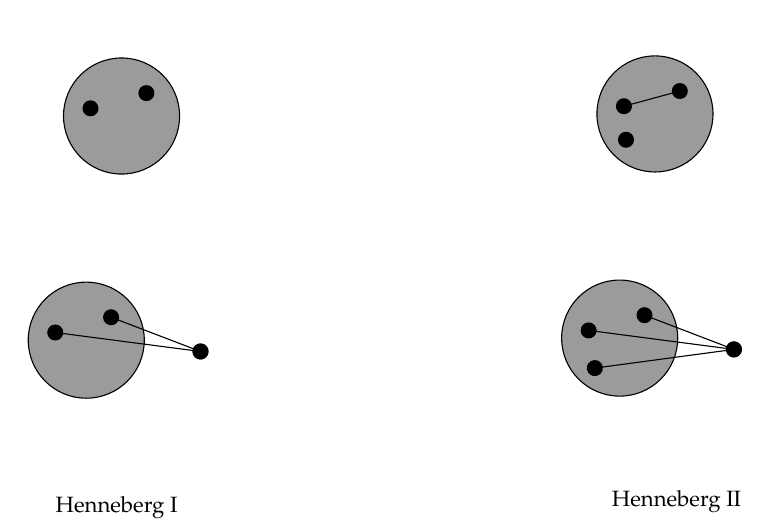
\begin{tikzpicture}[x=0.75pt,y=0.75pt,yscale=-1,xscale=1]
%uncomment if require: \path (0,294); %set diagram left start at 0, and has height of 294

%Shape: Circle [id:dp4412438273029411]
\draw  [fill={rgb, 255:red, 155; green, 155; blue, 155 }  ,fill opacity=1 ] (145.08,51.04) .. controls (145.08,35.6) and (157.6,23.08) .. (173.04,23.08) .. controls (188.48,23.08) and (201,35.6) .. (201,51.04) .. controls (201,66.48) and (188.48,79) .. (173.04,79) .. controls (157.6,79) and (145.08,66.48) .. (145.08,51.04) -- cycle ;
%Straight Lines [id:da6719764672917108]
\draw    (158.08,47.34) ;
\draw [shift={(158.08,47.34)}, rotate = 0] [color={rgb, 255:red, 0; green, 0; blue, 0 }  ][fill={rgb, 255:red, 0; green, 0; blue, 0 }  ][line width=0.75]      (0, 0) circle [x radius= 3.35, y radius= 3.35]   ;
%Straight Lines [id:da6181455657572694]
\draw    (185,40) ;
\draw [shift={(185,40)}, rotate = 0] [color={rgb, 255:red, 0; green, 0; blue, 0 }  ][fill={rgb, 255:red, 0; green, 0; blue, 0 }  ][line width=0.75]      (0, 0) circle [x radius= 3.35, y radius= 3.35]   ;
%Shape: Circle [id:dp41907435303254537]
\draw  [fill={rgb, 255:red, 155; green, 155; blue, 155 }  ,fill opacity=1 ] (128.08,159.04) .. controls (128.08,143.6) and (140.6,131.08) .. (156.04,131.08) .. controls (171.48,131.08) and (184,143.6) .. (184,159.04) .. controls (184,174.48) and (171.48,187) .. (156.04,187) .. controls (140.6,187) and (128.08,174.48) .. (128.08,159.04) -- cycle ;
%Straight Lines [id:da5231318408198586]
\draw    (141.08,155.34) ;
\draw [shift={(141.08,155.34)}, rotate = 0] [color={rgb, 255:red, 0; green, 0; blue, 0 }  ][fill={rgb, 255:red, 0; green, 0; blue, 0 }  ][line width=0.75]      (0, 0) circle [x radius= 3.35, y radius= 3.35]   ;
%Straight Lines [id:da9725080832536028]
\draw    (168,148) ;
\draw [shift={(168,148)}, rotate = 0] [color={rgb, 255:red, 0; green, 0; blue, 0 }  ][fill={rgb, 255:red, 0; green, 0; blue, 0 }  ][line width=0.75]      (0, 0) circle [x radius= 3.35, y radius= 3.35]   ;
%Straight Lines [id:da061078107428172324]
\draw    (211.08,164.49) -- (168,148) ;
\draw [shift={(211.08,164.49)}, rotate = 200.95] [color={rgb, 255:red, 0; green, 0; blue, 0 }  ][fill={rgb, 255:red, 0; green, 0; blue, 0 }  ][line width=0.75]      (0, 0) circle [x radius= 3.35, y radius= 3.35]   ;
%Straight Lines [id:da17622572078106158]
\draw    (211.08,164.49) -- (141.08,155.34) ;
\draw [shift={(211.08,164.49)}, rotate = 187.45] [color={rgb, 255:red, 0; green, 0; blue, 0 }  ][fill={rgb, 255:red, 0; green, 0; blue, 0 }  ][line width=0.75]      (0, 0) circle [x radius= 3.35, y radius= 3.35]   ;
%Shape: Circle [id:dp1077185002346912]
\draw  [fill={rgb, 255:red, 155; green, 155; blue, 155 }  ,fill opacity=1 ] (402.08,50.04) .. controls (402.08,34.6) and (414.6,22.08) .. (430.04,22.08) .. controls (445.48,22.08) and (458,34.6) .. (458,50.04) .. controls (458,65.48) and (445.48,78) .. (430.04,78) .. controls (414.6,78) and (402.08,65.48) .. (402.08,50.04) -- cycle ;
%Straight Lines [id:da28100620385230446]
\draw    (415.08,46.34) -- (442,39) ;
\draw [shift={(415.08,46.34)}, rotate = 344.74] [color={rgb, 255:red, 0; green, 0; blue, 0 }  ][fill={rgb, 255:red, 0; green, 0; blue, 0 }  ][line width=0.75]      (0, 0) circle [x radius= 3.35, y radius= 3.35]   ;
%Straight Lines [id:da7852320174709764]
\draw    (442,39) ;
\draw [shift={(442,39)}, rotate = 0] [color={rgb, 255:red, 0; green, 0; blue, 0 }  ][fill={rgb, 255:red, 0; green, 0; blue, 0 }  ][line width=0.75]      (0, 0) circle [x radius= 3.35, y radius= 3.35]   ;
%Shape: Circle [id:dp9682088462436504]
\draw  [fill={rgb, 255:red, 155; green, 155; blue, 155 }  ,fill opacity=1 ] (385.08,158.04) .. controls (385.08,142.6) and (397.6,130.08) .. (413.04,130.08) .. controls (428.48,130.08) and (441,142.6) .. (441,158.04) .. controls (441,173.48) and (428.48,186) .. (413.04,186) .. controls (397.6,186) and (385.08,173.48) .. (385.08,158.04) -- cycle ;
%Straight Lines [id:da3379441985669185]
\draw    (398.08,154.34) ;
\draw [shift={(398.08,154.34)}, rotate = 0] [color={rgb, 255:red, 0; green, 0; blue, 0 }  ][fill={rgb, 255:red, 0; green, 0; blue, 0 }  ][line width=0.75]      (0, 0) circle [x radius= 3.35, y radius= 3.35]   ;
%Straight Lines [id:da3518764950782256]
\draw    (425,147) ;
\draw [shift={(425,147)}, rotate = 0] [color={rgb, 255:red, 0; green, 0; blue, 0 }  ][fill={rgb, 255:red, 0; green, 0; blue, 0 }  ][line width=0.75]      (0, 0) circle [x radius= 3.35, y radius= 3.35]   ;
%Straight Lines [id:da4393606767678726]
\draw    (468.08,163.49) -- (425,147) ;
\draw [shift={(468.08,163.49)}, rotate = 200.95] [color={rgb, 255:red, 0; green, 0; blue, 0 }  ][fill={rgb, 255:red, 0; green, 0; blue, 0 }  ][line width=0.75]      (0, 0) circle [x radius= 3.35, y radius= 3.35]   ;
%Straight Lines [id:da9869108008194412]
\draw    (468.08,163.49) -- (398.08,154.34) ;
\draw [shift={(468.08,163.49)}, rotate = 187.45] [color={rgb, 255:red, 0; green, 0; blue, 0 }  ][fill={rgb, 255:red, 0; green, 0; blue, 0 }  ][line width=0.75]      (0, 0) circle [x radius= 3.35, y radius= 3.35]   ;
%Straight Lines [id:da2857165447033456]
\draw    (401.08,172.49) -- (468.08,163.49) ;
\draw [shift={(401.08,172.49)}, rotate = 352.35] [color={rgb, 255:red, 0; green, 0; blue, 0 }  ][fill={rgb, 255:red, 0; green, 0; blue, 0 }  ][line width=0.75]      (0, 0) circle [x radius= 3.35, y radius= 3.35]   ;
%Straight Lines [id:da5326196973625403]
\draw    (416.08,62.49) ;
\draw [shift={(416.08,62.49)}, rotate = 0] [color={rgb, 255:red, 0; green, 0; blue, 0 }  ][fill={rgb, 255:red, 0; green, 0; blue, 0 }  ][line width=0.75]      (0, 0) circle [x radius= 3.35, y radius= 3.35]   ;

% Text Node
\draw (140,233) node [anchor=north west][inner sep=0.75pt]  [font=\footnotesize] [align=left] {Henneberg I};
% Text Node
\draw (408,230) node [anchor=north west][inner sep=0.75pt]  [font=\footnotesize] [align=left] {Henneberg II};


\end{tikzpicture}
  \caption{}\label{HennebergI&II}
\end{figure}


In this section we consider the following variant of Henneberg I.
\begin{defn}[Henneberg I']
We define the following type operation:
\begin{itemize}
  \item Henneberg I': the new vertex is connected via two new edges to two old vertices which are end points of an old edge.
\end{itemize}
See Fig. \ref{HennebergI'}.
\end{defn}
\begin{figure}[htp]
  \centering


\tikzset{every picture/.style={line width=0.75pt}} %set default line width to 0.75pt

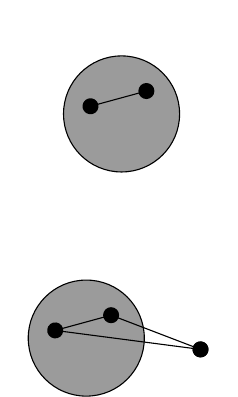
\begin{tikzpicture}[x=0.75pt,y=0.75pt,yscale=-1,xscale=1]
%uncomment if require: \path (0,237); %set diagram left start at 0, and has height of 237

%Shape: Circle [id:dp8497132848830529]
\draw  [fill={rgb, 255:red, 155; green, 155; blue, 155 }  ,fill opacity=1 ] (307.08,51.04) .. controls (307.08,35.6) and (319.6,23.08) .. (335.04,23.08) .. controls (350.48,23.08) and (363,35.6) .. (363,51.04) .. controls (363,66.48) and (350.48,79) .. (335.04,79) .. controls (319.6,79) and (307.08,66.48) .. (307.08,51.04) -- cycle ;
%Straight Lines [id:da1298783031017614]
\draw    (320.08,47.34) -- (347,40) ;
\draw [shift={(320.08,47.34)}, rotate = 344.74] [color={rgb, 255:red, 0; green, 0; blue, 0 }  ][fill={rgb, 255:red, 0; green, 0; blue, 0 }  ][line width=0.75]      (0, 0) circle [x radius= 3.35, y radius= 3.35]   ;
%Straight Lines [id:da31719465998079976]
\draw    (347,40) ;
\draw [shift={(347,40)}, rotate = 0] [color={rgb, 255:red, 0; green, 0; blue, 0 }  ][fill={rgb, 255:red, 0; green, 0; blue, 0 }  ][line width=0.75]      (0, 0) circle [x radius= 3.35, y radius= 3.35]   ;
%Shape: Circle [id:dp6065999172970378]
\draw  [fill={rgb, 255:red, 155; green, 155; blue, 155 }  ,fill opacity=1 ] (290.08,159.04) .. controls (290.08,143.6) and (302.6,131.08) .. (318.04,131.08) .. controls (333.48,131.08) and (346,143.6) .. (346,159.04) .. controls (346,174.48) and (333.48,187) .. (318.04,187) .. controls (302.6,187) and (290.08,174.48) .. (290.08,159.04) -- cycle ;
%Straight Lines [id:da560617837118635]
\draw    (303.08,155.34) -- (330,148) ;
\draw [shift={(303.08,155.34)}, rotate = 344.74] [color={rgb, 255:red, 0; green, 0; blue, 0 }  ][fill={rgb, 255:red, 0; green, 0; blue, 0 }  ][line width=0.75]      (0, 0) circle [x radius= 3.35, y radius= 3.35]   ;
%Straight Lines [id:da15372564810261813]
\draw    (330,148) ;
\draw [shift={(330,148)}, rotate = 0] [color={rgb, 255:red, 0; green, 0; blue, 0 }  ][fill={rgb, 255:red, 0; green, 0; blue, 0 }  ][line width=0.75]      (0, 0) circle [x radius= 3.35, y radius= 3.35]   ;
%Straight Lines [id:da5947345721631685]
\draw    (373.08,164.49) -- (330,148) ;
\draw [shift={(373.08,164.49)}, rotate = 200.95] [color={rgb, 255:red, 0; green, 0; blue, 0 }  ][fill={rgb, 255:red, 0; green, 0; blue, 0 }  ][line width=0.75]      (0, 0) circle [x radius= 3.35, y radius= 3.35]   ;
%Straight Lines [id:da37990258557512435]
\draw    (373.08,164.49) -- (303.08,155.34) ;
\draw [shift={(373.08,164.49)}, rotate = 187.45] [color={rgb, 255:red, 0; green, 0; blue, 0 }  ][fill={rgb, 255:red, 0; green, 0; blue, 0 }  ][line width=0.75]      (0, 0) circle [x radius= 3.35, y radius= 3.35]   ;




\end{tikzpicture}
  \caption{Henneberg I' operation}\label{HennebergI'}
\end{figure}
We will mainly focus on a special class of Laman graphs which we call Type I'.
\begin{defn}[Type I' Laman graphs]
  A Laman graph is called \textit{Type I'} if it can be constructed by a sequence of Henneberg I' operations.
\end{defn}
\iffalse
Given a type 1 Laman graph $\Gamma$, we choose a vertex $o\in V(\Gamma)$ as the base point and fix an edge $e\in E(\Gamma)$ such that $V(e)=\{o,v\}$. From the triple $(\Gamma,o,e)$, one can obtain a poset $\mathbf{H}_{\Gamma}(o,e)$ such that its underlying set is $V(\Gamma)$. For each $u\in \mathbf{H}_{\Gamma}(o,e)-\{o,v\}$, the lower cover set $C_u=\{u',u''\}$ has cardinality 2 and $u',u''$ are comparable. Furthermore, let $C_{<u}=\{v_1,v_2\}$ , we have $v_1\in C_{<v_2}$ or $v_2\in C_{<v_1}$.

From the poset $\mathbf{H}_{\Gamma}(o,e)$, we can choose a total order extension $\vec{\mathbf{H}}_{\Gamma}(o,e)$. Each total order extension corresponds to a sequence of Hennerberg moves which starts from $(o,e)$ and results in $\Gamma$.
\fi

Suppose $\Gamma$ is a Type I' Laman graph. We fix a vertex $o\in V(\Gamma)$ and an edge $e=[ov]\in E(\Gamma)$, the Laman graph $\Gamma$ can be constructed by a following sequence of Hennerberg operations
$$
\mathbf{H}_{\Gamma}(o,e)=[(e_0=e,v_1),(e_1,v_2),\dots,(e_{k-1},v_k)].
$$



Here $V(\Gamma)=\{o,v,v_1,\dots,v_k\}$. We start from an edge $e_0=e=[ov]$, then add a new vertex $v_1$ and draw two edges connecting $v_1$ and $o,v$. Repeat this procedure, we add a new vertex $v_i$ and choose an edge $e_{i-1}$ of the graph (we allow $e_{i-1}=e_{i'},i'<i-1$) and then connect $v_i$ and the vertices of $e_{i-1}$ by two edges. This can be illustrated by the picture as follows.
\begin{figure}[htb]
  \centering


\tikzset{every picture/.style={line width=0.75pt}} %set default line width to 0.75pt

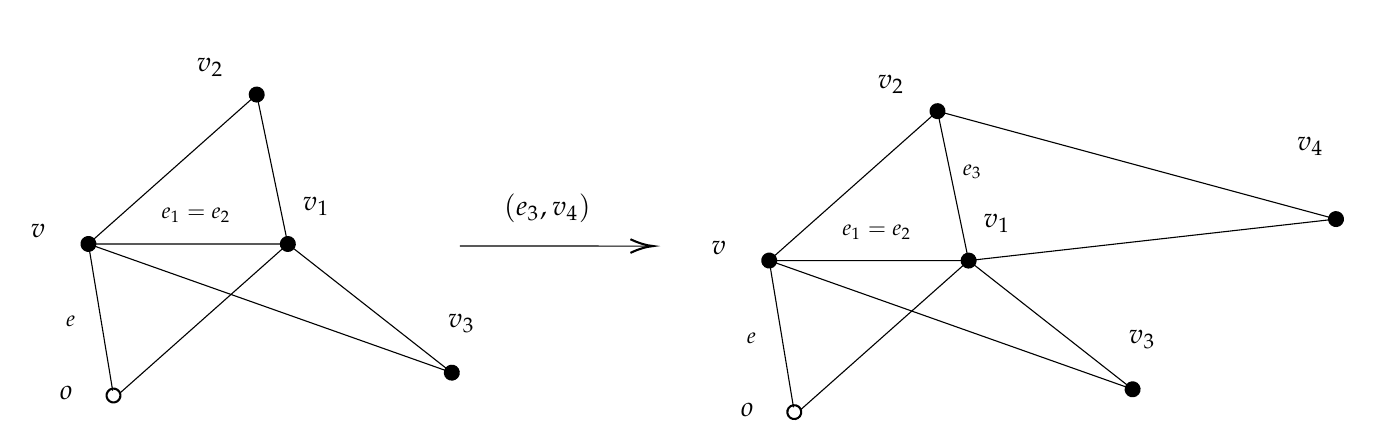
\begin{tikzpicture}[x=0.75pt,y=0.75pt,yscale=-1,xscale=1]
%uncomment if require: \path (0,284); %set diagram left start at 0, and has height of 284

%Straight Lines [id:da34453016663335045]
\draw    (38,116) -- (49.7,186.71) ;
\draw [shift={(50.08,189.02)}, rotate = 80.6] [color={rgb, 255:red, 0; green, 0; blue, 0 }  ][line width=0.75]      (0, 0) circle [x radius= 3.35, y radius= 3.35]   ;
\draw [shift={(38,116)}, rotate = 80.6] [color={rgb, 255:red, 0; green, 0; blue, 0 }  ][fill={rgb, 255:red, 0; green, 0; blue, 0 }  ][line width=0.75]      (0, 0) circle [x radius= 3.35, y radius= 3.35]   ;
%Straight Lines [id:da23846351567234625]
\draw    (38,116) -- (134.08,116.02) ;
%Straight Lines [id:da7317472081316405]
\draw    (53,188) -- (134.08,116.02) ;
\draw [shift={(134.08,116.02)}, rotate = 318.41] [color={rgb, 255:red, 0; green, 0; blue, 0 }  ][fill={rgb, 255:red, 0; green, 0; blue, 0 }  ][line width=0.75]      (0, 0) circle [x radius= 3.35, y radius= 3.35]   ;
%Straight Lines [id:da8790829958723019]
\draw    (134.08,116.02) -- (119.08,44.02) ;
%Straight Lines [id:da45626839654630835]
\draw    (38,116) -- (119.08,44.02) ;
\draw [shift={(119.08,44.02)}, rotate = 318.41] [color={rgb, 255:red, 0; green, 0; blue, 0 }  ][fill={rgb, 255:red, 0; green, 0; blue, 0 }  ][line width=0.75]      (0, 0) circle [x radius= 3.35, y radius= 3.35]   ;
%Straight Lines [id:da3217032538202462]
\draw    (38,116) -- (213.08,178.02) ;
%Straight Lines [id:da32856352918813814]
\draw    (134.08,116.02) -- (213.08,178.02) ;
\draw [shift={(213.08,178.02)}, rotate = 38.13] [color={rgb, 255:red, 0; green, 0; blue, 0 }  ][fill={rgb, 255:red, 0; green, 0; blue, 0 }  ][line width=0.75]      (0, 0) circle [x radius= 3.35, y radius= 3.35]   ;
%Straight Lines [id:da03364381956453277]
\draw    (366,124) -- (377.7,194.71) ;
\draw [shift={(378.08,197.02)}, rotate = 80.6] [color={rgb, 255:red, 0; green, 0; blue, 0 }  ][line width=0.75]      (0, 0) circle [x radius= 3.35, y radius= 3.35]   ;
\draw [shift={(366,124)}, rotate = 80.6] [color={rgb, 255:red, 0; green, 0; blue, 0 }  ][fill={rgb, 255:red, 0; green, 0; blue, 0 }  ][line width=0.75]      (0, 0) circle [x radius= 3.35, y radius= 3.35]   ;
%Straight Lines [id:da960646497046205]
\draw    (366,124) -- (462.08,124.02) ;
%Straight Lines [id:da46893865125491563]
\draw    (381,196) -- (462.08,124.02) ;
\draw [shift={(462.08,124.02)}, rotate = 318.41] [color={rgb, 255:red, 0; green, 0; blue, 0 }  ][fill={rgb, 255:red, 0; green, 0; blue, 0 }  ][line width=0.75]      (0, 0) circle [x radius= 3.35, y radius= 3.35]   ;
%Straight Lines [id:da6409845547594162]
\draw    (462.08,124.02) -- (447.08,52.02) ;
%Straight Lines [id:da07678649560674611]
\draw    (366,124) -- (447.08,52.02) ;
\draw [shift={(447.08,52.02)}, rotate = 318.41] [color={rgb, 255:red, 0; green, 0; blue, 0 }  ][fill={rgb, 255:red, 0; green, 0; blue, 0 }  ][line width=0.75]      (0, 0) circle [x radius= 3.35, y radius= 3.35]   ;
%Straight Lines [id:da46958944924801593]
\draw    (366,124) -- (541.08,186.02) ;
%Straight Lines [id:da2186402512738781]
\draw    (462.08,124.02) -- (541.08,186.02) ;
\draw [shift={(541.08,186.02)}, rotate = 38.13] [color={rgb, 255:red, 0; green, 0; blue, 0 }  ][fill={rgb, 255:red, 0; green, 0; blue, 0 }  ][line width=0.75]      (0, 0) circle [x radius= 3.35, y radius= 3.35]   ;
%Straight Lines [id:da03447631332638146]
\draw    (462.08,124.02) -- (639.08,104.02) ;
%Straight Lines [id:da31435411391819534]
\draw    (447.08,52.02) -- (639.08,104.02) ;
\draw [shift={(639.08,104.02)}, rotate = 15.15] [color={rgb, 255:red, 0; green, 0; blue, 0 }  ][fill={rgb, 255:red, 0; green, 0; blue, 0 }  ][line width=0.75]      (0, 0) circle [x radius= 3.35, y radius= 3.35]   ;
%Straight Lines [id:da7131917586733014]
\draw    (217,117) -- (308.08,117.02) ;
\draw [shift={(310.08,117.02)}, rotate = 180.01] [color={rgb, 255:red, 0; green, 0; blue, 0 }  ][line width=0.75]    (10.93,-3.29) .. controls (6.95,-1.4) and (3.31,-0.3) .. (0,0) .. controls (3.31,0.3) and (6.95,1.4) .. (10.93,3.29)   ;

% Text Node
\draw (23,183.4) node [anchor=north west][inner sep=0.75pt]    {$o$};
% Text Node
\draw (9,105.4) node [anchor=north west][inner sep=0.75pt]    {$v$};
% Text Node
\draw (140,92.4) node [anchor=north west][inner sep=0.75pt]    {$v_{1}$};
% Text Node
\draw (26,149.4) node [anchor=north west][inner sep=0.75pt]  [font=\footnotesize]  {$e$};
% Text Node
\draw (89,25.4) node [anchor=north west][inner sep=0.75pt]    {$v_{2}$};
% Text Node
\draw (72,97.4) node [anchor=north west][inner sep=0.75pt]  [font=\footnotesize]  {$e_{1} =e_{2}$};
% Text Node
\draw (210,148.4) node [anchor=north west][inner sep=0.75pt]    {$v_{3}$};
% Text Node
\draw (351,191.4) node [anchor=north west][inner sep=0.75pt]    {$o$};
% Text Node
\draw (337,113.4) node [anchor=north west][inner sep=0.75pt]    {$v$};
% Text Node
\draw (468,100.4) node [anchor=north west][inner sep=0.75pt]    {$v_{1}$};
% Text Node
\draw (354,157.4) node [anchor=north west][inner sep=0.75pt]  [font=\footnotesize]  {$e$};
% Text Node
\draw (417,33.4) node [anchor=north west][inner sep=0.75pt]    {$v_{2}$};
% Text Node
\draw (400,105.4) node [anchor=north west][inner sep=0.75pt]  [font=\footnotesize]  {$e_{1} =e_{2}$};
% Text Node
\draw (538,156.4) node [anchor=north west][inner sep=0.75pt]    {$v_{3}$};
% Text Node
\draw (458,76.4) node [anchor=north west][inner sep=0.75pt]  [font=\footnotesize]  {$e_{3}$};
% Text Node
\draw (619,63.4) node [anchor=north west][inner sep=0.75pt]    {$v_{4}$};
% Text Node
\draw (237,90.4) node [anchor=north west][inner sep=0.75pt]    {$( e_{3} ,v_{4})$};


\end{tikzpicture}
  \caption{}\label{}
\end{figure}


A Type I' Laman graph can be constructed from different sequences of Hennerberg moves $\mathbf{H}_{\Gamma}(o,e),
\mathbf{H}'_{\Gamma}(o,e)$ starting from $o, e$. 
Using the Arnold relation, we can show $W_{\Gamma}$ is exact in the
Jouanolou model and thus by the $L_{\infty}$-relation for chiral operations we reduce to the chiral operation for small
graphs. 
The Type I' condition ensure that the smaller graphs are still Type I' Laman. 
In this section, we will give the detailed construction of this outline thus providing an explicit recursive formula for the chiral operation on Type I' Laman graphs.

\begin{thm}\label{MainTheoremRecursiveRS}
Given a Type I' Laman graph $\Gamma$ and a sequence of Henneberg I' operations $\mathbf{H}_{\Gamma}(o,e)$ which constructs $\Gamma$, there are polynomial functions $$
\{f^{\Gamma,\mathbf{H}_{\Gamma}(o,e)}_{v,\vec{e}}\}_{v\in V(\Gamma)-\{o\}}\in \mathbb{C}[r_k,s_k]_{k=1,\dots,|V(\Gamma)|-2},\quad \mathbf{G}^{r,s}_{\Gamma,\mathbf{H}_{\Gamma}(o,e)}\in \mathbb{C}[r_k,s_k,\lambda^l_i]^{i\in V(\Gamma)-\{o\},l=1,2}_{k=1,\dots,|V(\Gamma)|-2},$$
  such that
$$
\mu_{V(\Gamma)}\left(W_{\Gamma}(\mathfrak{z}_{\vec{e}})\right)=\int_{([0,1]\times[0,1])^{|\mathbf{H}_{\Gamma}(o,e)|}}e^{\mathbf{W}^{r,s}_{\Gamma,\mathbf{H}_{\Gamma}(o,e)}}\cdot \mathbf{G}^{r,s}_{\Gamma,\mathbf{H}_{\Gamma}(o,e)}\cdot \bigwedge_{k=1,\dots,|\mathbf{H}_{\Gamma}(o,e)|} (dr_k\wedge ds_k)
$$
where
$$
    \mathbf{W}^{r,s}_{\Gamma,\mathbf{H}(o,e)}=\mathbf{W}^{r,s}_{\Gamma,\mathbf{H}(o,e)}(\lambda;\mathfrak{z}_{\vec{e}}):=\sum_{v\in V(\Gamma)-\{o\}}(\lambda_v|\sum_{e\in E(\Gamma)}f^{\Gamma,\mathbf{H}_{\Gamma}(o,e)}_{v,\vec{e}}\mathfrak{z}_{\vec{e}}).
$$
We can construct a new graph $\Gamma^{\star}$ using a Henneberg I' operations $\mathbf{H}_{\Gamma^{\star}}(o,e)=[\mathbf{H}_{\Gamma}(o,e),(e^\triangleright,\star)]$. Then we have the following recursive formulas for $\mu_{V(\Gamma^{\star})}\left(W_{\Gamma^{\star}}(\mathfrak{z}_{\vec{e}})\right)$:

  1) If $\star$ is connected to $i,j$ (i.e., $\vec{e^\triangleright}=ij$), then we introduce new variables
  $$
  \begin{cases}
    \mathfrak{z}^\triangleright_{ij}=\mathfrak{z}_{ij}+(1-r_{\star})(\mathfrak{z}_{\star j}-\mathfrak{z}_{\star i}-\mathfrak{z}_{ij}), & \\
   \mathfrak{z}^\triangleright_{\vec{e}}=\mathfrak{z}_{\vec{e}} , & \mbox{if}\ \vec{e}\neq ij,\\
   \lambda^\triangleright_i= \lambda_i+(1-s_{\star})\lambda_{\star},&\\
   \lambda^\triangleright_j= \lambda_j+s_{\star}\lambda_{\star},&\\
   \lambda^\triangleright_v=\lambda_v,& \mbox{if}\ v\neq i,j.
  \end{cases}
  $$
 \iffalse
  $$
\mu_{V(\Gamma^{\star})}\left(W_{\Gamma^{\star}}(\mathfrak{z}_{\vec{e}})\right)=\int_{([0,1]\times[0,1])^{|\mathbf{H}_{\Gamma}(o,e)|+1}}e^{\mathbf{W}^{r,s}_{\Gamma,\mathbf{H}_{\Gamma}(o,e)}}\cdot \mathbf{G}^{r,s}_{\Gamma^{\star},\mathbf{H}_{\Gamma^{\star}}(o,e)}\cdot (dr_{\star}\wedge ds_{\star})\bigwedge_{k=1,\dots,|\mathbf{H}_{\Gamma^{\star}}(o,e)|} (dr_k\wedge ds_k)
$$
\fi
  \iffalse
\begin{align*}
& \mu_{V(\Gamma)}\left(W^{r,s}_{\Gamma^{\star}}(\mathfrak{z}_{\vec{e}})\right)  = \int_{([0,1]\times[0,1])^{|\mathbf{H}_{\Gamma}(o,e)|+1}} e^{\mathbf{W}^{r,s}_{\Gamma,\mathbf{H}_{\Gamma}(o,e)}+(1-r_{\star})\left(\partial_{\mathfrak{z}_{ij}}\mathbf{W}^{r,s}_{\Gamma,\mathbf{H}_{\Gamma}(o,e)}|\mathfrak{z}_{\star j}-\mathfrak{z}_{\star i}-\mathfrak{z}_{ij}\right)-\left((1-s_{\star})\mathfrak{z}_{\star i}+s_{\star}\mathfrak{z}_{\star j}|\lambda_{\star}\right)} \\
   & \cdot e^{\left(((1-s_{\star})\partial_{\lambda_i}+s_{\star}\partial_{\lambda_j})(\mathbf{W}^{r,s}_{\Gamma,\mathbf{H}_{\Gamma}(o,e)}+(1-r_{\star})(\partial_{\mathfrak{z}_{ij}}\mathbf{W}^{r,s}_{\Gamma,\mathbf{H}_{\Gamma}(o,e)}|\mathfrak{z}_{\star j}-\mathfrak{z}_{\star i}-\mathfrak{z}_{ij}))|\lambda_{\star}\right)}\cdot \left(\partial_{\mathfrak{z}_{ij}}\mathbf{W}^{r,s}_{\Gamma,\mathbf{H}_{\Gamma}(o,e)}\wedge\lambda_{\star}\right)\cdot r_{\star}\\
   &\cdot  \mathbf{G}^{r,s}_{\Gamma,\mathbf{H}_{\Gamma}(o,e)}(\lambda_1,\dots,\lambda_i+(1-s_{\star})\lambda_{\star},\dots,\lambda_j+s_{\star}\lambda_{\star},\dots,\lambda_{n})\cdot (dr_{\star}\wedge ds_{\star})\cdot \bigwedge_{k=1,\dots,|\mathbf{H}_{\Gamma}(o,e)|} (dr_k\wedge ds_k)
\end{align*}
\fi
\begin{align*}
      \mathbf{W}^{r,s}_{\Gamma^{\star},\mathbf{H}_{\Gamma^{\star}}(o,e)} &= \mathbf{W}^{r,s}_{\Gamma,\mathbf{H}(o,e)}(\lambda^\triangleright;\mathfrak{z}^\triangleright_{\vec{e}}) -\left(\lambda_{\star}|(1-s_{\star})\mathfrak{z}_{\star i}+s_{\star}\mathfrak{z}_{\star j}\right) \\
   & =\sum_{v\in V(\Gamma)-o}(\lambda^\triangleright_v|\sum_{e\in E(\Gamma)}f^{\mathbf{H}_{\Gamma}}_{v,\vec{e}}\mathfrak{z}^\triangleright_{\vec{e}})-\left(\lambda_{\star}|(1-s_{\star})\mathfrak{z}_{\star i}+s_{\star}\mathfrak{z}_{\star j}\right).
\end{align*}
\begin{align*}
  \mathbf{G}^{r,s}_{\Gamma^{\star},\mathbf{H}_{\Gamma^{\star}}(o,e)} &= \left(\partial_{\mathfrak{z}_{ij}}\mathbf{W}^{r,s}_{\Gamma,\mathbf{H}_{\Gamma}(o,e)}(\lambda;\mathfrak{z}_{\vec{e}})\wedge\lambda_{\star}\right)\cdot  r_{\star}\cdot\mathbf{G}^{r,s}_{\Gamma,\mathbf{H}_{\Gamma}(o,e)}(\lambda^\triangleright) \\
   & =\left(\partial_{\mathfrak{z}_{ij}}\mathbf{W}^{r,s}_{\Gamma,\mathbf{H}_{\Gamma}(o,e)}(\lambda;\mathfrak{z}_{\vec{e}})\wedge\lambda_{\star}\right)\cdot r_{\star}\cdot\mathbf{G}^{r,s}_{\Gamma,\mathbf{H}_{\Gamma}(o,e)}(\lambda_1,\dots,\lambda_i+(1-s_{\star})\lambda_{\star},\dots,\lambda_j+s_{\star}\lambda_{\star},\dots,\lambda_{n})\cdot
\end{align*}
\iffalse
  2) If $\star$ is joint with $i,o$, then
\begin{align*}
& \mu_{V(\Gamma)}\left(W^{r,s}_{\Gamma^{\star}}(\mathfrak{z}_{\vec{e}})\right)  = \int_{([0,1]\times[0,1])^{|\mathbf{H}_{\Gamma}(o,e)|+1}} e^{\mathbf{W}^{r,s}_{\Gamma,\mathbf{H}_{\Gamma}(o,e)}+(1-r_{\star})\left(\partial_{\mathfrak{z}_{io}}\mathbf{W}^{r,s}_{\Gamma,\mathbf{H}_{\Gamma}(o,e)}|\mathfrak{z}_{\star o}-\mathfrak{z}_{\star i}-\mathfrak{z}_{io}\right)-\left((1-s_{\star})\mathfrak{z}_{\star i}+s_{\star}\mathfrak{z}_{\star o}|\lambda_{\star}\right)} \\
   & \cdot e^{\left((1-s_{\star})\partial_{\lambda_i}(\mathbf{W}^{r,s}_{\Gamma,\mathbf{H}_{\Gamma}(o,e)}+(1-r_{\star})(\partial_{\mathfrak{z}_{io}}\mathbf{W}^{r,s}_{\Gamma,\mathbf{H}_{\Gamma}(o,e)}|\mathfrak{z}_{\star o}-\mathfrak{z}_{\star i}-\mathfrak{z}_{io}))|\lambda_{\star}\right)}\cdot \left(\partial_{\mathfrak{z}_{io}}\mathbf{W}^{r,s}_{\Gamma,\mathbf{H}_{\Gamma}(o,e)}\wedge\lambda_{\star}\right)\cdot r_{\star}\\
   &\cdot  \mathbf{G}^{r,s}_{\Gamma,\mathbf{H}_{\Gamma}(o,e)}(\lambda_1,\dots,\lambda_i+(1-s_{\star})\lambda_{\star},\dots,\lambda_{n})\cdot (dr_{\star}\wedge ds_{\star})\cdot \bigwedge_{k=1,\dots,|\mathbf{H}_{\Gamma}(o,e)|} (dr_k\wedge ds_k)
\end{align*}
\fi
  1)If $\star$ is connected to $i,o$ (i.e., $\vec{e^\triangleright}=io$), then we introduce new variables
  $$
  \begin{cases}
    \mathfrak{z}^\triangleright_{io}=\mathfrak{z}_{io}+(1-r_{\star})(\mathfrak{z}_{\star o}-\mathfrak{z}_{\star i}-\mathfrak{z}_{io}), & \\
   \mathfrak{z}^\triangleright_{\vec{e}}=\mathfrak{z}_{\vec{e}} , & \mbox{if}\ \vec{e}\neq io,\\
   \lambda^\triangleright_i= \lambda_i+(1-s_{\star})\lambda_{\star},&\\
   \lambda^\triangleright_v=\lambda_v,& \mbox{if}\ v\neq i.
  \end{cases}
  $$
 \iffalse
  $$
\mu_{V(\Gamma^{\star})}\left(W_{\Gamma^{\star}}(\mathfrak{z}_{\vec{e}})\right)=\int_{([0,1]\times[0,1])^{|\mathbf{H}_{\Gamma}(o,e)|+1}}e^{\mathbf{W}^{r,s}_{\Gamma,\mathbf{H}_{\Gamma}(o,e)}}\cdot \mathbf{G}^{r,s}_{\Gamma^{\star},\mathbf{H}_{\Gamma^{\star}}(o,e)}\cdot (dr_{\star}\wedge ds_{\star})\bigwedge_{k=1,\dots,|\mathbf{H}_{\Gamma^{\star}}(o,e)|} (dr_k\wedge ds_k)
$$
\fi
  \iffalse
\begin{align*}
& \mu_{V(\Gamma)}\left(W^{r,s}_{\Gamma^{\star}}(\mathfrak{z}_{\vec{e}})\right)  = \int_{([0,1]\times[0,1])^{|\mathbf{H}_{\Gamma}(o,e)|+1}} e^{\mathbf{W}^{r,s}_{\Gamma,\mathbf{H}_{\Gamma}(o,e)}+(1-r_{\star})\left(\partial_{\mathfrak{z}_{ij}}\mathbf{W}^{r,s}_{\Gamma,\mathbf{H}_{\Gamma}(o,e)}|\mathfrak{z}_{\star j}-\mathfrak{z}_{\star i}-\mathfrak{z}_{ij}\right)-\left((1-s_{\star})\mathfrak{z}_{\star i}+s_{\star}\mathfrak{z}_{\star j}|\lambda_{\star}\right)} \\
   & \cdot e^{\left(((1-s_{\star})\partial_{\lambda_i}+s_{\star}\partial_{\lambda_j})(\mathbf{W}^{r,s}_{\Gamma,\mathbf{H}_{\Gamma}(o,e)}+(1-r_{\star})(\partial_{\mathfrak{z}_{ij}}\mathbf{W}^{r,s}_{\Gamma,\mathbf{H}_{\Gamma}(o,e)}|\mathfrak{z}_{\star j}-\mathfrak{z}_{\star i}-\mathfrak{z}_{ij}))|\lambda_{\star}\right)}\cdot \left(\partial_{\mathfrak{z}_{ij}}\mathbf{W}^{r,s}_{\Gamma,\mathbf{H}_{\Gamma}(o,e)}\wedge\lambda_{\star}\right)\cdot r_{\star}\\
   &\cdot  \mathbf{G}^{r,s}_{\Gamma,\mathbf{H}_{\Gamma}(o,e)}(\lambda_1,\dots,\lambda_i+(1-s_{\star})\lambda_{\star},\dots,\lambda_j+s_{\star}\lambda_{\star},\dots,\lambda_{n})\cdot (dr_{\star}\wedge ds_{\star})\cdot \bigwedge_{k=1,\dots,|\mathbf{H}_{\Gamma}(o,e)|} (dr_k\wedge ds_k)
\end{align*}
\fi
\begin{align*}
      \mathbf{W}^{r,s}_{\Gamma^{\star},\mathbf{H}_{\Gamma^{\star}}(o,e)} &= \mathbf{W}^{r,s}_{\Gamma,\mathbf{H}(o,e)}(\lambda^\triangleright;\mathfrak{z}^\triangleright_{\vec{e}}) -\left(\lambda_{\star}|(1-s_{\star})\mathfrak{z}_{\star i}+s_{\star}\mathfrak{z}_{\star o}\right)\\
   & =\sum_{v\in V(\Gamma)-o}(\lambda^\triangleright_v|\sum_{e\in E(\Gamma)}f^{\mathbf{H}_{\Gamma}}_{v,\vec{e}}\mathfrak{z}^\triangleright_{\vec{e}})-\left(\lambda_{\star}|(1-s_{\star})\mathfrak{z}_{\star i}+s_{\star}\mathfrak{z}_{\star o}\right).
\end{align*}
\begin{align*}
  \mathbf{G}^{r,s}_{\Gamma^{\star},\mathbf{H}_{\Gamma^{\star}}(o,e)} &= \left(\partial_{\mathfrak{z}_{io}}\mathbf{W}^{r,s}_{\Gamma,\mathbf{H}_{\Gamma}(o,e)}(\lambda;\mathfrak{z}_{\vec{e}})\wedge\lambda_{\star}\right)\cdot  r_{\star}\cdot\mathbf{G}^{r,s}_{\Gamma,\mathbf{H}_{\Gamma}(o,e)}(\lambda^\triangleright) \\
   & =\left(\partial_{\mathfrak{z}_{io}}\mathbf{W}^{r,s}_{\Gamma,\mathbf{H}_{\Gamma}(o,e)}(\lambda;\mathfrak{z}_{\vec{e}})\wedge\lambda_{\star}\right)\cdot r_{\star}\cdot\mathbf{G}^{r,s}_{\Gamma,\mathbf{H}_{\Gamma}(o,e)}(\lambda_1,\dots,\lambda_i+(1-s_{\star})\lambda_{\star},\dots,\lambda_{n})\cdot
\end{align*}

\end{thm}

\iffalse
We have following corollaries.
\begin{cor}
  The value $\mu_{V(\Gamma)}\left(W_{\Gamma}(\mathfrak{z}_{\vec{e}})\right)$ for a type 1 Lamman graph is determined by the chiral 2-operation.
\end{cor}
\fi

Using the above formula, we can write the formulas for some loop diagrams and match with results in \cite{Gaiotto:2024gii}. 
The remarkable thing is that, the chiral operation on Type I' Laman graph is completely constrained by the $L_{\infty}
$-relations and can be solved recursively without knowing Feynman integrals. 
In other words, the recursive formula gives another way to compute the complicated Feynman integrals. 
We provide some explicit examples.

\subsection{Example: one-loop diagrams}

\begin{figure}[htp]
  \centering


\tikzset{every picture/.style={line width=0.75pt}} %set default line width to 0.75pt

\begin{tikzpicture}[x=0.75pt,y=0.75pt,yscale=-1,xscale=1]
%uncomment if require: \path (0,251); %set diagram left start at 0, and has height of 251

%Straight Lines [id:da9500111546942909]
\draw    (121,84) -- (132.7,154.71) ;
\draw [shift={(133.08,157.02)}, rotate = 80.6] [color={rgb, 255:red, 0; green, 0; blue, 0 }  ][line width=0.75]      (0, 0) circle [x radius= 3.35, y radius= 3.35]   ;
\draw [shift={(121,84)}, rotate = 80.6] [color={rgb, 255:red, 0; green, 0; blue, 0 }  ][fill={rgb, 255:red, 0; green, 0; blue, 0 }  ][line width=0.75]      (0, 0) circle [x radius= 3.35, y radius= 3.35]   ;
%Straight Lines [id:da10944203577966927]
\draw    (437,91) -- (448.7,161.71) ;
\draw [shift={(449.08,164.02)}, rotate = 80.6] [color={rgb, 255:red, 0; green, 0; blue, 0 }  ][line width=0.75]      (0, 0) circle [x radius= 3.35, y radius= 3.35]   ;
\draw [shift={(437,91)}, rotate = 80.6] [color={rgb, 255:red, 0; green, 0; blue, 0 }  ][fill={rgb, 255:red, 0; green, 0; blue, 0 }  ][line width=0.75]      (0, 0) circle [x radius= 3.35, y radius= 3.35]   ;
%Straight Lines [id:da8673939939674462]
\draw    (437,91) -- (533.08,91.02) ;
%Straight Lines [id:da2921829490754293]
\draw    (452,163) -- (533.08,91.02) ;
\draw [shift={(533.08,91.02)}, rotate = 318.41] [color={rgb, 255:red, 0; green, 0; blue, 0 }  ][fill={rgb, 255:red, 0; green, 0; blue, 0 }  ][line width=0.75]      (0, 0) circle [x radius= 3.35, y radius= 3.35]   ;
%Straight Lines [id:da8223860172487036]
\draw    (257,107) -- (348.08,107.02) ;
\draw [shift={(350.08,107.02)}, rotate = 180.01] [color={rgb, 255:red, 0; green, 0; blue, 0 }  ][line width=0.75]    (10.93,-3.29) .. controls (6.95,-1.4) and (3.31,-0.3) .. (0,0) .. controls (3.31,0.3) and (6.95,1.4) .. (10.93,3.29)   ;

% Text Node
\draw (106,151.4) node [anchor=north west][inner sep=0.75pt]    {$o$};
% Text Node
\draw (109,117.4) node [anchor=north west][inner sep=0.75pt]  [font=\footnotesize]  {$e$};
% Text Node
\draw (422,158.4) node [anchor=north west][inner sep=0.75pt]    {$o$};
% Text Node
\draw (533,63.4) node [anchor=north west][inner sep=0.75pt]    {$2$};
% Text Node
\draw (425,124.4) node [anchor=north west][inner sep=0.75pt]  [font=\footnotesize]  {$e$};
% Text Node
\draw (277,80.4) node [anchor=north west][inner sep=0.75pt]    {$( e,2)$};
% Text Node
\draw (102,74.4) node [anchor=north west][inner sep=0.75pt]    {$1$};
% Text Node
\draw (412,73.4) node [anchor=north west][inner sep=0.75pt]    {$1$};


\end{tikzpicture}
  \caption{}\label{}
\end{figure}


%\Gui{Fill in the proof}
We start from
$$
\lineW(\lambda;\mathfrak{z}_{\vec{e}})  =-(\lambda_1|\mathfrak{z}_{1o}).
$$
By the recursive formula, we have
\begin{align*}
  \triangleW(\lambda;\mathfrak{z}_{\vec{e}})  &=-(\lambda^\triangleright_1|\mathfrak{z}^\triangleright_{1o})-  (1-s_{2})\left(\lambda_{2}|\mathfrak{z}_{21 }\right)-s_2\left(\lambda_{2}|\mathfrak{z}_{2 o}\right)\\
   & =-\left(\lambda_1+(1-s_2)\lambda_2|\mathfrak{z}_{1o}+(1-r_2)(\mathfrak{z}_{2 o}-\mathfrak{z}_{21}-\mathfrak{z}_{1o})\right)-  (1-s_{2})\left(\lambda_{2}|\mathfrak{z}_{21 }\right)-s_2\left(\lambda_{2}|\mathfrak{z}_{2 o}\right)\\
   & =-\left(\lambda_1|\mathfrak{z}_{1o}\right)-\left(\lambda_1|(1-r_2)(\mathfrak{z}_{2 o}-\mathfrak{z}_{21}-\mathfrak{z}_{1o})\right)-\left((1-s_2)\lambda_2|(1-r_2)(\mathfrak{z}_{2 o}-\mathfrak{z}_{21}-\mathfrak{z}_{1o})\right)\\
   &-\left((1-s_2)\lambda_2|\mathfrak{z}_{1o}\right)-  (1-s_{2})\left(\lambda_{2}|\mathfrak{z}_{21 }\right)-s_2\left(\lambda_{2}|\mathfrak{z}_{2 o}\right)\\
   &=-(\lambda_1|\mathfrak{z}_{1o})-(\lambda_2|\mathfrak{z}_{2o})-(1-r_{2})\left(\lambda_1|\mathfrak{z}_{2 o}-\mathfrak{z}_{21}-\mathfrak{z}_{1o}\right)+r_2(1-s_2)\left(\lambda_2|\mathfrak{z}_{2 o}-\mathfrak{z}_{21}-\mathfrak{z}_{1o}\right).
\end{align*}


\iffalse
 \begin{align*}
&\triangleW(\lambda)  =\lineW(\lambda)+(1-r_{2})\left(\partial_{\mathfrak{z}_{1o}}\lineW(\lambda)|\mathfrak{z}_{2 o}-\mathfrak{z}_{21}-\mathfrak{z}_{1o}\right)-(1-s_{2})\left(\mathfrak{z}_{21 }|\lambda_{2}\right)\\
&-s_2\left(\mathfrak{z}_{2 o}|\lambda_{2}\right)+\left(((1-s_2)\partial_{\lambda_1})(\lineW(\lambda)+(1-r_{2})(\partial_{\mathfrak{z}_{1o}}\lineW(\lambda)|\mathfrak{z}_{2 o}-\mathfrak{z}_{21 }-\mathfrak{z}_{1o}))|\lambda_{2}\right)\\
&=-(\mathfrak{z}_{1o}|\lambda_1)-(\mathfrak{z}_{2o}|\lambda_2)-(1-r_{2})\left(\lambda_1|\mathfrak{z}_{2 o}-\mathfrak{z}_{21}-\mathfrak{z}_{1o}\right)+r_2(1-s_2)\left(\lambda_2|\mathfrak{z}_{2 o}-\mathfrak{z}_{21}-\mathfrak{z}_{1o}\right)
\end{align*}
\fi
$$
\triangleG=r_2\cdot (\partial_{\mathfrak{z}_{1o}}\lineW)\wedge \lambda_2=r_2\cdot \lambda_1\wedge\lambda_2.
$$
  The 3-operation is given by the formula
\begin{align*}
&\mu_{\{o,1,2\}}\left(P_{1o}(\mathfrak{z}_{1o})P_{12}(\mathfrak{z}_{12})P_{2o}(\mathfrak{z}_{2o})d\mathbf{z}^{\blacklozenge}_{\{o,1,2\}}\right)
\\
&=\int_{[0,1]\times[0,1]}e^{\triangleW(\lambda;\mathfrak{z}_{\vec{e}})}\cdot \triangleG\cdot dr_2ds_2\cdot d\mathbf{z}^{\blacklozenge}_o\\
&=- e^{-(\lambda_2|\mathfrak{z}_{2o})-(\lambda_1|\mathfrak{z}_{1o})}\cdot \lambda_1\wedge\lambda_2\left(\frac{1}{(\lambda_1|\mathfrak{z})(\lambda_2|\mathfrak{z})}-\frac{e^{-(\lambda_1|\mathfrak{z})}}{(\lambda_1|\mathfrak{z})((\lambda_1+\lambda_2)|\mathfrak{z})}-\frac{e^{(\lambda_2|\mathfrak{z})}}{(\lambda_2|\mathfrak{z})((\lambda_1+\lambda_2)|\mathfrak{z})}\right)\cdot d\mathbf{z}^{\blacklozenge}_o\\
&=- e^{-(\lambda_2|\mathfrak{z}_{2o})-(\lambda_1|\mathfrak{z}_{1o})}\cdot \lambda_1\wedge\lambda_2\cdot \int_{l_1+l_2\leq 1}e^{-l_1(\lambda_1|\mathfrak{z})+l_2(\lambda_2|\mathfrak{z})}dl_1dl_2\cdot d\mathbf{z}^{\blacklozenge}_o,
\end{align*}
where $\mathfrak{z}=\mathfrak{z}_{2 o}-\mathfrak{z}_{21}-\mathfrak{z}_{1o}$.

\subsection{Example: two-loop diagrams}

\begin{figure}[htp]


\tikzset{every picture/.style={line width=0.75pt}} %set default line width to 0.75pt

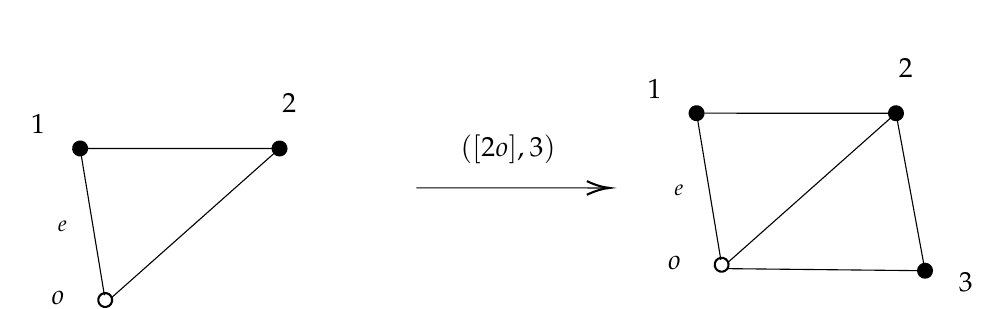
\begin{tikzpicture}[x=0.75pt,y=0.75pt,yscale=-1,xscale=1]
%uncomment if require: \path (0,251); %set diagram left start at 0, and has height of 251

%Straight Lines [id:da890181873775316]
\draw    (95,88) -- (106.7,158.71) ;
\draw [shift={(107.08,161.02)}, rotate = 80.6] [color={rgb, 255:red, 0; green, 0; blue, 0 }  ][line width=0.75]      (0, 0) circle [x radius= 3.35, y radius= 3.35]   ;
\draw [shift={(95,88)}, rotate = 80.6] [color={rgb, 255:red, 0; green, 0; blue, 0 }  ][fill={rgb, 255:red, 0; green, 0; blue, 0 }  ][line width=0.75]      (0, 0) circle [x radius= 3.35, y radius= 3.35]   ;
%Straight Lines [id:da9223610071211295]
\draw    (95,88) -- (191.08,88.02) ;
%Straight Lines [id:da11189533180737254]
\draw    (110,160) -- (191.08,88.02) ;
\draw [shift={(191.08,88.02)}, rotate = 318.41] [color={rgb, 255:red, 0; green, 0; blue, 0 }  ][fill={rgb, 255:red, 0; green, 0; blue, 0 }  ][line width=0.75]      (0, 0) circle [x radius= 3.35, y radius= 3.35]   ;
%Straight Lines [id:da9409890176578246]
\draw    (257,107) -- (348.08,107.02) ;
\draw [shift={(350.08,107.02)}, rotate = 180.01] [color={rgb, 255:red, 0; green, 0; blue, 0 }  ][line width=0.75]    (10.93,-3.29) .. controls (6.95,-1.4) and (3.31,-0.3) .. (0,0) .. controls (3.31,0.3) and (6.95,1.4) .. (10.93,3.29)   ;
%Straight Lines [id:da35422393324899293]
\draw    (392,71) -- (403.7,141.71) ;
\draw [shift={(404.08,144.02)}, rotate = 80.6] [color={rgb, 255:red, 0; green, 0; blue, 0 }  ][line width=0.75]      (0, 0) circle [x radius= 3.35, y radius= 3.35]   ;
\draw [shift={(392,71)}, rotate = 80.6] [color={rgb, 255:red, 0; green, 0; blue, 0 }  ][fill={rgb, 255:red, 0; green, 0; blue, 0 }  ][line width=0.75]      (0, 0) circle [x radius= 3.35, y radius= 3.35]   ;
%Straight Lines [id:da5782568358604838]
\draw    (392,71) -- (488.08,71.02) ;
%Straight Lines [id:da607564063352144]
\draw    (407,143) -- (488.08,71.02) ;
\draw [shift={(488.08,71.02)}, rotate = 318.41] [color={rgb, 255:red, 0; green, 0; blue, 0 }  ][fill={rgb, 255:red, 0; green, 0; blue, 0 }  ][line width=0.75]      (0, 0) circle [x radius= 3.35, y radius= 3.35]   ;
%Straight Lines [id:da8902609955225234]
\draw    (488.08,71.02) -- (502.08,146.9) ;
%Straight Lines [id:da2789811171892176]
\draw    (407.08,145.9) -- (502.08,146.9) ;
\draw [shift={(502.08,146.9)}, rotate = 0.6] [color={rgb, 255:red, 0; green, 0; blue, 0 }  ][fill={rgb, 255:red, 0; green, 0; blue, 0 }  ][line width=0.75]      (0, 0) circle [x radius= 3.35, y radius= 3.35]   ;

% Text Node
\draw (80,155.4) node [anchor=north west][inner sep=0.75pt]    {$o$};
% Text Node
\draw (191,60.4) node [anchor=north west][inner sep=0.75pt]    {$2$};
% Text Node
\draw (83,121.4) node [anchor=north west][inner sep=0.75pt]  [font=\footnotesize]  {$e$};
% Text Node
\draw (277,80.4) node [anchor=north west][inner sep=0.75pt]    {$([ 2o] ,3)$};
% Text Node
\draw (70,70.4) node [anchor=north west][inner sep=0.75pt]    {$1$};
% Text Node
\draw (377,138.4) node [anchor=north west][inner sep=0.75pt]    {$o$};
% Text Node
\draw (488,43.4) node [anchor=north west][inner sep=0.75pt]    {$2$};
% Text Node
\draw (380,104.4) node [anchor=north west][inner sep=0.75pt]  [font=\footnotesize]  {$e$};
% Text Node
\draw (367,53.4) node [anchor=north west][inner sep=0.75pt]    {$1$};
% Text Node
\draw (517,146.4) node [anchor=north west][inner sep=0.75pt]    {$3$};


\end{tikzpicture}
  \centering
  \caption{}\label{}
\end{figure}

 \begin{align*}
&   \agraphW  = \triangleW(\lambda^\triangleright;\mathfrak{z}^\triangleright_{\vec{e}}) -\left(\lambda_{3}|(1-s_{3})\mathfrak{z}_{3 2}+s_{3}\mathfrak{z}_{3 o}\right)\\
&=-(\lambda_1|\mathfrak{z}_{1o})-(\lambda_2|\mathfrak{z}_{2o})-\left(\lambda_{3}|\mathfrak{z}_{3o}\right)+\left(\lambda_1|-(1-r_{2})\mathfrak{z}_{[2 1o]}-(1-r_3)(1-r_2)\mathfrak{z}_{[32o]}\right)\\
&+\left(\lambda_2|(1-r_{3})(r_2(1-s_2)-1)\mathfrak{z}_{[3 2o]}+r_2(1-s_2)\mathfrak{z}_{[2 1o]}\right)\\
&+\left(\lambda_3|r_2(1-s_2)(1-s_3)\mathfrak{z}_{[21o]}+(1-s_3)(1-(1-r_3)(1-r_2(1-s_2)))\mathfrak{z}_{[32o]}\right)\\
\end{align*}
\begin{align*}
 \agraphG&=( \partial_{\mathfrak{z}_{2o}}\triangleW)\wedge\lambda_3\cdot r_3\cdot \triangleG(\lambda^\triangleright)\\
   &= -\left(\left((1-r_2)\lambda_1+(1-r_2(1-s_2))\lambda_2\right)\wedge \lambda_3\right)\cdot r_3r_2\cdot \left(\lambda_1\wedge\left(\lambda_2+(1-s_3)\lambda_3\right) \right)\\
     &
  \end{align*}
We have the following result
    \begin{align*}
&\mu_{\{o,1,2,3\}}\left(P_{3o}(\mathfrak{z}_{3o})P_{32}(\mathfrak{z}_{32})P_{1o}(\mathfrak{z}_{1o})P_{12}(\mathfrak{z}_{12})P_{2o}(\mathfrak{z}_{2o})d\mathbf{z}^{\blacklozenge}_{\{o,1,2,3\}}\right)
\\
&=\int_{([0,1]\times[0,1])^2}e^{\agraphW}\cdot \agraphG\cdot dr_2ds_2dr_3ds_3\cdot d\mathbf{z}^{\blacklozenge}_o.
  \end{align*}
    In particular, the constant term (when $\mathfrak{z}_{\vec{e}}=0$) is
    \begin{align*}
&\mu_{\{o,1,2,3\}}\left(P_{3o}P_{32}P_{1o}P_{12}P_{2o}d\mathbf{z}^{\blacklozenge}_{\{o,1,2,3\}}\right)
\\
&=\int_{([0,1]\times[0,1])^2}\agraphG\cdot dr_2ds_2dr_3ds_3\cdot d\mathbf{z}^{\blacklozenge}_o\\
&=\frac{1}{24}(\lambda_1\wedge(\lambda_3+2\lambda_2))\cdot (\lambda_3\wedge(\lambda_1+2\lambda_2))\cdot d\mathbf{z}^{\blacklozenge}_o.
  \end{align*}

  %  $$
    %\mu_{\{1<2<3<4\}}\left(P_{14}P_{12}P_{24}P_{32}P_{34}\right)=\frac{1}{24}(\lambda_1\wedge(\lambda_3+2\lambda_2))\cdot (\lambda_3\wedge(\lambda_1+2\lambda_2))
   % $$

\iffalse
  \begin{align*}
&   \agraphW  =\triangleW+(1-r_{3})\left(\partial_{\mathfrak{z}_{2o}}\triangleW|\mathfrak{z}_{3 o}-\mathfrak{z}_{32}-\mathfrak{z}_{2o}\right)-\left((1-s_{3})\mathfrak{z}_{3 2}|\lambda_{3}\right)\\
&-\left(s_3\mathfrak{z}_{3o}|\lambda_{3}\right)+\left(((1-s_{3})\partial_{\lambda_2})(\mathbf{W}_{\Gamma,\mathbf{H}_{\Gamma}(o,e)}(\lambda)+(1-r_{3})(\partial_{\mathfrak{z}_{2o}}\triangleW|\mathfrak{z}_{3 o}-\mathfrak{z}_{3 2}-\mathfrak{z}_{2o}))|\lambda_{3}\right)\\
&=-(\mathfrak{z}_{1o}|\lambda_1)-(\mathfrak{z}_{2o}|\lambda_2)-(1-r_{2})\left(\lambda_1|\mathfrak{z}_{2 o}-\mathfrak{z}_{21}-\mathfrak{z}_{1o}\right)+r_2(1-s_2)\left(\lambda_2|\mathfrak{z}_{2 o}-\mathfrak{z}_{21}-\mathfrak{z}_{1o}\right)\\
&+(1-r_{3})\left(-\lambda_2-(1-r_2)\lambda_1+r_2(1-s_2)\lambda_2|\mathfrak{z}_{3 o}-\mathfrak{z}_{32}-\mathfrak{z}_{2o}\right)-\left((1-s_{3})\mathfrak{z}_{3 2}|\lambda_{3}\right)-\left(s_3\mathfrak{z}_{3o}|\lambda_{3}\right)\\
&+(1-s_3)\left(-\mathfrak{z}_{2o}+r_2(1-s_2)(\mathfrak{z}_{2o}-\mathfrak{z}_{21}-\mathfrak{z}_{1o})|\lambda_3\right)-(1-s_3)(1-r_3)(1-r_2(1-s_2))\left(\mathfrak{z}_{3 o}-\mathfrak{z}_{32}-\mathfrak{z}_{2o}|\lambda_3\right)\\
%%&=-(\mathfrak{z}_{1o}|\lambda_1)-(\mathfrak{z}_{2o}|\lambda_2)-\left(\mathfrak{z}_{3o}|\lambda_{3}\right)-(1-r_{2})\left(\lambda_1|\mathfrak{z}_{2 o}-\mathfrak{z}_{21}-\mathfrak{z}_{1o}\right)+r_2(1-s_2)\left(\lambda_2|\mathfrak{z}_{2 o}-\mathfrak{z}_{21}-\mathfrak{z}_{1o}\right)\\
%%&+(1-r_{3})\left(-\lambda_2-(1-r_2)\lambda_1+r_2(1-s_2)\lambda_2|\mathfrak{z}_{3 o}-\mathfrak{z}_{32}-\mathfrak{z}_{2o}\right)+(1-s_{3})\left(\mathfrak{z}_{3 o}-\mathfrak{z}_{32}-\mathfrak{z}_{2o}|\lambda_{3}\right)\\
%%&+(1-s_3)\left(r_2(1-s_2)(\mathfrak{z}_{2o}-\mathfrak{z}_{21}-\mathfrak{z}_{1o})|\lambda_3\right)-(1-s_3)(1-r_3)(1-r_2(1-s_2))\left(\mathfrak{z}_{3 o}-\mathfrak{z}_{32}-\mathfrak{z}_{2o}|\lambda_3\right)\\
%%&=-(\mathfrak{z}_{1o}|\lambda_1)-(\mathfrak{z}_{2o}|\lambda_2)-\left(\mathfrak{z}_{3o}|\lambda_{3}\right)+\left(\lambda_1|-(1-r_{2})\mathfrak{z}_{[2 1o]}\right)+r_2(1-s_2)\left(\lambda_2|\mathfrak{z}_{[2 1o]}\right)\\
%%&+(1-r_{3})\left(-(1-r_2)\lambda_1+(r_2(1-s_2)-1)\lambda_2|\mathfrak{z}_{[3 2o]}\right)+(1-s_{3})\left(\lambda_{3}|\mathfrak{z}_{[32o]}\right)\\
%%&+r_2(1-s_2)(1-s_3)\left(\lambda_3|\mathfrak{z}_{[21o]}\right)-(1-s_3)(1-r_3)(1-r_2(1-s_2))\left(\lambda_3|\mathfrak{z}_{[32o]}\right)\\
&=-(\mathfrak{z}_{1o}|\lambda_1)-(\mathfrak{z}_{2o}|\lambda_2)-\left(\mathfrak{z}_{3o}|\lambda_{3}\right)+\left(\lambda_1|-(1-r_{2})\mathfrak{z}_{[2 1o]}-(1-r_3)(1-r_2)\mathfrak{z}_{[32o]}\right)\\
&+\left(\lambda_2|(1-r_{3})(r_2(1-s_2)-1)\mathfrak{z}_{[3 2o]}+r_2(1-s_2)\mathfrak{z}_{[2 1o]}\right)\\
&+\left(\lambda_3|r_2(1-s_2)(1-s_3)\mathfrak{z}_{[21o]}+(1-s_3)(1-(1-r_3)(1-r_2(1-s_2)))\mathfrak{z}_{[32o]}\right)\\
\end{align*}
\fi
\iffalse
  Let
  $$
t_1=r_2(1-s_2),t_3=(1-r_3)(1-t_1),\tilde{s}_1=\frac{(1-r_2)}{1-r_2(1-s_2)}=\frac{1-r_2}{1-t_1},\tilde{s}_3=1-s_3.
$$
$$
r_2=1-\tilde{s}_1(1-t_1),1-s_2=\frac{t_1}{1-\tilde{s}_1(1-t_1)}, 1-r_3=\frac{t_3}{1-t_1}.
$$
Then
\begin{align*}
      \agraphW &=-(\mathfrak{z}_{1o}|\lambda_1)-(\mathfrak{z}_{2o}|\lambda_2)-\left(\mathfrak{z}_{3o}|\lambda_{3}\right)+\left(\lambda_1|-\tilde{s}_1(1-t_1)\mathfrak{z}_{[2 1o]}+\tilde{s}_1t_3\mathfrak{z}_{[23o]}\right)\\
&+\left(\lambda_2|t_3\mathfrak{z}_{[23o]}+t_1\mathfrak{z}_{[2 1o]}\right)+\left(\lambda_3|t_1\tilde{s}_3\mathfrak{z}_{[21o]}-\tilde{s}_3(1-t_3)\mathfrak{z}_{[32o]}\right)\\
\end{align*}
\begin{align*}
  &( \partial_{\mathfrak{z}_{2o}}\triangleW)\wedge\lambda_3  \cdot r_2r_3dr_2ds_2dr_3ds_3\\
  &=\left((\tilde{s}_1\lambda_1+\lambda_2)\wedge\lambda_3 \right)\cdot (1-t_1)(1-\tilde{s}_1(1-t_1))(1-\frac{t_3}{1-t_1})d(1-\tilde{s}_1(1-t_1))d(\frac{t_1}{1-\tilde{s}_1(1-t_1)})d(\frac{t_3}{1-t_1})ds_3\\
   & =\left((\tilde{s}_1\lambda_1+\lambda_2)\wedge\lambda_3 \right)\cdot (1-t_1)(1-\frac{t_3}{1-t_1})d(1-\tilde{s}_1(1-t_1))dt_1d(\frac{t_3}{1-t_1})ds_3\\
   &=\left((\tilde{s}_1\lambda_1+\lambda_2)\wedge\lambda_3 \right)\cdot(1-t_1-t_3)d\tilde{s}_1dt_1dt_3ds_3.
\end{align*}
Finally
\begin{align*}
&\int_{\Delta_2\times\Delta_1\times\Delta_1}(1-t_3-t_1)\cdot(\lambda_3\wedge(s_1\lambda_1+\lambda_2))\cdot (\lambda_1\wedge(s_3\lambda_3+\lambda_2)) \cdot dt_1dt_3ds_1ds_3\\
&=\frac{1}{6}(\lambda_3\wedge(\frac{1}{2}\lambda_1+\lambda_2))\cdot (\lambda_1\wedge(\frac{1}{2}\lambda_3+\lambda_2))\\
&=\frac{1}{24}(\lambda_3\wedge(\lambda_1+2\lambda_2))\cdot (\lambda_1\wedge(\lambda_3+2\lambda_2)).
      \end{align*}
      \fi

\iffalse
\begin{proof}
$$
\begin{tabular}{|c|c|c|c|}
\hline
  & $\displaystyle \lambda _{1}$ & $\displaystyle \lambda _{2}$ & $\displaystyle \lambda _{3}$ \\
\hline
 $\displaystyle \mathfrak{z}_{1o}$ & $\displaystyle s_{1}( 1-t_{1}) -1=\boxed{l_{1o} -1}$ & $ $$\displaystyle -t_{1} =\boxed{l_{2o} -l_{3o} +l_{32} -1}$ & $\displaystyle -s_{3} t_{1}$$ $ \\
\hline
 $\displaystyle \mathfrak{z}_{2o}$ & $\displaystyle -s_{1}( 1-t_{1}) +s_{1} t_{2} =\boxed{\frac{l_{1o}( l_{2o} -1)}{2-l_{2o} +l_{34} -l_{32}}}$ & $\displaystyle -1+t_{1} +t_{2} =\boxed{l_{2o} -1}$ & $\displaystyle s_{3} t_{1} -s_{3}( 1-t_{2}) =\boxed{\frac{l_{3o}( l_{2o} -1)}{-l_{3o} +l_{32}}}$ \\
\hline
 $\displaystyle \mathfrak{z}_{12}$ & $\displaystyle s_{1}( 1-t_{1}) =\boxed{l_{1o}}$ & $\displaystyle t_{1} =\boxed{l_{2o} -l_{3o} +l_{32} -1}$ & $\displaystyle s_{3} t_{1} =\boxed{\frac{l_{3o}( l_{2o} -l_{3o} +l_{32} -1)}{-l_{3o} +l_{32}}}$ \\
\hline
 $\displaystyle \mathfrak{z}_{32}$ & $\displaystyle s_{1} t_{2} =\boxed{\frac{( l_{3o} -l_{32} +1) l_{1o}}{2-l_{2o} +l_{3o} -l_{32}}}$ & $\displaystyle t_{2} =\boxed{l_{3o} -l_{32} +1}$ & $\displaystyle s_{3}( 1-t_{2}) =\boxed{l_{3o}}$ \\
\hline
 $\displaystyle \mathfrak{z}_{3o}$ & $\displaystyle -s_{1} t_{2}$ & $\displaystyle -t_{2}$ & $\displaystyle -1+s_{3}( 1-t_{2}) =\boxed{l_{3o} -1}$$ $ \\
 \hline
\end{tabular}
$$

$$
 r=\frac{( l_{24} -1)}{l_{14} -l_{12}} =\frac{( l_{24} -1)}{2-l_{24} +l_{34} -l_{32}},\ \sum l_{e} =n-2
 $$

 $$
  s_{1} =\frac{l_{1o}}{2-l_{2o} +l_{3o} -l_{32}}=\frac{l_{1o}}{l_{1o} -l_{12}} ,\ \ \ \ s_{3} =\frac{l_{3o}}{-l_{3o} +l_{32}}
 $$
 We have
 \begin{align*}
    & F_{o,32}\wedge F_{o,3o}  \\
    & =(l_{3o}-l_{32}+1)^2\left(-\frac{l_{1o}}{l_{12}-l_{1o}}\lambda_1-\lambda_2+\frac{l_{3o}}{l_{3o}-l_{32}+1}\lambda_3\right)\wedge\left(\frac{l_{1o}}{l_{12}-l_{1o}}\lambda_1+\lambda_2+\frac{l_{3o}-1}{l_{3o}-l_{32}+1}\lambda_3\right)\\
    &=(l_{3o}-l_{32}+1)\left(\frac{l_{1o}}{l_{12}-l_{1o}}\lambda_1+\lambda_2\right)\wedge\lambda_3=(l_{3o}-l_{32}+1)\left(s_1\lambda_1+\lambda_2\right)\wedge\lambda_3
 \end{align*}

 \begin{align*}
    & F_{o,21}\wedge F_{o,2o}  \\
    & =(l_{12}-l_{1o}+1)(l_{2o}-1)\left(\frac{l_{1o}}{l_{12}-l_{1o}+1}\lambda_1+\lambda_2+\frac{l_{3o}}{l_{3o}-l_{32}}\lambda_3\right)\wedge \left(\frac{l_{1o}}{l_{12}-l_{1o}}\lambda_1+\lambda_2+\frac{l_{3o}}{l_{3o}-l_{32}}\lambda_3\right)\\
    &=\frac{(l_{2o}-1)l_{1o}}{l_{12}-l_{1o}}\left(\frac{l_{3o}}{l_{32}-l_{1o}}\lambda_3+\lambda_2\right)\wedge\lambda_1=\frac{(l_{2o}-1)l_{1o}}{l_{12}-l_{1o}}\left(s_3\lambda_3+\lambda_2\right)\wedge\lambda_1
 \end{align*}
 $$
 \mathbf{L}_{\Gamma,\mathbf{H}(o,e)}=\frac{l_{1o}-1}{l_{(23)}(l_{(23)}+1)l_{(3)}(l_{(3)}+1)}=\frac{1}{l_{1o}(l_{3o}-l_{32})(l_{3o}-l_{32}+1)}
 $$
 Then
 \begin{align*}
    &  \mu(W_{\Gamma})=\int_{\square_{\Gamma}}e^{\mathbf{W}_{\Gamma,\mathbf{H}(o,e)}(\lambda)}\cdot \mathbf{G}_{\Gamma,\mathbf{H}(o,e)}(\lambda)\bigwedge_{e\neq e_{o}}dl^{\Gamma}_{e} \\
    & =\int_{\square_{\Gamma}}e^{\mathbf{W}_{\Gamma,\mathbf{H}(o,e)}(\lambda)}\cdot (F_{o,32}\wedge F_{o,3o} )\cdot (F_{o,21}\wedge F_{o,2o} )\cdot\frac{1}{l_{1o}(l_{3o}-l_{32})(l_{3o}-l_{32}+1)}\cdot\bigwedge_{e\neq e_{o}}dl^{\Gamma}_{e}\\
    &=\int_{\square_{\Gamma}}e^{\mathbf{W}_{\Gamma,\mathbf{H}(o,e)}(\lambda)}\cdot (\lambda_3\wedge(s_1\lambda_1+\lambda_2))\cdot (\lambda_1\wedge(s_3\lambda_3+\lambda_2))\cdot \frac{(l_{2o}-1)}{(l_{12}-l_{1o})(l_{32}-l_{3o})}  \bigwedge_{e\neq e_{o}}dl^{\Gamma}_{e}\\
    &=\int_{\square_{\Gamma}}e^{\mathbf{W}_{\Gamma,\mathbf{H}(o,e)}(\lambda)}\cdot (\lambda_3\wedge(s_1\lambda_1+\lambda_2))\cdot (\lambda_1\wedge(s_3\lambda_3+\lambda_2))\\
    &\cdot (l_{2o}-1)d(l_{12}-l_{1o}+1)d(l_{32}-l_{3o}+1)d\frac{l_{1o}}{l_{1o} -l_{12}}d\frac{l_{3o}}{l_{3o} -l_{32}}\\
    &=\int_{\Delta_2\times\Delta_1\times\Delta_1}e^{   (\lambda_1|-s_1(1-t_1)\mathfrak{z}_{[124]}+s_1t_2\mathfrak{z}_{[324]})+ (\lambda_2|t_1\mathfrak{z}_{[124]}+t_2 \mathfrak{z}_{[324]})+      (\lambda_3|s_3t_1\mathfrak{z}_{[124]}-s_3(1-t_2)\mathfrak{z}_{[324]})}(1-t_2-t_1)\\
   &\cdot(\lambda_3\wedge(s_1\lambda_1+\lambda_2))\cdot (\lambda_1\wedge(s_3\lambda_3+\lambda_2)) \cdot dt_1dt_2ds_1ds_3\cdot e^{-(\lambda_1|\mathfrak{z}_{14})-(\lambda_2|\mathfrak{z}_{24})-(\lambda_3|\mathfrak{z}_{34})}
 \end{align*}

\end{proof}
\fi

\subsection{Example: 3-loop diagrams}
\begin{figure}[htp]
  \centering


\tikzset{every picture/.style={line width=0.75pt}} %set default line width to 0.75pt

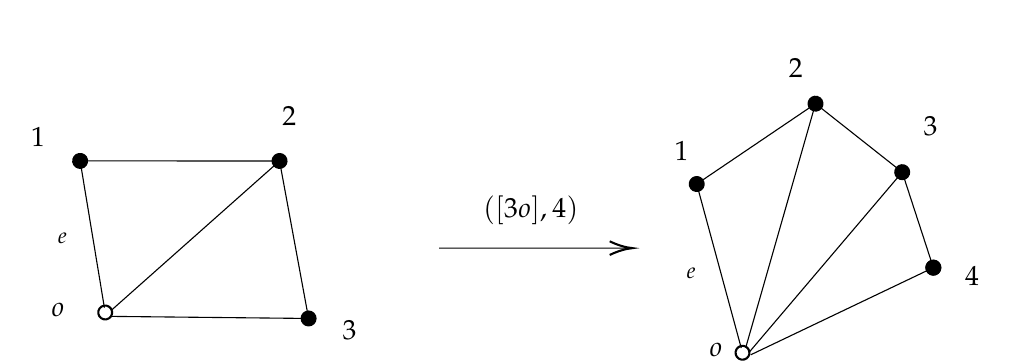
\begin{tikzpicture}[x=0.75pt,y=0.75pt,yscale=-1,xscale=1]
%uncomment if require: \path (0,251); %set diagram left start at 0, and has height of 251

%Straight Lines [id:da8477288815799091]
\draw    (257,107) -- (348.08,107.02) ;
\draw [shift={(350.08,107.02)}, rotate = 180.01] [color={rgb, 255:red, 0; green, 0; blue, 0 }  ][line width=0.75]    (10.93,-3.29) .. controls (6.95,-1.4) and (3.31,-0.3) .. (0,0) .. controls (3.31,0.3) and (6.95,1.4) .. (10.93,3.29)   ;
%Straight Lines [id:da19883481117548785]
\draw    (84,65) -- (95.7,135.71) ;
\draw [shift={(96.08,138.02)}, rotate = 80.6] [color={rgb, 255:red, 0; green, 0; blue, 0 }  ][line width=0.75]      (0, 0) circle [x radius= 3.35, y radius= 3.35]   ;
\draw [shift={(84,65)}, rotate = 80.6] [color={rgb, 255:red, 0; green, 0; blue, 0 }  ][fill={rgb, 255:red, 0; green, 0; blue, 0 }  ][line width=0.75]      (0, 0) circle [x radius= 3.35, y radius= 3.35]   ;
%Straight Lines [id:da6884477566281739]
\draw    (84,65) -- (180.08,65.02) ;
%Straight Lines [id:da8067150471550517]
\draw    (99,137) -- (180.08,65.02) ;
\draw [shift={(180.08,65.02)}, rotate = 318.41] [color={rgb, 255:red, 0; green, 0; blue, 0 }  ][fill={rgb, 255:red, 0; green, 0; blue, 0 }  ][line width=0.75]      (0, 0) circle [x radius= 3.35, y radius= 3.35]   ;
%Straight Lines [id:da7279525719966016]
\draw    (180.08,65.02) -- (194.08,140.9) ;
%Straight Lines [id:da874142011205592]
\draw    (99.08,139.9) -- (194.08,140.9) ;
\draw [shift={(194.08,140.9)}, rotate = 0.6] [color={rgb, 255:red, 0; green, 0; blue, 0 }  ][fill={rgb, 255:red, 0; green, 0; blue, 0 }  ][line width=0.75]      (0, 0) circle [x radius= 3.35, y radius= 3.35]   ;
%Straight Lines [id:da6454806350471596]
\draw    (381.08,76.13) -- (402.53,155.15) ;
\draw [shift={(403.14,157.42)}, rotate = 74.82] [color={rgb, 255:red, 0; green, 0; blue, 0 }  ][line width=0.75]      (0, 0) circle [x radius= 3.35, y radius= 3.35]   ;
\draw [shift={(381.08,76.13)}, rotate = 74.82] [color={rgb, 255:red, 0; green, 0; blue, 0 }  ][fill={rgb, 255:red, 0; green, 0; blue, 0 }  ][line width=0.75]      (0, 0) circle [x radius= 3.35, y radius= 3.35]   ;
%Straight Lines [id:da6618500472761442]
\draw    (381.08,76.13) -- (438.31,37.42) ;
%Straight Lines [id:da9255829903454396]
\draw    (404.67,155.03) -- (438.31,37.42) ;
\draw [shift={(438.31,37.42)}, rotate = 285.96] [color={rgb, 255:red, 0; green, 0; blue, 0 }  ][fill={rgb, 255:red, 0; green, 0; blue, 0 }  ][line width=0.75]      (0, 0) circle [x radius= 3.35, y radius= 3.35]   ;
%Straight Lines [id:da026400001424949693]
\draw    (438.31,37.42) -- (480.08,70.42) ;
%Straight Lines [id:da3023640696608898]
\draw    (406.14,157.42) -- (480.08,70.42) ;
\draw [shift={(480.08,70.42)}, rotate = 310.36] [color={rgb, 255:red, 0; green, 0; blue, 0 }  ][fill={rgb, 255:red, 0; green, 0; blue, 0 }  ][line width=0.75]      (0, 0) circle [x radius= 3.35, y radius= 3.35]   ;
%Straight Lines [id:da32497524909403896]
\draw    (407.08,158.42) -- (495.08,116.42) ;
\draw [shift={(495.08,116.42)}, rotate = 334.49] [color={rgb, 255:red, 0; green, 0; blue, 0 }  ][fill={rgb, 255:red, 0; green, 0; blue, 0 }  ][line width=0.75]      (0, 0) circle [x radius= 3.35, y radius= 3.35]   ;
%Straight Lines [id:da6118969901897813]
\draw    (480.08,70.42) -- (495.08,116.42) ;
\draw [shift={(495.08,116.42)}, rotate = 71.94] [color={rgb, 255:red, 0; green, 0; blue, 0 }  ][fill={rgb, 255:red, 0; green, 0; blue, 0 }  ][line width=0.75]      (0, 0) circle [x radius= 3.35, y radius= 3.35]   ;

% Text Node
\draw (277,80.4) node [anchor=north west][inner sep=0.75pt]    {$([ 3o] ,4)$};
% Text Node
\draw (69,132.4) node [anchor=north west][inner sep=0.75pt]    {$o$};
% Text Node
\draw (180,37.4) node [anchor=north west][inner sep=0.75pt]    {$2$};
% Text Node
\draw (72,98.4) node [anchor=north west][inner sep=0.75pt]  [font=\footnotesize]  {$e$};
% Text Node
\draw (59,47.4) node [anchor=north west][inner sep=0.75pt]    {$1$};
% Text Node
\draw (209,140.4) node [anchor=north west][inner sep=0.75pt]    {$3$};
% Text Node
\draw (369,54.4) node [anchor=north west][inner sep=0.75pt]    {$1$};
% Text Node
\draw (424,14.4) node [anchor=north west][inner sep=0.75pt]    {$2$};
% Text Node
\draw (489,42.4) node [anchor=north west][inner sep=0.75pt]    {$3$};
% Text Node
\draw (509,114.4) node [anchor=north west][inner sep=0.75pt]    {$4$};
% Text Node
\draw (386,151.4) node [anchor=north west][inner sep=0.75pt]    {$o$};
% Text Node
\draw (375,115.4) node [anchor=north west][inner sep=0.75pt]  [font=\footnotesize]  {$e$};


\end{tikzpicture}
  \caption{}\label{}
\end{figure}
\iffalse
The 5-point function is given by
\begin{align*}
   \bgraphW=& \int^1_0dr_2\int^1_0ds_4\int^1_0ds_2\int^1_0ds_1\int_{t_1+t_4\leq 1}dt_1dt_4\left(\lambda_1\wedge (s_4\lambda_4+s_4s_2\lambda_2+\lambda_3) \right)\left( (\lambda_4+s_2\lambda_2)\wedge (s_1\lambda_1+\lambda_3)\right)  \\
   & \cdot \left(\lambda_2\wedge (-s_1t_4\lambda_1-t_4\lambda_3+(s_4(1-t_4)-1)\lambda_4)\right)\cdot(1-t_4-t_1) r_2\cdot e^{\mathbf{W}_{\Gamma,\mathbf{H}(o,e)}(\lambda)}
\end{align*}
\fi

\iffalse
  \begin{align*}
        \bgraphW&=-(\mathfrak{z}_{1o}|\lambda_1)-(\mathfrak{z}_{2o}|\lambda_2)-\left(\mathfrak{z}_{3o}+(1-r_4)\mathfrak{z}_{[43o]}|\lambda_{3}+(1-s_4)\lambda_4\right)\\
        &+\left(\lambda_1|-(1-r_{2})\mathfrak{z}_{[2 1o]}-(1-r_3)(1-r_2)\mathfrak{z}_{[32o]}-(1-r_4)(1-r_3)(1-r_2)\mathfrak{z}_{[43o]}\right)\\
&+\left(\lambda_2|(1-r_4)(1-r_{3})(r_2(1-s_2)-1)\mathfrak{z}_{[43o]}+(1-r_{3})(r_2(1-s_2)-1)\mathfrak{z}_{[3 2o]}+r_2(1-s_2)\mathfrak{z}_{[2 1o]}\right)\\
&+\left(\lambda_3|r_2(1-s_2)(1-s_3)\mathfrak{z}_{[21o]}+(1-s_3)(1-(1-r_3)(1-r_2(1-s_2)))\mathfrak{z}_{[32o]}\right)\\
&+\left(\lambda_3|(1-r_4)(1-s_3)(1-(1-r_3)(1-r_2(1-s_2)))\mathfrak{z}_{[43o]}\right)\\
&+(1-s_4)\left(\lambda_4|r_2(1-s_2)(1-s_3)\mathfrak{z}_{[21o]}+(1-s_3)(1-(1-r_3)(1-r_2(1-s_2)))\mathfrak{z}_{[32o]}\right)\\
&+(1-s_4)\left(\lambda_4|(1-r_4)(1-s_3)(1-(1-r_3)(1-r_2(1-s_2)))\mathfrak{z}_{[43o]}\right)\\
&-\left((1-s_4)\mathfrak{z}_{43}+s_4\mathfrak{z}_{4o}|\lambda_4\right)
  \end{align*}

  We change the order of vertex to match the computation of [Gaiotto]
  $$
  \lambda_1\rightarrow\lambda_1,\lambda_2\rightarrow \lambda_3, \lambda_3\rightarrow \lambda_4
  $$
  and the new adding vertex is $\lambda_2$. Then we have
  \begin{align*}
      \agraphW &=-(\mathfrak{z}_{1o}|\lambda_1)-(\mathfrak{z}_{3o}|\lambda_3)-\left(\mathfrak{z}_{4o}|\lambda_{4}\right)+\left(\lambda_1|-\tilde{s}_1(1-t_1)\mathfrak{z}_{[3 1o]}+\tilde{s}_1t_4\mathfrak{z}_{[34o]}\right)\\
&+\left(\lambda_3|t_4\mathfrak{z}_{[34o]}+t_1\mathfrak{z}_{[3 1o]}\right)+\left(\lambda_4|t_1\tilde{s}_4\mathfrak{z}_{[31o]}-\tilde{s}_4(1-t_4)\mathfrak{z}_{[34o]}\right)\\
\end{align*}
$$
\partial_{\mathfrak{z}_{4o}}\agraphW=-\tilde{s}_1t_4\lambda_1-t_4\lambda_3+(\tilde{s}_4(1-t_4)-1)\lambda
_4
$$
  \begin{align*}
     &  \\
     \agraphG& =(1-t_4-t_1)\cdot(\lambda_4\wedge(\tilde{s}_1\lambda_1+\lambda_2))\cdot (\lambda_1\wedge(\tilde{s}_4\lambda_4+\lambda_3)) \cdot dt_1dt_4d\tilde{s}_1d\tilde{s}_4
  \end{align*}

  Then
  \begin{align*}
 &\bgraphG =  (1-t_4-t_1)r_2\cdot((\lambda_4+\tilde{s}_2\lambda_2)\wedge(\tilde{s}_1\lambda_1+\lambda_2))\cdot (\lambda_1\wedge(\tilde{s}_4(\lambda_4+\tilde{s}_2\lambda_2)+\lambda_3)) \\ &\cdot  (\lambda_2\wedge \partial_{\mathfrak{z}_{4o}}\agraphW)\cdot dt_1dt_4d\tilde{s}_1d\tilde{s}_4d\tilde{s}_2dr_2 \\
     &
  \end{align*}
\fi

By the same but tedious computation, one can obtain the formula for $\bgraphW$. Here we only compute $\bgraphG$.
We have
\begin{align*}
   \bgraphG&= r_4\cdot \agraphG(\lambda^\triangleright) \cdot(\partial_{\mathfrak{z}_{3o}}\agraphW)\wedge \lambda_4  \\
   &=r_4r_3r_2\cdot \left(\left((1-r_2)\lambda_1+(1-r_2(1-s_2))\lambda_2\right)\wedge (\lambda_3+(1-s_4)\lambda_4)\right) \\
   & \cdot\left(\lambda_1\wedge\left(\lambda_2+(1-s_3)\lambda_3+(1-s_3)(1-s_4)\lambda_4\right) \right)\\ &\cdot  \left(-(1-r_3)(1-r_2)\lambda_1+(1-r_3)(r_2(1-s_2)-1)\lambda_2+(-s_3-(1-s_3)(1-r_3)(1-r_2(1-s_2)))\lambda_3\right)\wedge \lambda_4
\end{align*}
The constant term (when $\mathfrak{z}_{\vec{e}}=0$) is
    \begin{align*}
&\mu_{\{o,1,2,3,4\}}\left(P_{4o}P_{43}P_{3o}P_{32}P_{1o}P_{12}P_{2o}d\mathbf{z}^{\blacklozenge}_{\{o,1,2,3,4\}}\right)
\\
&=\int_{([0,1]\times[0,1])^3}\bgraphG\cdot dr_2ds_2dr_3ds_3dr_4ds_4\cdot d\mathbf{z}^{\blacklozenge}_o\\
&=F(\lambda_1,\lambda_2,\lambda_3,\lambda_4)\cdot d\mathbf{z}^{\blacklozenge}_o.
  \end{align*}
  The polynomial $F(\lambda_1,\lambda_2,\lambda_3,\lambda_4)$ can be computed using computer and matches the
  computation in \cite{Gaiotto:2024gii}. See the maple code attached in the Appendix.

  \subsection{Proof of theorem \ref{MainTheoremRecursiveRS}} 
  Now we turn to the proof of Theorem \ref{MainTheoremRecursiveRS}. We need some lemmas.
\begin{lem}\label{IntegralXP}
We have the following integral formula for the product of derivatives of $x^i_{12}(\mathfrak{z})$ and $P_{12}(\mathfrak{w})$
  $$
G(\partial_{z^1_{1}},\partial_{z^2_{1}})x^i_{12}(\mathfrak{z})\cdot\left( F(\partial_{z^1_{1}},\partial_{z^2_{1}})\cdot P_{12}(\mathfrak{w})\right)=G(\partial_{\mathfrak{z}^1},\partial_{\mathfrak{z}^2})F(\partial_{\mathfrak{w}^1},\partial_{\mathfrak{w}^2})(-\partial_{\mathfrak{w}^i})\int^1_0P_{12}\left((1-s)\mathfrak{z}+s\mathfrak{w}\right)ds
  $$
  $$
  =\int^1_0G\left((1-s)\partial_{z^1_1},(1-s)\partial_{z^2_1}\right)F\left(s\partial_{z^1_1},s\partial_{z^2_1}\right)(-s\partial_{z^i_1})P_{12}\left((1-s)\mathfrak{z}+s\mathfrak{w}\right)ds,
  $$
  \iffalse
$$
G(\partial_{z^1_{1}},\partial_{z^2_{1}})P_{12}(\mathfrak{z})\cdot\left( F(\partial_{z^1_{1}},\partial_{z^2_{1}})\cdot x^i_{12}(\mathfrak{w})\right)=G(\partial_{\mathfrak{z}^1},\partial_{\mathfrak{z}^2})F(\partial_{\mathfrak{w}^1},\partial_{\mathfrak{w}^2})(-\partial_{\mathfrak{z}^i})\int^1_0P_{12}\left((1-s)\mathfrak{z}+s\mathfrak{w}\right)ds
  $$
  $$
  =\int^1_0G\left((1-s)\partial_{z^1_1},(1-s)\partial_{z^2_1}\right)F\left(s\partial_{z^1_1},s\partial_{z^2_1}\right)(-(1-s)\partial_{z^i_1})P_{12}\left((1-s)\mathfrak{z}+s\mathfrak{w}\right)ds.
  $$
  \fi
\end{lem}

\begin{proof}
The lemma follows from the following direct computation
  \begin{align*}
&      G(\partial_{z^1_{1}},\partial_{z^2_{1}})x^i_{12}(\mathfrak{z})\cdot\left( F(\partial_{z^1_{1}},\partial_{z^2_{1}})\cdot P_{12}(\mathfrak{w})\right)  \\ &=G(\partial_{\mathfrak{z}^1},\partial_{\mathfrak{z}^2})F(\partial_{\mathfrak{w}^1},\partial_{\mathfrak{w}^2})\left(x^i_{12}(\mathfrak{z})P_{12}(\mathfrak{w})\right)\\
     & =G(\partial_{\mathfrak{z}^1},\partial_{\mathfrak{z}^2})F(\partial_{\mathfrak{w}^1},\partial_{\mathfrak{w}^2})\left(\frac{x^i_{12}(\mathfrak{z})P_{12}(\mathfrak{z})}{\left(1+(x_{12}(\mathfrak{z})|\mathfrak{w}-\mathfrak{z})\right)^2}\right)\\
    &=  G(\partial_{\mathfrak{z}^1},\partial_{\mathfrak{z}^2})F(\partial_{\mathfrak{w}^1},\partial_{\mathfrak{w}^2})  \sum_{m=0}^{\infty}(-x_{12}(\mathfrak{z})|\mathfrak{w}-\mathfrak{z})^m(m+1)x^i_{12}(\mathfrak{z})P_{12}(\mathfrak{z}) \\
    &=G(\partial_{\mathfrak{z}^1},\partial_{\mathfrak{z}^2})F(\partial_{\mathfrak{w}^1},\partial_{\mathfrak{w}^2}) \sum_{m=0}^{\infty}(\partial_{z_1}|\mathfrak{w}-\mathfrak{z})^m\frac{-\partial_{z^1_1}P_{12}(\mathfrak{z})}{m!\cdot (m+2)}\\
    &=G(\partial_{\mathfrak{z}^1},\partial_{\mathfrak{z}^2})F(\partial_{\mathfrak{w}^1},\partial_{\mathfrak{w}^2}) \int^1_0e^{s(\partial_{z_1}|\mathfrak{w}-\mathfrak{z})}s\cdot (-\partial_{z^{i}_1})P_{12}(\mathfrak{z})ds\\
    &=G(\partial_{\mathfrak{z}^1},\partial_{\mathfrak{z}^2})F(\partial_{\mathfrak{w}^1},\partial_{\mathfrak{w}^2})(-\partial_{\mathfrak{w}^i})\int^1_0P_{12}\left((1-s)\mathfrak{z}+s\mathfrak{w}\right)ds\\
    &=\int^1_0G\left((1-s)\partial_{z^1_1},(1-s)\partial_{z^2_1}\right)F\left(s\partial_{z^1_1},s\partial_{z^2_1}\right)(-s\partial_{z^i_1})P_{12}\left((1-s)\mathfrak{z}+s\mathfrak{w}\right)ds.
  \end{align*}
\iffalse
  \begin{align*}
     & G(\partial_{z^1_{1}},\partial_{z^2_{1}})P_{12}(\mathfrak{z})\cdot\left( F(\partial_{z^1_{1}},\partial_{z^2_{1}})\cdot x^i_{12}(\mathfrak{w})\right)  \\ &=G(\partial_{\mathfrak{z}^1},\partial_{\mathfrak{z}^2})F(\partial_{\mathfrak{w}^1},\partial_{\mathfrak{w}^2})\left(x^i_{12}(\mathfrak{w})P_{12}(\mathfrak{z})\right)\\
     & =G(\partial_{\mathfrak{z}^1},\partial_{\mathfrak{z}^2})F(\partial_{\mathfrak{w}^1},\partial_{\mathfrak{w}^2})\left(\frac{x^i_{12}(\mathfrak{z})P_{12}(\mathfrak{z})}{1+(x_{12}(\mathfrak{z})|\mathfrak{w}-\mathfrak{z})}\right)\\
    &=  G(\partial_{\mathfrak{z}^1},\partial_{\mathfrak{z}^2})F(\partial_{\mathfrak{w}^1},\partial_{\mathfrak{w}^2})  \sum_{m=0}^{\infty}(-x_{12}(\mathfrak{z})|\mathfrak{w}-\mathfrak{z})^mx^i_{12}(\mathfrak{z})P_{12}(\mathfrak{z}) \\
    &=G(\partial_{\mathfrak{z}^1},\partial_{\mathfrak{z}^2})F(\partial_{\mathfrak{w}^1},\partial_{\mathfrak{w}^2}) \sum_{m=0}^{\infty}(\partial_{z_1}|\mathfrak{w}-\mathfrak{z})^m\frac{-\partial_{z^1_1}P_{12}(\mathfrak{z})}{(m+2)!}\\
    &=G(\partial_{\mathfrak{z}^1},\partial_{\mathfrak{z}^2})F(\partial_{\mathfrak{w}^1},\partial_{\mathfrak{w}^2}) \int^1_0e^{s(\partial_{z_1}|\mathfrak{w}-\mathfrak{z})}(1-s)\cdot (-\partial_{z^{i}_1})P_{12}(\mathfrak{z})ds\\
    &=G(\partial_{\mathfrak{z}^1},\partial_{\mathfrak{z}^2})F(\partial_{\mathfrak{w}^1},\partial_{\mathfrak{w}^2})(-\partial_{\mathfrak{z}^i})\int^1_0P_{12}\left((1-s)\mathfrak{z}+s\mathfrak{w}\right)ds.
  \end{align*}
  \fi
\end{proof}



\begin{lem}\label{IntegralR}
  Suppose that we have a graph with vertices $\{o,1,\dots,n\}$ and $i,j\subset \{o,1,\dots,n\}$ such that $(i,j)\in E_{\Gamma}$. Then
  $$
  \mu_{\{o,1,\dots, n\}}\left(W_{\Gamma}(\mathfrak{z}_{e})\cdot x^l_{ij}\right)=-\partial_{\mathfrak{z}^l_{ij}}\int^1_0F(\lambda_1,\dots,\lambda_{n};\dots,r\mathfrak{z}_{ij},\dots)dr,
  $$
  where $F(\lambda_1,\dots,\lambda_{n};\mathfrak{z}_e):=\mu_{\{o,1,\dots, n\}}\left(W_{\Gamma}(\mathfrak{z}_{e})\right)$
\end{lem}
\begin{figure}[htp]
  \centering


\tikzset{every picture/.style={line width=0.75pt}} %set default line width to 0.75pt

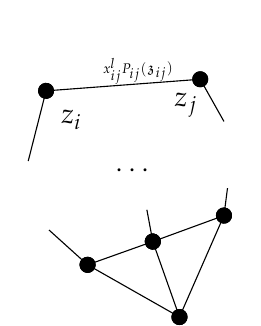
\begin{tikzpicture}[x=0.75pt,y=0.75pt,yscale=-1,xscale=1]
%uncomment if require: \path (0,214); %set diagram left start at 0, and has height of 214

%Straight Lines [id:da5823024143210767]
\draw    (318.95,172.29) -- (306.1,135.94) ;
\draw [shift={(306.1,135.94)}, rotate = 250.52] [color={rgb, 255:red, 0; green, 0; blue, 0 }  ][fill={rgb, 255:red, 0; green, 0; blue, 0 }  ][line width=0.75]      (0, 0) circle [x radius= 3.35, y radius= 3.35]   ;
\draw [shift={(318.95,172.29)}, rotate = 250.52] [color={rgb, 255:red, 0; green, 0; blue, 0 }  ][fill={rgb, 255:red, 0; green, 0; blue, 0 }  ][line width=0.75]      (0, 0) circle [x radius= 3.35, y radius= 3.35]   ;
%Straight Lines [id:da8147858505316599]
\draw    (328.95,57.74) -- (254.67,63.33) ;
\draw [shift={(254.67,63.33)}, rotate = 175.7] [color={rgb, 255:red, 0; green, 0; blue, 0 }  ][fill={rgb, 255:red, 0; green, 0; blue, 0 }  ][line width=0.75]      (0, 0) circle [x radius= 3.35, y radius= 3.35]   ;
\draw [shift={(328.95,57.74)}, rotate = 175.7] [color={rgb, 255:red, 0; green, 0; blue, 0 }  ][fill={rgb, 255:red, 0; green, 0; blue, 0 }  ][line width=0.75]      (0, 0) circle [x radius= 3.35, y radius= 3.35]   ;
%Straight Lines [id:da07628695201790259]
\draw    (274.67,147.14) -- (306.1,135.94) ;
\draw [shift={(306.1,135.94)}, rotate = 340.37] [color={rgb, 255:red, 0; green, 0; blue, 0 }  ][fill={rgb, 255:red, 0; green, 0; blue, 0 }  ][line width=0.75]      (0, 0) circle [x radius= 3.35, y radius= 3.35]   ;
\draw [shift={(274.67,147.14)}, rotate = 340.37] [color={rgb, 255:red, 0; green, 0; blue, 0 }  ][fill={rgb, 255:red, 0; green, 0; blue, 0 }  ][line width=0.75]      (0, 0) circle [x radius= 3.35, y radius= 3.35]   ;
%Straight Lines [id:da19384431212872455]
\draw    (274.67,147.14) -- (318.95,172.29) ;
\draw [shift={(318.95,172.29)}, rotate = 29.59] [color={rgb, 255:red, 0; green, 0; blue, 0 }  ][fill={rgb, 255:red, 0; green, 0; blue, 0 }  ][line width=0.75]      (0, 0) circle [x radius= 3.35, y radius= 3.35]   ;
\draw [shift={(274.67,147.14)}, rotate = 29.59] [color={rgb, 255:red, 0; green, 0; blue, 0 }  ][fill={rgb, 255:red, 0; green, 0; blue, 0 }  ][line width=0.75]      (0, 0) circle [x radius= 3.35, y radius= 3.35]   ;
%Straight Lines [id:da6790651752661128]
\draw    (254.67,63.33) -- (246.08,97.12) ;
\draw [shift={(254.67,63.33)}, rotate = 104.26] [color={rgb, 255:red, 0; green, 0; blue, 0 }  ][fill={rgb, 255:red, 0; green, 0; blue, 0 }  ][line width=0.75]      (0, 0) circle [x radius= 3.35, y radius= 3.35]   ;
%Straight Lines [id:da9419467958720287]
\draw    (328.95,57.74) -- (340.38,78.07) ;
\draw [shift={(328.95,57.74)}, rotate = 60.66] [color={rgb, 255:red, 0; green, 0; blue, 0 }  ][fill={rgb, 255:red, 0; green, 0; blue, 0 }  ][line width=0.75]      (0, 0) circle [x radius= 3.35, y radius= 3.35]   ;
%Straight Lines [id:da5446816494299196]
\draw    (306.1,135.94) -- (340.38,123.4) ;
\draw [shift={(340.38,123.4)}, rotate = 339.91] [color={rgb, 255:red, 0; green, 0; blue, 0 }  ][fill={rgb, 255:red, 0; green, 0; blue, 0 }  ][line width=0.75]      (0, 0) circle [x radius= 3.35, y radius= 3.35]   ;
\draw [shift={(306.1,135.94)}, rotate = 339.91] [color={rgb, 255:red, 0; green, 0; blue, 0 }  ][fill={rgb, 255:red, 0; green, 0; blue, 0 }  ][line width=0.75]      (0, 0) circle [x radius= 3.35, y radius= 3.35]   ;
%Straight Lines [id:da5595647047388295]
\draw    (274.67,147.14) -- (256.1,130.38) ;
\draw [shift={(274.67,147.14)}, rotate = 222.07] [color={rgb, 255:red, 0; green, 0; blue, 0 }  ][fill={rgb, 255:red, 0; green, 0; blue, 0 }  ][line width=0.75]      (0, 0) circle [x radius= 3.35, y radius= 3.35]   ;
%Straight Lines [id:da8588411657017472]
\draw    (306.1,135.94) -- (303.24,120.6) ;
\draw [shift={(306.1,135.94)}, rotate = 259.45] [color={rgb, 255:red, 0; green, 0; blue, 0 }  ][fill={rgb, 255:red, 0; green, 0; blue, 0 }  ][line width=0.75]      (0, 0) circle [x radius= 3.35, y radius= 3.35]   ;
%Straight Lines [id:da103614605215544]
\draw    (340.38,123.4) -- (342.08,110.21) ;
\draw [shift={(340.38,123.4)}, rotate = 277.36] [color={rgb, 255:red, 0; green, 0; blue, 0 }  ][fill={rgb, 255:red, 0; green, 0; blue, 0 }  ][line width=0.75]      (0, 0) circle [x radius= 3.35, y radius= 3.35]   ;
%Straight Lines [id:da4242958639619645]
\draw    (318.95,172.29) -- (340.38,123.4) ;
\draw [shift={(340.38,123.4)}, rotate = 293.67] [color={rgb, 255:red, 0; green, 0; blue, 0 }  ][fill={rgb, 255:red, 0; green, 0; blue, 0 }  ][line width=0.75]      (0, 0) circle [x radius= 3.35, y radius= 3.35]   ;
\draw [shift={(318.95,172.29)}, rotate = 293.67] [color={rgb, 255:red, 0; green, 0; blue, 0 }  ][fill={rgb, 255:red, 0; green, 0; blue, 0 }  ][line width=0.75]      (0, 0) circle [x radius= 3.35, y radius= 3.35]   ;

% Text Node
\draw (315.1,63.11) node [anchor=north west][inner sep=0.75pt]    {$z_{j}{}$};
% Text Node
\draw (260.53,71.49) node [anchor=north west][inner sep=0.75pt]    {$z_{i}$};
% Text Node
\draw (286.48,97.71) node [anchor=north west][inner sep=0.75pt]    {$\cdots $};
% Text Node
\draw (280.78,46.54) node [anchor=north west][inner sep=0.75pt]  [font=\tiny,rotate=-359.06]  {$x_{ij}^{l} P_{ij}(\mathfrak{z}_{ij})$};


\end{tikzpicture}
  \caption{}\label{}
\end{figure}
\begin{proof}

Using Lemma \ref{IntegralXP}, we have
$$
x^l_{ij}P_{ij}(\mathfrak{z}_{ij})=-\partial_{\mathfrak{z}^l_{ij}}\int^1_0P_{ij}(r\mathfrak{z}_{ij})dr.
$$
Then
\begin{align*}
   \mu_{\{o,1,\dots, n\}}\left(W_{\Gamma}(\mathfrak{z}_{e})\cdot x^l_{ij}\right)  &=\mu_{\{o,1,\dots, n\}}\left(-\partial_{\mathfrak{z}^l_{ij}}\int^1_0W_{\Gamma}(\dots,r\mathfrak{z}_{ij},\dots)dr\right)  \\
   & =-\partial_{\mathfrak{z}^l_{ij}}\int^1_0\mu_{\{o,1,\dots, n\}}\left(W_{\Gamma}(\dots,r\mathfrak{z}_{ij},\dots)\right)dr\\
   &=-\partial_{\mathfrak{z}^l_{ij}}\int^1_0F(\lambda_1,\dots,\lambda_{n};\dots,r\mathfrak{z}_{ij},\dots)dr.
\end{align*}
\end{proof}


\begin{lem}\label{IntegralS}
  Suppose that we have a graph with vertices $\{o,1,\dots,n\}$ and $i,j\subset \{o,1,\dots,n\}$ such that $(i,j)\in E_{\Gamma}$. Let $\mu_{\{o,1,\dots, n\}}\left(\alpha\right)=F_{\alpha}(\lambda)$. Then
  $$
  \mu_{\{\star,\bullet\}}\circ \mu_{\{o,1,\dots, n\}}\left(\alpha\cdot x^l_{\star i}P_{\star j }\right)=\int^1_0 F_{\alpha}(\lambda_1,\dots,\lambda_i+(1-s_{\star})\lambda_{\star},\dots,\lambda_j+s_{\star}\lambda_{\star},\lambda_{n};\mathfrak{z}_e)\cdot s_{\star}\lambda^l_{\star}ds_{\star}
  $$
    $$
  \mu_{\{\star,\bullet\}}\circ \mu_{\{o,1,\dots, n\}}\left(\alpha\cdot x^l_{\star j}P_{\star i }\right)=\int^1_0 F_{\alpha}(\lambda_1,\dots,\lambda_i+(1-s_{\star})\lambda_{\star},\dots,\lambda_j+s_{\star}\lambda_{\star},\lambda_{n};\mathfrak{z}_e)\cdot(1-s_{\star})\lambda^l_{\star}ds_{\star}
  $$
  Similarly, if $\star$ is joint with $(o,i)\in E_{\Gamma}$, then
  $$
  \mu_{\{\star,\bullet\}}\circ \mu_{\{o,1,\dots, n\}}\left(\alpha\cdot x^l_{\star i}P_{\star o }\right)=\int^1_0 F_{\alpha}(\lambda_1,\dots,\lambda_i+(1-s_{\star})\lambda_{\star},\dots,\lambda_{n};\mathfrak{z}_e)\cdot s_{\star}\lambda^l_{\star}ds_{\star}
  $$
   $$
  \mu_{\{\star,\bullet\}}\circ \mu_{\{o,1,\dots, n\}}\left(\alpha\cdot x^l_{\star o}P_{\star i}\right)=\int^1_0 F_{\alpha}(\lambda_1,\dots,\lambda_i+(1-s_{\star})\lambda_{\star},\dots,\lambda_{n};\mathfrak{z}_e)\cdot(1-s_{\star})\lambda^l_{\star}ds_{\star}
  $$
  See Fig. \ref{TwoMultOperation} for an illustration of $\mu_{\{\star,\bullet\}}\circ \mu_{\{o,1,\dots, n\}}\left(\alpha\cdot x^l_{\star i}P_{\star j }\right)$.
\end{lem}
\begin{proof}
  Write
  $$
\mu_{\{o,1,\dots, n\}}\left(\alpha\right)=F_{\alpha}(\lambda)=\sum G(\lambda_i)H(\lambda_j).
  $$
  Then
  \begin{align*}
   &  \mu_{\{\star,\bullet\}}\circ \mu_{\{o,1,\dots, n\}}\left(\alpha\cdot x^l_{\star i}P_{\star j }\right)=  \mu_{\{\star,\bullet\}}\left(\sum G(\lambda_i-\partial_{z_{\star}})x^l_{\star\bullet}\cdot H(\lambda_j-\partial_{z_{\star}})P_{\star\bullet}\right)\\
     &=\mu_{\{\star,\bullet\}}\left(\int^1_0\sum G(\lambda_i-(1-s)\partial_{z_{\star}}) H(\lambda_j-s\partial_{z_{\star}})(-s\partial_{z^l_{\star}})P_{\star\bullet}ds\right)\quad \text{using Lemma \ref{IntegralXP}}\\
     &=\int^1_0\sum G(\lambda_i+(1-s)\lambda_{\star}) H(\lambda_j+s\lambda_{\star})(s\lambda^l_{\star})ds\\
     &=\int^1_0 F_{\alpha}(\lambda_1,\dots,\lambda_i+(1-s_{\star})\lambda_{\star},\dots,\lambda_j+s_{\star}\lambda_{\star},\lambda_{n};\mathfrak{z}_e)\cdot(s_{\star}\lambda^l_{\star})ds_{\star}.
  \end{align*}
\end{proof}
\begin{figure}[htp]
  \centering


\tikzset{every picture/.style={line width=0.75pt}} %set default line width to 0.75pt

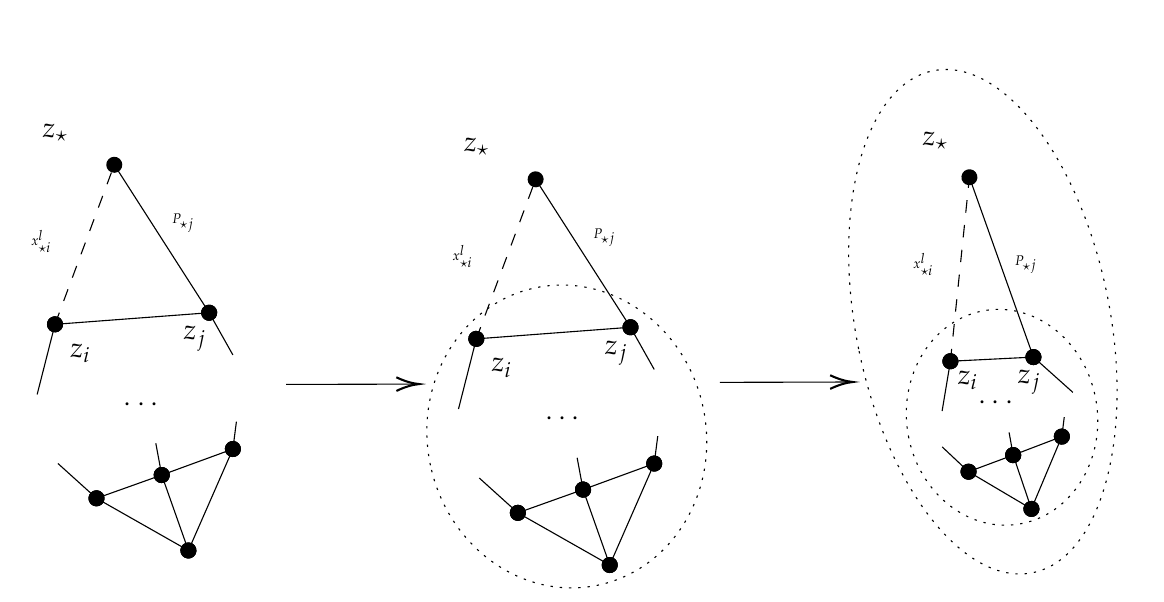
\begin{tikzpicture}[x=0.75pt,y=0.75pt,yscale=-1,xscale=1]
%uncomment if require: \path (0,300); %set diagram left start at 0, and has height of 300

%Straight Lines [id:da8577423121720247]
\draw  [dash pattern={on 4.5pt off 4.5pt}]  (60.67,131.04) -- (89.24,54.17) ;
\draw [shift={(89.24,54.17)}, rotate = 290.39] [color={rgb, 255:red, 0; green, 0; blue, 0 }  ][fill={rgb, 255:red, 0; green, 0; blue, 0 }  ][line width=0.75]      (0, 0) circle [x radius= 3.35, y radius= 3.35]   ;
\draw [shift={(60.67,131.04)}, rotate = 290.39] [color={rgb, 255:red, 0; green, 0; blue, 0 }  ][fill={rgb, 255:red, 0; green, 0; blue, 0 }  ][line width=0.75]      (0, 0) circle [x radius= 3.35, y radius= 3.35]   ;
%Straight Lines [id:da13261678783310793]
\draw    (134.95,125.45) -- (89.24,54.17) ;
\draw [shift={(134.95,125.45)}, rotate = 237.33] [color={rgb, 255:red, 0; green, 0; blue, 0 }  ][fill={rgb, 255:red, 0; green, 0; blue, 0 }  ][line width=0.75]      (0, 0) circle [x radius= 3.35, y radius= 3.35]   ;
%Straight Lines [id:da9919861590399197]
\draw    (124.95,240) -- (112.1,203.65) ;
\draw [shift={(112.1,203.65)}, rotate = 250.52] [color={rgb, 255:red, 0; green, 0; blue, 0 }  ][fill={rgb, 255:red, 0; green, 0; blue, 0 }  ][line width=0.75]      (0, 0) circle [x radius= 3.35, y radius= 3.35]   ;
\draw [shift={(124.95,240)}, rotate = 250.52] [color={rgb, 255:red, 0; green, 0; blue, 0 }  ][fill={rgb, 255:red, 0; green, 0; blue, 0 }  ][line width=0.75]      (0, 0) circle [x radius= 3.35, y radius= 3.35]   ;
%Straight Lines [id:da9722937517393717]
\draw    (134.95,125.45) -- (60.67,131.04) ;
\draw [shift={(60.67,131.04)}, rotate = 175.7] [color={rgb, 255:red, 0; green, 0; blue, 0 }  ][fill={rgb, 255:red, 0; green, 0; blue, 0 }  ][line width=0.75]      (0, 0) circle [x radius= 3.35, y radius= 3.35]   ;
\draw [shift={(134.95,125.45)}, rotate = 175.7] [color={rgb, 255:red, 0; green, 0; blue, 0 }  ][fill={rgb, 255:red, 0; green, 0; blue, 0 }  ][line width=0.75]      (0, 0) circle [x radius= 3.35, y radius= 3.35]   ;
%Straight Lines [id:da5603964973358293]
\draw    (80.67,214.86) -- (112.1,203.65) ;
\draw [shift={(112.1,203.65)}, rotate = 340.37] [color={rgb, 255:red, 0; green, 0; blue, 0 }  ][fill={rgb, 255:red, 0; green, 0; blue, 0 }  ][line width=0.75]      (0, 0) circle [x radius= 3.35, y radius= 3.35]   ;
\draw [shift={(80.67,214.86)}, rotate = 340.37] [color={rgb, 255:red, 0; green, 0; blue, 0 }  ][fill={rgb, 255:red, 0; green, 0; blue, 0 }  ][line width=0.75]      (0, 0) circle [x radius= 3.35, y radius= 3.35]   ;
%Straight Lines [id:da7092464873841009]
\draw    (80.67,214.86) -- (124.95,240) ;
\draw [shift={(124.95,240)}, rotate = 29.59] [color={rgb, 255:red, 0; green, 0; blue, 0 }  ][fill={rgb, 255:red, 0; green, 0; blue, 0 }  ][line width=0.75]      (0, 0) circle [x radius= 3.35, y radius= 3.35]   ;
\draw [shift={(80.67,214.86)}, rotate = 29.59] [color={rgb, 255:red, 0; green, 0; blue, 0 }  ][fill={rgb, 255:red, 0; green, 0; blue, 0 }  ][line width=0.75]      (0, 0) circle [x radius= 3.35, y radius= 3.35]   ;
%Straight Lines [id:da6671996787964425]
\draw    (60.67,131.04) -- (52.08,164.83) ;
\draw [shift={(60.67,131.04)}, rotate = 104.26] [color={rgb, 255:red, 0; green, 0; blue, 0 }  ][fill={rgb, 255:red, 0; green, 0; blue, 0 }  ][line width=0.75]      (0, 0) circle [x radius= 3.35, y radius= 3.35]   ;
%Straight Lines [id:da8921967722630684]
\draw    (134.95,125.45) -- (146.38,145.78) ;
\draw [shift={(134.95,125.45)}, rotate = 60.66] [color={rgb, 255:red, 0; green, 0; blue, 0 }  ][fill={rgb, 255:red, 0; green, 0; blue, 0 }  ][line width=0.75]      (0, 0) circle [x radius= 3.35, y radius= 3.35]   ;
%Straight Lines [id:da8599628892483835]
\draw    (112.1,203.65) -- (146.38,191.11) ;
\draw [shift={(146.38,191.11)}, rotate = 339.91] [color={rgb, 255:red, 0; green, 0; blue, 0 }  ][fill={rgb, 255:red, 0; green, 0; blue, 0 }  ][line width=0.75]      (0, 0) circle [x radius= 3.35, y radius= 3.35]   ;
\draw [shift={(112.1,203.65)}, rotate = 339.91] [color={rgb, 255:red, 0; green, 0; blue, 0 }  ][fill={rgb, 255:red, 0; green, 0; blue, 0 }  ][line width=0.75]      (0, 0) circle [x radius= 3.35, y radius= 3.35]   ;
%Straight Lines [id:da601234034482129]
\draw    (80.67,214.86) -- (62.1,198.09) ;
\draw [shift={(80.67,214.86)}, rotate = 222.07] [color={rgb, 255:red, 0; green, 0; blue, 0 }  ][fill={rgb, 255:red, 0; green, 0; blue, 0 }  ][line width=0.75]      (0, 0) circle [x radius= 3.35, y radius= 3.35]   ;
%Straight Lines [id:da7733669878066225]
\draw    (112.1,203.65) -- (109.24,188.31) ;
\draw [shift={(112.1,203.65)}, rotate = 259.45] [color={rgb, 255:red, 0; green, 0; blue, 0 }  ][fill={rgb, 255:red, 0; green, 0; blue, 0 }  ][line width=0.75]      (0, 0) circle [x radius= 3.35, y radius= 3.35]   ;
%Straight Lines [id:da22739188659656895]
\draw    (146.38,191.11) -- (148.08,177.92) ;
\draw [shift={(146.38,191.11)}, rotate = 277.36] [color={rgb, 255:red, 0; green, 0; blue, 0 }  ][fill={rgb, 255:red, 0; green, 0; blue, 0 }  ][line width=0.75]      (0, 0) circle [x radius= 3.35, y radius= 3.35]   ;
%Straight Lines [id:da28359362079359074]
\draw    (124.95,240) -- (146.38,191.11) ;
\draw [shift={(146.38,191.11)}, rotate = 293.67] [color={rgb, 255:red, 0; green, 0; blue, 0 }  ][fill={rgb, 255:red, 0; green, 0; blue, 0 }  ][line width=0.75]      (0, 0) circle [x radius= 3.35, y radius= 3.35]   ;
\draw [shift={(124.95,240)}, rotate = 293.67] [color={rgb, 255:red, 0; green, 0; blue, 0 }  ][fill={rgb, 255:red, 0; green, 0; blue, 0 }  ][line width=0.75]      (0, 0) circle [x radius= 3.35, y radius= 3.35]   ;
%Straight Lines [id:da44851088359116265]
\draw    (172,160) -- (234.08,159.83) ;
\draw [shift={(236.08,159.82)}, rotate = 179.84] [color={rgb, 255:red, 0; green, 0; blue, 0 }  ][line width=0.75]    (10.93,-3.29) .. controls (6.95,-1.4) and (3.31,-0.3) .. (0,0) .. controls (3.31,0.3) and (6.95,1.4) .. (10.93,3.29)   ;
%Straight Lines [id:da38480407885565926]
\draw  [dash pattern={on 4.5pt off 4.5pt}]  (263.67,138.04) -- (292.24,61.17) ;
\draw [shift={(292.24,61.17)}, rotate = 290.39] [color={rgb, 255:red, 0; green, 0; blue, 0 }  ][fill={rgb, 255:red, 0; green, 0; blue, 0 }  ][line width=0.75]      (0, 0) circle [x radius= 3.35, y radius= 3.35]   ;
\draw [shift={(263.67,138.04)}, rotate = 290.39] [color={rgb, 255:red, 0; green, 0; blue, 0 }  ][fill={rgb, 255:red, 0; green, 0; blue, 0 }  ][line width=0.75]      (0, 0) circle [x radius= 3.35, y radius= 3.35]   ;
%Straight Lines [id:da5307717551850348]
\draw    (337.95,132.45) -- (292.24,61.17) ;
\draw [shift={(337.95,132.45)}, rotate = 237.33] [color={rgb, 255:red, 0; green, 0; blue, 0 }  ][fill={rgb, 255:red, 0; green, 0; blue, 0 }  ][line width=0.75]      (0, 0) circle [x radius= 3.35, y radius= 3.35]   ;
%Straight Lines [id:da9413038592812624]
\draw    (327.95,247) -- (315.1,210.65) ;
\draw [shift={(315.1,210.65)}, rotate = 250.52] [color={rgb, 255:red, 0; green, 0; blue, 0 }  ][fill={rgb, 255:red, 0; green, 0; blue, 0 }  ][line width=0.75]      (0, 0) circle [x radius= 3.35, y radius= 3.35]   ;
\draw [shift={(327.95,247)}, rotate = 250.52] [color={rgb, 255:red, 0; green, 0; blue, 0 }  ][fill={rgb, 255:red, 0; green, 0; blue, 0 }  ][line width=0.75]      (0, 0) circle [x radius= 3.35, y radius= 3.35]   ;
%Straight Lines [id:da5150963015703387]
\draw    (337.95,132.45) -- (263.67,138.04) ;
\draw [shift={(263.67,138.04)}, rotate = 175.7] [color={rgb, 255:red, 0; green, 0; blue, 0 }  ][fill={rgb, 255:red, 0; green, 0; blue, 0 }  ][line width=0.75]      (0, 0) circle [x radius= 3.35, y radius= 3.35]   ;
\draw [shift={(337.95,132.45)}, rotate = 175.7] [color={rgb, 255:red, 0; green, 0; blue, 0 }  ][fill={rgb, 255:red, 0; green, 0; blue, 0 }  ][line width=0.75]      (0, 0) circle [x radius= 3.35, y radius= 3.35]   ;
%Straight Lines [id:da16397146641636162]
\draw    (283.67,221.86) -- (315.1,210.65) ;
\draw [shift={(315.1,210.65)}, rotate = 340.37] [color={rgb, 255:red, 0; green, 0; blue, 0 }  ][fill={rgb, 255:red, 0; green, 0; blue, 0 }  ][line width=0.75]      (0, 0) circle [x radius= 3.35, y radius= 3.35]   ;
\draw [shift={(283.67,221.86)}, rotate = 340.37] [color={rgb, 255:red, 0; green, 0; blue, 0 }  ][fill={rgb, 255:red, 0; green, 0; blue, 0 }  ][line width=0.75]      (0, 0) circle [x radius= 3.35, y radius= 3.35]   ;
%Straight Lines [id:da8143076274162886]
\draw    (283.67,221.86) -- (327.95,247) ;
\draw [shift={(327.95,247)}, rotate = 29.59] [color={rgb, 255:red, 0; green, 0; blue, 0 }  ][fill={rgb, 255:red, 0; green, 0; blue, 0 }  ][line width=0.75]      (0, 0) circle [x radius= 3.35, y radius= 3.35]   ;
\draw [shift={(283.67,221.86)}, rotate = 29.59] [color={rgb, 255:red, 0; green, 0; blue, 0 }  ][fill={rgb, 255:red, 0; green, 0; blue, 0 }  ][line width=0.75]      (0, 0) circle [x radius= 3.35, y radius= 3.35]   ;
%Straight Lines [id:da5832319766099261]
\draw    (263.67,138.04) -- (255.08,171.83) ;
\draw [shift={(263.67,138.04)}, rotate = 104.26] [color={rgb, 255:red, 0; green, 0; blue, 0 }  ][fill={rgb, 255:red, 0; green, 0; blue, 0 }  ][line width=0.75]      (0, 0) circle [x radius= 3.35, y radius= 3.35]   ;
%Straight Lines [id:da9359335501825665]
\draw    (337.95,132.45) -- (349.38,152.78) ;
\draw [shift={(337.95,132.45)}, rotate = 60.66] [color={rgb, 255:red, 0; green, 0; blue, 0 }  ][fill={rgb, 255:red, 0; green, 0; blue, 0 }  ][line width=0.75]      (0, 0) circle [x radius= 3.35, y radius= 3.35]   ;
%Straight Lines [id:da1782726456669681]
\draw    (315.1,210.65) -- (349.38,198.11) ;
\draw [shift={(349.38,198.11)}, rotate = 339.91] [color={rgb, 255:red, 0; green, 0; blue, 0 }  ][fill={rgb, 255:red, 0; green, 0; blue, 0 }  ][line width=0.75]      (0, 0) circle [x radius= 3.35, y radius= 3.35]   ;
\draw [shift={(315.1,210.65)}, rotate = 339.91] [color={rgb, 255:red, 0; green, 0; blue, 0 }  ][fill={rgb, 255:red, 0; green, 0; blue, 0 }  ][line width=0.75]      (0, 0) circle [x radius= 3.35, y radius= 3.35]   ;
%Straight Lines [id:da7217720127600564]
\draw    (283.67,221.86) -- (265.1,205.09) ;
\draw [shift={(283.67,221.86)}, rotate = 222.07] [color={rgb, 255:red, 0; green, 0; blue, 0 }  ][fill={rgb, 255:red, 0; green, 0; blue, 0 }  ][line width=0.75]      (0, 0) circle [x radius= 3.35, y radius= 3.35]   ;
%Straight Lines [id:da9726191077362507]
\draw    (315.1,210.65) -- (312.24,195.31) ;
\draw [shift={(315.1,210.65)}, rotate = 259.45] [color={rgb, 255:red, 0; green, 0; blue, 0 }  ][fill={rgb, 255:red, 0; green, 0; blue, 0 }  ][line width=0.75]      (0, 0) circle [x radius= 3.35, y radius= 3.35]   ;
%Straight Lines [id:da9228840677417147]
\draw    (349.38,198.11) -- (351.08,184.92) ;
\draw [shift={(349.38,198.11)}, rotate = 277.36] [color={rgb, 255:red, 0; green, 0; blue, 0 }  ][fill={rgb, 255:red, 0; green, 0; blue, 0 }  ][line width=0.75]      (0, 0) circle [x radius= 3.35, y radius= 3.35]   ;
%Straight Lines [id:da7187239691883223]
\draw    (327.95,247) -- (349.38,198.11) ;
\draw [shift={(349.38,198.11)}, rotate = 293.67] [color={rgb, 255:red, 0; green, 0; blue, 0 }  ][fill={rgb, 255:red, 0; green, 0; blue, 0 }  ][line width=0.75]      (0, 0) circle [x radius= 3.35, y radius= 3.35]   ;
\draw [shift={(327.95,247)}, rotate = 293.67] [color={rgb, 255:red, 0; green, 0; blue, 0 }  ][fill={rgb, 255:red, 0; green, 0; blue, 0 }  ][line width=0.75]      (0, 0) circle [x radius= 3.35, y radius= 3.35]   ;
%Shape: Ellipse [id:dp4777570083321534]
\draw  [dash pattern={on 0.84pt off 2.51pt}] (241.56,198.94) .. controls (233.21,159.38) and (255.86,121.1) .. (292.14,113.44) .. controls (328.43,105.78) and (364.61,131.64) .. (372.96,171.2) .. controls (381.31,210.76) and (358.67,249.03) .. (322.38,256.69) .. controls (286.1,264.35) and (249.91,238.49) .. (241.56,198.94) -- cycle ;
%Straight Lines [id:da2717921113507169]
\draw    (381,159) -- (443.08,158.83) ;
\draw [shift={(445.08,158.82)}, rotate = 179.84] [color={rgb, 255:red, 0; green, 0; blue, 0 }  ][line width=0.75]    (10.93,-3.29) .. controls (6.95,-1.4) and (3.31,-0.3) .. (0,0) .. controls (3.31,0.3) and (6.95,1.4) .. (10.93,3.29)   ;
%Straight Lines [id:da9369417437849918]
\draw  [dash pattern={on 4.5pt off 4.5pt}]  (492.08,148.82) -- (501.24,60.17) ;
\draw [shift={(501.24,60.17)}, rotate = 275.9] [color={rgb, 255:red, 0; green, 0; blue, 0 }  ][fill={rgb, 255:red, 0; green, 0; blue, 0 }  ][line width=0.75]      (0, 0) circle [x radius= 3.35, y radius= 3.35]   ;
\draw [shift={(492.08,148.82)}, rotate = 275.9] [color={rgb, 255:red, 0; green, 0; blue, 0 }  ][fill={rgb, 255:red, 0; green, 0; blue, 0 }  ][line width=0.75]      (0, 0) circle [x radius= 3.35, y radius= 3.35]   ;
%Straight Lines [id:da9853072568986168]
\draw    (532.08,146.82) -- (501.24,60.17) ;
\draw [shift={(532.08,146.82)}, rotate = 250.41] [color={rgb, 255:red, 0; green, 0; blue, 0 }  ][fill={rgb, 255:red, 0; green, 0; blue, 0 }  ][line width=0.75]      (0, 0) circle [x radius= 3.35, y radius= 3.35]   ;
%Straight Lines [id:da41602927139069523]
\draw    (531.11,219.96) -- (522.32,194.05) ;
\draw [shift={(522.32,194.05)}, rotate = 251.25] [color={rgb, 255:red, 0; green, 0; blue, 0 }  ][fill={rgb, 255:red, 0; green, 0; blue, 0 }  ][line width=0.75]      (0, 0) circle [x radius= 3.35, y radius= 3.35]   ;
\draw [shift={(531.11,219.96)}, rotate = 251.25] [color={rgb, 255:red, 0; green, 0; blue, 0 }  ][fill={rgb, 255:red, 0; green, 0; blue, 0 }  ][line width=0.75]      (0, 0) circle [x radius= 3.35, y radius= 3.35]   ;
%Straight Lines [id:da4586830007929794]
\draw    (532.08,146.82) -- (492.08,148.82) ;
\draw [shift={(492.08,148.82)}, rotate = 177.14] [color={rgb, 255:red, 0; green, 0; blue, 0 }  ][fill={rgb, 255:red, 0; green, 0; blue, 0 }  ][line width=0.75]      (0, 0) circle [x radius= 3.35, y radius= 3.35]   ;
\draw [shift={(532.08,146.82)}, rotate = 177.14] [color={rgb, 255:red, 0; green, 0; blue, 0 }  ][fill={rgb, 255:red, 0; green, 0; blue, 0 }  ][line width=0.75]      (0, 0) circle [x radius= 3.35, y radius= 3.35]   ;
%Straight Lines [id:da8800919049561395]
\draw    (500.82,202.04) -- (522.32,194.05) ;
\draw [shift={(522.32,194.05)}, rotate = 339.62] [color={rgb, 255:red, 0; green, 0; blue, 0 }  ][fill={rgb, 255:red, 0; green, 0; blue, 0 }  ][line width=0.75]      (0, 0) circle [x radius= 3.35, y radius= 3.35]   ;
\draw [shift={(500.82,202.04)}, rotate = 339.62] [color={rgb, 255:red, 0; green, 0; blue, 0 }  ][fill={rgb, 255:red, 0; green, 0; blue, 0 }  ][line width=0.75]      (0, 0) circle [x radius= 3.35, y radius= 3.35]   ;
%Straight Lines [id:da09222954685831342]
\draw    (500.82,202.04) -- (531.11,219.96) ;
\draw [shift={(531.11,219.96)}, rotate = 30.61] [color={rgb, 255:red, 0; green, 0; blue, 0 }  ][fill={rgb, 255:red, 0; green, 0; blue, 0 }  ][line width=0.75]      (0, 0) circle [x radius= 3.35, y radius= 3.35]   ;
\draw [shift={(500.82,202.04)}, rotate = 30.61] [color={rgb, 255:red, 0; green, 0; blue, 0 }  ][fill={rgb, 255:red, 0; green, 0; blue, 0 }  ][line width=0.75]      (0, 0) circle [x radius= 3.35, y radius= 3.35]   ;
%Straight Lines [id:da4563450226607171]
\draw    (492.08,148.82) -- (488.08,172.82) ;
\draw [shift={(492.08,148.82)}, rotate = 99.46] [color={rgb, 255:red, 0; green, 0; blue, 0 }  ][fill={rgb, 255:red, 0; green, 0; blue, 0 }  ][line width=0.75]      (0, 0) circle [x radius= 3.35, y radius= 3.35]   ;
%Straight Lines [id:da20087686932634408]
\draw    (532.08,146.82) -- (551.08,163.82) ;
\draw [shift={(532.08,146.82)}, rotate = 41.82] [color={rgb, 255:red, 0; green, 0; blue, 0 }  ][fill={rgb, 255:red, 0; green, 0; blue, 0 }  ][line width=0.75]      (0, 0) circle [x radius= 3.35, y radius= 3.35]   ;
%Straight Lines [id:da9710477288628783]
\draw    (522.32,194.05) -- (545.77,185.11) ;
\draw [shift={(545.77,185.11)}, rotate = 339.14] [color={rgb, 255:red, 0; green, 0; blue, 0 }  ][fill={rgb, 255:red, 0; green, 0; blue, 0 }  ][line width=0.75]      (0, 0) circle [x radius= 3.35, y radius= 3.35]   ;
\draw [shift={(522.32,194.05)}, rotate = 339.14] [color={rgb, 255:red, 0; green, 0; blue, 0 }  ][fill={rgb, 255:red, 0; green, 0; blue, 0 }  ][line width=0.75]      (0, 0) circle [x radius= 3.35, y radius= 3.35]   ;
%Straight Lines [id:da22424434990223552]
\draw    (500.82,202.04) -- (488.12,190.09) ;
\draw [shift={(500.82,202.04)}, rotate = 223.24] [color={rgb, 255:red, 0; green, 0; blue, 0 }  ][fill={rgb, 255:red, 0; green, 0; blue, 0 }  ][line width=0.75]      (0, 0) circle [x radius= 3.35, y radius= 3.35]   ;
%Straight Lines [id:da9762485288475353]
\draw    (522.32,194.05) -- (520.36,183.12) ;
\draw [shift={(522.32,194.05)}, rotate = 259.86] [color={rgb, 255:red, 0; green, 0; blue, 0 }  ][fill={rgb, 255:red, 0; green, 0; blue, 0 }  ][line width=0.75]      (0, 0) circle [x radius= 3.35, y radius= 3.35]   ;
%Straight Lines [id:da3615614902452422]
\draw    (545.77,185.11) -- (546.93,175.72) ;
\draw [shift={(545.77,185.11)}, rotate = 277.07] [color={rgb, 255:red, 0; green, 0; blue, 0 }  ][fill={rgb, 255:red, 0; green, 0; blue, 0 }  ][line width=0.75]      (0, 0) circle [x radius= 3.35, y radius= 3.35]   ;
%Straight Lines [id:da13050800750452307]
\draw    (531.11,219.96) -- (545.77,185.11) ;
\draw [shift={(545.77,185.11)}, rotate = 292.81] [color={rgb, 255:red, 0; green, 0; blue, 0 }  ][fill={rgb, 255:red, 0; green, 0; blue, 0 }  ][line width=0.75]      (0, 0) circle [x radius= 3.35, y radius= 3.35]   ;
\draw [shift={(531.11,219.96)}, rotate = 292.81] [color={rgb, 255:red, 0; green, 0; blue, 0 }  ][fill={rgb, 255:red, 0; green, 0; blue, 0 }  ][line width=0.75]      (0, 0) circle [x radius= 3.35, y radius= 3.35]   ;
%Shape: Ellipse [id:dp8788676993480489]
\draw  [dash pattern={on 0.84pt off 2.51pt}] (472.01,185.7) .. controls (466.3,157.52) and (481.8,130.24) .. (506.62,124.78) .. controls (531.44,119.33) and (556.19,137.75) .. (561.9,165.94) .. controls (567.61,194.13) and (552.12,221.41) .. (527.3,226.86) .. controls (502.47,232.32) and (477.72,213.89) .. (472.01,185.7) -- cycle ;
%Shape: Ellipse [id:dp25977476782180076]
\draw  [dash pattern={on 0.84pt off 2.51pt}] (447.88,142.94) .. controls (434.37,76.22) and (450.2,16.24) .. (483.25,8.98) .. controls (516.3,1.71) and (554.04,49.91) .. (567.55,116.63) .. controls (581.07,183.35) and (565.23,243.32) .. (532.19,250.59) .. controls (499.14,257.85) and (461.4,209.66) .. (447.88,142.94) -- cycle ;

% Text Node
\draw (53.19,33.11) node [anchor=north west][inner sep=0.75pt]    {$z_{\star }$};
% Text Node
\draw (121.1,130.82) node [anchor=north west][inner sep=0.75pt]    {$z_{j}{}$};
% Text Node
\draw (66.53,139.2) node [anchor=north west][inner sep=0.75pt]    {$z_{i}$};
% Text Node
\draw (92.48,165.42) node [anchor=north west][inner sep=0.75pt]    {$\cdots $};
% Text Node
\draw (47.78,84.62) node [anchor=north west][inner sep=0.75pt]  [font=\tiny,rotate=-359.06]  {$x_{\star i}^{l}$};
% Text Node
\draw (115.78,76.62) node [anchor=north west][inner sep=0.75pt]  [font=\tiny,rotate=-359.06]  {$P_{\star j}$};
% Text Node
\draw (256.19,40.11) node [anchor=north west][inner sep=0.75pt]    {$z_{\star }$};
% Text Node
\draw (324.1,137.82) node [anchor=north west][inner sep=0.75pt]    {$z_{j}{}$};
% Text Node
\draw (269.53,146.2) node [anchor=north west][inner sep=0.75pt]    {$z_{i}$};
% Text Node
\draw (295.48,172.42) node [anchor=north west][inner sep=0.75pt]    {$\cdots $};
% Text Node
\draw (250.78,91.62) node [anchor=north west][inner sep=0.75pt]  [font=\tiny,rotate=-359.06]  {$x_{\star i}^{l}$};
% Text Node
\draw (318.78,83.62) node [anchor=north west][inner sep=0.75pt]  [font=\tiny,rotate=-359.06]  {$P_{\star j}$};
% Text Node
\draw (477.19,37.11) node [anchor=north west][inner sep=0.75pt]    {$z_{\star }$};
% Text Node
\draw (523.1,151.82) node [anchor=north west][inner sep=0.75pt]    {$z_{j}{}$};
% Text Node
\draw (494.08,152.22) node [anchor=north west][inner sep=0.75pt]    {$z_{i}$};
% Text Node
\draw (504.31,164.63) node [anchor=north west][inner sep=0.75pt]    {$\cdots $};
% Text Node
\draw (472.78,95.62) node [anchor=north west][inner sep=0.75pt]  [font=\tiny,rotate=-359.06]  {$x_{\star i}^{l}$};
% Text Node
\draw (521.78,96.62) node [anchor=north west][inner sep=0.75pt]  [font=\tiny,rotate=-359.06]  {$P_{\star j}$};


\end{tikzpicture}
  \caption{$\mu_{\{\star,\bullet\}}\circ \mu_{\{o,1,\dots, n\}}\left(\alpha\cdot x^l_{\star i}P_{\star j }\right)$}\label{TwoMultOperation}
\end{figure}
\iffalse
\begin{figure}[htp]
  \centering


\tikzset{every picture/.style={line width=0.75pt}} %set default line width to 0.75pt

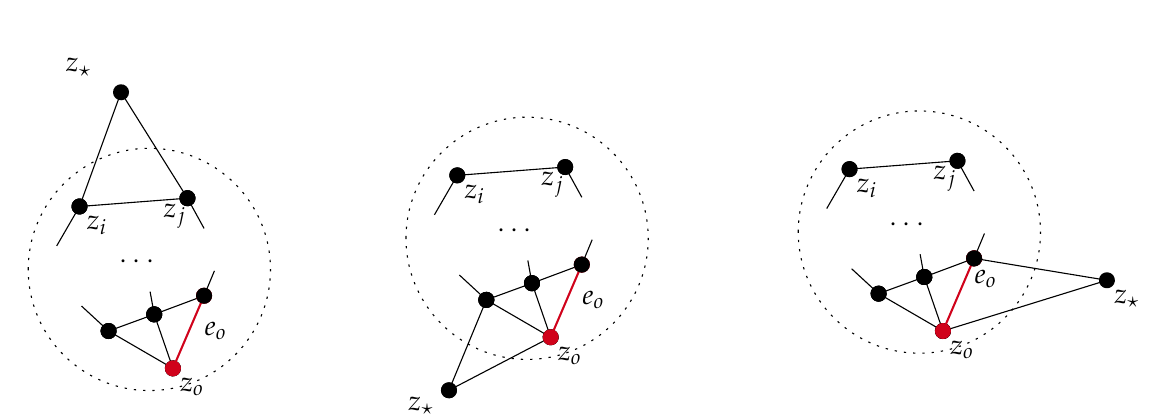
\begin{tikzpicture}[x=0.75pt,y=0.75pt,yscale=-1,xscale=1]
%uncomment if require: \path (0,283); %set diagram left start at 0, and has height of 283

%Shape: Circle [id:dp8083702044501739]
\draw  [dash pattern={on 0.84pt off 2.51pt}] (45.37,133.27) .. controls (45.37,101.05) and (71.5,74.92) .. (103.73,74.92) .. controls (135.95,74.92) and (162.08,101.05) .. (162.08,133.27) .. controls (162.08,165.5) and (135.95,191.63) .. (103.73,191.63) .. controls (71.5,191.63) and (45.37,165.5) .. (45.37,133.27) -- cycle ;
%Straight Lines [id:da41116817354603885]
\draw    (70.08,102.95) -- (90.08,47.92) ;
\draw [shift={(90.08,47.92)}, rotate = 289.98] [color={rgb, 255:red, 0; green, 0; blue, 0 }  ][fill={rgb, 255:red, 0; green, 0; blue, 0 }  ][line width=0.75]      (0, 0) circle [x radius= 3.35, y radius= 3.35]   ;
\draw [shift={(70.08,102.95)}, rotate = 289.98] [color={rgb, 255:red, 0; green, 0; blue, 0 }  ][fill={rgb, 255:red, 0; green, 0; blue, 0 }  ][line width=0.75]      (0, 0) circle [x radius= 3.35, y radius= 3.35]   ;
%Straight Lines [id:da34277569523600615]
\draw    (122.08,98.95) -- (90.08,47.92) ;
\draw [shift={(122.08,98.95)}, rotate = 237.91] [color={rgb, 255:red, 0; green, 0; blue, 0 }  ][fill={rgb, 255:red, 0; green, 0; blue, 0 }  ][line width=0.75]      (0, 0) circle [x radius= 3.35, y radius= 3.35]   ;
%Straight Lines [id:da5089975102649578]
\draw    (115.08,180.95) -- (106.08,154.92) ;
\draw [shift={(106.08,154.92)}, rotate = 250.92] [color={rgb, 255:red, 0; green, 0; blue, 0 }  ][fill={rgb, 255:red, 0; green, 0; blue, 0 }  ][line width=0.75]      (0, 0) circle [x radius= 3.35, y radius= 3.35]   ;
\draw [shift={(115.08,180.95)}, rotate = 250.92] [color={rgb, 255:red, 0; green, 0; blue, 0 }  ][fill={rgb, 255:red, 0; green, 0; blue, 0 }  ][line width=0.75]      (0, 0) circle [x radius= 3.35, y radius= 3.35]   ;
%Straight Lines [id:da5223764515960876]
\draw    (122.08,98.95) -- (70.08,102.95) ;
\draw [shift={(70.08,102.95)}, rotate = 175.6] [color={rgb, 255:red, 0; green, 0; blue, 0 }  ][fill={rgb, 255:red, 0; green, 0; blue, 0 }  ][line width=0.75]      (0, 0) circle [x radius= 3.35, y radius= 3.35]   ;
\draw [shift={(122.08,98.95)}, rotate = 175.6] [color={rgb, 255:red, 0; green, 0; blue, 0 }  ][fill={rgb, 255:red, 0; green, 0; blue, 0 }  ][line width=0.75]      (0, 0) circle [x radius= 3.35, y radius= 3.35]   ;
%Straight Lines [id:da3133816919828669]
\draw    (84.08,162.95) -- (106.08,154.92) ;
\draw [shift={(106.08,154.92)}, rotate = 339.96] [color={rgb, 255:red, 0; green, 0; blue, 0 }  ][fill={rgb, 255:red, 0; green, 0; blue, 0 }  ][line width=0.75]      (0, 0) circle [x radius= 3.35, y radius= 3.35]   ;
\draw [shift={(84.08,162.95)}, rotate = 339.96] [color={rgb, 255:red, 0; green, 0; blue, 0 }  ][fill={rgb, 255:red, 0; green, 0; blue, 0 }  ][line width=0.75]      (0, 0) circle [x radius= 3.35, y radius= 3.35]   ;
%Straight Lines [id:da2989742473880517]
\draw    (84.08,162.95) -- (115.08,180.95) ;
\draw [shift={(115.08,180.95)}, rotate = 30.14] [color={rgb, 255:red, 0; green, 0; blue, 0 }  ][fill={rgb, 255:red, 0; green, 0; blue, 0 }  ][line width=0.75]      (0, 0) circle [x radius= 3.35, y radius= 3.35]   ;
\draw [shift={(84.08,162.95)}, rotate = 30.14] [color={rgb, 255:red, 0; green, 0; blue, 0 }  ][fill={rgb, 255:red, 0; green, 0; blue, 0 }  ][line width=0.75]      (0, 0) circle [x radius= 3.35, y radius= 3.35]   ;
%Straight Lines [id:da13987264129177768]
\draw    (70.08,102.95) -- (59.08,121.95) ;
\draw [shift={(70.08,102.95)}, rotate = 120.07] [color={rgb, 255:red, 0; green, 0; blue, 0 }  ][fill={rgb, 255:red, 0; green, 0; blue, 0 }  ][line width=0.75]      (0, 0) circle [x radius= 3.35, y radius= 3.35]   ;
%Straight Lines [id:da4882856746367197]
\draw    (122.08,98.95) -- (130.08,113.5) ;
\draw [shift={(122.08,98.95)}, rotate = 61.21] [color={rgb, 255:red, 0; green, 0; blue, 0 }  ][fill={rgb, 255:red, 0; green, 0; blue, 0 }  ][line width=0.75]      (0, 0) circle [x radius= 3.35, y radius= 3.35]   ;
%Straight Lines [id:da39399358681544383]
\draw    (106.08,154.92) -- (130.08,145.95) ;
\draw [shift={(130.08,145.95)}, rotate = 339.49] [color={rgb, 255:red, 0; green, 0; blue, 0 }  ][fill={rgb, 255:red, 0; green, 0; blue, 0 }  ][line width=0.75]      (0, 0) circle [x radius= 3.35, y radius= 3.35]   ;
\draw [shift={(106.08,154.92)}, rotate = 339.49] [color={rgb, 255:red, 0; green, 0; blue, 0 }  ][fill={rgb, 255:red, 0; green, 0; blue, 0 }  ][line width=0.75]      (0, 0) circle [x radius= 3.35, y radius= 3.35]   ;
%Straight Lines [id:da021943993347968815]
\draw [color={rgb, 255:red, 208; green, 2; blue, 27 }  ,draw opacity=1 ][line width=0.75]    (115.08,180.95) -- (130.08,145.95) ;
\draw [shift={(130.08,145.95)}, rotate = 293.2] [color={rgb, 255:red, 208; green, 2; blue, 27 }  ,draw opacity=1 ][fill={rgb, 255:red, 208; green, 2; blue, 27 }  ,fill opacity=1 ][line width=0.75]      (0, 0) circle [x radius= 3.35, y radius= 3.35]   ;
\draw [shift={(115.08,180.95)}, rotate = 293.2] [color={rgb, 255:red, 208; green, 2; blue, 27 }  ,draw opacity=1 ][fill={rgb, 255:red, 208; green, 2; blue, 27 }  ,fill opacity=1 ][line width=0.75]      (0, 0) circle [x radius= 3.35, y radius= 3.35]   ;
%Straight Lines [id:da29682217038769654]
\draw    (84.08,162.95) -- (71.08,150.95) ;
\draw [shift={(84.08,162.95)}, rotate = 222.71] [color={rgb, 255:red, 0; green, 0; blue, 0 }  ][fill={rgb, 255:red, 0; green, 0; blue, 0 }  ][line width=0.75]      (0, 0) circle [x radius= 3.35, y radius= 3.35]   ;
%Straight Lines [id:da5496072141611632]
\draw    (106.08,154.92) -- (104.08,143.95) ;
\draw [shift={(106.08,154.92)}, rotate = 259.67] [color={rgb, 255:red, 0; green, 0; blue, 0 }  ][fill={rgb, 255:red, 0; green, 0; blue, 0 }  ][line width=0.75]      (0, 0) circle [x radius= 3.35, y radius= 3.35]   ;
%Straight Lines [id:da5967119205460225]
\draw    (130.08,145.95) -- (135.08,133.95) ;
\draw [shift={(130.08,145.95)}, rotate = 292.62] [color={rgb, 255:red, 0; green, 0; blue, 0 }  ][fill={rgb, 255:red, 0; green, 0; blue, 0 }  ][line width=0.75]      (0, 0) circle [x radius= 3.35, y radius= 3.35]   ;
%Shape: Circle [id:dp50413822479079]
\draw  [dash pattern={on 0.84pt off 2.51pt}] (227.37,118.27) .. controls (227.37,86.05) and (253.5,59.92) .. (285.73,59.92) .. controls (317.95,59.92) and (344.08,86.05) .. (344.08,118.27) .. controls (344.08,150.5) and (317.95,176.63) .. (285.73,176.63) .. controls (253.5,176.63) and (227.37,150.5) .. (227.37,118.27) -- cycle ;
%Straight Lines [id:da1648119557380343]
\draw    (266.08,147.95) -- (248.08,191.5) ;
\draw [shift={(248.08,191.5)}, rotate = 112.45] [color={rgb, 255:red, 0; green, 0; blue, 0 }  ][fill={rgb, 255:red, 0; green, 0; blue, 0 }  ][line width=0.75]      (0, 0) circle [x radius= 3.35, y radius= 3.35]   ;
\draw [shift={(266.08,147.95)}, rotate = 112.45] [color={rgb, 255:red, 0; green, 0; blue, 0 }  ][fill={rgb, 255:red, 0; green, 0; blue, 0 }  ][line width=0.75]      (0, 0) circle [x radius= 3.35, y radius= 3.35]   ;
%Straight Lines [id:da6236095673422983]
\draw    (248.08,191.5) -- (297.08,165.95) ;
\draw [shift={(248.08,191.5)}, rotate = 332.46] [color={rgb, 255:red, 0; green, 0; blue, 0 }  ][fill={rgb, 255:red, 0; green, 0; blue, 0 }  ][line width=0.75]      (0, 0) circle [x radius= 3.35, y radius= 3.35]   ;
%Straight Lines [id:da7220199169895192]
\draw    (297.08,165.95) -- (288.08,139.92) ;
\draw [shift={(288.08,139.92)}, rotate = 250.92] [color={rgb, 255:red, 0; green, 0; blue, 0 }  ][fill={rgb, 255:red, 0; green, 0; blue, 0 }  ][line width=0.75]      (0, 0) circle [x radius= 3.35, y radius= 3.35]   ;
\draw [shift={(297.08,165.95)}, rotate = 250.92] [color={rgb, 255:red, 0; green, 0; blue, 0 }  ][fill={rgb, 255:red, 0; green, 0; blue, 0 }  ][line width=0.75]      (0, 0) circle [x radius= 3.35, y radius= 3.35]   ;
%Straight Lines [id:da7995796109380549]
\draw    (304.08,83.95) -- (252.08,87.95) ;
\draw [shift={(252.08,87.95)}, rotate = 175.6] [color={rgb, 255:red, 0; green, 0; blue, 0 }  ][fill={rgb, 255:red, 0; green, 0; blue, 0 }  ][line width=0.75]      (0, 0) circle [x radius= 3.35, y radius= 3.35]   ;
\draw [shift={(304.08,83.95)}, rotate = 175.6] [color={rgb, 255:red, 0; green, 0; blue, 0 }  ][fill={rgb, 255:red, 0; green, 0; blue, 0 }  ][line width=0.75]      (0, 0) circle [x radius= 3.35, y radius= 3.35]   ;
%Straight Lines [id:da42111529394151104]
\draw    (266.08,147.95) -- (288.08,139.92) ;
\draw [shift={(288.08,139.92)}, rotate = 339.96] [color={rgb, 255:red, 0; green, 0; blue, 0 }  ][fill={rgb, 255:red, 0; green, 0; blue, 0 }  ][line width=0.75]      (0, 0) circle [x radius= 3.35, y radius= 3.35]   ;
\draw [shift={(266.08,147.95)}, rotate = 339.96] [color={rgb, 255:red, 0; green, 0; blue, 0 }  ][fill={rgb, 255:red, 0; green, 0; blue, 0 }  ][line width=0.75]      (0, 0) circle [x radius= 3.35, y radius= 3.35]   ;
%Straight Lines [id:da7027578449791063]
\draw    (266.08,147.95) -- (297.08,165.95) ;
\draw [shift={(297.08,165.95)}, rotate = 30.14] [color={rgb, 255:red, 0; green, 0; blue, 0 }  ][fill={rgb, 255:red, 0; green, 0; blue, 0 }  ][line width=0.75]      (0, 0) circle [x radius= 3.35, y radius= 3.35]   ;
\draw [shift={(266.08,147.95)}, rotate = 30.14] [color={rgb, 255:red, 0; green, 0; blue, 0 }  ][fill={rgb, 255:red, 0; green, 0; blue, 0 }  ][line width=0.75]      (0, 0) circle [x radius= 3.35, y radius= 3.35]   ;
%Straight Lines [id:da809651028097278]
\draw    (252.08,87.95) -- (241.08,106.95) ;
\draw [shift={(252.08,87.95)}, rotate = 120.07] [color={rgb, 255:red, 0; green, 0; blue, 0 }  ][fill={rgb, 255:red, 0; green, 0; blue, 0 }  ][line width=0.75]      (0, 0) circle [x radius= 3.35, y radius= 3.35]   ;
%Straight Lines [id:da44375980516038616]
\draw    (304.08,83.95) -- (312.08,98.5) ;
\draw [shift={(304.08,83.95)}, rotate = 61.21] [color={rgb, 255:red, 0; green, 0; blue, 0 }  ][fill={rgb, 255:red, 0; green, 0; blue, 0 }  ][line width=0.75]      (0, 0) circle [x radius= 3.35, y radius= 3.35]   ;
%Straight Lines [id:da1578506933143189]
\draw    (288.08,139.92) -- (312.08,130.95) ;
\draw [shift={(312.08,130.95)}, rotate = 339.49] [color={rgb, 255:red, 0; green, 0; blue, 0 }  ][fill={rgb, 255:red, 0; green, 0; blue, 0 }  ][line width=0.75]      (0, 0) circle [x radius= 3.35, y radius= 3.35]   ;
\draw [shift={(288.08,139.92)}, rotate = 339.49] [color={rgb, 255:red, 0; green, 0; blue, 0 }  ][fill={rgb, 255:red, 0; green, 0; blue, 0 }  ][line width=0.75]      (0, 0) circle [x radius= 3.35, y radius= 3.35]   ;
%Straight Lines [id:da2978924613859981]
\draw [color={rgb, 255:red, 208; green, 2; blue, 27 }  ,draw opacity=1 ][line width=0.75]    (297.08,165.95) -- (312.08,130.95) ;
\draw [shift={(312.08,130.95)}, rotate = 293.2] [color={rgb, 255:red, 208; green, 2; blue, 27 }  ,draw opacity=1 ][fill={rgb, 255:red, 208; green, 2; blue, 27 }  ,fill opacity=1 ][line width=0.75]      (0, 0) circle [x radius= 3.35, y radius= 3.35]   ;
\draw [shift={(297.08,165.95)}, rotate = 293.2] [color={rgb, 255:red, 208; green, 2; blue, 27 }  ,draw opacity=1 ][fill={rgb, 255:red, 208; green, 2; blue, 27 }  ,fill opacity=1 ][line width=0.75]      (0, 0) circle [x radius= 3.35, y radius= 3.35]   ;
%Straight Lines [id:da751353817269335]
\draw    (266.08,147.95) -- (253.08,135.95) ;
\draw [shift={(266.08,147.95)}, rotate = 222.71] [color={rgb, 255:red, 0; green, 0; blue, 0 }  ][fill={rgb, 255:red, 0; green, 0; blue, 0 }  ][line width=0.75]      (0, 0) circle [x radius= 3.35, y radius= 3.35]   ;
%Straight Lines [id:da7004857357994263]
\draw    (288.08,139.92) -- (286.08,128.95) ;
\draw [shift={(288.08,139.92)}, rotate = 259.67] [color={rgb, 255:red, 0; green, 0; blue, 0 }  ][fill={rgb, 255:red, 0; green, 0; blue, 0 }  ][line width=0.75]      (0, 0) circle [x radius= 3.35, y radius= 3.35]   ;
%Straight Lines [id:da8899129111575641]
\draw    (312.08,130.95) -- (317.08,118.95) ;
\draw [shift={(312.08,130.95)}, rotate = 292.62] [color={rgb, 255:red, 0; green, 0; blue, 0 }  ][fill={rgb, 255:red, 0; green, 0; blue, 0 }  ][line width=0.75]      (0, 0) circle [x radius= 3.35, y radius= 3.35]   ;
%Shape: Circle [id:dp27756615495394454]
\draw  [dash pattern={on 0.84pt off 2.51pt}] (416.37,115.27) .. controls (416.37,83.05) and (442.5,56.92) .. (474.73,56.92) .. controls (506.95,56.92) and (533.08,83.05) .. (533.08,115.27) .. controls (533.08,147.5) and (506.95,173.63) .. (474.73,173.63) .. controls (442.5,173.63) and (416.37,147.5) .. (416.37,115.27) -- cycle ;
%Straight Lines [id:da5356140973885566]
\draw    (486.08,162.95) -- (565.08,138.5) ;
\draw [shift={(565.08,138.5)}, rotate = 342.81] [color={rgb, 255:red, 0; green, 0; blue, 0 }  ][fill={rgb, 255:red, 0; green, 0; blue, 0 }  ][line width=0.75]      (0, 0) circle [x radius= 3.35, y radius= 3.35]   ;
\draw [shift={(486.08,162.95)}, rotate = 342.81] [color={rgb, 255:red, 0; green, 0; blue, 0 }  ][fill={rgb, 255:red, 0; green, 0; blue, 0 }  ][line width=0.75]      (0, 0) circle [x radius= 3.35, y radius= 3.35]   ;
%Straight Lines [id:da10459897892368053]
\draw    (501.08,127.95) -- (565.08,138.5) ;
\draw [shift={(501.08,127.95)}, rotate = 9.37] [color={rgb, 255:red, 0; green, 0; blue, 0 }  ][fill={rgb, 255:red, 0; green, 0; blue, 0 }  ][line width=0.75]      (0, 0) circle [x radius= 3.35, y radius= 3.35]   ;
%Straight Lines [id:da975342800099781]
\draw    (486.08,162.95) -- (477.08,136.92) ;
\draw [shift={(477.08,136.92)}, rotate = 250.92] [color={rgb, 255:red, 0; green, 0; blue, 0 }  ][fill={rgb, 255:red, 0; green, 0; blue, 0 }  ][line width=0.75]      (0, 0) circle [x radius= 3.35, y radius= 3.35]   ;
\draw [shift={(486.08,162.95)}, rotate = 250.92] [color={rgb, 255:red, 0; green, 0; blue, 0 }  ][fill={rgb, 255:red, 0; green, 0; blue, 0 }  ][line width=0.75]      (0, 0) circle [x radius= 3.35, y radius= 3.35]   ;
%Straight Lines [id:da22197817063182357]
\draw    (493.08,80.95) -- (441.08,84.95) ;
\draw [shift={(441.08,84.95)}, rotate = 175.6] [color={rgb, 255:red, 0; green, 0; blue, 0 }  ][fill={rgb, 255:red, 0; green, 0; blue, 0 }  ][line width=0.75]      (0, 0) circle [x radius= 3.35, y radius= 3.35]   ;
\draw [shift={(493.08,80.95)}, rotate = 175.6] [color={rgb, 255:red, 0; green, 0; blue, 0 }  ][fill={rgb, 255:red, 0; green, 0; blue, 0 }  ][line width=0.75]      (0, 0) circle [x radius= 3.35, y radius= 3.35]   ;
%Straight Lines [id:da006672829780088874]
\draw    (455.08,144.95) -- (477.08,136.92) ;
\draw [shift={(477.08,136.92)}, rotate = 339.96] [color={rgb, 255:red, 0; green, 0; blue, 0 }  ][fill={rgb, 255:red, 0; green, 0; blue, 0 }  ][line width=0.75]      (0, 0) circle [x radius= 3.35, y radius= 3.35]   ;
\draw [shift={(455.08,144.95)}, rotate = 339.96] [color={rgb, 255:red, 0; green, 0; blue, 0 }  ][fill={rgb, 255:red, 0; green, 0; blue, 0 }  ][line width=0.75]      (0, 0) circle [x radius= 3.35, y radius= 3.35]   ;
%Straight Lines [id:da7126610945382026]
\draw    (455.08,144.95) -- (486.08,162.95) ;
\draw [shift={(486.08,162.95)}, rotate = 30.14] [color={rgb, 255:red, 0; green, 0; blue, 0 }  ][fill={rgb, 255:red, 0; green, 0; blue, 0 }  ][line width=0.75]      (0, 0) circle [x radius= 3.35, y radius= 3.35]   ;
\draw [shift={(455.08,144.95)}, rotate = 30.14] [color={rgb, 255:red, 0; green, 0; blue, 0 }  ][fill={rgb, 255:red, 0; green, 0; blue, 0 }  ][line width=0.75]      (0, 0) circle [x radius= 3.35, y radius= 3.35]   ;
%Straight Lines [id:da6914016042034301]
\draw    (441.08,84.95) -- (430.08,103.95) ;
\draw [shift={(441.08,84.95)}, rotate = 120.07] [color={rgb, 255:red, 0; green, 0; blue, 0 }  ][fill={rgb, 255:red, 0; green, 0; blue, 0 }  ][line width=0.75]      (0, 0) circle [x radius= 3.35, y radius= 3.35]   ;
%Straight Lines [id:da005959871708586473]
\draw    (493.08,80.95) -- (501.08,95.5) ;
\draw [shift={(493.08,80.95)}, rotate = 61.21] [color={rgb, 255:red, 0; green, 0; blue, 0 }  ][fill={rgb, 255:red, 0; green, 0; blue, 0 }  ][line width=0.75]      (0, 0) circle [x radius= 3.35, y radius= 3.35]   ;
%Straight Lines [id:da5526848118856602]
\draw    (477.08,136.92) -- (501.08,127.95) ;
\draw [shift={(501.08,127.95)}, rotate = 339.49] [color={rgb, 255:red, 0; green, 0; blue, 0 }  ][fill={rgb, 255:red, 0; green, 0; blue, 0 }  ][line width=0.75]      (0, 0) circle [x radius= 3.35, y radius= 3.35]   ;
\draw [shift={(477.08,136.92)}, rotate = 339.49] [color={rgb, 255:red, 0; green, 0; blue, 0 }  ][fill={rgb, 255:red, 0; green, 0; blue, 0 }  ][line width=0.75]      (0, 0) circle [x radius= 3.35, y radius= 3.35]   ;
%Straight Lines [id:da8049457384822507]
\draw [color={rgb, 255:red, 208; green, 2; blue, 27 }  ,draw opacity=1 ][line width=0.75]    (486.08,162.95) -- (501.08,127.95) ;
\draw [shift={(501.08,127.95)}, rotate = 293.2] [color={rgb, 255:red, 208; green, 2; blue, 27 }  ,draw opacity=1 ][fill={rgb, 255:red, 208; green, 2; blue, 27 }  ,fill opacity=1 ][line width=0.75]      (0, 0) circle [x radius= 3.35, y radius= 3.35]   ;
\draw [shift={(486.08,162.95)}, rotate = 293.2] [color={rgb, 255:red, 208; green, 2; blue, 27 }  ,draw opacity=1 ][fill={rgb, 255:red, 208; green, 2; blue, 27 }  ,fill opacity=1 ][line width=0.75]      (0, 0) circle [x radius= 3.35, y radius= 3.35]   ;
%Straight Lines [id:da03142253095441494]
\draw    (455.08,144.95) -- (442.08,132.95) ;
\draw [shift={(455.08,144.95)}, rotate = 222.71] [color={rgb, 255:red, 0; green, 0; blue, 0 }  ][fill={rgb, 255:red, 0; green, 0; blue, 0 }  ][line width=0.75]      (0, 0) circle [x radius= 3.35, y radius= 3.35]   ;
%Straight Lines [id:da6237116277631121]
\draw    (477.08,136.92) -- (475.08,125.95) ;
\draw [shift={(477.08,136.92)}, rotate = 259.67] [color={rgb, 255:red, 0; green, 0; blue, 0 }  ][fill={rgb, 255:red, 0; green, 0; blue, 0 }  ][line width=0.75]      (0, 0) circle [x radius= 3.35, y radius= 3.35]   ;
%Straight Lines [id:da08131414812229432]
\draw    (501.08,127.95) -- (506.08,115.95) ;
\draw [shift={(501.08,127.95)}, rotate = 292.62] [color={rgb, 255:red, 0; green, 0; blue, 0 }  ][fill={rgb, 255:red, 0; green, 0; blue, 0 }  ][line width=0.75]      (0, 0) circle [x radius= 3.35, y radius= 3.35]   ;

% Text Node
\draw (62,30.4) node [anchor=north west][inner sep=0.75pt]    {$z_{\star }$};
% Text Node
\draw (109.08,100.35) node [anchor=north west][inner sep=0.75pt]    {$z_{j}{}$};
% Text Node
\draw (72.08,106.35) node [anchor=north west][inner sep=0.75pt]    {$z_{i}$};
% Text Node
\draw (88,125.4) node [anchor=north west][inner sep=0.75pt]    {$\cdots $};
% Text Node
\draw (117.08,184.35) node [anchor=north west][inner sep=0.75pt]    {$z_{o}$};
% Text Node
\draw (129,157.4) node [anchor=north west][inner sep=0.75pt]    {$e_{o}$};
% Text Node
\draw (227,193.4) node [anchor=north west][inner sep=0.75pt]    {$z_{\star }$};
% Text Node
\draw (291.08,85.35) node [anchor=north west][inner sep=0.75pt]    {$z_{j}{}$};
% Text Node
\draw (254.08,91.35) node [anchor=north west][inner sep=0.75pt]    {$z_{i}$};
% Text Node
\draw (270,110.4) node [anchor=north west][inner sep=0.75pt]    {$\cdots $};
% Text Node
\draw (299.08,169.35) node [anchor=north west][inner sep=0.75pt]    {$z_{o}$};
% Text Node
\draw (311,142.4) node [anchor=north west][inner sep=0.75pt]    {$e_{o}$};
% Text Node
\draw (567.08,141.9) node [anchor=north west][inner sep=0.75pt]    {$z_{\star }$};
% Text Node
\draw (480.08,82.35) node [anchor=north west][inner sep=0.75pt]    {$z_{j}{}$};
% Text Node
\draw (443.08,88.35) node [anchor=north west][inner sep=0.75pt]    {$z_{i}$};
% Text Node
\draw (459,107.4) node [anchor=north west][inner sep=0.75pt]    {$\cdots $};
% Text Node
\draw (488.08,166.35) node [anchor=north west][inner sep=0.75pt]    {$z_{o}$};
% Text Node
\draw (500,132.4) node [anchor=north west][inner sep=0.75pt]    {$e_{o}$};


\end{tikzpicture}
  \caption{Three cases}\label{}
\end{figure}

\fi
Now we are ready to prove Theorem \ref{MainTheoremRecursiveRS}.
\begin{proof}
\begin{figure}[htp]
  \centering


\tikzset{every picture/.style={line width=0.75pt}} %set default line width to 0.75pt

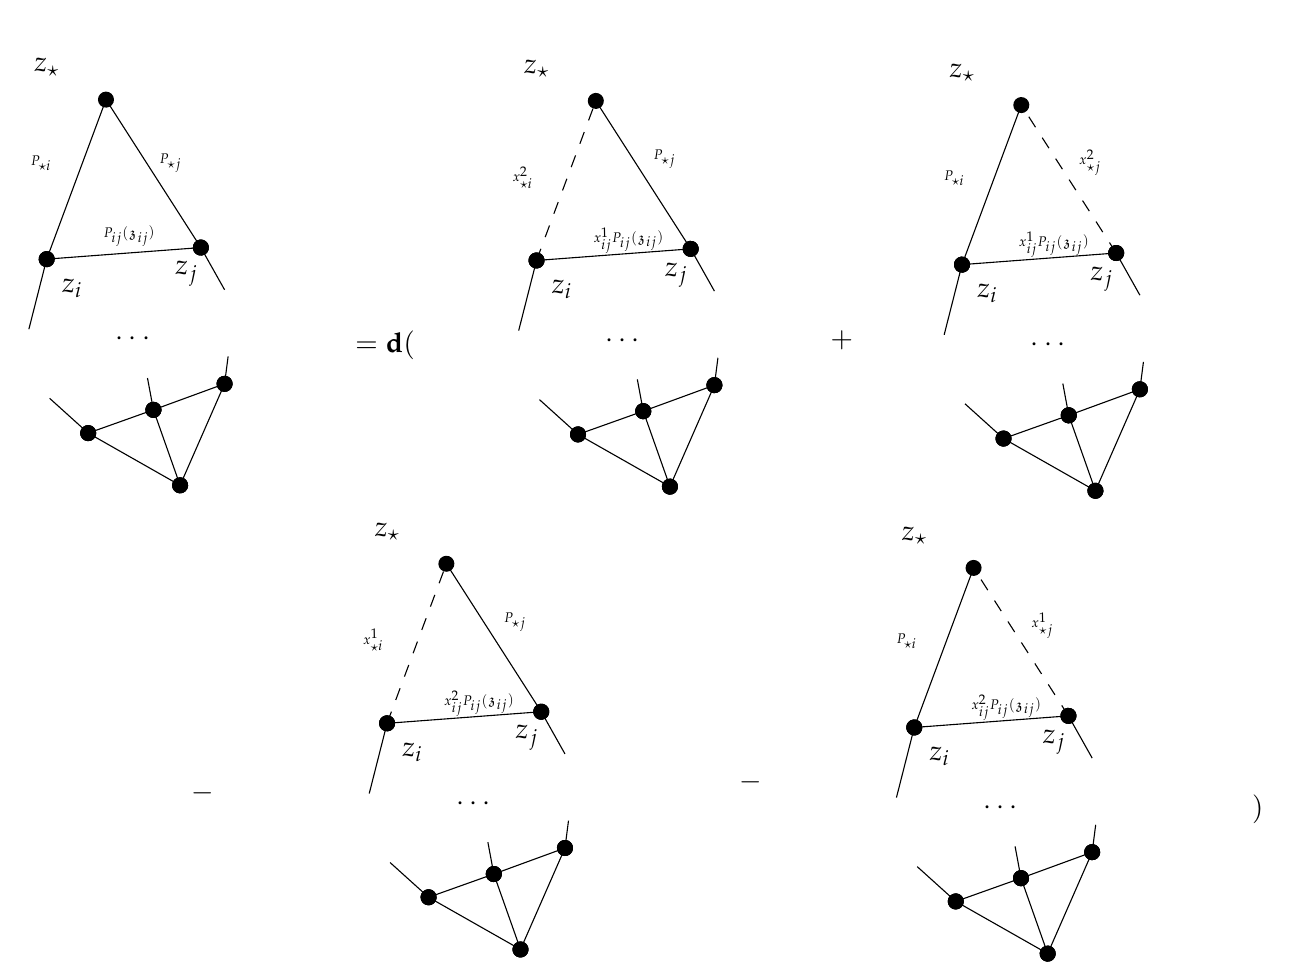
\begin{tikzpicture}[x=0.75pt,y=0.75pt,yscale=-1,xscale=1]
%uncomment if require: \path (0,468); %set diagram left start at 0, and has height of 468

%Straight Lines [id:da05577391005151622]
\draw    (45.67,112.69) -- (74.24,35.83) ;
\draw [shift={(74.24,35.83)}, rotate = 290.39] [color={rgb, 255:red, 0; green, 0; blue, 0 }  ][fill={rgb, 255:red, 0; green, 0; blue, 0 }  ][line width=0.75]      (0, 0) circle [x radius= 3.35, y radius= 3.35]   ;
\draw [shift={(45.67,112.69)}, rotate = 290.39] [color={rgb, 255:red, 0; green, 0; blue, 0 }  ][fill={rgb, 255:red, 0; green, 0; blue, 0 }  ][line width=0.75]      (0, 0) circle [x radius= 3.35, y radius= 3.35]   ;
%Straight Lines [id:da9941994376013314]
\draw    (119.95,107.11) -- (74.24,35.83) ;
\draw [shift={(119.95,107.11)}, rotate = 237.33] [color={rgb, 255:red, 0; green, 0; blue, 0 }  ][fill={rgb, 255:red, 0; green, 0; blue, 0 }  ][line width=0.75]      (0, 0) circle [x radius= 3.35, y radius= 3.35]   ;
%Straight Lines [id:da3900565594052461]
\draw    (109.95,221.66) -- (97.1,185.3) ;
\draw [shift={(97.1,185.3)}, rotate = 250.52] [color={rgb, 255:red, 0; green, 0; blue, 0 }  ][fill={rgb, 255:red, 0; green, 0; blue, 0 }  ][line width=0.75]      (0, 0) circle [x radius= 3.35, y radius= 3.35]   ;
\draw [shift={(109.95,221.66)}, rotate = 250.52] [color={rgb, 255:red, 0; green, 0; blue, 0 }  ][fill={rgb, 255:red, 0; green, 0; blue, 0 }  ][line width=0.75]      (0, 0) circle [x radius= 3.35, y radius= 3.35]   ;
%Straight Lines [id:da39495241281601645]
\draw    (119.95,107.11) -- (45.67,112.69) ;
\draw [shift={(45.67,112.69)}, rotate = 175.7] [color={rgb, 255:red, 0; green, 0; blue, 0 }  ][fill={rgb, 255:red, 0; green, 0; blue, 0 }  ][line width=0.75]      (0, 0) circle [x radius= 3.35, y radius= 3.35]   ;
\draw [shift={(119.95,107.11)}, rotate = 175.7] [color={rgb, 255:red, 0; green, 0; blue, 0 }  ][fill={rgb, 255:red, 0; green, 0; blue, 0 }  ][line width=0.75]      (0, 0) circle [x radius= 3.35, y radius= 3.35]   ;
%Straight Lines [id:da3458843670282836]
\draw    (65.67,196.51) -- (97.1,185.3) ;
\draw [shift={(97.1,185.3)}, rotate = 340.37] [color={rgb, 255:red, 0; green, 0; blue, 0 }  ][fill={rgb, 255:red, 0; green, 0; blue, 0 }  ][line width=0.75]      (0, 0) circle [x radius= 3.35, y radius= 3.35]   ;
\draw [shift={(65.67,196.51)}, rotate = 340.37] [color={rgb, 255:red, 0; green, 0; blue, 0 }  ][fill={rgb, 255:red, 0; green, 0; blue, 0 }  ][line width=0.75]      (0, 0) circle [x radius= 3.35, y radius= 3.35]   ;
%Straight Lines [id:da3629575229618873]
\draw    (65.67,196.51) -- (109.95,221.66) ;
\draw [shift={(109.95,221.66)}, rotate = 29.59] [color={rgb, 255:red, 0; green, 0; blue, 0 }  ][fill={rgb, 255:red, 0; green, 0; blue, 0 }  ][line width=0.75]      (0, 0) circle [x radius= 3.35, y radius= 3.35]   ;
\draw [shift={(65.67,196.51)}, rotate = 29.59] [color={rgb, 255:red, 0; green, 0; blue, 0 }  ][fill={rgb, 255:red, 0; green, 0; blue, 0 }  ][line width=0.75]      (0, 0) circle [x radius= 3.35, y radius= 3.35]   ;
%Straight Lines [id:da7374047900805547]
\draw    (45.67,112.69) -- (37.08,146.48) ;
\draw [shift={(45.67,112.69)}, rotate = 104.26] [color={rgb, 255:red, 0; green, 0; blue, 0 }  ][fill={rgb, 255:red, 0; green, 0; blue, 0 }  ][line width=0.75]      (0, 0) circle [x radius= 3.35, y radius= 3.35]   ;
%Straight Lines [id:da7354249192448576]
\draw    (119.95,107.11) -- (131.38,127.44) ;
\draw [shift={(119.95,107.11)}, rotate = 60.66] [color={rgb, 255:red, 0; green, 0; blue, 0 }  ][fill={rgb, 255:red, 0; green, 0; blue, 0 }  ][line width=0.75]      (0, 0) circle [x radius= 3.35, y radius= 3.35]   ;
%Straight Lines [id:da7512691918844618]
\draw    (97.1,185.3) -- (131.38,172.76) ;
\draw [shift={(131.38,172.76)}, rotate = 339.91] [color={rgb, 255:red, 0; green, 0; blue, 0 }  ][fill={rgb, 255:red, 0; green, 0; blue, 0 }  ][line width=0.75]      (0, 0) circle [x radius= 3.35, y radius= 3.35]   ;
\draw [shift={(97.1,185.3)}, rotate = 339.91] [color={rgb, 255:red, 0; green, 0; blue, 0 }  ][fill={rgb, 255:red, 0; green, 0; blue, 0 }  ][line width=0.75]      (0, 0) circle [x radius= 3.35, y radius= 3.35]   ;
%Straight Lines [id:da4433747900500091]
\draw    (65.67,196.51) -- (47.1,179.75) ;
\draw [shift={(65.67,196.51)}, rotate = 222.07] [color={rgb, 255:red, 0; green, 0; blue, 0 }  ][fill={rgb, 255:red, 0; green, 0; blue, 0 }  ][line width=0.75]      (0, 0) circle [x radius= 3.35, y radius= 3.35]   ;
%Straight Lines [id:da8725889104604558]
\draw    (97.1,185.3) -- (94.24,169.97) ;
\draw [shift={(97.1,185.3)}, rotate = 259.45] [color={rgb, 255:red, 0; green, 0; blue, 0 }  ][fill={rgb, 255:red, 0; green, 0; blue, 0 }  ][line width=0.75]      (0, 0) circle [x radius= 3.35, y radius= 3.35]   ;
%Straight Lines [id:da06318673435754363]
\draw    (131.38,172.76) -- (133.08,159.57) ;
\draw [shift={(131.38,172.76)}, rotate = 277.36] [color={rgb, 255:red, 0; green, 0; blue, 0 }  ][fill={rgb, 255:red, 0; green, 0; blue, 0 }  ][line width=0.75]      (0, 0) circle [x radius= 3.35, y radius= 3.35]   ;
%Straight Lines [id:da8635127857460636]
\draw    (109.95,221.66) -- (131.38,172.76) ;
\draw [shift={(131.38,172.76)}, rotate = 293.67] [color={rgb, 255:red, 0; green, 0; blue, 0 }  ][fill={rgb, 255:red, 0; green, 0; blue, 0 }  ][line width=0.75]      (0, 0) circle [x radius= 3.35, y radius= 3.35]   ;
\draw [shift={(109.95,221.66)}, rotate = 293.67] [color={rgb, 255:red, 0; green, 0; blue, 0 }  ][fill={rgb, 255:red, 0; green, 0; blue, 0 }  ][line width=0.75]      (0, 0) circle [x radius= 3.35, y radius= 3.35]   ;
%Straight Lines [id:da6079017959541106]
\draw  [dash pattern={on 4.5pt off 4.5pt}]  (281.67,113.33) -- (310.24,36.46) ;
\draw [shift={(310.24,36.46)}, rotate = 290.39] [color={rgb, 255:red, 0; green, 0; blue, 0 }  ][fill={rgb, 255:red, 0; green, 0; blue, 0 }  ][line width=0.75]      (0, 0) circle [x radius= 3.35, y radius= 3.35]   ;
\draw [shift={(281.67,113.33)}, rotate = 290.39] [color={rgb, 255:red, 0; green, 0; blue, 0 }  ][fill={rgb, 255:red, 0; green, 0; blue, 0 }  ][line width=0.75]      (0, 0) circle [x radius= 3.35, y radius= 3.35]   ;
%Straight Lines [id:da6262900974020484]
\draw    (355.95,107.74) -- (310.24,36.46) ;
\draw [shift={(355.95,107.74)}, rotate = 237.33] [color={rgb, 255:red, 0; green, 0; blue, 0 }  ][fill={rgb, 255:red, 0; green, 0; blue, 0 }  ][line width=0.75]      (0, 0) circle [x radius= 3.35, y radius= 3.35]   ;
%Straight Lines [id:da4207396882092873]
\draw    (345.95,222.29) -- (333.1,185.94) ;
\draw [shift={(333.1,185.94)}, rotate = 250.52] [color={rgb, 255:red, 0; green, 0; blue, 0 }  ][fill={rgb, 255:red, 0; green, 0; blue, 0 }  ][line width=0.75]      (0, 0) circle [x radius= 3.35, y radius= 3.35]   ;
\draw [shift={(345.95,222.29)}, rotate = 250.52] [color={rgb, 255:red, 0; green, 0; blue, 0 }  ][fill={rgb, 255:red, 0; green, 0; blue, 0 }  ][line width=0.75]      (0, 0) circle [x radius= 3.35, y radius= 3.35]   ;
%Straight Lines [id:da10130927807420287]
\draw    (355.95,107.74) -- (281.67,113.33) ;
\draw [shift={(281.67,113.33)}, rotate = 175.7] [color={rgb, 255:red, 0; green, 0; blue, 0 }  ][fill={rgb, 255:red, 0; green, 0; blue, 0 }  ][line width=0.75]      (0, 0) circle [x radius= 3.35, y radius= 3.35]   ;
\draw [shift={(355.95,107.74)}, rotate = 175.7] [color={rgb, 255:red, 0; green, 0; blue, 0 }  ][fill={rgb, 255:red, 0; green, 0; blue, 0 }  ][line width=0.75]      (0, 0) circle [x radius= 3.35, y radius= 3.35]   ;
%Straight Lines [id:da9973991574066416]
\draw    (301.67,197.14) -- (333.1,185.94) ;
\draw [shift={(333.1,185.94)}, rotate = 340.37] [color={rgb, 255:red, 0; green, 0; blue, 0 }  ][fill={rgb, 255:red, 0; green, 0; blue, 0 }  ][line width=0.75]      (0, 0) circle [x radius= 3.35, y radius= 3.35]   ;
\draw [shift={(301.67,197.14)}, rotate = 340.37] [color={rgb, 255:red, 0; green, 0; blue, 0 }  ][fill={rgb, 255:red, 0; green, 0; blue, 0 }  ][line width=0.75]      (0, 0) circle [x radius= 3.35, y radius= 3.35]   ;
%Straight Lines [id:da7208635053541128]
\draw    (301.67,197.14) -- (345.95,222.29) ;
\draw [shift={(345.95,222.29)}, rotate = 29.59] [color={rgb, 255:red, 0; green, 0; blue, 0 }  ][fill={rgb, 255:red, 0; green, 0; blue, 0 }  ][line width=0.75]      (0, 0) circle [x radius= 3.35, y radius= 3.35]   ;
\draw [shift={(301.67,197.14)}, rotate = 29.59] [color={rgb, 255:red, 0; green, 0; blue, 0 }  ][fill={rgb, 255:red, 0; green, 0; blue, 0 }  ][line width=0.75]      (0, 0) circle [x radius= 3.35, y radius= 3.35]   ;
%Straight Lines [id:da5476792808251072]
\draw    (281.67,113.33) -- (273.08,147.12) ;
\draw [shift={(281.67,113.33)}, rotate = 104.26] [color={rgb, 255:red, 0; green, 0; blue, 0 }  ][fill={rgb, 255:red, 0; green, 0; blue, 0 }  ][line width=0.75]      (0, 0) circle [x radius= 3.35, y radius= 3.35]   ;
%Straight Lines [id:da4842288863296871]
\draw    (355.95,107.74) -- (367.38,128.07) ;
\draw [shift={(355.95,107.74)}, rotate = 60.66] [color={rgb, 255:red, 0; green, 0; blue, 0 }  ][fill={rgb, 255:red, 0; green, 0; blue, 0 }  ][line width=0.75]      (0, 0) circle [x radius= 3.35, y radius= 3.35]   ;
%Straight Lines [id:da5181357205840986]
\draw    (333.1,185.94) -- (367.38,173.4) ;
\draw [shift={(367.38,173.4)}, rotate = 339.91] [color={rgb, 255:red, 0; green, 0; blue, 0 }  ][fill={rgb, 255:red, 0; green, 0; blue, 0 }  ][line width=0.75]      (0, 0) circle [x radius= 3.35, y radius= 3.35]   ;
\draw [shift={(333.1,185.94)}, rotate = 339.91] [color={rgb, 255:red, 0; green, 0; blue, 0 }  ][fill={rgb, 255:red, 0; green, 0; blue, 0 }  ][line width=0.75]      (0, 0) circle [x radius= 3.35, y radius= 3.35]   ;
%Straight Lines [id:da25998482008575174]
\draw    (301.67,197.14) -- (283.1,180.38) ;
\draw [shift={(301.67,197.14)}, rotate = 222.07] [color={rgb, 255:red, 0; green, 0; blue, 0 }  ][fill={rgb, 255:red, 0; green, 0; blue, 0 }  ][line width=0.75]      (0, 0) circle [x radius= 3.35, y radius= 3.35]   ;
%Straight Lines [id:da00593123197541745]
\draw    (333.1,185.94) -- (330.24,170.6) ;
\draw [shift={(333.1,185.94)}, rotate = 259.45] [color={rgb, 255:red, 0; green, 0; blue, 0 }  ][fill={rgb, 255:red, 0; green, 0; blue, 0 }  ][line width=0.75]      (0, 0) circle [x radius= 3.35, y radius= 3.35]   ;
%Straight Lines [id:da31696356189479014]
\draw    (367.38,173.4) -- (369.08,160.21) ;
\draw [shift={(367.38,173.4)}, rotate = 277.36] [color={rgb, 255:red, 0; green, 0; blue, 0 }  ][fill={rgb, 255:red, 0; green, 0; blue, 0 }  ][line width=0.75]      (0, 0) circle [x radius= 3.35, y radius= 3.35]   ;
%Straight Lines [id:da05067436226981181]
\draw    (345.95,222.29) -- (367.38,173.4) ;
\draw [shift={(367.38,173.4)}, rotate = 293.67] [color={rgb, 255:red, 0; green, 0; blue, 0 }  ][fill={rgb, 255:red, 0; green, 0; blue, 0 }  ][line width=0.75]      (0, 0) circle [x radius= 3.35, y radius= 3.35]   ;
\draw [shift={(345.95,222.29)}, rotate = 293.67] [color={rgb, 255:red, 0; green, 0; blue, 0 }  ][fill={rgb, 255:red, 0; green, 0; blue, 0 }  ][line width=0.75]      (0, 0) circle [x radius= 3.35, y radius= 3.35]   ;
%Straight Lines [id:da5379040559240473]
\draw  [dash pattern={on 4.5pt off 4.5pt}]  (209.67,336.33) -- (238.24,259.46) ;
\draw [shift={(238.24,259.46)}, rotate = 290.39] [color={rgb, 255:red, 0; green, 0; blue, 0 }  ][fill={rgb, 255:red, 0; green, 0; blue, 0 }  ][line width=0.75]      (0, 0) circle [x radius= 3.35, y radius= 3.35]   ;
\draw [shift={(209.67,336.33)}, rotate = 290.39] [color={rgb, 255:red, 0; green, 0; blue, 0 }  ][fill={rgb, 255:red, 0; green, 0; blue, 0 }  ][line width=0.75]      (0, 0) circle [x radius= 3.35, y radius= 3.35]   ;
%Straight Lines [id:da07964081672038281]
\draw    (283.95,330.74) -- (238.24,259.46) ;
\draw [shift={(283.95,330.74)}, rotate = 237.33] [color={rgb, 255:red, 0; green, 0; blue, 0 }  ][fill={rgb, 255:red, 0; green, 0; blue, 0 }  ][line width=0.75]      (0, 0) circle [x radius= 3.35, y radius= 3.35]   ;
%Straight Lines [id:da623421312454463]
\draw    (273.95,445.29) -- (261.1,408.94) ;
\draw [shift={(261.1,408.94)}, rotate = 250.52] [color={rgb, 255:red, 0; green, 0; blue, 0 }  ][fill={rgb, 255:red, 0; green, 0; blue, 0 }  ][line width=0.75]      (0, 0) circle [x radius= 3.35, y radius= 3.35]   ;
\draw [shift={(273.95,445.29)}, rotate = 250.52] [color={rgb, 255:red, 0; green, 0; blue, 0 }  ][fill={rgb, 255:red, 0; green, 0; blue, 0 }  ][line width=0.75]      (0, 0) circle [x radius= 3.35, y radius= 3.35]   ;
%Straight Lines [id:da12169856804436452]
\draw    (283.95,330.74) -- (209.67,336.33) ;
\draw [shift={(209.67,336.33)}, rotate = 175.7] [color={rgb, 255:red, 0; green, 0; blue, 0 }  ][fill={rgb, 255:red, 0; green, 0; blue, 0 }  ][line width=0.75]      (0, 0) circle [x radius= 3.35, y radius= 3.35]   ;
\draw [shift={(283.95,330.74)}, rotate = 175.7] [color={rgb, 255:red, 0; green, 0; blue, 0 }  ][fill={rgb, 255:red, 0; green, 0; blue, 0 }  ][line width=0.75]      (0, 0) circle [x radius= 3.35, y radius= 3.35]   ;
%Straight Lines [id:da9101675049165978]
\draw    (229.67,420.14) -- (261.1,408.94) ;
\draw [shift={(261.1,408.94)}, rotate = 340.37] [color={rgb, 255:red, 0; green, 0; blue, 0 }  ][fill={rgb, 255:red, 0; green, 0; blue, 0 }  ][line width=0.75]      (0, 0) circle [x radius= 3.35, y radius= 3.35]   ;
\draw [shift={(229.67,420.14)}, rotate = 340.37] [color={rgb, 255:red, 0; green, 0; blue, 0 }  ][fill={rgb, 255:red, 0; green, 0; blue, 0 }  ][line width=0.75]      (0, 0) circle [x radius= 3.35, y radius= 3.35]   ;
%Straight Lines [id:da043757079672652965]
\draw    (229.67,420.14) -- (273.95,445.29) ;
\draw [shift={(273.95,445.29)}, rotate = 29.59] [color={rgb, 255:red, 0; green, 0; blue, 0 }  ][fill={rgb, 255:red, 0; green, 0; blue, 0 }  ][line width=0.75]      (0, 0) circle [x radius= 3.35, y radius= 3.35]   ;
\draw [shift={(229.67,420.14)}, rotate = 29.59] [color={rgb, 255:red, 0; green, 0; blue, 0 }  ][fill={rgb, 255:red, 0; green, 0; blue, 0 }  ][line width=0.75]      (0, 0) circle [x radius= 3.35, y radius= 3.35]   ;
%Straight Lines [id:da3984530587665718]
\draw    (209.67,336.33) -- (201.08,370.12) ;
\draw [shift={(209.67,336.33)}, rotate = 104.26] [color={rgb, 255:red, 0; green, 0; blue, 0 }  ][fill={rgb, 255:red, 0; green, 0; blue, 0 }  ][line width=0.75]      (0, 0) circle [x radius= 3.35, y radius= 3.35]   ;
%Straight Lines [id:da3646360861208682]
\draw    (283.95,330.74) -- (295.38,351.07) ;
\draw [shift={(283.95,330.74)}, rotate = 60.66] [color={rgb, 255:red, 0; green, 0; blue, 0 }  ][fill={rgb, 255:red, 0; green, 0; blue, 0 }  ][line width=0.75]      (0, 0) circle [x radius= 3.35, y radius= 3.35]   ;
%Straight Lines [id:da004765418535702004]
\draw    (261.1,408.94) -- (295.38,396.4) ;
\draw [shift={(295.38,396.4)}, rotate = 339.91] [color={rgb, 255:red, 0; green, 0; blue, 0 }  ][fill={rgb, 255:red, 0; green, 0; blue, 0 }  ][line width=0.75]      (0, 0) circle [x radius= 3.35, y radius= 3.35]   ;
\draw [shift={(261.1,408.94)}, rotate = 339.91] [color={rgb, 255:red, 0; green, 0; blue, 0 }  ][fill={rgb, 255:red, 0; green, 0; blue, 0 }  ][line width=0.75]      (0, 0) circle [x radius= 3.35, y radius= 3.35]   ;
%Straight Lines [id:da4471076941500518]
\draw    (229.67,420.14) -- (211.1,403.38) ;
\draw [shift={(229.67,420.14)}, rotate = 222.07] [color={rgb, 255:red, 0; green, 0; blue, 0 }  ][fill={rgb, 255:red, 0; green, 0; blue, 0 }  ][line width=0.75]      (0, 0) circle [x radius= 3.35, y radius= 3.35]   ;
%Straight Lines [id:da8892260272577963]
\draw    (261.1,408.94) -- (258.24,393.6) ;
\draw [shift={(261.1,408.94)}, rotate = 259.45] [color={rgb, 255:red, 0; green, 0; blue, 0 }  ][fill={rgb, 255:red, 0; green, 0; blue, 0 }  ][line width=0.75]      (0, 0) circle [x radius= 3.35, y radius= 3.35]   ;
%Straight Lines [id:da5366908426898191]
\draw    (295.38,396.4) -- (297.08,383.21) ;
\draw [shift={(295.38,396.4)}, rotate = 277.36] [color={rgb, 255:red, 0; green, 0; blue, 0 }  ][fill={rgb, 255:red, 0; green, 0; blue, 0 }  ][line width=0.75]      (0, 0) circle [x radius= 3.35, y radius= 3.35]   ;
%Straight Lines [id:da6406878003707261]
\draw    (273.95,445.29) -- (295.38,396.4) ;
\draw [shift={(295.38,396.4)}, rotate = 293.67] [color={rgb, 255:red, 0; green, 0; blue, 0 }  ][fill={rgb, 255:red, 0; green, 0; blue, 0 }  ][line width=0.75]      (0, 0) circle [x radius= 3.35, y radius= 3.35]   ;
\draw [shift={(273.95,445.29)}, rotate = 293.67] [color={rgb, 255:red, 0; green, 0; blue, 0 }  ][fill={rgb, 255:red, 0; green, 0; blue, 0 }  ][line width=0.75]      (0, 0) circle [x radius= 3.35, y radius= 3.35]   ;
%Straight Lines [id:da02022332446143138]
\draw    (486.67,115.33) -- (515.24,38.46) ;
\draw [shift={(515.24,38.46)}, rotate = 290.39] [color={rgb, 255:red, 0; green, 0; blue, 0 }  ][fill={rgb, 255:red, 0; green, 0; blue, 0 }  ][line width=0.75]      (0, 0) circle [x radius= 3.35, y radius= 3.35]   ;
\draw [shift={(486.67,115.33)}, rotate = 290.39] [color={rgb, 255:red, 0; green, 0; blue, 0 }  ][fill={rgb, 255:red, 0; green, 0; blue, 0 }  ][line width=0.75]      (0, 0) circle [x radius= 3.35, y radius= 3.35]   ;
%Straight Lines [id:da5288571741275976]
\draw  [dash pattern={on 4.5pt off 4.5pt}]  (560.95,109.74) -- (515.24,38.46) ;
\draw [shift={(560.95,109.74)}, rotate = 237.33] [color={rgb, 255:red, 0; green, 0; blue, 0 }  ][fill={rgb, 255:red, 0; green, 0; blue, 0 }  ][line width=0.75]      (0, 0) circle [x radius= 3.35, y radius= 3.35]   ;
%Straight Lines [id:da5128746037479821]
\draw    (550.95,224.29) -- (538.1,187.94) ;
\draw [shift={(538.1,187.94)}, rotate = 250.52] [color={rgb, 255:red, 0; green, 0; blue, 0 }  ][fill={rgb, 255:red, 0; green, 0; blue, 0 }  ][line width=0.75]      (0, 0) circle [x radius= 3.35, y radius= 3.35]   ;
\draw [shift={(550.95,224.29)}, rotate = 250.52] [color={rgb, 255:red, 0; green, 0; blue, 0 }  ][fill={rgb, 255:red, 0; green, 0; blue, 0 }  ][line width=0.75]      (0, 0) circle [x radius= 3.35, y radius= 3.35]   ;
%Straight Lines [id:da6140123126224639]
\draw    (560.95,109.74) -- (486.67,115.33) ;
\draw [shift={(486.67,115.33)}, rotate = 175.7] [color={rgb, 255:red, 0; green, 0; blue, 0 }  ][fill={rgb, 255:red, 0; green, 0; blue, 0 }  ][line width=0.75]      (0, 0) circle [x radius= 3.35, y radius= 3.35]   ;
\draw [shift={(560.95,109.74)}, rotate = 175.7] [color={rgb, 255:red, 0; green, 0; blue, 0 }  ][fill={rgb, 255:red, 0; green, 0; blue, 0 }  ][line width=0.75]      (0, 0) circle [x radius= 3.35, y radius= 3.35]   ;
%Straight Lines [id:da7457563432649676]
\draw    (506.67,199.14) -- (538.1,187.94) ;
\draw [shift={(538.1,187.94)}, rotate = 340.37] [color={rgb, 255:red, 0; green, 0; blue, 0 }  ][fill={rgb, 255:red, 0; green, 0; blue, 0 }  ][line width=0.75]      (0, 0) circle [x radius= 3.35, y radius= 3.35]   ;
\draw [shift={(506.67,199.14)}, rotate = 340.37] [color={rgb, 255:red, 0; green, 0; blue, 0 }  ][fill={rgb, 255:red, 0; green, 0; blue, 0 }  ][line width=0.75]      (0, 0) circle [x radius= 3.35, y radius= 3.35]   ;
%Straight Lines [id:da537605841830689]
\draw    (506.67,199.14) -- (550.95,224.29) ;
\draw [shift={(550.95,224.29)}, rotate = 29.59] [color={rgb, 255:red, 0; green, 0; blue, 0 }  ][fill={rgb, 255:red, 0; green, 0; blue, 0 }  ][line width=0.75]      (0, 0) circle [x radius= 3.35, y radius= 3.35]   ;
\draw [shift={(506.67,199.14)}, rotate = 29.59] [color={rgb, 255:red, 0; green, 0; blue, 0 }  ][fill={rgb, 255:red, 0; green, 0; blue, 0 }  ][line width=0.75]      (0, 0) circle [x radius= 3.35, y radius= 3.35]   ;
%Straight Lines [id:da8002140501405561]
\draw    (486.67,115.33) -- (478.08,149.12) ;
\draw [shift={(486.67,115.33)}, rotate = 104.26] [color={rgb, 255:red, 0; green, 0; blue, 0 }  ][fill={rgb, 255:red, 0; green, 0; blue, 0 }  ][line width=0.75]      (0, 0) circle [x radius= 3.35, y radius= 3.35]   ;
%Straight Lines [id:da5909286524354338]
\draw    (560.95,109.74) -- (572.38,130.07) ;
\draw [shift={(560.95,109.74)}, rotate = 60.66] [color={rgb, 255:red, 0; green, 0; blue, 0 }  ][fill={rgb, 255:red, 0; green, 0; blue, 0 }  ][line width=0.75]      (0, 0) circle [x radius= 3.35, y radius= 3.35]   ;
%Straight Lines [id:da8937326368583083]
\draw    (538.1,187.94) -- (572.38,175.4) ;
\draw [shift={(572.38,175.4)}, rotate = 339.91] [color={rgb, 255:red, 0; green, 0; blue, 0 }  ][fill={rgb, 255:red, 0; green, 0; blue, 0 }  ][line width=0.75]      (0, 0) circle [x radius= 3.35, y radius= 3.35]   ;
\draw [shift={(538.1,187.94)}, rotate = 339.91] [color={rgb, 255:red, 0; green, 0; blue, 0 }  ][fill={rgb, 255:red, 0; green, 0; blue, 0 }  ][line width=0.75]      (0, 0) circle [x radius= 3.35, y radius= 3.35]   ;
%Straight Lines [id:da39486850360585657]
\draw    (506.67,199.14) -- (488.1,182.38) ;
\draw [shift={(506.67,199.14)}, rotate = 222.07] [color={rgb, 255:red, 0; green, 0; blue, 0 }  ][fill={rgb, 255:red, 0; green, 0; blue, 0 }  ][line width=0.75]      (0, 0) circle [x radius= 3.35, y radius= 3.35]   ;
%Straight Lines [id:da5723040194124529]
\draw    (538.1,187.94) -- (535.24,172.6) ;
\draw [shift={(538.1,187.94)}, rotate = 259.45] [color={rgb, 255:red, 0; green, 0; blue, 0 }  ][fill={rgb, 255:red, 0; green, 0; blue, 0 }  ][line width=0.75]      (0, 0) circle [x radius= 3.35, y radius= 3.35]   ;
%Straight Lines [id:da6617379630684848]
\draw    (572.38,175.4) -- (574.08,162.21) ;
\draw [shift={(572.38,175.4)}, rotate = 277.36] [color={rgb, 255:red, 0; green, 0; blue, 0 }  ][fill={rgb, 255:red, 0; green, 0; blue, 0 }  ][line width=0.75]      (0, 0) circle [x radius= 3.35, y radius= 3.35]   ;
%Straight Lines [id:da06155672117733357]
\draw    (550.95,224.29) -- (572.38,175.4) ;
\draw [shift={(572.38,175.4)}, rotate = 293.67] [color={rgb, 255:red, 0; green, 0; blue, 0 }  ][fill={rgb, 255:red, 0; green, 0; blue, 0 }  ][line width=0.75]      (0, 0) circle [x radius= 3.35, y radius= 3.35]   ;
\draw [shift={(550.95,224.29)}, rotate = 293.67] [color={rgb, 255:red, 0; green, 0; blue, 0 }  ][fill={rgb, 255:red, 0; green, 0; blue, 0 }  ][line width=0.75]      (0, 0) circle [x radius= 3.35, y radius= 3.35]   ;
%Straight Lines [id:da26570006292245996]
\draw    (463.67,338.33) -- (492.24,261.46) ;
\draw [shift={(492.24,261.46)}, rotate = 290.39] [color={rgb, 255:red, 0; green, 0; blue, 0 }  ][fill={rgb, 255:red, 0; green, 0; blue, 0 }  ][line width=0.75]      (0, 0) circle [x radius= 3.35, y radius= 3.35]   ;
\draw [shift={(463.67,338.33)}, rotate = 290.39] [color={rgb, 255:red, 0; green, 0; blue, 0 }  ][fill={rgb, 255:red, 0; green, 0; blue, 0 }  ][line width=0.75]      (0, 0) circle [x radius= 3.35, y radius= 3.35]   ;
%Straight Lines [id:da40306180015380066]
\draw  [dash pattern={on 4.5pt off 4.5pt}]  (537.95,332.74) -- (492.24,261.46) ;
\draw [shift={(537.95,332.74)}, rotate = 237.33] [color={rgb, 255:red, 0; green, 0; blue, 0 }  ][fill={rgb, 255:red, 0; green, 0; blue, 0 }  ][line width=0.75]      (0, 0) circle [x radius= 3.35, y radius= 3.35]   ;
%Straight Lines [id:da18554926508633796]
\draw    (527.95,447.29) -- (515.1,410.94) ;
\draw [shift={(515.1,410.94)}, rotate = 250.52] [color={rgb, 255:red, 0; green, 0; blue, 0 }  ][fill={rgb, 255:red, 0; green, 0; blue, 0 }  ][line width=0.75]      (0, 0) circle [x radius= 3.35, y radius= 3.35]   ;
\draw [shift={(527.95,447.29)}, rotate = 250.52] [color={rgb, 255:red, 0; green, 0; blue, 0 }  ][fill={rgb, 255:red, 0; green, 0; blue, 0 }  ][line width=0.75]      (0, 0) circle [x radius= 3.35, y radius= 3.35]   ;
%Straight Lines [id:da40858047037677103]
\draw    (537.95,332.74) -- (463.67,338.33) ;
\draw [shift={(463.67,338.33)}, rotate = 175.7] [color={rgb, 255:red, 0; green, 0; blue, 0 }  ][fill={rgb, 255:red, 0; green, 0; blue, 0 }  ][line width=0.75]      (0, 0) circle [x radius= 3.35, y radius= 3.35]   ;
\draw [shift={(537.95,332.74)}, rotate = 175.7] [color={rgb, 255:red, 0; green, 0; blue, 0 }  ][fill={rgb, 255:red, 0; green, 0; blue, 0 }  ][line width=0.75]      (0, 0) circle [x radius= 3.35, y radius= 3.35]   ;
%Straight Lines [id:da7743038002276321]
\draw    (483.67,422.14) -- (515.1,410.94) ;
\draw [shift={(515.1,410.94)}, rotate = 340.37] [color={rgb, 255:red, 0; green, 0; blue, 0 }  ][fill={rgb, 255:red, 0; green, 0; blue, 0 }  ][line width=0.75]      (0, 0) circle [x radius= 3.35, y radius= 3.35]   ;
\draw [shift={(483.67,422.14)}, rotate = 340.37] [color={rgb, 255:red, 0; green, 0; blue, 0 }  ][fill={rgb, 255:red, 0; green, 0; blue, 0 }  ][line width=0.75]      (0, 0) circle [x radius= 3.35, y radius= 3.35]   ;
%Straight Lines [id:da43373975235177076]
\draw    (483.67,422.14) -- (527.95,447.29) ;
\draw [shift={(527.95,447.29)}, rotate = 29.59] [color={rgb, 255:red, 0; green, 0; blue, 0 }  ][fill={rgb, 255:red, 0; green, 0; blue, 0 }  ][line width=0.75]      (0, 0) circle [x radius= 3.35, y radius= 3.35]   ;
\draw [shift={(483.67,422.14)}, rotate = 29.59] [color={rgb, 255:red, 0; green, 0; blue, 0 }  ][fill={rgb, 255:red, 0; green, 0; blue, 0 }  ][line width=0.75]      (0, 0) circle [x radius= 3.35, y radius= 3.35]   ;
%Straight Lines [id:da059421258991678716]
\draw    (463.67,338.33) -- (455.08,372.12) ;
\draw [shift={(463.67,338.33)}, rotate = 104.26] [color={rgb, 255:red, 0; green, 0; blue, 0 }  ][fill={rgb, 255:red, 0; green, 0; blue, 0 }  ][line width=0.75]      (0, 0) circle [x radius= 3.35, y radius= 3.35]   ;
%Straight Lines [id:da9003970058401041]
\draw    (537.95,332.74) -- (549.38,353.07) ;
\draw [shift={(537.95,332.74)}, rotate = 60.66] [color={rgb, 255:red, 0; green, 0; blue, 0 }  ][fill={rgb, 255:red, 0; green, 0; blue, 0 }  ][line width=0.75]      (0, 0) circle [x radius= 3.35, y radius= 3.35]   ;
%Straight Lines [id:da7049527604866348]
\draw    (515.1,410.94) -- (549.38,398.4) ;
\draw [shift={(549.38,398.4)}, rotate = 339.91] [color={rgb, 255:red, 0; green, 0; blue, 0 }  ][fill={rgb, 255:red, 0; green, 0; blue, 0 }  ][line width=0.75]      (0, 0) circle [x radius= 3.35, y radius= 3.35]   ;
\draw [shift={(515.1,410.94)}, rotate = 339.91] [color={rgb, 255:red, 0; green, 0; blue, 0 }  ][fill={rgb, 255:red, 0; green, 0; blue, 0 }  ][line width=0.75]      (0, 0) circle [x radius= 3.35, y radius= 3.35]   ;
%Straight Lines [id:da30853022450967305]
\draw    (483.67,422.14) -- (465.1,405.38) ;
\draw [shift={(483.67,422.14)}, rotate = 222.07] [color={rgb, 255:red, 0; green, 0; blue, 0 }  ][fill={rgb, 255:red, 0; green, 0; blue, 0 }  ][line width=0.75]      (0, 0) circle [x radius= 3.35, y radius= 3.35]   ;
%Straight Lines [id:da8152787882036101]
\draw    (515.1,410.94) -- (512.24,395.6) ;
\draw [shift={(515.1,410.94)}, rotate = 259.45] [color={rgb, 255:red, 0; green, 0; blue, 0 }  ][fill={rgb, 255:red, 0; green, 0; blue, 0 }  ][line width=0.75]      (0, 0) circle [x radius= 3.35, y radius= 3.35]   ;
%Straight Lines [id:da5978237424415016]
\draw    (549.38,398.4) -- (551.08,385.21) ;
\draw [shift={(549.38,398.4)}, rotate = 277.36] [color={rgb, 255:red, 0; green, 0; blue, 0 }  ][fill={rgb, 255:red, 0; green, 0; blue, 0 }  ][line width=0.75]      (0, 0) circle [x radius= 3.35, y radius= 3.35]   ;
%Straight Lines [id:da6023515255937397]
\draw    (527.95,447.29) -- (549.38,398.4) ;
\draw [shift={(549.38,398.4)}, rotate = 293.67] [color={rgb, 255:red, 0; green, 0; blue, 0 }  ][fill={rgb, 255:red, 0; green, 0; blue, 0 }  ][line width=0.75]      (0, 0) circle [x radius= 3.35, y radius= 3.35]   ;
\draw [shift={(527.95,447.29)}, rotate = 293.67] [color={rgb, 255:red, 0; green, 0; blue, 0 }  ][fill={rgb, 255:red, 0; green, 0; blue, 0 }  ][line width=0.75]      (0, 0) circle [x radius= 3.35, y radius= 3.35]   ;

% Text Node
\draw (38.19,14.77) node [anchor=north west][inner sep=0.75pt]    {$z_{\star }$};
% Text Node
\draw (106.1,112.48) node [anchor=north west][inner sep=0.75pt]    {$z_{j}{}$};
% Text Node
\draw (51.53,120.86) node [anchor=north west][inner sep=0.75pt]    {$z_{i}$};
% Text Node
\draw (77.48,147.08) node [anchor=north west][inner sep=0.75pt]    {$\cdots $};
% Text Node
\draw (71.78,95.9) node [anchor=north west][inner sep=0.75pt]  [font=\tiny,rotate=-359.06]  {$P_{ij}(\mathfrak{z}_{ij})$};
% Text Node
\draw (192.98,145.94) node [anchor=north west][inner sep=0.75pt]    {$=\mathbf{d}($};
% Text Node
\draw (274.19,15.4) node [anchor=north west][inner sep=0.75pt]    {$z_{\star }$};
% Text Node
\draw (342.1,113.11) node [anchor=north west][inner sep=0.75pt]    {$z_{j}{}$};
% Text Node
\draw (287.53,121.49) node [anchor=north west][inner sep=0.75pt]    {$z_{i}$};
% Text Node
\draw (313.48,147.71) node [anchor=north west][inner sep=0.75pt]    {$\cdots $};
% Text Node
\draw (307.78,96.54) node [anchor=north west][inner sep=0.75pt]  [font=\tiny,rotate=-359.06]  {$x_{ij}^{1} P_{ij}(\mathfrak{z}_{ij})$};
% Text Node
\draw (36.78,61.9) node [anchor=north west][inner sep=0.75pt]  [font=\tiny,rotate=-359.06]  {$P_{\star i}$};
% Text Node
\draw (98.78,60.9) node [anchor=north west][inner sep=0.75pt]  [font=\tiny,rotate=-359.06]  {$P_{\star j}$};
% Text Node
\draw (268.78,66.9) node [anchor=north west][inner sep=0.75pt]  [font=\tiny,rotate=-359.06]  {$x_{\star i}^{2}$};
% Text Node
\draw (336.78,58.9) node [anchor=north west][inner sep=0.75pt]  [font=\tiny,rotate=-359.06]  {$P_{\star j}$};
% Text Node
\draw (421.98,145.94) node [anchor=north west][inner sep=0.75pt]    {$+$};
% Text Node
\draw (202.19,238.4) node [anchor=north west][inner sep=0.75pt]    {$z_{\star }$};
% Text Node
\draw (270.1,336.11) node [anchor=north west][inner sep=0.75pt]    {$z_{j}{}$};
% Text Node
\draw (215.53,344.49) node [anchor=north west][inner sep=0.75pt]    {$z_{i}$};
% Text Node
\draw (241.48,370.71) node [anchor=north west][inner sep=0.75pt]    {$\cdots $};
% Text Node
\draw (235.78,319.54) node [anchor=north west][inner sep=0.75pt]  [font=\tiny,rotate=-359.06]  {$x_{ij}^{2} P_{ij}(\mathfrak{z}_{ij})$};
% Text Node
\draw (196.78,289.9) node [anchor=north west][inner sep=0.75pt]  [font=\tiny,rotate=-359.06]  {$x_{\star i}^{1}$};
% Text Node
\draw (264.78,281.9) node [anchor=north west][inner sep=0.75pt]  [font=\tiny,rotate=-359.06]  {$P_{\star j}$};
% Text Node
\draw (113.98,363.94) node [anchor=north west][inner sep=0.75pt]    {$-$};
% Text Node
\draw (479.19,17.4) node [anchor=north west][inner sep=0.75pt]    {$z_{\star }$};
% Text Node
\draw (547.1,115.11) node [anchor=north west][inner sep=0.75pt]    {$z_{j}{}$};
% Text Node
\draw (492.53,123.49) node [anchor=north west][inner sep=0.75pt]    {$z_{i}$};
% Text Node
\draw (518.48,149.71) node [anchor=north west][inner sep=0.75pt]    {$\cdots $};
% Text Node
\draw (512.78,98.54) node [anchor=north west][inner sep=0.75pt]  [font=\tiny,rotate=-359.06]  {$x_{ij}^{1} P_{ij}(\mathfrak{z}_{ij})$};
% Text Node
\draw (541.78,58.9) node [anchor=north west][inner sep=0.75pt]  [font=\tiny,rotate=-359.06]  {$x_{\star j}^{2}$};
% Text Node
\draw (476.78,68.9) node [anchor=north west][inner sep=0.75pt]  [font=\tiny,rotate=-359.06]  {$P_{\star i}$};
% Text Node
\draw (377.98,358.94) node [anchor=north west][inner sep=0.75pt]    {$-$};
% Text Node
\draw (456.19,240.4) node [anchor=north west][inner sep=0.75pt]    {$z_{\star }$};
% Text Node
\draw (524.1,338.11) node [anchor=north west][inner sep=0.75pt]    {$z_{j}{}$};
% Text Node
\draw (469.53,346.49) node [anchor=north west][inner sep=0.75pt]    {$z_{i}$};
% Text Node
\draw (495.48,372.71) node [anchor=north west][inner sep=0.75pt]    {$\cdots $};
% Text Node
\draw (489.78,321.54) node [anchor=north west][inner sep=0.75pt]  [font=\tiny,rotate=-359.06]  {$x_{ij}^{2} P_{ij}(\mathfrak{z}_{ij})$};
% Text Node
\draw (518.78,281.9) node [anchor=north west][inner sep=0.75pt]  [font=\tiny,rotate=-359.06]  {$x_{\star j}^{1}$};
% Text Node
\draw (453.78,291.9) node [anchor=north west][inner sep=0.75pt]  [font=\tiny,rotate=-359.06]  {$P_{\star i}$};
% Text Node
\draw (625,369.4) node [anchor=north west][inner sep=0.75pt]    {$)$};


\end{tikzpicture}
  \caption{$W_{\Gamma}(\tilde{\mathfrak{z}}_{e})\cdot P_{\star i}P_{\star j}$ is exact by the Arnold relation}\label{dExactGraph}
\end{figure}
\begin{figure}[htp]
  \centering


\tikzset{every picture/.style={line width=0.75pt}} %set default line width to 0.75pt

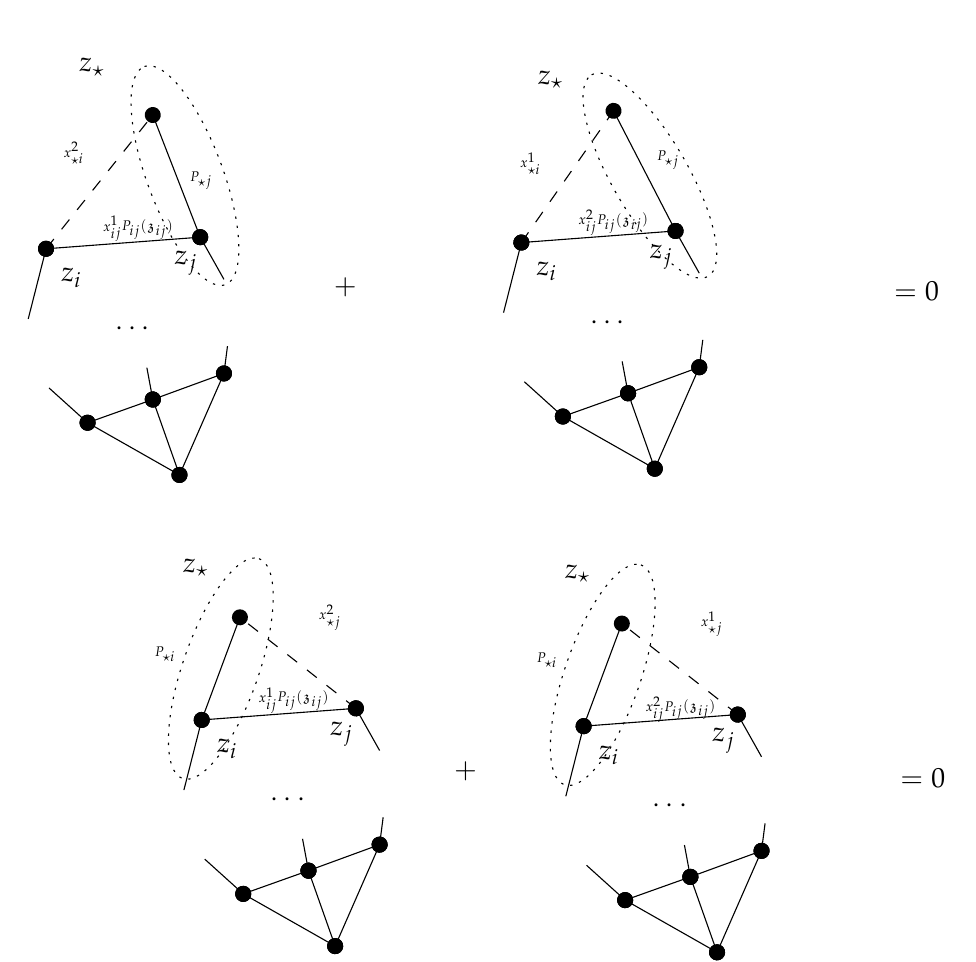
\begin{tikzpicture}[x=0.75pt,y=0.75pt,yscale=-1,xscale=1]
%uncomment if require: \path (0,499); %set diagram left start at 0, and has height of 499

%Straight Lines [id:da016701861550822983]
\draw  [dash pattern={on 4.5pt off 4.5pt}]  (49.67,112.33) -- (101.08,47.88) ;
\draw [shift={(101.08,47.88)}, rotate = 308.58] [color={rgb, 255:red, 0; green, 0; blue, 0 }  ][fill={rgb, 255:red, 0; green, 0; blue, 0 }  ][line width=0.75]      (0, 0) circle [x radius= 3.35, y radius= 3.35]   ;
\draw [shift={(49.67,112.33)}, rotate = 308.58] [color={rgb, 255:red, 0; green, 0; blue, 0 }  ][fill={rgb, 255:red, 0; green, 0; blue, 0 }  ][line width=0.75]      (0, 0) circle [x radius= 3.35, y radius= 3.35]   ;
%Straight Lines [id:da6673420184100265]
\draw    (123.95,106.74) -- (101.08,47.88) ;
\draw [shift={(123.95,106.74)}, rotate = 248.77] [color={rgb, 255:red, 0; green, 0; blue, 0 }  ][fill={rgb, 255:red, 0; green, 0; blue, 0 }  ][line width=0.75]      (0, 0) circle [x radius= 3.35, y radius= 3.35]   ;
%Straight Lines [id:da291545258927024]
\draw    (113.95,221.29) -- (101.1,184.94) ;
\draw [shift={(101.1,184.94)}, rotate = 250.52] [color={rgb, 255:red, 0; green, 0; blue, 0 }  ][fill={rgb, 255:red, 0; green, 0; blue, 0 }  ][line width=0.75]      (0, 0) circle [x radius= 3.35, y radius= 3.35]   ;
\draw [shift={(113.95,221.29)}, rotate = 250.52] [color={rgb, 255:red, 0; green, 0; blue, 0 }  ][fill={rgb, 255:red, 0; green, 0; blue, 0 }  ][line width=0.75]      (0, 0) circle [x radius= 3.35, y radius= 3.35]   ;
%Straight Lines [id:da30577453142010946]
\draw    (123.95,106.74) -- (49.67,112.33) ;
\draw [shift={(49.67,112.33)}, rotate = 175.7] [color={rgb, 255:red, 0; green, 0; blue, 0 }  ][fill={rgb, 255:red, 0; green, 0; blue, 0 }  ][line width=0.75]      (0, 0) circle [x radius= 3.35, y radius= 3.35]   ;
\draw [shift={(123.95,106.74)}, rotate = 175.7] [color={rgb, 255:red, 0; green, 0; blue, 0 }  ][fill={rgb, 255:red, 0; green, 0; blue, 0 }  ][line width=0.75]      (0, 0) circle [x radius= 3.35, y radius= 3.35]   ;
%Straight Lines [id:da3313498870535505]
\draw    (69.67,196.14) -- (101.1,184.94) ;
\draw [shift={(101.1,184.94)}, rotate = 340.37] [color={rgb, 255:red, 0; green, 0; blue, 0 }  ][fill={rgb, 255:red, 0; green, 0; blue, 0 }  ][line width=0.75]      (0, 0) circle [x radius= 3.35, y radius= 3.35]   ;
\draw [shift={(69.67,196.14)}, rotate = 340.37] [color={rgb, 255:red, 0; green, 0; blue, 0 }  ][fill={rgb, 255:red, 0; green, 0; blue, 0 }  ][line width=0.75]      (0, 0) circle [x radius= 3.35, y radius= 3.35]   ;
%Straight Lines [id:da299261848456837]
\draw    (69.67,196.14) -- (113.95,221.29) ;
\draw [shift={(113.95,221.29)}, rotate = 29.59] [color={rgb, 255:red, 0; green, 0; blue, 0 }  ][fill={rgb, 255:red, 0; green, 0; blue, 0 }  ][line width=0.75]      (0, 0) circle [x radius= 3.35, y radius= 3.35]   ;
\draw [shift={(69.67,196.14)}, rotate = 29.59] [color={rgb, 255:red, 0; green, 0; blue, 0 }  ][fill={rgb, 255:red, 0; green, 0; blue, 0 }  ][line width=0.75]      (0, 0) circle [x radius= 3.35, y radius= 3.35]   ;
%Straight Lines [id:da9810894594549351]
\draw    (49.67,112.33) -- (41.08,146.12) ;
\draw [shift={(49.67,112.33)}, rotate = 104.26] [color={rgb, 255:red, 0; green, 0; blue, 0 }  ][fill={rgb, 255:red, 0; green, 0; blue, 0 }  ][line width=0.75]      (0, 0) circle [x radius= 3.35, y radius= 3.35]   ;
%Straight Lines [id:da12287886848281349]
\draw    (123.95,106.74) -- (135.38,127.07) ;
\draw [shift={(123.95,106.74)}, rotate = 60.66] [color={rgb, 255:red, 0; green, 0; blue, 0 }  ][fill={rgb, 255:red, 0; green, 0; blue, 0 }  ][line width=0.75]      (0, 0) circle [x radius= 3.35, y radius= 3.35]   ;
%Straight Lines [id:da682096516134622]
\draw    (101.1,184.94) -- (135.38,172.4) ;
\draw [shift={(135.38,172.4)}, rotate = 339.91] [color={rgb, 255:red, 0; green, 0; blue, 0 }  ][fill={rgb, 255:red, 0; green, 0; blue, 0 }  ][line width=0.75]      (0, 0) circle [x radius= 3.35, y radius= 3.35]   ;
\draw [shift={(101.1,184.94)}, rotate = 339.91] [color={rgb, 255:red, 0; green, 0; blue, 0 }  ][fill={rgb, 255:red, 0; green, 0; blue, 0 }  ][line width=0.75]      (0, 0) circle [x radius= 3.35, y radius= 3.35]   ;
%Straight Lines [id:da6856933973629049]
\draw    (69.67,196.14) -- (51.1,179.38) ;
\draw [shift={(69.67,196.14)}, rotate = 222.07] [color={rgb, 255:red, 0; green, 0; blue, 0 }  ][fill={rgb, 255:red, 0; green, 0; blue, 0 }  ][line width=0.75]      (0, 0) circle [x radius= 3.35, y radius= 3.35]   ;
%Straight Lines [id:da2006582255893108]
\draw    (101.1,184.94) -- (98.24,169.6) ;
\draw [shift={(101.1,184.94)}, rotate = 259.45] [color={rgb, 255:red, 0; green, 0; blue, 0 }  ][fill={rgb, 255:red, 0; green, 0; blue, 0 }  ][line width=0.75]      (0, 0) circle [x radius= 3.35, y radius= 3.35]   ;
%Straight Lines [id:da6590264087471263]
\draw    (135.38,172.4) -- (137.08,159.21) ;
\draw [shift={(135.38,172.4)}, rotate = 277.36] [color={rgb, 255:red, 0; green, 0; blue, 0 }  ][fill={rgb, 255:red, 0; green, 0; blue, 0 }  ][line width=0.75]      (0, 0) circle [x radius= 3.35, y radius= 3.35]   ;
%Straight Lines [id:da34426877079033824]
\draw    (113.95,221.29) -- (135.38,172.4) ;
\draw [shift={(135.38,172.4)}, rotate = 293.67] [color={rgb, 255:red, 0; green, 0; blue, 0 }  ][fill={rgb, 255:red, 0; green, 0; blue, 0 }  ][line width=0.75]      (0, 0) circle [x radius= 3.35, y radius= 3.35]   ;
\draw [shift={(113.95,221.29)}, rotate = 293.67] [color={rgb, 255:red, 0; green, 0; blue, 0 }  ][fill={rgb, 255:red, 0; green, 0; blue, 0 }  ][line width=0.75]      (0, 0) circle [x radius= 3.35, y radius= 3.35]   ;
%Straight Lines [id:da7372440454354685]
\draw  [dash pattern={on 4.5pt off 4.5pt}]  (278.67,109.33) -- (323.08,45.88) ;
\draw [shift={(323.08,45.88)}, rotate = 304.99] [color={rgb, 255:red, 0; green, 0; blue, 0 }  ][fill={rgb, 255:red, 0; green, 0; blue, 0 }  ][line width=0.75]      (0, 0) circle [x radius= 3.35, y radius= 3.35]   ;
\draw [shift={(278.67,109.33)}, rotate = 304.99] [color={rgb, 255:red, 0; green, 0; blue, 0 }  ][fill={rgb, 255:red, 0; green, 0; blue, 0 }  ][line width=0.75]      (0, 0) circle [x radius= 3.35, y radius= 3.35]   ;
%Straight Lines [id:da2825766414379851]
\draw    (352.95,103.74) -- (323.08,45.88) ;
\draw [shift={(352.95,103.74)}, rotate = 242.69] [color={rgb, 255:red, 0; green, 0; blue, 0 }  ][fill={rgb, 255:red, 0; green, 0; blue, 0 }  ][line width=0.75]      (0, 0) circle [x radius= 3.35, y radius= 3.35]   ;
%Straight Lines [id:da40167171611659924]
\draw    (342.95,218.29) -- (330.1,181.94) ;
\draw [shift={(330.1,181.94)}, rotate = 250.52] [color={rgb, 255:red, 0; green, 0; blue, 0 }  ][fill={rgb, 255:red, 0; green, 0; blue, 0 }  ][line width=0.75]      (0, 0) circle [x radius= 3.35, y radius= 3.35]   ;
\draw [shift={(342.95,218.29)}, rotate = 250.52] [color={rgb, 255:red, 0; green, 0; blue, 0 }  ][fill={rgb, 255:red, 0; green, 0; blue, 0 }  ][line width=0.75]      (0, 0) circle [x radius= 3.35, y radius= 3.35]   ;
%Straight Lines [id:da3991150002283752]
\draw    (352.95,103.74) -- (278.67,109.33) ;
\draw [shift={(278.67,109.33)}, rotate = 175.7] [color={rgb, 255:red, 0; green, 0; blue, 0 }  ][fill={rgb, 255:red, 0; green, 0; blue, 0 }  ][line width=0.75]      (0, 0) circle [x radius= 3.35, y radius= 3.35]   ;
\draw [shift={(352.95,103.74)}, rotate = 175.7] [color={rgb, 255:red, 0; green, 0; blue, 0 }  ][fill={rgb, 255:red, 0; green, 0; blue, 0 }  ][line width=0.75]      (0, 0) circle [x radius= 3.35, y radius= 3.35]   ;
%Straight Lines [id:da4636329963381429]
\draw    (298.67,193.14) -- (330.1,181.94) ;
\draw [shift={(330.1,181.94)}, rotate = 340.37] [color={rgb, 255:red, 0; green, 0; blue, 0 }  ][fill={rgb, 255:red, 0; green, 0; blue, 0 }  ][line width=0.75]      (0, 0) circle [x radius= 3.35, y radius= 3.35]   ;
\draw [shift={(298.67,193.14)}, rotate = 340.37] [color={rgb, 255:red, 0; green, 0; blue, 0 }  ][fill={rgb, 255:red, 0; green, 0; blue, 0 }  ][line width=0.75]      (0, 0) circle [x radius= 3.35, y radius= 3.35]   ;
%Straight Lines [id:da9296126353581244]
\draw    (298.67,193.14) -- (342.95,218.29) ;
\draw [shift={(342.95,218.29)}, rotate = 29.59] [color={rgb, 255:red, 0; green, 0; blue, 0 }  ][fill={rgb, 255:red, 0; green, 0; blue, 0 }  ][line width=0.75]      (0, 0) circle [x radius= 3.35, y radius= 3.35]   ;
\draw [shift={(298.67,193.14)}, rotate = 29.59] [color={rgb, 255:red, 0; green, 0; blue, 0 }  ][fill={rgb, 255:red, 0; green, 0; blue, 0 }  ][line width=0.75]      (0, 0) circle [x radius= 3.35, y radius= 3.35]   ;
%Straight Lines [id:da8095525896445261]
\draw    (278.67,109.33) -- (270.08,143.12) ;
\draw [shift={(278.67,109.33)}, rotate = 104.26] [color={rgb, 255:red, 0; green, 0; blue, 0 }  ][fill={rgb, 255:red, 0; green, 0; blue, 0 }  ][line width=0.75]      (0, 0) circle [x radius= 3.35, y radius= 3.35]   ;
%Straight Lines [id:da8280296256933743]
\draw    (352.95,103.74) -- (364.38,124.07) ;
\draw [shift={(352.95,103.74)}, rotate = 60.66] [color={rgb, 255:red, 0; green, 0; blue, 0 }  ][fill={rgb, 255:red, 0; green, 0; blue, 0 }  ][line width=0.75]      (0, 0) circle [x radius= 3.35, y radius= 3.35]   ;
%Straight Lines [id:da21586336732017686]
\draw    (330.1,181.94) -- (364.38,169.4) ;
\draw [shift={(364.38,169.4)}, rotate = 339.91] [color={rgb, 255:red, 0; green, 0; blue, 0 }  ][fill={rgb, 255:red, 0; green, 0; blue, 0 }  ][line width=0.75]      (0, 0) circle [x radius= 3.35, y radius= 3.35]   ;
\draw [shift={(330.1,181.94)}, rotate = 339.91] [color={rgb, 255:red, 0; green, 0; blue, 0 }  ][fill={rgb, 255:red, 0; green, 0; blue, 0 }  ][line width=0.75]      (0, 0) circle [x radius= 3.35, y radius= 3.35]   ;
%Straight Lines [id:da7620376533304356]
\draw    (298.67,193.14) -- (280.1,176.38) ;
\draw [shift={(298.67,193.14)}, rotate = 222.07] [color={rgb, 255:red, 0; green, 0; blue, 0 }  ][fill={rgb, 255:red, 0; green, 0; blue, 0 }  ][line width=0.75]      (0, 0) circle [x radius= 3.35, y radius= 3.35]   ;
%Straight Lines [id:da593740390455542]
\draw    (330.1,181.94) -- (327.24,166.6) ;
\draw [shift={(330.1,181.94)}, rotate = 259.45] [color={rgb, 255:red, 0; green, 0; blue, 0 }  ][fill={rgb, 255:red, 0; green, 0; blue, 0 }  ][line width=0.75]      (0, 0) circle [x radius= 3.35, y radius= 3.35]   ;
%Straight Lines [id:da39315643175806314]
\draw    (364.38,169.4) -- (366.08,156.21) ;
\draw [shift={(364.38,169.4)}, rotate = 277.36] [color={rgb, 255:red, 0; green, 0; blue, 0 }  ][fill={rgb, 255:red, 0; green, 0; blue, 0 }  ][line width=0.75]      (0, 0) circle [x radius= 3.35, y radius= 3.35]   ;
%Straight Lines [id:da32162649978428925]
\draw    (342.95,218.29) -- (364.38,169.4) ;
\draw [shift={(364.38,169.4)}, rotate = 293.67] [color={rgb, 255:red, 0; green, 0; blue, 0 }  ][fill={rgb, 255:red, 0; green, 0; blue, 0 }  ][line width=0.75]      (0, 0) circle [x radius= 3.35, y radius= 3.35]   ;
\draw [shift={(342.95,218.29)}, rotate = 293.67] [color={rgb, 255:red, 0; green, 0; blue, 0 }  ][fill={rgb, 255:red, 0; green, 0; blue, 0 }  ][line width=0.75]      (0, 0) circle [x radius= 3.35, y radius= 3.35]   ;
%Straight Lines [id:da3032317735841781]
\draw    (124.67,339.33) -- (143.08,289.88) ;
\draw [shift={(143.08,289.88)}, rotate = 290.42] [color={rgb, 255:red, 0; green, 0; blue, 0 }  ][fill={rgb, 255:red, 0; green, 0; blue, 0 }  ][line width=0.75]      (0, 0) circle [x radius= 3.35, y radius= 3.35]   ;
\draw [shift={(124.67,339.33)}, rotate = 290.42] [color={rgb, 255:red, 0; green, 0; blue, 0 }  ][fill={rgb, 255:red, 0; green, 0; blue, 0 }  ][line width=0.75]      (0, 0) circle [x radius= 3.35, y radius= 3.35]   ;
%Straight Lines [id:da3474375340285918]
\draw  [dash pattern={on 4.5pt off 4.5pt}]  (198.95,333.74) -- (143.08,289.88) ;
\draw [shift={(198.95,333.74)}, rotate = 218.13] [color={rgb, 255:red, 0; green, 0; blue, 0 }  ][fill={rgb, 255:red, 0; green, 0; blue, 0 }  ][line width=0.75]      (0, 0) circle [x radius= 3.35, y radius= 3.35]   ;
%Straight Lines [id:da165277748890025]
\draw    (188.95,448.29) -- (176.1,411.94) ;
\draw [shift={(176.1,411.94)}, rotate = 250.52] [color={rgb, 255:red, 0; green, 0; blue, 0 }  ][fill={rgb, 255:red, 0; green, 0; blue, 0 }  ][line width=0.75]      (0, 0) circle [x radius= 3.35, y radius= 3.35]   ;
\draw [shift={(188.95,448.29)}, rotate = 250.52] [color={rgb, 255:red, 0; green, 0; blue, 0 }  ][fill={rgb, 255:red, 0; green, 0; blue, 0 }  ][line width=0.75]      (0, 0) circle [x radius= 3.35, y radius= 3.35]   ;
%Straight Lines [id:da397412668453182]
\draw    (198.95,333.74) -- (124.67,339.33) ;
\draw [shift={(124.67,339.33)}, rotate = 175.7] [color={rgb, 255:red, 0; green, 0; blue, 0 }  ][fill={rgb, 255:red, 0; green, 0; blue, 0 }  ][line width=0.75]      (0, 0) circle [x radius= 3.35, y radius= 3.35]   ;
\draw [shift={(198.95,333.74)}, rotate = 175.7] [color={rgb, 255:red, 0; green, 0; blue, 0 }  ][fill={rgb, 255:red, 0; green, 0; blue, 0 }  ][line width=0.75]      (0, 0) circle [x radius= 3.35, y radius= 3.35]   ;
%Straight Lines [id:da44938459851536394]
\draw    (144.67,423.14) -- (176.1,411.94) ;
\draw [shift={(176.1,411.94)}, rotate = 340.37] [color={rgb, 255:red, 0; green, 0; blue, 0 }  ][fill={rgb, 255:red, 0; green, 0; blue, 0 }  ][line width=0.75]      (0, 0) circle [x radius= 3.35, y radius= 3.35]   ;
\draw [shift={(144.67,423.14)}, rotate = 340.37] [color={rgb, 255:red, 0; green, 0; blue, 0 }  ][fill={rgb, 255:red, 0; green, 0; blue, 0 }  ][line width=0.75]      (0, 0) circle [x radius= 3.35, y radius= 3.35]   ;
%Straight Lines [id:da3704675773059698]
\draw    (144.67,423.14) -- (188.95,448.29) ;
\draw [shift={(188.95,448.29)}, rotate = 29.59] [color={rgb, 255:red, 0; green, 0; blue, 0 }  ][fill={rgb, 255:red, 0; green, 0; blue, 0 }  ][line width=0.75]      (0, 0) circle [x radius= 3.35, y radius= 3.35]   ;
\draw [shift={(144.67,423.14)}, rotate = 29.59] [color={rgb, 255:red, 0; green, 0; blue, 0 }  ][fill={rgb, 255:red, 0; green, 0; blue, 0 }  ][line width=0.75]      (0, 0) circle [x radius= 3.35, y radius= 3.35]   ;
%Straight Lines [id:da48205725415781386]
\draw    (124.67,339.33) -- (116.08,373.12) ;
\draw [shift={(124.67,339.33)}, rotate = 104.26] [color={rgb, 255:red, 0; green, 0; blue, 0 }  ][fill={rgb, 255:red, 0; green, 0; blue, 0 }  ][line width=0.75]      (0, 0) circle [x radius= 3.35, y radius= 3.35]   ;
%Straight Lines [id:da9315082783753994]
\draw    (198.95,333.74) -- (210.38,354.07) ;
\draw [shift={(198.95,333.74)}, rotate = 60.66] [color={rgb, 255:red, 0; green, 0; blue, 0 }  ][fill={rgb, 255:red, 0; green, 0; blue, 0 }  ][line width=0.75]      (0, 0) circle [x radius= 3.35, y radius= 3.35]   ;
%Straight Lines [id:da362339232985051]
\draw    (176.1,411.94) -- (210.38,399.4) ;
\draw [shift={(210.38,399.4)}, rotate = 339.91] [color={rgb, 255:red, 0; green, 0; blue, 0 }  ][fill={rgb, 255:red, 0; green, 0; blue, 0 }  ][line width=0.75]      (0, 0) circle [x radius= 3.35, y radius= 3.35]   ;
\draw [shift={(176.1,411.94)}, rotate = 339.91] [color={rgb, 255:red, 0; green, 0; blue, 0 }  ][fill={rgb, 255:red, 0; green, 0; blue, 0 }  ][line width=0.75]      (0, 0) circle [x radius= 3.35, y radius= 3.35]   ;
%Straight Lines [id:da6388701280697504]
\draw    (144.67,423.14) -- (126.1,406.38) ;
\draw [shift={(144.67,423.14)}, rotate = 222.07] [color={rgb, 255:red, 0; green, 0; blue, 0 }  ][fill={rgb, 255:red, 0; green, 0; blue, 0 }  ][line width=0.75]      (0, 0) circle [x radius= 3.35, y radius= 3.35]   ;
%Straight Lines [id:da4393981169899286]
\draw    (176.1,411.94) -- (173.24,396.6) ;
\draw [shift={(176.1,411.94)}, rotate = 259.45] [color={rgb, 255:red, 0; green, 0; blue, 0 }  ][fill={rgb, 255:red, 0; green, 0; blue, 0 }  ][line width=0.75]      (0, 0) circle [x radius= 3.35, y radius= 3.35]   ;
%Straight Lines [id:da7727675541044259]
\draw    (210.38,399.4) -- (212.08,386.21) ;
\draw [shift={(210.38,399.4)}, rotate = 277.36] [color={rgb, 255:red, 0; green, 0; blue, 0 }  ][fill={rgb, 255:red, 0; green, 0; blue, 0 }  ][line width=0.75]      (0, 0) circle [x radius= 3.35, y radius= 3.35]   ;
%Straight Lines [id:da8732431429179641]
\draw    (188.95,448.29) -- (210.38,399.4) ;
\draw [shift={(210.38,399.4)}, rotate = 293.67] [color={rgb, 255:red, 0; green, 0; blue, 0 }  ][fill={rgb, 255:red, 0; green, 0; blue, 0 }  ][line width=0.75]      (0, 0) circle [x radius= 3.35, y radius= 3.35]   ;
\draw [shift={(188.95,448.29)}, rotate = 293.67] [color={rgb, 255:red, 0; green, 0; blue, 0 }  ][fill={rgb, 255:red, 0; green, 0; blue, 0 }  ][line width=0.75]      (0, 0) circle [x radius= 3.35, y radius= 3.35]   ;
%Shape: Ellipse [id:dp054723026974621725]
\draw  [dash pattern={on 0.84pt off 2.51pt}] (312.54,28.49) .. controls (321.28,23.44) and (340.93,41.1) .. (356.41,67.93) .. controls (371.9,94.76) and (377.37,120.6) .. (368.63,125.65) .. controls (359.89,130.69) and (340.24,113.04) .. (324.75,86.21) .. controls (309.26,59.38) and (303.8,33.54) .. (312.54,28.49) -- cycle ;
%Shape: Ellipse [id:dp5426866590205677]
\draw  [dash pattern={on 0.84pt off 2.51pt}] (97.07,24.48) .. controls (106.53,20.97) and (122.94,41.67) .. (133.72,70.71) .. controls (144.5,99.75) and (145.56,126.15) .. (136.1,129.66) .. controls (126.64,133.17) and (110.23,112.47) .. (99.45,83.43) .. controls (88.67,54.39) and (87.6,27.99) .. (97.07,24.48) -- cycle ;
%Shape: Ellipse [id:dp8432340335804664]
\draw  [dash pattern={on 0.84pt off 2.51pt}] (152.29,261.62) .. controls (161.82,264.93) and (161.31,291.34) .. (151.14,320.61) .. controls (140.98,349.87) and (125,370.9) .. (115.47,367.59) .. controls (105.93,364.28) and (106.44,337.87) .. (116.61,308.61) .. controls (126.78,279.34) and (142.75,258.31) .. (152.29,261.62) -- cycle ;
%Straight Lines [id:da1625791202902105]
\draw    (308.67,342.33) -- (327.08,292.88) ;
\draw [shift={(327.08,292.88)}, rotate = 290.42] [color={rgb, 255:red, 0; green, 0; blue, 0 }  ][fill={rgb, 255:red, 0; green, 0; blue, 0 }  ][line width=0.75]      (0, 0) circle [x radius= 3.35, y radius= 3.35]   ;
\draw [shift={(308.67,342.33)}, rotate = 290.42] [color={rgb, 255:red, 0; green, 0; blue, 0 }  ][fill={rgb, 255:red, 0; green, 0; blue, 0 }  ][line width=0.75]      (0, 0) circle [x radius= 3.35, y radius= 3.35]   ;
%Straight Lines [id:da746432742696095]
\draw  [dash pattern={on 4.5pt off 4.5pt}]  (382.95,336.74) -- (327.08,292.88) ;
\draw [shift={(382.95,336.74)}, rotate = 218.13] [color={rgb, 255:red, 0; green, 0; blue, 0 }  ][fill={rgb, 255:red, 0; green, 0; blue, 0 }  ][line width=0.75]      (0, 0) circle [x radius= 3.35, y radius= 3.35]   ;
%Straight Lines [id:da17219373332834387]
\draw    (372.95,451.29) -- (360.1,414.94) ;
\draw [shift={(360.1,414.94)}, rotate = 250.52] [color={rgb, 255:red, 0; green, 0; blue, 0 }  ][fill={rgb, 255:red, 0; green, 0; blue, 0 }  ][line width=0.75]      (0, 0) circle [x radius= 3.35, y radius= 3.35]   ;
\draw [shift={(372.95,451.29)}, rotate = 250.52] [color={rgb, 255:red, 0; green, 0; blue, 0 }  ][fill={rgb, 255:red, 0; green, 0; blue, 0 }  ][line width=0.75]      (0, 0) circle [x radius= 3.35, y radius= 3.35]   ;
%Straight Lines [id:da4621347064619983]
\draw    (382.95,336.74) -- (308.67,342.33) ;
\draw [shift={(308.67,342.33)}, rotate = 175.7] [color={rgb, 255:red, 0; green, 0; blue, 0 }  ][fill={rgb, 255:red, 0; green, 0; blue, 0 }  ][line width=0.75]      (0, 0) circle [x radius= 3.35, y radius= 3.35]   ;
\draw [shift={(382.95,336.74)}, rotate = 175.7] [color={rgb, 255:red, 0; green, 0; blue, 0 }  ][fill={rgb, 255:red, 0; green, 0; blue, 0 }  ][line width=0.75]      (0, 0) circle [x radius= 3.35, y radius= 3.35]   ;
%Straight Lines [id:da23173002946728105]
\draw    (328.67,426.14) -- (360.1,414.94) ;
\draw [shift={(360.1,414.94)}, rotate = 340.37] [color={rgb, 255:red, 0; green, 0; blue, 0 }  ][fill={rgb, 255:red, 0; green, 0; blue, 0 }  ][line width=0.75]      (0, 0) circle [x radius= 3.35, y radius= 3.35]   ;
\draw [shift={(328.67,426.14)}, rotate = 340.37] [color={rgb, 255:red, 0; green, 0; blue, 0 }  ][fill={rgb, 255:red, 0; green, 0; blue, 0 }  ][line width=0.75]      (0, 0) circle [x radius= 3.35, y radius= 3.35]   ;
%Straight Lines [id:da5632624463997629]
\draw    (328.67,426.14) -- (372.95,451.29) ;
\draw [shift={(372.95,451.29)}, rotate = 29.59] [color={rgb, 255:red, 0; green, 0; blue, 0 }  ][fill={rgb, 255:red, 0; green, 0; blue, 0 }  ][line width=0.75]      (0, 0) circle [x radius= 3.35, y radius= 3.35]   ;
\draw [shift={(328.67,426.14)}, rotate = 29.59] [color={rgb, 255:red, 0; green, 0; blue, 0 }  ][fill={rgb, 255:red, 0; green, 0; blue, 0 }  ][line width=0.75]      (0, 0) circle [x radius= 3.35, y radius= 3.35]   ;
%Straight Lines [id:da6318864871870671]
\draw    (308.67,342.33) -- (300.08,376.12) ;
\draw [shift={(308.67,342.33)}, rotate = 104.26] [color={rgb, 255:red, 0; green, 0; blue, 0 }  ][fill={rgb, 255:red, 0; green, 0; blue, 0 }  ][line width=0.75]      (0, 0) circle [x radius= 3.35, y radius= 3.35]   ;
%Straight Lines [id:da17370773737391154]
\draw    (382.95,336.74) -- (394.38,357.07) ;
\draw [shift={(382.95,336.74)}, rotate = 60.66] [color={rgb, 255:red, 0; green, 0; blue, 0 }  ][fill={rgb, 255:red, 0; green, 0; blue, 0 }  ][line width=0.75]      (0, 0) circle [x radius= 3.35, y radius= 3.35]   ;
%Straight Lines [id:da9219816290172171]
\draw    (360.1,414.94) -- (394.38,402.4) ;
\draw [shift={(394.38,402.4)}, rotate = 339.91] [color={rgb, 255:red, 0; green, 0; blue, 0 }  ][fill={rgb, 255:red, 0; green, 0; blue, 0 }  ][line width=0.75]      (0, 0) circle [x radius= 3.35, y radius= 3.35]   ;
\draw [shift={(360.1,414.94)}, rotate = 339.91] [color={rgb, 255:red, 0; green, 0; blue, 0 }  ][fill={rgb, 255:red, 0; green, 0; blue, 0 }  ][line width=0.75]      (0, 0) circle [x radius= 3.35, y radius= 3.35]   ;
%Straight Lines [id:da4744650663960672]
\draw    (328.67,426.14) -- (310.1,409.38) ;
\draw [shift={(328.67,426.14)}, rotate = 222.07] [color={rgb, 255:red, 0; green, 0; blue, 0 }  ][fill={rgb, 255:red, 0; green, 0; blue, 0 }  ][line width=0.75]      (0, 0) circle [x radius= 3.35, y radius= 3.35]   ;
%Straight Lines [id:da023175902953707084]
\draw    (360.1,414.94) -- (357.24,399.6) ;
\draw [shift={(360.1,414.94)}, rotate = 259.45] [color={rgb, 255:red, 0; green, 0; blue, 0 }  ][fill={rgb, 255:red, 0; green, 0; blue, 0 }  ][line width=0.75]      (0, 0) circle [x radius= 3.35, y radius= 3.35]   ;
%Straight Lines [id:da6229829657306729]
\draw    (394.38,402.4) -- (396.08,389.21) ;
\draw [shift={(394.38,402.4)}, rotate = 277.36] [color={rgb, 255:red, 0; green, 0; blue, 0 }  ][fill={rgb, 255:red, 0; green, 0; blue, 0 }  ][line width=0.75]      (0, 0) circle [x radius= 3.35, y radius= 3.35]   ;
%Straight Lines [id:da23553498408248252]
\draw    (372.95,451.29) -- (394.38,402.4) ;
\draw [shift={(394.38,402.4)}, rotate = 293.67] [color={rgb, 255:red, 0; green, 0; blue, 0 }  ][fill={rgb, 255:red, 0; green, 0; blue, 0 }  ][line width=0.75]      (0, 0) circle [x radius= 3.35, y radius= 3.35]   ;
\draw [shift={(372.95,451.29)}, rotate = 293.67] [color={rgb, 255:red, 0; green, 0; blue, 0 }  ][fill={rgb, 255:red, 0; green, 0; blue, 0 }  ][line width=0.75]      (0, 0) circle [x radius= 3.35, y radius= 3.35]   ;
%Shape: Ellipse [id:dp9089413040928458]
\draw  [dash pattern={on 0.84pt off 2.51pt}] (336.29,264.62) .. controls (345.82,267.93) and (345.31,294.34) .. (335.14,323.61) .. controls (324.98,352.87) and (309,373.9) .. (299.47,370.59) .. controls (289.93,367.28) and (290.44,340.87) .. (300.61,311.61) .. controls (310.78,282.34) and (326.75,261.31) .. (336.29,264.62) -- cycle ;

% Text Node
\draw (456.98,126.94) node [anchor=north west][inner sep=0.75pt]    {$=0$};
% Text Node
\draw (64.19,19.4) node [anchor=north west][inner sep=0.75pt]    {$z_{\star }$};
% Text Node
\draw (110.1,112.11) node [anchor=north west][inner sep=0.75pt]    {$z_{j}{}$};
% Text Node
\draw (55.53,120.49) node [anchor=north west][inner sep=0.75pt]    {$z_{i}$};
% Text Node
\draw (81.48,146.71) node [anchor=north west][inner sep=0.75pt]    {$\cdots $};
% Text Node
\draw (75.78,95.54) node [anchor=north west][inner sep=0.75pt]  [font=\tiny,rotate=-359.06]  {$x_{ij}^{1} P_{ij}(\mathfrak{z}_{ij})$};
% Text Node
\draw (56.78,59.9) node [anchor=north west][inner sep=0.75pt]  [font=\tiny,rotate=-359.06]  {$x_{\star i}^{2}$};
% Text Node
\draw (117.78,73.9) node [anchor=north west][inner sep=0.75pt]  [font=\tiny,rotate=-359.06]  {$P_{\star j}$};
% Text Node
\draw (186.98,124.94) node [anchor=north west][inner sep=0.75pt]    {$+$};
% Text Node
\draw (285.19,25.4) node [anchor=north west][inner sep=0.75pt]    {$z_{\star }$};
% Text Node
\draw (339.1,109.11) node [anchor=north west][inner sep=0.75pt]    {$z_{j}{}$};
% Text Node
\draw (284.53,117.49) node [anchor=north west][inner sep=0.75pt]    {$z_{i}$};
% Text Node
\draw (310.48,143.71) node [anchor=north west][inner sep=0.75pt]    {$\cdots $};
% Text Node
\draw (304.78,92.54) node [anchor=north west][inner sep=0.75pt]  [font=\tiny,rotate=-359.06]  {$x_{ij}^{2} P_{ij}(\mathfrak{z}_{ij})$};
% Text Node
\draw (276.78,64.9) node [anchor=north west][inner sep=0.75pt]  [font=\tiny,rotate=-359.06]  {$x_{\star i}^{1}$};
% Text Node
\draw (342.78,63.9) node [anchor=north west][inner sep=0.75pt]  [font=\tiny,rotate=-359.06]  {$P_{\star j}$};
% Text Node
\draw (114.19,260.4) node [anchor=north west][inner sep=0.75pt]    {$z_{\star }$};
% Text Node
\draw (185.1,339.11) node [anchor=north west][inner sep=0.75pt]    {$z_{j}{}$};
% Text Node
\draw (130.53,347.49) node [anchor=north west][inner sep=0.75pt]    {$z_{i}$};
% Text Node
\draw (156.48,373.71) node [anchor=north west][inner sep=0.75pt]    {$\cdots $};
% Text Node
\draw (150.78,322.54) node [anchor=north west][inner sep=0.75pt]  [font=\tiny,rotate=-359.06]  {$x_{ij}^{1} P_{ij}(\mathfrak{z}_{ij})$};
% Text Node
\draw (179.78,282.9) node [anchor=north west][inner sep=0.75pt]  [font=\tiny,rotate=-359.06]  {$x_{\star j}^{2}$};
% Text Node
\draw (100.78,302.9) node [anchor=north west][inner sep=0.75pt]  [font=\tiny,rotate=-359.06]  {$P_{\star i}$};
% Text Node
\draw (244.98,357.94) node [anchor=north west][inner sep=0.75pt]    {$+$};
% Text Node
\draw (460,361.4) node [anchor=north west][inner sep=0.75pt]    {$=0$};
% Text Node
\draw (298.19,263.4) node [anchor=north west][inner sep=0.75pt]    {$z_{\star }$};
% Text Node
\draw (369.1,342.11) node [anchor=north west][inner sep=0.75pt]    {$z_{j}{}$};
% Text Node
\draw (314.53,350.49) node [anchor=north west][inner sep=0.75pt]    {$z_{i}$};
% Text Node
\draw (340.48,376.71) node [anchor=north west][inner sep=0.75pt]    {$\cdots $};
% Text Node
\draw (337.2,326.97) node [anchor=north west][inner sep=0.75pt]  [font=\tiny,rotate=-359.06]  {$x_{ij}^{2} P_{ij}(\mathfrak{z}_{ij})$};
% Text Node
\draw (363.78,285.9) node [anchor=north west][inner sep=0.75pt]  [font=\tiny,rotate=-359.06]  {$x_{\star j}^{1}$};
% Text Node
\draw (284.78,305.9) node [anchor=north west][inner sep=0.75pt]  [font=\tiny,rotate=-359.06]  {$P_{\star i}$};


\end{tikzpicture}
  \caption{Some cancellations}\label{Cancellations}
\end{figure}
We will only prove the formula in the case when $\star$ is joint with $i,j\in V(\Gamma)-\{o\}$ as the proof for the other case is similar. We first notice that

\begin{align*}
\mu_{\{o,1,\dots ,n,\star\}}\left(W_{\Gamma^{\star}}(\mathfrak{z}_{e})\right)   &=\mu_{\{o,1,\dots, n,\star\}}\left(W_{\Gamma}(\mathfrak{z}_{e})\cdot P_{\star i}(\mathfrak{z}_{\star i})P_{\star j}(\mathfrak{z}_{\star j})\right)     \\
   & =\mu_{\{o,1,\dots, n,\star\}}\left(W_{\Gamma}(\tilde{\mathfrak{z}}_{e})\cdot P_{\star i}P_{\star j}\right)\cdot e^{(\lambda_i|\mathfrak{z}_{i\star})+(\lambda_j|\mathfrak{z}_{j\star})}
\end{align*}
here
$$
\begin{cases}
\tilde{\mathfrak{z}}_e=\mathfrak{z}_e+\mathfrak{z}_{\star i}  , & \mbox{if } i\in V(e),e\neq ij, \\
\tilde{\mathfrak{z}}_e=\mathfrak{z}_e+\mathfrak{z}_{\star j}  , & \mbox{if } j\in V(e),e\neq ij,\\
\tilde{\mathfrak{z}}_e=\mathfrak{z}_e-\mathfrak{z}_{\star i}-\mathfrak{z}_{\star j}   , &  \mbox{if} \ e=ij,\\
\tilde{\mathfrak{z}}_e=\mathfrak{z}_e  , & \mbox{otherwise}.
\end{cases}
$$
Using Lemma \ref{RecursiveLemma}, we have
$$
  P_{\star i}P_{\star j}P_{ij}(\tilde{\mathfrak{z}}_{ij})=\mathbf{d}\left(P_{ij}(\tilde{\mathfrak{z}}_{ij})P_{\star j}\cdot x_{\star i}\wedge x_{ij}+P_{ij}(\tilde{\mathfrak{z}}_{ij})P_{\star i}\cdot x_{\star j}\wedge x_{ij}\right)
$$
Substituting this into $\mu_{\{o,1,\dots, n,\star\}}\left(W_{\Gamma}(\tilde{\mathfrak{z}}_{e})\cdot P_{\star i}P_{\star j}\right)$, we obtain (see Fig. \ref{dExactGraph} and Fig. \ref{Cancellations})
\begin{align*}
& \mu_{\{o,1,\dots, n,\star\}}\left(W_{\Gamma}(\tilde{\mathfrak{z}}_{e})\cdot P_{\star i}P_{\star j}\right)\\
  &= \mu_{\{o,1,\dots, n,\star\}}\left(\mathbf{d}\left(W_{\Gamma}(\tilde{\mathfrak{z}}_{e})P_{\star j}\cdot x_{\star i}\wedge x_{ij}+W_{\Gamma}(\tilde{\mathfrak{z}}_{e})P_{\star i}\cdot x_{\star j}\wedge x_{ij}\right)\right)  \\
   &= \mu_{\{\star,\bullet\}}\circ \mu_{\{o,1,\dots, n\}}\left(W_{\Gamma}(\tilde{\mathfrak{z}}_{e})\cdot (x_{ij}\wedge x_{\star j})P_{\star i }\right)+\mu_{\{\star,\bullet\}}\circ \mu_{\{1\dots n\}}\left(W_{\Gamma}(\tilde{\mathfrak{z}}_{e})\cdot (x_{ij}\wedge x_{\star i})P_{\star j}\right)\\
   &+ \underbrace{ \mu_{\{o,1,\dots ,n\}}\circ\mu_{\{\star, i\}}\left(W_{\Gamma}(\tilde{\mathfrak{z}}_{e})\cdot (x_{ij}\wedge x_{\star j})P_{\star i }\right)}_{=0}+\underbrace{\mu_{\{o,1,\dots ,n\}}\circ\mu_{\{\star, j\}}\left(W_{\Gamma}(\tilde{\mathfrak{z}}_{e})\cdot (x_{ij}\wedge x_{\star i})P_{\star j}\right)}_{=0}.
\end{align*}
We will prove a stronger statement by induction. In fact, we will prove that
$$
 \sum_{\vec{e},v\in \vec{e}} \partial_{\mathfrak{z}_{\vec{e}}}  \mathbf{W}^{r,s}_{\Gamma,\mathbf{H}_{\Gamma}(o,e)}=-\lambda_v.
$$
Assume the above is true for $\mathbf{H}_{\Gamma}(o,e)$, we have
\begin{align*}
   &  \mathbf{W}^{r,s}_{\Gamma,\mathbf{H}_{\Gamma}(o,e)}(\lambda;\dots,r_{\star}\tilde{\mathfrak{z}}_{ij},\dots)\\
   & =\mathbf{W}^{r,s}_{\Gamma,\mathbf{H}_{\Gamma}(o,e)}(\lambda;\tilde{\mathfrak{z}}_{\vec{e}})-(1-r_{\star})\left(\partial_{\mathfrak{z}_{ij}}\mathbf{W}^{r,s}_{\Gamma,\mathbf{H}(o,e)}(\lambda;{\mathfrak{z}}_{\vec{e}})|\tilde{\mathfrak{z}}_{ij}\right)\\
   &=\mathbf{W}^{r,s}_{\Gamma,\mathbf{H}_{\Gamma}(o,e)}+\left(\sum_{\vec{e},i\in \vec{e}} \partial_{\mathfrak{z}_{\vec{e}}}  \mathbf{W}^{r,s}_{\Gamma,\mathbf{H}_{\Gamma}(o,e)}|\mathfrak{z}_{\star i}\right)+\left(\sum_{\vec{e},j\in \vec{e}} \partial_{\mathfrak{z}_{\vec{e}}}  \mathbf{W}^{r,s}_{\Gamma,\mathbf{H}_{\Gamma}(o,e)}|\mathfrak{z}_{\star j}\right)+(1-r_{\star})\left(\partial_{\mathfrak{z}_{ij}}\mathbf{W}^{r,s}_{\Gamma,\mathbf{H}_{\Gamma}(o,e)}|\mathfrak{z}_{\star j}-\mathfrak{z}_{\star i}-\mathfrak{z}_{ij}\right)\\
   &=\mathbf{W}^{r,s}_{\Gamma,\mathbf{H}_{\Gamma}(o,e)}-\left(\lambda_i|\mathfrak{z}_{\star i}\right)-\left(\lambda_j|\mathfrak{z}_{\star j}\right)+(1-r_{\star})\left(\partial_{\mathfrak{z}_{ij}}\mathbf{W}^{r,s}_{\Gamma,\mathbf{H}_{\Gamma}(o,e)}|\mathfrak{z}_{\star j}-\mathfrak{z}_{\star i}-\mathfrak{z}_{ij}\right)\\
   &=\mathbf{W}^{r,s}_{\Gamma,\mathbf{H}_{\Gamma}(o,e)}(\lambda;\mathfrak{z}^\triangleright_{\vec{e}})-\left(\lambda_i|\mathfrak{z}_{\star i}\right)-\left(\lambda_j|\mathfrak{z}_{\star j}\right).
\end{align*}
For simplicity of notation, we write $ \int_{\Box_{\mathbf{H}_{\Gamma}(o,e)}} $ instead of $\int_{([0,1]\times[0,1])^{|\mathbf{H}_{\Gamma}(o,e)|}} \bigwedge_{k=1,\dots,|\mathbf{H}_{\Gamma}(o,e)|} (dr_k\wedge ds_k)$. By Lemma \ref{IntegralR}, we have (for $l=1,2$)
      \begin{align*}
     &   \mu_{\{o,1,\dots, n\}}\left(W_{\Gamma}(\tilde{\mathfrak{z}}_{e})\cdot x^s_{ij}\right)\\
     &= -{\partial_{ \tilde{\mathfrak{z}}^l_{ij}}}\int^1_0\int_{\Box_{\mathbf{H}_{\Gamma}(o,e)}}  e^{   \mathbf{W}^{r,s}_{\Gamma,\mathbf{H}(o,e)}(\lambda;\dots,r_{\star}\tilde{\mathfrak{z}}_{ij},\dots)} \cdot \mathbf{G}^{r,s}_{\Gamma,\mathbf{H}_{\Gamma}(o,e)}\cdot dr_{\star}\\
     &= -\int^1_0\int_{\Box_{\mathbf{H}_{\Gamma}(o,e)}}  e^{   \mathbf{W}^{r,s}_{\Gamma,\mathbf{H}(o,e)}(\lambda;\dots,r_{\star}\tilde{\mathfrak{z}}_{ij},\dots)} {\partial_{ {\mathfrak{z}}^l_{ij}}}\mathbf{W}^{r,s}_{\Gamma,\mathbf{H}(o,e)}\cdot \mathbf{G}^{r,s}_{\Gamma,\mathbf{H}_{\Gamma}(o,e)}\cdot r_{\star}dr_{\star}\\
     &= -\int^1_0\int_{\Box_{\mathbf{H}_{\Gamma}(o,e)}}  e^{\mathbf{W}^{r,s}_{\Gamma,\mathbf{H}(o,e)}(\lambda;\mathfrak{z}_{\vec{e}}^\triangleright)-\left(\lambda_i|\mathfrak{z}_{\star i}\right)-\left(\lambda_j|\mathfrak{z}_{\star j}\right)}\cdot\mathbf{G}^{r,s}_{\Gamma,\mathbf{H}_{\Gamma}(o,e)}\cdot \partial_{\mathfrak{z}^l_{ij}}\mathbf{W}^{r,s}_{\Gamma,\mathbf{H}_{\Gamma}(o,e)}\cdot r_{\star}dr_{\star}.
     \end{align*}
    Now we Lemma \ref{IntegralS} to get
    \begin{align*}
     &   \mu_{\{\star,\bullet\}}\circ \mu_{\{o,1,\dots, n\}}\left(W_{\Gamma}(\tilde{\mathfrak{z}}_{e})\cdot (x_{ij}\wedge x_{\star i})P_{\star j }\right) \\
        & = \int^1_0\int^1_0\int_{\Box_{\mathbf{H}_{\Gamma}(o,e)}}  e^{\mathbf{W}^{r,s}_{\Gamma,\mathbf{H}_{\Gamma}(o,e)}(\lambda^{\triangleright};\mathfrak{z}_{\vec{e}}^\triangleright)-\left(\lambda^{\triangleright}_i|\mathfrak{z}_{\star i}\right)-\left(\lambda^{\triangleright}_j|\mathfrak{z}_{\star j}\right)}\cdot\mathbf{G}^{r,s}_{\Gamma,\mathbf{H}_{\Gamma}(o,e)}(\lambda^{\triangleright})\cdot \left(\partial_{\mathfrak{z}_{ij}}\mathbf{W}^{r,s}_{\Gamma,\mathbf{H}_{\Gamma}(o,e)}(\lambda^{\triangleright})\wedge \lambda_{\star }\right)\cdot r_{\star}s_{\star}dr_{\star}\wedge ds_{\star}\\
                     &= \int_{([0,1]\times[0,1])^{|\mathbf{H}_{\Gamma}(o,e)|+1}} e^{\mathbf{W}^{r,s}_{\Gamma,\mathbf{H}_{\Gamma}(o,e)}(\lambda^\triangleright;\mathfrak{z}^\triangleright_{\vec{e}})-\left(\lambda_i|\mathfrak{z}_{\star i}\right)-\left(\lambda_j|\mathfrak{z}_{\star j}\right)-\left((1-s_{\star})\mathfrak{z}_{\star i}+s_{\star}\mathfrak{z}_{\star j}|\lambda_{\star}\right)} \cdot \left(\partial_{\mathfrak{z}_{ij}}\mathbf{W}^{r,s}_{\Gamma,\mathbf{H}_{\Gamma}(o,e)}\wedge\lambda_{\star}\right)\cdot r_{\star}\cdot s_{\star}\\
   &\cdot  \mathbf{G}^{r,s}_{\Gamma,\mathbf{H}_{\Gamma}(o,e)}(\lambda_1,\dots,\lambda_i+(1-s_{\star})\lambda_{\star},\dots,\lambda_j+s_{\star}\lambda_{\star},\dots,\lambda_{n})\cdot (dr_{\star}\wedge ds_{\star})\cdot \bigwedge_{k=1,\dots,|\mathbf{H}_{\Gamma}(o,e)|} (dr_k\wedge ds_k)
\end{align*}
Here we use $\partial_{\mathfrak{z}_{ij}}\mathbf{W}^{r,s}_{\Gamma,\mathbf{H}_{\Gamma}(o,e)}(\lambda^{\triangleright})\wedge \lambda_{\star }=\partial_{\mathfrak{z}_{ij}}\mathbf{W}^{r,s}_{\Gamma,\mathbf{H}_{\Gamma}(o,e)}(\lambda)\wedge \lambda_{\star }$ as $\partial_{\mathfrak{z}_{ij}}\mathbf{W}^{r,s}_{\Gamma,\mathbf{H}_{\Gamma}(o,e)}$ is a linear function in $\lambda$. Similarly, we have
  \begin{align*}
     & \mu_{\{\star,\bullet\}}\circ \mu_{\{o,1,\dots, n\}}\left(W_{\Gamma}(\mathfrak{z}_{e})\cdot (x_{ij}\wedge x_{\star j})P_{\star i }\right)  \\
                &= \int_{([0,1]\times[0,1])^{|\mathbf{H}_{\Gamma}(o,e)|+1}} e^{\mathbf{W}^{r,s}_{\Gamma,\mathbf{H}_{\Gamma}(o,e)}(\lambda^\triangleright;\mathfrak{z}^\triangleright_{\vec{e}})-\left(\lambda_i|\mathfrak{z}_{\star i}\right)-\left(\lambda_j|\mathfrak{z}_{\star j}\right)-\left((1-s_{\star})\mathfrak{z}_{\star i}+s_{\star}\mathfrak{z}_{\star j}|\lambda_{\star}\right)} \cdot \left(\partial_{\mathfrak{z}_{ij}}\mathbf{W}^{r,s}_{\Gamma,\mathbf{H}_{\Gamma}(o,e)}\wedge\lambda_{\star}\right)\cdot r_{\star}\cdot(1-s_{\star})\\
   &\cdot  \mathbf{G}^{r,s}_{\Gamma,\mathbf{H}_{\Gamma}(o,e)}(\lambda_1,\dots,\lambda_i+(1-s_{\star})\lambda_{\star},\dots,\lambda_j+s_{\star}\lambda_{\star},\dots,\lambda_{n})\cdot (dr_{\star}\wedge ds_{\star})\cdot \bigwedge_{k=1,\dots,|\mathbf{H}_{\Gamma}(o,e)|} (dr_k\wedge ds_k).\end{align*}
  We get the final expression
  \begin{align*}
&  \mu_{\{o,1,\dots, n,\star\}}\left(W_{\Gamma^{\star}}(\mathfrak{z}_{e})\right) \\
     &=\mu_{\{o,1,\dots, n,\star\}}\left(W_{\Gamma}(\tilde{\mathfrak{z}}_{e})\cdot P_{\star i}P_{\star j}\right)\cdot e^{(\lambda_i|\mathfrak{z}_{i\star})+(\lambda_j|\mathfrak{z}_{j\star})}\\&= \left(\mu_{\{\star,\bullet\}}\circ \mu_{\{o,1,\dots, n\}}\left(W_{\Gamma}(\mathfrak{z}_{e})\cdot (x_{ij}\wedge x_{\star j})P_{\star i }\right)+\mu_{\{\star,\bullet\}}\circ \mu_{\{o,1,\dots, n\}}\left(W_{\Gamma}(\mathfrak{z}_{e})\cdot (x_{ij}\wedge x_{\star i})P_{\star j}\right)  \right)\cdot e^{(\lambda_i|\mathfrak{z}_{i\star})+(\lambda_j|\mathfrak{z}_{j\star})} \\
                &= \int_{([0,1]\times[0,1])^{|\mathbf{H}_{\Gamma}(o,e)|+1}} e^{\mathbf{W}^{r,s}_{\Gamma,\mathbf{H}_{\Gamma}(o,e)}(\lambda^\triangleright;\mathfrak{z}^\triangleright_{\vec{e}})-\left((1-s_{\star})\mathfrak{z}_{\star i}+s_{\star}\mathfrak{z}_{\star j}|\lambda_{\star}\right)} \cdot \left(\partial_{\mathfrak{z}_{ij}}\mathbf{W}^{r,s}_{\Gamma,\mathbf{H}_{\Gamma}(o,e)}\wedge\lambda_{\star}\right)\cdot r_{\star}\\
   &\cdot  \mathbf{G}^{r,s}_{\Gamma,\mathbf{H}_{\Gamma}(o,e)}(\lambda_1,\dots,\lambda_i+(1-s_{\star})\lambda_{\star},\dots,\lambda_j+s_{\star}\lambda_{\star},\dots,\lambda_{n})\cdot (dr_{\star}\wedge ds_{\star})\cdot \bigwedge_{k=1,\dots,|\mathbf{H}_{\Gamma}(o,e)|} (dr_k\wedge ds_k)
  \end{align*}
  We finish the induction step by showing that
 $$
 \sum_{\vec{e}\in E(\Gamma^{\star}),i\in \vec{e}} \partial_{\mathfrak{z}_{\vec{e}}}  \mathbf{W}^{r,s}_{\Gamma^{\star},\mathbf{H}_{\Gamma^{\star}}(o,e)}=-\lambda_i,\quad  \sum_{\vec{e}\in E(\Gamma^{\star}),j\in \vec{e}} \partial_{\mathfrak{z}_{\vec{e}}}  \mathbf{W}^{r,s}_{\Gamma^{\star},\mathbf{H}_{\Gamma^{\star}}(o,e)}=-\lambda_j,\quad  \sum_{\vec{e}\in E(\Gamma^{\star}),\star\in \vec{e}} \partial_{\mathfrak{z}_{\vec{e}}}  \mathbf{W}^{r,s}_{\Gamma^{\star},\mathbf{H}_{\Gamma^{\star}}(o,e)}=-\lambda_{\star},
$$
here
$$
\mathbf{W}^{r,s}_{\Gamma^{\star},\mathbf{H}_{\Gamma^{\star}}(o,e)} = \mathbf{W}^{r,s}_{\Gamma,\mathbf{H}_{\Gamma}(o,e)}(\lambda^\triangleright;\mathfrak{z}^\triangleright_{\vec{e}}) -\left(\lambda_{\star}|(1-s_{\star})\mathfrak{z}_{\star i}+s_{\star}\mathfrak{z}_{\star j}\right).
$$
%%  \begin{align*}
 %%\mathbf{W}^{r,s}_{\Gamma^{\star}}&=     \mathbf{W}^{r,s}_{\Gamma,\mathbf{H}_{\Gamma}(o,e)}+(1-r_{\star})\left(\partial_{\mathfrak{z}_{ij}}\mathbf{W}^{r,s}_{\Gamma,\mathbf{H}_{\Gamma}(o,e)}|\mathfrak{z}_{\star j}-\mathfrak{z}_{\star i}-\mathfrak{z}_{ij}\right)-\left((1-s_{\star})\mathfrak{z}_{\star i}+s_{\star}\mathfrak{z}_{\star j}|\lambda_{\star}\right) \\
   %%&\left(((1-s_{\star})\partial_{\lambda_i}+s_{\star}\partial_{\lambda_j})(\mathbf{W}^{r,s}_{\Gamma,\mathbf{H}_{\Gamma}(o,e)}+(1-r_{\star})(\partial_{\mathfrak{z}_{ij}}\mathbf{W}^{r,s}_{\Gamma,\mathbf{H}_{\Gamma}(o,e)}|\mathfrak{z}_{\star j}-\mathfrak{z}_{\star i}-\mathfrak{z}_{ij}))|\lambda_{\star}\right)\\
  %\end{align*}
  We can write
  $$
  \mathbf{W}^{r,s}_{\Gamma^{\star},\mathbf{H}_{\Gamma^{\star}}(o,e)}=\left(1+(\lambda_{\star}|(1-s_{\star})\partial_{\lambda_i}+s_{\star}\partial_{\lambda_j})\right)\left(1+(1-r_{\star})(\mathfrak{z}_{\star j}-\mathfrak{z}_{\star i}-\mathfrak{z}_{ij}|\partial_{\mathfrak{z}_{ij}})\right)\mathbf{W}^{r,s}_{\Gamma,\mathbf{H}_{\Gamma}(o,e)}
  $$
  $$
  -\left(\lambda_{\star}|(1-s_{\star})\mathfrak{z}_{\star i}+s_{\star}\mathfrak{z}_{\star j}\right)
  $$
  Then we can compute
    \begin{align*}
&     \sum_{\vec{e}\in E(\Gamma^{\star}),i\in \vec{e}} \partial_{\mathfrak{z}_{\vec{e}}}  \mathbf{W}^{r,s}_{\Gamma^{\star},\mathbf{H}_{\Gamma^{\star}}(o,e)}\\ &=\left(1+(\lambda_{\star}|(1-s_{\star})\partial_{\lambda_i}+s_{\star}\partial_{\lambda_j})\right)\left(1+(1-r_{\star})(\mathfrak{z}_{\star j}-\mathfrak{z}_{\star i}-\mathfrak{z}_{ij}|\partial_{\mathfrak{z}_{ij}})\right)     \sum_{\vec{e}\in E(\Gamma),i\in \vec{e}} \partial_{\mathfrak{z}_{\vec{e}}}    \mathbf{W}^{r,s}_{\Gamma,\mathbf{H}_{\Gamma}(o,e)} +(1-s_{\star})\lambda_{\star}\\
&=\left(1+(\lambda_{\star}|(1-s_{\star})\partial_{\lambda_i}+s_{\star}\partial_{\lambda_j})\right)(-\lambda_i)+(1-s_{\star})\lambda_{\star}\\
     &=-\lambda_i.
  \end{align*}
We have similar computation for $\sum_{\vec{e}\in E(\Gamma^{\star}),j\in \vec{e}} \partial_{\mathfrak{z}_{\vec{e}}}  \mathbf{W}^{r,s}_{\Gamma^{\star},\mathbf{H}_{\Gamma^{\star}}(o,e)}=-\lambda_j$. And
    \begin{align*}
&     \sum_{\vec{e}\in E(\Gamma^{\star}),\star\in \vec{e}} \partial_{\mathfrak{z}_{\vec{e}}}  \mathbf{W}^{r,s}_{\Gamma^{\star},\mathbf{H}_{\Gamma^{\star}}(o,e)}=(\partial_{\mathfrak{z}_{\star i}}+\partial_{\mathfrak{z}_{\star j}})\mathbf{W}^{r,s}_{\Gamma^{\star},\mathbf{H}_{\Gamma^{\star}}(o,e)}=-\lambda_{\star}.\\
\end{align*}
The proof is completed.
\end{proof}

\appendix 
\section{Graph theory background}\label{graph theory}

In this appendix, we introduce some concepts and facts from graph theory used in section \ref{s:feynman}. 
\begin{defn}
    A directed graph $\vec{\Gamma}$ consists of the following data:
    \begin{enumerate}
        \item An ordered set $\vec{\Gamma}_{0}$ of vertices. We use $|\Gamma_{0}|$ to denote the number of vertices.
        \item An ordered set $\vec{\Gamma}_{0}$ of directed edges. We use $|\Gamma_{1}|$ to denote the number of directed edges.
        \item Two maps
        $$
        t,h:\Gamma_{1}\rightarrow\Gamma_{0},
        $$
        which are assignments of tail and head to each directed edge. We require that 
        $$
        t(e)\neq h(e)
        $$
        for any $e\in\vec{\Gamma}_{1}$, i.e., the graph $\vec{\Gamma}$ has no self-loops.
    \end{enumerate}
    Furthermore, we say $\vec{\Gamma}$ is decorated (Feynman) if we have a special edge $e_{l}\in \vec{\Gamma}_{1}$ and a map 
    $$
    m:\Gamma_{1}\rightarrow\{1,2,\dots,d\}.
    $$
\end{defn}

\begin{defn}
    Let $\vec{\Gamma}$ be a directed graph. The incidence matrix $\rho=(\rho_{ei})_{e\in\vec{\Gamma}_{1},i\in\vec{\Gamma}_{0}}$ is given by
    $$
    \rho_{ei}=
    \begin{cases}
        1, &\text{if }t(e)=i,\\
        -1, &\text{if }s(e)=i,\\
        0, &\text{otherwise.}
    \end{cases}
    $$
\end{defn}

\begin{defn}
  Given a connected directed graph $\vec{\Gamma}$, a tree $T \subset \vec{\Gamma}$ is
  said to be a spanning tree if every vertex of $\vec{\Gamma}$ lies in $T$. We
  denote the set of all spanning tree by $\mathrm{Tree} (\vec{\Gamma})$.
\end{defn}

\begin{defn}
  Given a connected directed graph $\vec{\Gamma}$ and two
  disjoint subsets of vertices $V_1, \text{ } V_2 \subset \vec{\Gamma}_0$, we
  define $\mathrm{Cut} (\vec{\Gamma} ; V_1, V_2)$ to be the set of subsets $C
  \subset \vec{\Gamma}_1$ satisfying the following properties:
  \begin{enumerate}
    \item The removing of edges in $C$ from $\vec{\Gamma}$ divides $\vec{\Gamma}$ into
    exactly two connected trees, which we denoted by $\vec{\Gamma}' (C), \text{ }
    \vec{\Gamma}'' (C) $, such that $V_1 \subset \vec{\Gamma}_0' (C), \text{ } V_2
    \subset \vec{\Gamma}_0'' (C)$.
    
    \item $C$ doesn't contain any proper subset satisfying property 1.
  \end{enumerate}
\end{defn}

\begin{defn}
  Given a connected directed graph $\vec{\Gamma}$, and a function
  maps each $e \in \vec{\Gamma}_1$ to $t_e \in (0, + \infty)$, we define the
  {{weighted laplacian}} of $\vec{\Gamma}$ by the following formula:
  \[ M_{\vec{\Gamma}} (t)_{ij} = \sum_{e \in \vec{\Gamma}_1} \rho^e_i \frac{1}{t_e}
     \rho_j^e, \text{\quad} 1 \leqslant i, j \leqslant | \Gamma_0 | - 1. \]
\end{defn}

The following facts will be used to show the finitenes of Feynman graph
integrals.

\begin{thm}[Kirchhoff]
  Given a connected graph $\vec{\Gamma}$, the determinant of
  weighted laplacian is given by the following formula:
  \[ \det M_{\vec{\Gamma}} (t) = \frac{\underset{T \in \mathrm{Tree} (\vec{\Gamma})}{\sum}
     \underset{e \notin T}{\prod} t_e}{\underset{e \in \vec{\Gamma}_1}{\prod} t_e} \]
\end{thm}

\begin{cor}\label{det of laplacian}
  The inverse of $M_{\vec{\Gamma}} (t)$ is given by the following
  formula:\label{Minverse}
  \[ M_{\vec{\Gamma}} (t)^{- 1}_{i j} = \frac{1}{\underset{T \in \mathrm{Tree}
     (\vec{\Gamma})}{\sum} \underset{e \notin T}{\prod} t_e} \cdot \left( \sum_{C \in
     \mathrm{Cut} (\vec{\Gamma} ; \{ i, j \}, \{ | \Gamma_0 | \})} \prod_{e \in C} t_e
     \right) \]
\end{cor}
\begin{defn}
    Let $\vec{\Gamma}$ be a connected directed graph. For any $e\in\vec{\Gamma}_{1}$, $t_e\in(0,+\infty)$. The graphic Green's function $d^{-1}_{\vec{\Gamma}}(t)=(d^{-1}_{\vec{\Gamma}}(t)_{ei})_{e\in\vec{\Gamma}_{1},i\in\vec{\Gamma}_{0}-\{| \Gamma_0 |\}}$ is given by
    $$
    d^{-1}_{\vec{\Gamma}}(t)_{ei}=\sum_{j=1}^{| \Gamma_0 |-1}\frac{1}{t_{e}}\rho_{ej}M^{-1}_{\vec{\Gamma}}(t)_{ji}.
    $$
\end{defn}

\begin{prop}[see appendix B of \cite{Li:2011mi}]
  \label{boundness}We have the following equality:
  \begin{eqnarray*}
    &  & d^{-1}_{\vec{\Gamma}}(t)_{ei}\\
    & = & \frac{1}{\underset{T \in \mathrm{Tree} (\vec{\Gamma})}{\sum} \underset{e
    \notin T}{\prod} t_e} \left( \sum_{C \in \mathrm{Cut} (\vec{\Gamma} ; \{ i, t (e)
    \}, \{ | \Gamma_0 |, h (e) \})} \frac{\prod_{e' \in C} t_{e'}}{t_e}
    \right.\\
    & - & \left. \sum_{C \in \mathrm{Cut} (\vec{\Gamma} ; \{ i, h (e) \}, \{ |
    \Gamma_0 |, t (e) \})} \frac{\prod_{e' \in C} t_{e'}}{t_e} \right)
  \end{eqnarray*}
  In particular, every term of the numerator also appears in the denominator,
  so we have
  \[ \left| d^{-1}_{\vec{\Gamma}}(t)_{ei} \right| \leqslant 2. \]
\end{prop}

\begin{rem}
  If we view graphs as discrete spaces, the incidence matrix can be viewed as
  de Rham differential. Then $d^{-1}_{\vec{\Gamma}}(t)_{ei}$ can be viewed as
  the Green's function of de Rham differential on a graph. This might explains
  the importance of $d^{-1}_{\vec{\Gamma}}(t)_{ei}$.
\end{rem}

%Finally, we introduce the concept of Laman graphs.
%
%\begin{defn}
%  \label{Laman graph1}Given a connected directed graph $\vec{\Gamma}$, and a nonnegative integer 
%  $d$, we call $\vec{\Gamma}$ a $d$ dimensional Laman graph, if the following conditions hold:
%  \begin{enumerate}
%    \item For any subgraph $\vec{\Gamma}'$ such that $| \Gamma'_0 | \geqslant 2$, we
%    have the following inequality:
%    \begin{equation}
%      d | \Gamma'_0 | \geqslant (d - 1) | \Gamma_1' | + d +
%      1. \label{Laman condition1}
%    \end{equation}
%    \item The following equality holds:
%    \begin{equation}
%      d | \Gamma_0 | = (d - 1) | \Gamma_1 | + d + 1.
%      \label{Laman condition2}
%    \end{equation}
%  \end{enumerate}
%  We use the notation $\mathrm{Laman} (\vec{\Gamma})$ to denote all the Laman
%  subgraphs of $\vec{\Gamma}$.
%\end{defn}
%
%\begin{rem}
%  When $d = 2$, the concept of Laman graph originate from Laman's
%  characterization of generic rigidity of graphs embeded in two dimensional
%  real linear space (see {\cite{Laman1970OnGA}}). Our definition appears in
%  {\cite{budzik2023feynman}}.
%\end{rem}

\section{Compactification of Schwinger spaces}\label{Schwinger spaces}

In this appendix, we review the construction of a compactification of
Schwinger space in {\cite{wang2024feynman,Wang:2024tjf}}.

\begin{defn}
  Given a directed graph $\vec{\Gamma}$, and $L > 0$, the {{Schwinger
  space}} is defined by $(0, L]^{\vec{\Gamma}_1 }$. The orientation is given by
  the following formula:
  \[ \int_{(0, L]^{\vec{\Gamma}_1}} \prod_{e \in \vec{\Gamma}_1} d t_e = L^{| \Gamma_1
     |} . \]
\end{defn}

Assume $\vec{\Gamma}$ is a connected directed graph, $L > 0$ is a positive real
number. Let $S \subset \vec{\Gamma}_1$ be a subset of $\vec{\Gamma}_1$, we define the
following submanifold with corners of Schwinger space:
\[ \Delta_S = \left\{ (t_1, t_2, \ldots, t_{| \Gamma_1 |}) \in [0, L]^{\vec{\Gamma}_1} |  t_e = 0 \quad \text{if } e \in S \right\} . \]
The compactification of Schwinger space is obtained by iterated real blow ups
of $[0, L]^{\vec{\Gamma}_1}$ along $\Delta_S$ for all $S \subset \vec{\Gamma}_1$ in
a certain order (see {\cite{epub47792,Ammann2019ACO}}). To avoid getting into
technical details of real blow ups of manifolds with corners, we will use
another simpler definition. Instead, we present a typical example of real blow
up, which will be helpful to understand our construction:
\begin{exa}
  Let $S = \{ 1, 2, \ldots, k \} \subset \vec{\Gamma}_1$, the real blow up of $[0,
  + \infty)^{\vec{\Gamma}_1}$ along $\Delta_S$ is the following manifold(with
  corners):
  \[ [[0, + \infty)^{\vec{\Gamma}_1 } : \Delta_S] := \left\{ (\rho, \xi_1,
     \ldots, \xi_k, t_{k + 1}, \ldots t_{| \Gamma_1 |}) \in [0, + \infty)^{|
     \Gamma_1 | + 1} \left| \sum_{i = 1}^k \xi_i^2 = 1 \right. \right\} . \]
  We have a natural map from $[[0, + \infty)^{\vec{\Gamma}_1 } : \Delta_S]$ to
  $[0, + \infty)^{\vec{\Gamma}_1 }$:
  \[ (\rho, \xi_1, \ldots, \xi_k, t_{k + 1}, \ldots t_{| \Gamma_1 |})
     \rightarrow (t_1 = \rho \xi_1, \ldots, t_k = \rho \xi_k, t_{k + 1},
     \ldots, t_{| \Gamma_1 |}) . \]
  We also have a natural inclusion map from $(0, + \infty)^{\vec{\Gamma}_1 }$ to
  $[[0, + \infty)^{\vec{\Gamma}_1 } : \Delta_S]$:
  \begin{eqnarray*}
    &  & (t_1, \ldots, t_{| \Gamma_1 |})\\
    & \rightarrow & \left( \rho = \sqrt{\sum_{i = 1}^k t_i^2}, \xi_1 =
    \frac{t_1}{\sqrt{\sum_{i = 1}^k t_i^2}}, \ldots, \xi_k =
    \frac{t_k}{\sqrt{\sum_{i = 1}^k t_i^2}}, t_{k + 1}, \ldots, t_{| \Gamma_1
    |} \right) .
  \end{eqnarray*}
  For us, the most important property is that $\frac{t_i}{\sqrt{\sum_{i = 1}^k
  t_i^2}}$ can be extended to a smooth function $\xi_i$ on $[[0, + \infty)^{\vec{\Gamma}_1 } : \Delta_S]$.
\end{exa}

Let's consider the following natural inclusion map:
\[ i : (0, + \infty)^{\vec{\Gamma}_1 } \rightarrow \prod_{S \subset \vec{\Gamma}_1}
   [[0, + \infty)^{\vec{\Gamma}_1 } : \Delta_S] \]
\begin{defn}
  We call the closure of the image of $(0, L]^{\vec{\Gamma}_1 }$ under $i$ the
  {{compactified Schwinger space}} of $\vec{\Gamma}$. We denote it by
  $\widetilde{[0, L]}^{\vec{\Gamma}_1 }$.
\end{defn}

\begin{rem}
  Sometimes, by abusing of concept, we will also call the closure of the image
  of $(0, + \infty)^{\vec{\Gamma}_1 }$ under $i$ the compactified Schwinger
  space, although it is not compact. We will use $\widetilde{[0, + \infty)}^{\vec{\Gamma}_1}$ to denote it.
\end{rem}

\begin{prop}[\cite{Ammann2019ACO}]
  $\widetilde{[0, L]}^{\vec{\Gamma}_1}$ is a compact manifold with corners.
\end{prop}

The matrices $M_{\vec{\Gamma}} (t)^{- 1}_{i j}$ and $d^{-1}_{\vec{\Gamma}}(t)_{ei}$
defined in appendix \ref{graph theory} admit extensions to matrix-valued smooth functions on
$\widetilde{[0, + \infty)^{| \Gamma_1 |}}$:

\begin{lem}[\cite{wang2024feynman}]
  \label{extended functions}Given a connected graph $\vec{\Gamma}$, The following functions can be extended to smooth functions on
  $\widetilde{[0, + \infty)}^{ \vec{\Gamma}_1 }$:
  \begin{enumerate}
    \item $M_{\vec{\Gamma}} (t)^{- 1}_{i j}$ \text{for} $1 \leqslant i, j \leqslant |
    \Gamma_0 | - 1$.
    
    \item $d^{-1}_{\vec{\Gamma}}(t)_{ei}$ \text{for} $e \in \Gamma_1, \text{ } 1
    \leqslant j \leqslant | \Gamma_0 | - 1$.
  \end{enumerate}
\end{lem}

Let $\bar{S}^{+}((0,+\infty)^{\vec{\Gamma}_{1}})$ be the closure of 
$$
    S^{+}((0,+\infty)^{\vec{\Gamma}_{1}})=\{(t_{e_{1}},\dots,t_{e_{|\Gamma_{1}|}})\in(0,+\infty)^{\vec{\Gamma}_{1}}|\sum_{i=1}^{|\Gamma_{1}|}t_{i}^{2}=1\}
$$in $\widetilde{[0,+\infty)}^{\vec{\Gamma}_{1}}$, the following proposition give a description of the boundary of $\bar{S}^{+}((0,+\infty)^{\vec{\Gamma}_{1}})$:

\begin{prop}
  \label{boundary description}Given a connected graph $\vec{\Gamma}$, the boundary of
  $\bar{S}^{+}((0,+\infty)^{\vec{\Gamma}_{1}})$ has the following decomposition:
  \[ \partial \bar{S}^{+}((0,+\infty)^{\vec{\Gamma}_{1}}) = \bigcup_{\vec{\Gamma}'
       \subset \vec{\Gamma}} \mathrm{sgn}(\sigma_{\vec{\Gamma}'_{1}\subset \vec{\Gamma}_{1}})
       \bar{S}^{+}((0,+\infty)^{\vec{\Gamma}'_{1}}) \times
       \bar{S}^{+}((0,+\infty)^{\vec{\Gamma}_{1}- \vec{\Gamma}'_{1}}). \]
\end{prop}

\begin{proof}
  This follows from the construction of $\widetilde{[0,+\infty)}^{\vec{\Gamma}_{1}}$.
\end{proof}

\bibliographystyle{amsplain}
\bibliography{HigherChiral}
\end{document}




